% Options for packages loaded elsewhere
\PassOptionsToPackage{unicode}{hyperref}
\PassOptionsToPackage{hyphens}{url}
\PassOptionsToPackage{dvipsnames,svgnames,x11names}{xcolor}
%
\documentclass[
  letterpaper,
  DIV=11,
  numbers=noendperiod]{scrreprt}

\usepackage{amsmath,amssymb}
\usepackage{iftex}
\ifPDFTeX
  \usepackage[T1]{fontenc}
  \usepackage[utf8]{inputenc}
  \usepackage{textcomp} % provide euro and other symbols
\else % if luatex or xetex
  \usepackage{unicode-math}
  \defaultfontfeatures{Scale=MatchLowercase}
  \defaultfontfeatures[\rmfamily]{Ligatures=TeX,Scale=1}
\fi
\usepackage{lmodern}
\ifPDFTeX\else  
    % xetex/luatex font selection
\fi
% Use upquote if available, for straight quotes in verbatim environments
\IfFileExists{upquote.sty}{\usepackage{upquote}}{}
\IfFileExists{microtype.sty}{% use microtype if available
  \usepackage[]{microtype}
  \UseMicrotypeSet[protrusion]{basicmath} % disable protrusion for tt fonts
}{}
\makeatletter
\@ifundefined{KOMAClassName}{% if non-KOMA class
  \IfFileExists{parskip.sty}{%
    \usepackage{parskip}
  }{% else
    \setlength{\parindent}{0pt}
    \setlength{\parskip}{6pt plus 2pt minus 1pt}}
}{% if KOMA class
  \KOMAoptions{parskip=half}}
\makeatother
\usepackage{xcolor}
\setlength{\emergencystretch}{3em} % prevent overfull lines
\setcounter{secnumdepth}{5}
% Make \paragraph and \subparagraph free-standing
\ifx\paragraph\undefined\else
  \let\oldparagraph\paragraph
  \renewcommand{\paragraph}[1]{\oldparagraph{#1}\mbox{}}
\fi
\ifx\subparagraph\undefined\else
  \let\oldsubparagraph\subparagraph
  \renewcommand{\subparagraph}[1]{\oldsubparagraph{#1}\mbox{}}
\fi

\usepackage{color}
\usepackage{fancyvrb}
\newcommand{\VerbBar}{|}
\newcommand{\VERB}{\Verb[commandchars=\\\{\}]}
\DefineVerbatimEnvironment{Highlighting}{Verbatim}{commandchars=\\\{\}}
% Add ',fontsize=\small' for more characters per line
\usepackage{framed}
\definecolor{shadecolor}{RGB}{241,243,245}
\newenvironment{Shaded}{\begin{snugshade}}{\end{snugshade}}
\newcommand{\AlertTok}[1]{\textcolor[rgb]{0.68,0.00,0.00}{#1}}
\newcommand{\AnnotationTok}[1]{\textcolor[rgb]{0.37,0.37,0.37}{#1}}
\newcommand{\AttributeTok}[1]{\textcolor[rgb]{0.40,0.45,0.13}{#1}}
\newcommand{\BaseNTok}[1]{\textcolor[rgb]{0.68,0.00,0.00}{#1}}
\newcommand{\BuiltInTok}[1]{\textcolor[rgb]{0.00,0.23,0.31}{#1}}
\newcommand{\CharTok}[1]{\textcolor[rgb]{0.13,0.47,0.30}{#1}}
\newcommand{\CommentTok}[1]{\textcolor[rgb]{0.37,0.37,0.37}{#1}}
\newcommand{\CommentVarTok}[1]{\textcolor[rgb]{0.37,0.37,0.37}{\textit{#1}}}
\newcommand{\ConstantTok}[1]{\textcolor[rgb]{0.56,0.35,0.01}{#1}}
\newcommand{\ControlFlowTok}[1]{\textcolor[rgb]{0.00,0.23,0.31}{#1}}
\newcommand{\DataTypeTok}[1]{\textcolor[rgb]{0.68,0.00,0.00}{#1}}
\newcommand{\DecValTok}[1]{\textcolor[rgb]{0.68,0.00,0.00}{#1}}
\newcommand{\DocumentationTok}[1]{\textcolor[rgb]{0.37,0.37,0.37}{\textit{#1}}}
\newcommand{\ErrorTok}[1]{\textcolor[rgb]{0.68,0.00,0.00}{#1}}
\newcommand{\ExtensionTok}[1]{\textcolor[rgb]{0.00,0.23,0.31}{#1}}
\newcommand{\FloatTok}[1]{\textcolor[rgb]{0.68,0.00,0.00}{#1}}
\newcommand{\FunctionTok}[1]{\textcolor[rgb]{0.28,0.35,0.67}{#1}}
\newcommand{\ImportTok}[1]{\textcolor[rgb]{0.00,0.46,0.62}{#1}}
\newcommand{\InformationTok}[1]{\textcolor[rgb]{0.37,0.37,0.37}{#1}}
\newcommand{\KeywordTok}[1]{\textcolor[rgb]{0.00,0.23,0.31}{#1}}
\newcommand{\NormalTok}[1]{\textcolor[rgb]{0.00,0.23,0.31}{#1}}
\newcommand{\OperatorTok}[1]{\textcolor[rgb]{0.37,0.37,0.37}{#1}}
\newcommand{\OtherTok}[1]{\textcolor[rgb]{0.00,0.23,0.31}{#1}}
\newcommand{\PreprocessorTok}[1]{\textcolor[rgb]{0.68,0.00,0.00}{#1}}
\newcommand{\RegionMarkerTok}[1]{\textcolor[rgb]{0.00,0.23,0.31}{#1}}
\newcommand{\SpecialCharTok}[1]{\textcolor[rgb]{0.37,0.37,0.37}{#1}}
\newcommand{\SpecialStringTok}[1]{\textcolor[rgb]{0.13,0.47,0.30}{#1}}
\newcommand{\StringTok}[1]{\textcolor[rgb]{0.13,0.47,0.30}{#1}}
\newcommand{\VariableTok}[1]{\textcolor[rgb]{0.07,0.07,0.07}{#1}}
\newcommand{\VerbatimStringTok}[1]{\textcolor[rgb]{0.13,0.47,0.30}{#1}}
\newcommand{\WarningTok}[1]{\textcolor[rgb]{0.37,0.37,0.37}{\textit{#1}}}

\providecommand{\tightlist}{%
  \setlength{\itemsep}{0pt}\setlength{\parskip}{0pt}}\usepackage{longtable,booktabs,array}
\usepackage{calc} % for calculating minipage widths
% Correct order of tables after \paragraph or \subparagraph
\usepackage{etoolbox}
\makeatletter
\patchcmd\longtable{\par}{\if@noskipsec\mbox{}\fi\par}{}{}
\makeatother
% Allow footnotes in longtable head/foot
\IfFileExists{footnotehyper.sty}{\usepackage{footnotehyper}}{\usepackage{footnote}}
\makesavenoteenv{longtable}
\usepackage{graphicx}
\makeatletter
\def\maxwidth{\ifdim\Gin@nat@width>\linewidth\linewidth\else\Gin@nat@width\fi}
\def\maxheight{\ifdim\Gin@nat@height>\textheight\textheight\else\Gin@nat@height\fi}
\makeatother
% Scale images if necessary, so that they will not overflow the page
% margins by default, and it is still possible to overwrite the defaults
% using explicit options in \includegraphics[width, height, ...]{}
\setkeys{Gin}{width=\maxwidth,height=\maxheight,keepaspectratio}
% Set default figure placement to htbp
\makeatletter
\def\fps@figure{htbp}
\makeatother
% definitions for citeproc citations
\NewDocumentCommand\citeproctext{}{}
\NewDocumentCommand\citeproc{mm}{%
  \begingroup\def\citeproctext{#2}\cite{#1}\endgroup}
\makeatletter
 % allow citations to break across lines
 \let\@cite@ofmt\@firstofone
 % avoid brackets around text for \cite:
 \def\@biblabel#1{}
 \def\@cite#1#2{{#1\if@tempswa , #2\fi}}
\makeatother
\newlength{\cslhangindent}
\setlength{\cslhangindent}{1.5em}
\newlength{\csllabelwidth}
\setlength{\csllabelwidth}{3em}
\newenvironment{CSLReferences}[2] % #1 hanging-indent, #2 entry-spacing
 {\begin{list}{}{%
  \setlength{\itemindent}{0pt}
  \setlength{\leftmargin}{0pt}
  \setlength{\parsep}{0pt}
  % turn on hanging indent if param 1 is 1
  \ifodd #1
   \setlength{\leftmargin}{\cslhangindent}
   \setlength{\itemindent}{-1\cslhangindent}
  \fi
  % set entry spacing
  \setlength{\itemsep}{#2\baselineskip}}}
 {\end{list}}
\usepackage{calc}
\newcommand{\CSLBlock}[1]{\hfill\break\parbox[t]{\linewidth}{\strut\ignorespaces#1\strut}}
\newcommand{\CSLLeftMargin}[1]{\parbox[t]{\csllabelwidth}{\strut#1\strut}}
\newcommand{\CSLRightInline}[1]{\parbox[t]{\linewidth - \csllabelwidth}{\strut#1\strut}}
\newcommand{\CSLIndent}[1]{\hspace{\cslhangindent}#1}

\usepackage{float}
\usepackage{tabularray}
\usepackage[normalem]{ulem}
\usepackage{graphicx}
\UseTblrLibrary{booktabs}
\UseTblrLibrary{siunitx}
\NewTableCommand{\tinytableDefineColor}[3]{\definecolor{#1}{#2}{#3}}
\newcommand{\tinytableTabularrayUnderline}[1]{\underline{#1}}
\newcommand{\tinytableTabularrayStrikeout}[1]{\sout{#1}}
\KOMAoption{captions}{tableheading}
\makeatletter
\@ifpackageloaded{tcolorbox}{}{\usepackage[skins,breakable]{tcolorbox}}
\@ifpackageloaded{fontawesome5}{}{\usepackage{fontawesome5}}
\definecolor{quarto-callout-color}{HTML}{909090}
\definecolor{quarto-callout-note-color}{HTML}{0758E5}
\definecolor{quarto-callout-important-color}{HTML}{CC1914}
\definecolor{quarto-callout-warning-color}{HTML}{EB9113}
\definecolor{quarto-callout-tip-color}{HTML}{00A047}
\definecolor{quarto-callout-caution-color}{HTML}{FC5300}
\definecolor{quarto-callout-color-frame}{HTML}{acacac}
\definecolor{quarto-callout-note-color-frame}{HTML}{4582ec}
\definecolor{quarto-callout-important-color-frame}{HTML}{d9534f}
\definecolor{quarto-callout-warning-color-frame}{HTML}{f0ad4e}
\definecolor{quarto-callout-tip-color-frame}{HTML}{02b875}
\definecolor{quarto-callout-caution-color-frame}{HTML}{fd7e14}
\makeatother
\makeatletter
\@ifpackageloaded{bookmark}{}{\usepackage{bookmark}}
\makeatother
\makeatletter
\@ifpackageloaded{caption}{}{\usepackage{caption}}
\AtBeginDocument{%
\ifdefined\contentsname
  \renewcommand*\contentsname{Table of contents}
\else
  \newcommand\contentsname{Table of contents}
\fi
\ifdefined\listfigurename
  \renewcommand*\listfigurename{List of Figures}
\else
  \newcommand\listfigurename{List of Figures}
\fi
\ifdefined\listtablename
  \renewcommand*\listtablename{List of Tables}
\else
  \newcommand\listtablename{List of Tables}
\fi
\ifdefined\figurename
  \renewcommand*\figurename{Figure}
\else
  \newcommand\figurename{Figure}
\fi
\ifdefined\tablename
  \renewcommand*\tablename{Table}
\else
  \newcommand\tablename{Table}
\fi
}
\@ifpackageloaded{float}{}{\usepackage{float}}
\floatstyle{ruled}
\@ifundefined{c@chapter}{\newfloat{codelisting}{h}{lop}}{\newfloat{codelisting}{h}{lop}[chapter]}
\floatname{codelisting}{Listing}
\newcommand*\listoflistings{\listof{codelisting}{List of Listings}}
\makeatother
\makeatletter
\makeatother
\makeatletter
\@ifpackageloaded{caption}{}{\usepackage{caption}}
\@ifpackageloaded{subcaption}{}{\usepackage{subcaption}}
\makeatother
\ifLuaTeX
\usepackage[bidi=basic]{babel}
\else
\usepackage[bidi=default]{babel}
\fi
\babelprovide[main,import]{french}
% get rid of language-specific shorthands (see #6817):
\let\LanguageShortHands\languageshorthands
\def\languageshorthands#1{}
\ifLuaTeX
  \usepackage{selnolig}  % disable illegal ligatures
\fi
\usepackage{bookmark}

\IfFileExists{xurl.sty}{\usepackage{xurl}}{} % add URL line breaks if available
\urlstyle{same} % disable monospaced font for URLs
\hypersetup{
  pdftitle={Outils de recherche en sciences sociales numériques},
  pdflang={fr\_FR},
  colorlinks=true,
  linkcolor={blue},
  filecolor={Maroon},
  citecolor={Blue},
  urlcolor={Blue},
  pdfcreator={LaTeX via pandoc}}

\title{Outils de recherche en sciences sociales numériques}
\author{}
\date{}

\begin{document}
\maketitle

\renewcommand*\contentsname{Table of contents}
{
\hypersetup{linkcolor=}
\setcounter{tocdepth}{2}
\tableofcontents
}
\bookmarksetup{startatroot}

\chapter*{Avant-propos}\label{avant-propos}
\addcontentsline{toc}{chapter}{Avant-propos}

\markboth{Avant-propos}{Avant-propos}

Avant propos de Yannick Dufresne.

\bookmarksetup{startatroot}

\chapter*{Données massives, causalité et sciences sociales : Changements
et réflexions sur
l'avenir}\label{donnuxe9es-massives-causalituxe9-et-sciences-sociales-changements-et-ruxe9flexions-sur-lavenir}
\addcontentsline{toc}{chapter}{Données massives, causalité et sciences
sociales : Changements et réflexions sur l'avenir}

\markboth{Données massives, causalité et sciences sociales : Changements
et réflexions sur l'avenir}{Données massives, causalité et sciences
sociales : Changements et réflexions sur l'avenir}

L'apparition des données massives (\emph{big data}) dans le paysage
technologique représente un cas de phénomène hautement technique dont
les effets politiques et sociaux sont remarquables. Depuis quelques
années, la discussion publique s'est en effet rapidement emparée du
sujet, au point de transformer un développement technologique en
phénomène social. Les données massives se trouvent ainsi régulièrement
présentées dans l'espace public à la fois comme un moyen puissant de
développement et d'innovation technoscientifique, de même que comme une
menace à la stabilité de certaines normes sociales telles que la
confidentialité des informations privées. Il n'est d'ailleurs pas rare
que le discours public s'inquiète du danger que poseraient les données
massives à la séparation des sphères publique et privée, pourtant
centrale à la conception libérale du rôle de la politique qui structure
la majorité des débats sociaux, en amalgamant parfois de manière trop
rapide l'objet et l'utilisation qui en est faite. Toutefois, ce même
discours public s'emporte aussi rapidement à propos des gains
technologiques monumentaux réalisés par l'utilisation des données
massives.

Dans le domaine des sciences sociales, les avancées dues à l'utilisation
des données massives se font de plus en plus fréquentes et l'impact des
données massives dans le domaine de la recherche sociale est en ce sens
indéniable. Toutefois, d'un point de vue épistémologique, l'utilisation
des données massives en recherche en sciences sociales dans les
dernières années laisse plusieurs questions ouvertes dans son sillage.

Comment l'utilisation des données massives change-t-elle la pratique des
sciences sociales? Les données massives causeront-elles un changement de
paradigme scientifique?

Ce chapitre ne prétend pas offrir de réponses définitives à ces
questions, mais plutôt des pistes de réflexion par le biais d'une
introduction critique de certains points relatifs aux impacts des
données massives sur la recherche en sciences sociales. Premièrement,
nous présentons une conceptualisation des données massives.
Deuxièmement, nous nous penchons sur les impacts des données massives en
sciences sociales et soulignons tout particulièrement comment elles 
affectent les enjeux de la \emph{validité} interne et externe dans le
domaine des sciences sociales. Cela nous offre aussi l'opportunité
d'aborder le sujet important de la différence entre les données
expérimentales et observationnelles. Finalement, nous proposons quelques
pistes de réflexion sur l'avenir des données massives en sciences
sociales en identifiant certains changements \emph{épistémologiques} que
ces données pourraient potentiellement entraîner.

\section*{Définition des données
massives}\label{duxe9finition-des-donnuxe9es-massives}
\addcontentsline{toc}{section}{Définition des données massives}

\markright{Définition des données massives}

Il existe au moins trois approches conceptuelles permettant de définir
les « données massives » (voir Figure 1.1.).

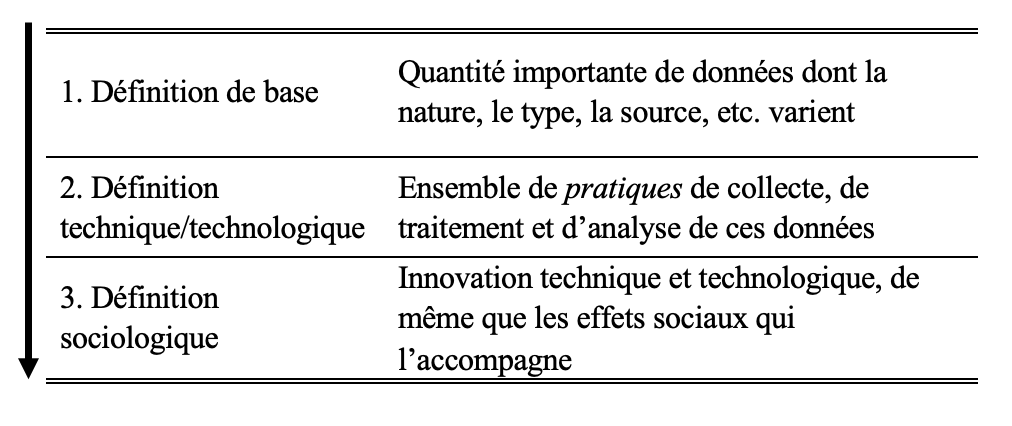
\includegraphics{images/chapitre1_definitions.png} 1. Premièrement, les
données massives représentent une \textbf{\emph{quantité importante de
points d'information}} qui varient selon la nature, le type, la source,
etc. Ici, la distinction entre données massives et données plus
traditionnelles (ou « non-massives ») est simplement quantitative.

\begin{enumerate}
\def\labelenumi{\arabic{enumi}.}
\setcounter{enumi}{1}
\item
  Deuxièmement, les données massives constituent un
  \textbf{\emph{ensemble de pratiques}} de collecte, de traitement et
  d'analyse de ces points d'information. Les données massives
  représentent une technique, c'est-à-dire une manière ou une méthode
  nouvelle de faire de la recherche.
\item
  Finalement, d'une perspective sociologique, les données massives
  représentent les impacts sociaux de ces importants développements
  technologiques. Cette perspective souligne le caractère
  essentiellement social des données massives, en portant notamment
  attention aux risques liés à la confidentialité des données, aux
  enjeux relatifs au consentement et à l'autorisation de collecte des
  informations, aux innovations en intelligence artificielle, etc.
\end{enumerate}

Dans les domaines scientifiques et technologiques, la définition
courante attribuée aux données massives intègre des éléments de ces
trois niveaux d'analyse en se référant à la composition et à la fonction
des données. Premièrement, la \emph{composition} des données massives
est généralement conceptualisée comme comprenant « 4V » : le volume, la
variété, la vélocité et la véracité. Cette conceptualisation jouit d'un
large consensus scientifique (Chen, Mao et Liu, 2014; Gandomi et Haider,
2015; Kitchin et McArdle 2016). Par ailleurs, plusieurs chercheurs ont
élargi cette définition de la composition des données massives en y
incluant, par exemple, la variabilité et la valeur des points de données
(Kitchen et McArdle 2016). Deuxièmement, la \emph{fonction} des données
massives comprend les innovations relatives à l'optimisation, à la prise
de décision et à l'approfondissement des connaissances qui résultent de
leur utilisation. Ces fonctions touchent des domaines sociaux
disparates, incluant le souci d'efficacité et de rendement des secteurs
privé et public ainsi que la recherche scientifique pure (Gartner 2012).

\section*{Les données massives et les sciences
sociales}\label{les-donnuxe9es-massives-et-les-sciences-sociales}
\addcontentsline{toc}{section}{Les données massives et les sciences
sociales}

\markright{Les données massives et les sciences sociales}

Dans le domaine des sciences sociales, les changements causés par
l'utilisation des données massives en recherche sont significatifs.
Plusieurs n'hésitent d'ailleurs pas à les qualifier de changements de
paradigme dans l'étude des phénomènes sociaux (Anderson 2008; Chandler
2015; Grimmer 2015; Kitchin 2014; Monroe et al.~2015). Dans le cas qui
nous intéresse, deux dimensions majeures méritent d'être abordées : (1)
une première relative à la validité (interne et externe) des données
massives et (2) une seconde relative à la différence entre les données
expérimentales et les données observationnelles. Ces deux dimensions
sont présentées de manière simultanées dans les prochaines sections.

\subsection*{La validité de la mesure en sciences
sociales}\label{la-validituxe9-de-la-mesure-en-sciences-sociales}
\addcontentsline{toc}{subsection}{La validité de la mesure en sciences
sociales}

La validité de la mesure constitue une exigence méthodologique centrale
à la recherche en sciences sociales. Les scientifiques cherchent
effectivement à s'assurer que ce qui est mesuré --- par un sondage, une
entrevue, un thermostat ou tout autre outil de mesure --- constitue bel
et bien ce qui est censé être mesuré. Adcock et Collier définissent plus
spécifiquement l'application de la validité de la mesure en sciences
sociales en affirmant que des scores (y compris les résultats de
classification qualitative) doivent capturer de manière significative
les idées contenues dans le concept correspondant (2001: 530).

Toutefois, les problèmes liés à la validité de la mesure sont nombreux
et ont une importance considérable. Dans l'étude des phénomènes sociaux
et humains, la validité de la mesure prend d'ailleurs une complexité
supplémentaire du fait que les données collectées par le biais d'une
mesure constituent le \emph{produit de l'observation} d'un phénomène,
mais non pas le phénomène en soi. Ainsi, lorsque, dans le contexte d'une
recherche, on propose de mesurer l'humeur de l'opinion publique (le
phénomène en soi) sur un enjeu politique, on utilise généralement un
sondage qui a pour fonction de mesurer le pouls d'un échantillon de la
population d'intérêt (ce qui est réellement observé). Cependant, ce que
ce sondage mesure ne constitue pas tout à fait l'opinion publique
elle-même, mais plutôt un segment populationnel qui se veut le plus
souvent représentatif de l'humeur de l'opinion publique. Ceci est tout
aussi vrai pour les sondages à petits échantillons que pour ceux
utilisant des données massives. Autrement dit, la mesure et les données
collectées ne représentent pas le phénomène --- l'opinion publique ---
en soi.

On a déjà mentionné que la validité de la mesure a de l'importance
puisqu'elle garantit que ce qui est mesuré représente réellement ce
qu'on croit mesurer. Toutefois, pour être plus spécifique, dans une
approche positiviste, la validité de la mesure se traduit généralement
par une logique de classification des valeurs attribuées aux différentes
manifestations distinctes d'un même phénomène. Par exemple, une mesure
de la démocratie comme celle proposée par \emph{Freedom House},
fréquemment utilisée en science politique, classifie les libertés
civiles et les droits politiques des États du monde par degré afin de
construire un index, ou une échelle, allant d'un autoritarisme complet à
une démocratie parfaite. Les scores représentent, dans ce contexte, une
mesure artificielle, mais ordonnée et logique, des idées contenues dans
le concept de démocratie telles que libertés civiles et droits
politiques. On peut ainsi dire que la question de la validité de la
mesure est un élément central de ce qui unit (1) le phénomène social
étudié (la démocratie), (2) son opérationnalisation (via les libertés
civiles et droits politiques) et (3) la méthode de mesure utilisée pour
observer et classifier d'une certaine façon le phénomène et les données
qui en découlent (dans le cas de \emph{Freedom House}, des codeurs
travaillant de manière indépendante les uns des autres).

\subsection*{La validité des données
massives}\label{la-validituxe9-des-donnuxe9es-massives}
\addcontentsline{toc}{subsection}{La validité des données massives}

En ce qui a trait aux données massives, la question de la validité de la
mesure constitue un défi nouveau. Les données massives ont en effet
comme avantage d'offrir aux chercheur.e.s soit de nouveaux phénomènes à
étudier, soit de nouvelles manifestations et nouvelles formes à des
phénomènes déjà étudiés. Les données massives permettent donc d'agrandir
la connaissance scientifique.

L'étude de King et al.~(2013) représente un cas éclairant de phénomène
social que l'utilisation des données massives permet désormais
d'étudier. En se basant sur la collecte de plus de 11 millions de
publications en ligne, King et ses collègues ont pu mesurer la censure
exercée par le gouvernement chinois sur ces réseaux sociaux. En
utilisant des données massives nouvelles, les auteurs ont donc pu
observer une manifestation inédite de censure massive qui, sans de
telles données, serait probablement demeurée mal comprise d'une
perspective scientifique. Le nombre de recherches basées sur
l'utilisation des données massives similairement innovantes en sciences
sociales est par ailleurs en croissance constante (Beauchamp 2017; Bond
et al.~2012; Poirier et al.~2020; Bibeau et al.~2021).

Cependant, il faut aussi souligner que les données massives, en raison
de leur complexité, peuvent avoir pour désavantage d'embrouiller l'étude
des phénomènes sociaux. Les opportunités scientifiques liées aux données
massives s'accompagnent en effet de certaines difficultés
méthodologiques. Parmi ces difficultés, trois enjeux sont
particulièrement cruciaux : (1) la validité interne, (2) la validité
externe et (3) la question d'un changement de posture ou d'orientation
épistémologique en sciences sociales causé par les données massives.

\subsubsection*{Validité interne des données
massives}\label{validituxe9-interne-des-donnuxe9es-massives}
\addcontentsline{toc}{subsubsection}{Validité interne des données
massives}

Premièrement, les données massives peuvent représenter un défi à la
validité interne des études en sciences sociales en rendant
pragmatiquement difficile l'établissement de \textbf{\emph{mécanismes
causaux clairs}}. Ce défi est notamment une conséquence du fait que la
plupart des données sont présentement issues d'un processus de
génération (\emph{data-generating process}) qui est hors du contrôle des
chercheur.e.s. Les données massives proviennent en effet habituellement
de sources diverses qui sont externes aux projets de recherche qui les
utilisent. Elles ne sont pas donc générées de manière aléatoire sous le
contrôle des chercheur.e.s.

Un des problèmes liés à cette situation est qu'il est difficile de
garantir une source \emph{exogène} de variation par laquelle les
chercheur.e.s éliminent l'effet potentiel des facteurs confondants
(\emph{confounders}). Règle générale, la distribution aléatoire d'un
traitement et d'un contrôle dans une expérience en laboratoire ou sur le
terrain représente le standard le plus élevé permettant de fournir cette
source exogène de variation, notamment parce qu'elle l'attribution
aléatoire du traitement ou du contrôle est entièrement sous le contrôle
du chercheur.e.s menant l'expérience. Cependant, en ce qui à trait à la
plupart des données massives, elles sont générées de manière
indépendante du contrôle du chercheur.e.s, et sont donc soumises aux
mêmes enjeux et problèmes (biais) que les données observationnelles
traditionnelles.

Pour le dire autrement, le défi de validité interne avec les données
massives constitue un enjeu relatif à la qualité des données. Ce n'est
évidemment pas un défi propre ou unique aux données massives. Ce défi
s'applique également aux autres types de données. Cependant, dans l'état
actuel des choses, le volume et la variété --- deux des 4V --- des
données massives --- textuelles, numériques, vidéos, etc. --- peuvent
miner la qualité de l'inférence causale entre une cause et une
conséquence que permet habituellement un processus contrôlé de
génération des données. En somme, la validité interne des données
massives est une fonction de la qualité de ces mêmes données.

\subsubsection*{Validité externe des données
massives}\label{validituxe9-externe-des-donnuxe9es-massives}
\addcontentsline{toc}{subsubsection}{Validité externe des données
massives}

Deuxièmement, les données massives représentent aussi un défi important
pour la validité externe des recherches en sciences sociales (Tufekci
2014; Lazer et Radford 2017; Nagler et Tucker 2015). Un des problèmes
les plus évidents concerne la \textbf{\emph{représentativité}} des
données massives collectées.

Comme le soulignent Lazer et Radford (2017), la quantité de données, en
soi, ne permet pas de corriger pour la non-représentativité des données.
Les données massives sont ainsi soumises au même problème de biais de
sélection que les autres types de données observationnelles, tels un
sondage ou une série d'entrevues, traditionnellement utilisés en
sciences sociales.

Le cas célèbre de l'erreur de prédiction du \emph{Literary Digest} lors
de la campagne présidentielle américaine de 1936 illustre bien ce
problème. Lors de cette campagne, le \emph{Literary Digest} a prédit à
tort la victoire du candidat républicain Alf Landon sur le président
démocrate sortant Franklin D. Roosevelt, puisque son échantillon de
répondants surreprésentait les électeurs plus aisés, traditionnellement
plus républicains, au détriment des électeurs moins aisés, plus
généralement proches du Parti démocrate. Cette erreur de
surreprésentation dans l'échantillon est due au fait que le
\emph{Literary Digest} a effectué un échantillonnage basé sur les listes
téléphoniques et le registre des propriétaires de voitures, biaisant par
le fait même l'échantillon au détriment des électeurs plus pauvres ne
possédant pas de téléphone ou d'automobile, mais qui constituaient un
électorat favorable à Roosevelt (Squire 1981). Le biais de sélection du
sondage a ainsi sous-estimé le soutien populaire de Roosevelt de plus de
20 points de pourcentage.

Aujourd'hui, l'utilisation des données massives est soumise aux mêmes
enjeux méthodologiques. L'accumulation massive de données ne permet pas
de compenser pour la qualité des données. Les données massives, comme
les données plus traditionnelles, sont soumises aux conséquences
induites par le processus de génération des données (\emph{data
generating process}) comme un échantillonnage.

Toutefois, depuis quelques années, le développement de nouvelles
méthodes de pondération des données offre des pistes de solutions. La
grande quantité de données massives permet notamment d'appliquer des
méthodes de pondération bien plus efficaces pour corriger les
échantillons non-représentatifs (Wang et al.~2015).

\subsection*{Données expérimentales}\label{donnuxe9es-expuxe9rimentales}
\addcontentsline{toc}{subsection}{Données expérimentales}

La question du processus de génération des données devient plus claire
quand on considère comment les \emph{données observationnelles} et les
\emph{données expérimentales} permettent d'effectuer des inférences de
manière distincte (voir Figure 2). Toutefois, pour bien comprendre ce
point, il faut comprendre les notions de données expérimentales et
d'inférence causale, qui sont centrales au domaine de la causalité en
recherche.

En quelques mots, l'essence de la démarche causale se résume comme suit
: le processus de génération de données expérimentales a pour objectif
d'assurer la validité d'une inférence causale estimée sur un échantillon
sur l'ensemble de la population visée.

Plus spécifiquement, le processus de génération des données permet aux
chercheur.e.s de s'assurer que la distribution du traitement entre les
deux groupes, traitement et contrôle, est entièrement aléatoire. De
manière technique, cette distribution aléatoire du traitement entre les
deux groupes permet de garantir une source exogène (à l'opposé de
endogène) de variation sur la variable indépendant (\emph{x). Cette
source exogène de variation permet, quant à elle, d'éliminer
l'endogénéité entre la variable indépendante (}x\emph{) et le résidu
(}e*).

Autrement dit, le fait de distribuer au hasard le traitement entre les
membres du groupe traitement et ceux du groupe contrôle assure que la
variation dans les résultats ne vient pas d'autres facteurs
non-contrôlés (le résidu, \emph{e}), mais plutôt du traitement lui-même
(la variable indépendante, \emph{x}). En distribuant le traitement de
manière aléatoire, on s'assure que les différences dans les résultats
sont vraiment dues au traitement et non à d'autres facteurs.

Il s'agit là d'assurer le respect de la condition d'indépendance,
essentielle à la validité de l'identification de l'effet causal étudié.
Autrement dit, en éliminant l'endogénéité entre la \emph{x} et \emph{e},
on s'assure que l'effet observé n'est pas dû à une variable confondante.

Pour revenir aux données massives, celles-ci ne peuvent pas résoudre les
enjeux liés aux inférences causales ou explicatives (Grimmer, 2015).
Elles sont en effet également soumises aux mêmes impératifs issus du
processus de génération des données.

\subsection*{Données
observationnelles}\label{donnuxe9es-observationnelles}
\addcontentsline{toc}{subsection}{Données observationnelles}

En ce qui a trait aux données observationnelles, il y a deux points
importants. Premièrement, des méthodes d'inférence basées sur des
approches par design (\emph{design-based methods}) comme une méthode de
régression sur discontinuité ou de variable instrumentale peuvent
également garantir des inférences explicatives et causales valides.
Elles nécessitent toutefois plusieurs postulats plus restrictifs dont
l'objectif est d'imiter ou de récréer, de la manière la plus fidèle
possible, une distribution aléatoire du traitement -- ce que la
littérature appelle un \emph{as-if random assignment} (comme si
l'attribution était aléatoire) (Dunning, 2008).

Dans un contexte observationnel, les données massives peuvent donc
permettre d'augmenter la précision des estimations causales.
Effectivement, comme dans un modèle de régression linéaire, plus
l'échantillon est grand, plus l'estimation du coefficient causal ou
probabiliste est précise. Par exemple, un échantillon large dans un
modèle de régression sur discontinuité permet de restreindre la largeur
de bande autour du seuil, garantissant ainsi une distribution presque
parfaitement aléatoire des données et une validité plus élevée à
l'estimation de l'effet causal.

Un autre exemple pourrait être l'utilisation du « matching », souvent
utilisé dans les études économétriques. Supposons que vous souhaitez
estimer l'effet d'un programme éducatif sur les résultats scolaires
d'étudiant.e.s. Le devis de recherche idéal serait d'assigner
aléatoirement les étudiant.e.s au programme (le groupe traitement) ou
non (le groupe contrôle). Toutefois, puisque ce devis idéal peut être
difficilement réalisable, un grand nombre de données pourrait permettre
de trouver pour chaque étudiant.e dans le groupe traitement un
étudiant.e « jumeau » dans le groupe contrôle. Ce « jumeau » serait
similaire en âge, sexe, antécédents socio-économiques, etc. Il serait
ensuite possible de comparer les résultats scolaires de ces jumeaux pour
estimer l'effet du programme. Plus l'échantillon est grand, plus
l'estimation sera précise et fiable, parce qu'il y aura plus de jumeaux
possibles à apparier, réduisant ainsi le biais dû aux variables non
observées.

Il s'agit d'un exemple où les données massives augmentent la validité
interne de l'étude, même si les données sont de nature observationnelle
et non expérimentale.

Deuxièmement, un échantillon de données massives observationnelles
issues d'une plateforme comme X --- anciennement Twitter --- ou Facebook
peut fournir une \emph{description} plus fine de certaines dynamiques
sociales observées sur les réseaux sociaux. Cependant, c'est la manière
dont sont collectées les données de cet échantillon de données massives
qui garantit la représentativité de l'échantillon --- avec pour objectif
l'absence d'un biais de sélection --- et non pas la quantité de données.
Généralement, le biais d'un échantillon est une conséquence de la
non-représentativité des répondants; dans notre exemple, les
utilisateurs des médias sociaux ne sont généralement pas représentatifs
de la population entière.

Dans un tel cas, des méthodes de pondération sur des données
observationnelles peuvent compenser pour la sur- ou la
sous-représentativité de sous-groupes dans un échantillon afin d'assurer
la validité de l'inférence entre échantillon et population. Les données
massives ont ici une importance puisqu'une pondération fiable nécessite
une quantité substantielle d'observations. Une pondération \emph{a
posteriori} sera donc plus fiable plus l'échantillon est grand. Les
données massives ont ainsi une valeur ajoutée afin d'établir des
inférences descriptives plus précises et sophistiquées.

\subsection*{Validité écologique et observation par
sous-groupes}\label{validituxe9-uxe9cologique-et-observation-par-sous-groupes}
\addcontentsline{toc}{subsection}{Validité écologique et observation par
sous-groupes}

Les données massives peuvent aussi jouer d'autres rôles importants
relatifs à la validité externe. Premièrement, les données massives
facilitent effectivement la validité externe de certaines études en
accroissant la validité écologique (\emph{ecological validity}) des
tests expérimentaux, c'est-à-dire le réalisme de la situation
expérimentale (Grimmer, 2015: 81). En effet, la variété des sources et
des formats de données permet aux chercheurs d'imiter plus fidèlement la
réalité sur le terrain vécue par les participants aux études.

Deuxièmement, la quantité importante de données rend possible
l'observation d'effets précis, spécifiques et inédits par sous-groupes
(Grimmer 2015: 81). Alors qu'auparavant, la taille réduite des
échantillons ne permettait pas d'effectuer des inférences valides pour
des sous-groupes de la population --- les écarts-types par sous-groupes
étaient trop grands, rendant difficile l'estimation précise d'un
paramètre comme la moyenne et impossible celle d'un coefficient ---, la
taille énorme des échantillons de données massives permet aux chercheurs
d'estimer des paramètres qui étaient demeurés extrêmement imprécis
jusqu'à aujourd'hui. Notre compréhension des phénomènes sociaux s'en
trouve par le fait même approfondie de façon considérable.

\begin{figure}[H]

{\centering 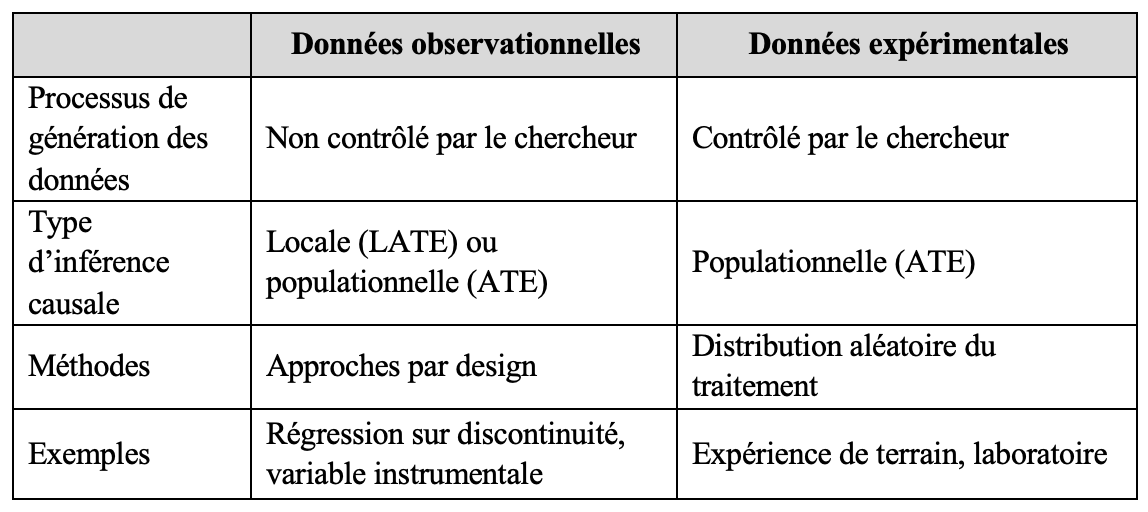
\includegraphics{images/chapitre1_tableau.png}

}

\caption{image2\_2}

\end{figure}%

\section*{Conclusion : trois questions ouvertes pour le
futur}\label{conclusion-trois-questions-ouvertes-pour-le-futur}
\addcontentsline{toc}{section}{Conclusion : trois questions ouvertes
pour le futur}

\markright{Conclusion : trois questions ouvertes pour le futur}

Comme nous venons de le voir, la quantité et la variété nouvelle des
données massives permettent à la fois un approfondissement de l'analyse
de certains phénomènes et l'ouverture de nouvelles avenues de recherche.
L'analyse des données massives peut permettre de mettre en lumière des
tendances subtiles échappant aux ensembles d'informations plus
restreints.

Il faut toutefois souligner que les données massives représentent une
complexification de l'analyse des phénomènes en sciences sociales d'une
perspective non pas seulement méthodologique/technique mais également
épistémologique.

Cela soulève au moins trois questions d'importance, dont les réponses ne
nous sont pas encore accessibles, pour l'avenir de la recherche en
sciences sociales : (1) les données massives entrent-elles
(partiellement du moins) en conflit avec l'impératif de parcimonie qui
caractérise la science moderne?; (2) ces données sont-elles dans la
continuité ou représentent-elles une coupure dans la tradition
béhavioraliste en sciences sociales (et en science politique tout
particulièrement)?; (3) et finalement, de manière reliée, les données
massives proposent-elles ou non une manière de dépasser l'individualisme
méthodologique qui caractérise les sciences sociales contemporaines?

\bookmarksetup{startatroot}

\chapter{Le logiciel libre et le code source ouvert}\label{sec-chap1}

Ce chapitre ne présentera pas un outil en soi. Il vise à initier les
lecteurs et les lectrices à la philosophie du logiciel libre et surtout
de situer ces réflexions dans le contexte de la recherche en sciences
sociales. En fait, l'outil ici est plutôt de l'ordre réflexif que
concret. À la fin de ce chapitre, les lecteurs et lectrices seront en
meilleures positions afin de situer les outils qui seront présentés dans
le grand univers des locigiels libres et payants. Ils et elles pourront
comprendre les motivations derrière le développement et l'utilisation de
tels logiciels. Sans vouloir divulgâcher quoi que ce soit, la création
et l'utilisation de logiciels libres dépassent le simple calcul coûts et
bénéfices utilitaires, gratuit contre payant. Tout cela s'inscrit dans
des réflexions philosophiques, éthiques et épistémologiques plus grandes
qui continuent, à ce jour, d'influencer les développeurs et les
utilisateurs. Nous verrons tout au long de ce chapitre que certaines de
ces motivations rejoignent la méthode scientifique, qui est au coeur de
notre quête de savoir et de compréhension du monde sociale (King et al.,
2021). Ainsi, ce chapitre jette la base réflexive qui est derrière les
choix des outils numériques présentés dans ce livre, où nous avons tenté
de joindre les avantages des logiciels libres avec certains qui sont
payants dans le but de créer un environnement de travail à la fois
individuel et collaboratif. Avant d'aller plus en profondeur, une
certaine distinction mérite d'être faite, qui permettra d'éviter
certaines confusions quant au but de ce livre et à la terminologie
utilisée.

Il est donc important de faire une première distinction entre une
méthode, dite méthodologique, et un outil numérique. La méthodologie est
le champ de la philosophie des sciences qui s'intéresse à l'étude des
méthodes scientifiques ou techniques. Celles-ci visent à collecter et à
analyser des données, suivant les impératifs scientifiques, et qui ont
pour but de contribuer au savoir et à la connaissance. Il faut faire
attention puisque parfois, dans certains livres ou dans certains
articles, il est possible que les auteurs ou les autrices parlent des
méthodes qu'ils et elles ont utilisées comme étant des \emph{outils}.
D'un point de vue méthodologique, lié à la philosophie des sciences, il
est approprié d'utiliser ce genre de vocabulaire. Ainsi, la régression
linéaire, le \emph{clustering}, les entretiens semi-dirigés et l'analyse
de contenu sont des méthodes. En revanche, les outils dits numériques
qui sont présentés dans ce livre ne sont pas des méthodes scientifiques.
Des outils numériques comme \texttt{R}, Dropbox ou GitHub ne sont pas
des méthodes. Ils sont des outils qui permettent de structurer sa
pensée, d'organiser son espace et son environnement de travail, et
d'implémenter son protocole de recherche afin de collecter et d'analyser
des données et d'en dériver des conclusions. Il n'est donc pas approprié
de considérer qu'un outil numérique est synonyme de méthode.

Ce livre, et par extension ce chapitre, ne vise pas à présenter des
\emph{outils méthodologiques} - compris ici comme étant des outils qui
permettent de \emph{désigner}, d'exécuter et d'évaluer une recherche
(Brady \& Collier, 2010). Ils visent plutôt à présenter des \emph{outils
numériques} qui, comme mentionnés dans le paragraphe précédent,
permettent de \emph{structurer sa pensée, d'organiser son espace de
travail et d'implémenter certaines méthodes}. Cette distinction est
importante pour le reste de ce livre, et surtout pour la compréhension
de son contenu. Les lecteurs et les lectrices, au fil des pages,
acquerront des compétences et du savoir à propos des outils numériques.
Celles-ci leur permettront de développer un nouveau langage à partir
duquel ils et elles pourront réfléchir et penser leur recherche, et
surtout interagir avec les autres personnes dans leurs champs; avec qui
ils et elles pourront plus aisément collaborer en organisant leur
environnement de travail; avec qui ils et elles pourront partager des
documents et leurs résultats.

Pour atteindre ces objectifs, il est important de commencer pas la base
- comprendre d'où vient le logiciel libre et qu'est-ce que c'est. Le
logiciel libre à une place importante dans les outils numériques, sans
parler de l'influence qu'il a eue et qu'il continue d'avoir aujourd'hui.
Afin de bien comprendre ce dont il est question, nous présenterons, dans
un premier temps, l'historique de cette philosophie et de ce mouvement
afin de le situer temporellement. De cette façon, nous pourrons mieux
comprendre ses motivations et ses revendications, mais aussi ses
influences actuelles. Ensuite, nous distinguerons le logiciel payant du
logiciel libre, pour ensuite aborder la différence entre le logiciel
libre et le code ouvert. Après coup, nous aborderons en quoi ces
réflexions sont intéressantes et importantes pour les sciences sociales
à l'ère du numérique, ainsi que les avantages et les inconvénients qui y
sont liés. À partir de cette section, nous pourrons montrer comment les
outils numériques s'inscrivent dans chacune des grandes étapes de la
recherche - avant, pendant et après. Finalement, avec ces quelques
notions en poche, nous présenterons les différents critères sur lesquels
nous nous sommes appuyés pour sélectionner les différents outils qui
sont présentés dans ce livre. Ces critères sont nés de la jonction entre
la philosophie du logiciel libre et l'expérience de recherche en tant
que chaire, dont avec la participation de collaborateurs externes.

\section{Logiciels Libres}\label{logiciels-libres}

\subsection{Le monde du libre}\label{le-monde-du-libre}

\emph{« Vous n'avez pas à suivre une recette avec précision. Vous pouvez
laisser de côté certains ingrédients. Ajouter quelques champignons parce
que vous en raffolez. Mettre moins de sel, car votre médecin vous le
conseille --- peu importe. De surcroît, logiciels et recettes sont
faciles à partager. En donnant une recette à un invité, un cuisinier n'y
perd que du temps et le coût du papier sur lequel il l'inscrit. Partager
un logiciel nécessite encore moins, habituellement quelques clics de
souris et un minimum d'électricité. Dans tous les cas, la personne qui
donne l'information y gagne deux choses : davantage d'amitié et la
possibilité de récupérer en retour d'autres recettes intéressantes. »} -
Richard Stallman (Williams et al., 2010)

Cette analogie illustre bien trois concepts au cœur de la philosophie de
Richard Stallman, souvent considéré comme le père fondateur du logiciel
libre : liberté, égalité, fraternité. Les utilisateurs de ces logiciels
sont libres, égaux, et doivent s'encourager mutuellement à contribuer à
la communauté. Ainsi, un logiciel libre est généralement le fruit d'une
collaboration entre développeurs qui peuvent provenir des quatre coins
du globe. Au centre de ce mouvement se trouve une réflexion éthique,
dont les militants font compagne depuis le début des années 1980, à
propos de la liberté des utilisateurs. La Free Software Foundation
(FSF), fondée par Richard Stallman en 1985, définit rapidement le
logiciel «libre» {[}free{]} comme étant garant de quatre libertés
fondamentales de l'utilisateur: la liberté d'utiliser le logiciel sans
restrictions, la liberté de le copier, la liberté de l'étudier, puis la
liberté de le modifier pour l'adapter à ses besoins et le
redistribuer\footnote{La redistribution doit évidemment respecter
  certaines conditions précises, dont l'enfreint peut mener à des
  condamnations
  {[}http://www.softwarefreedom.org/resources/2008/shareware.html{]}}.
Il s'agit ainsi d'un logiciel dont le code source\footnote{Pour rester
  dans les analogies culinaires, le code source est au logiciel ce que
  la recette est à un plat: elle indique les actions à effectuer, une
  par une, pour arriver à un résultat précis. Encore une fois, ce
  dernier peut-être adapté, modifié, bonifié.} est disponible, afin de
permettre aux internautes de l'utiliser tel quel ou de le modifier à
leur guise. L'accès au code source devient essentiel afin de permettre à
l'utilisateur de savoir ce que le programme fait réellement. Seulement
de cette façon, l'utilisateur peut \emph{contrôler} le logiciel, plutôt
que de se faire contrôler par ce dernier (Stallman, 1986).

\subsection{\texorpdfstring{Émergence et sémantique du
\emph{libre}}{Émergence et sémantique du libre}}\label{uxe9mergence-et-suxe9mantique-du-libre}

Plusieurs situent les débuts du mouvement du logiciel libre avec la
création de la licence publique générale GNU, en 1983, à partir de
laquelle va se développer une multitude de programmes libres. Parmi les
plus populaires, on retrouve notamment le navigateur Firefox, la suite
bureautique OpenOffice et l'emblématique système d'exploitation Linux,
qui se développe d'ailleurs à partir de la licence GNU\footnote{Pour une
  liste plus exhaustive, les lecteurs et lectrices peuvent aller
  consulter le répertoire du gouvernement du Canada:
  https://code.open.canada.ca/fr/logiciels-libres.html\#}. Aujourd'hui,
il s'agit d'un véritable phénomène sociétal: des milliers d'entreprises,
d'organisations à but non lucratif, d'institutions ou encore de
particuliers adoptent ces logiciels, dont la culture globale et les
valeurs (entraide, collaboration, partage) s'arriment avec le virage
technologique de plusieurs entreprises. Les logiciels libres ont
différents usages, en passant par la conception Web, la gestion de
contenu, les systèmes d'exploitation, la bureautique, entre autres. Ils
permettent donc de répondre à plusieurs types de besoins numériques et
informatiques.

Attention, le logiciel libre est avant tout une philosophie, voire un
mouvement de société. C'est une façon de concevoir la communauté du
logiciel, où le respect de la liberté de l'utilisateur est un impératif
éthique (Williams et al., 2010). Par conséquent, le terme libre,
\emph{free} en anglais, porte à confusion. Celui-ci ne signifie pas
qu'un logiciel libre est nécessairement gratuit. Certes, plusieurs sont
effectivement téléchargeables gratuitement. Toutefois, il est aussi
possible de (re)distribuer des logiciels libres payants. Par ailleurs,
aucun logiciel libre n'est réellement « gratuit » dans la mesure où son
déploiement et son utilisation nécessitent généralement différents
coûts, dont les degrés sont variables en fonction des compétences et de
l'infrastructure dont disposent les utilisateurs (coût d'apprentissage,
coûts d'entretien, etc.). Enfin, il est important de garder en tête que
les logiciels libres possèdent eux aussi une licence - cette dernière
est d'ailleurs garante des libertés que confèrent les logiciels libres
aux utilisateurs.

La grande liberté que ce type de logiciel offre favorise notamment la
collaboration entre les utilisateurs, et ce, à une échelle pouvant être
internationale. Les interactions entre les chercheurs créent une
dynamique d'« innovation ascendante » et d'entraide (Couture, 2014). En
d'autres termes, l'accessibilité et la collaboration favorisent le
développement et l'amélioration de ces logiciels. Selon certains, et
comparativement aux logiciels privés, les logiciels libres ont un niveau
plus élevé d'innovation (Smith, 2002). Contrairement aux logiciels
propriétaires, ceux qui se développent de manière privée et fermée, les
logiciels libres permettent à tous les utilisateurs de participer au
développement. Ceux-ci partagent ensuite leurs améliorations, ce qui
stimule à son tour de nouvelles initiatives. De plus, il est raisonnable
de penser que l'utilité des améliorations, ainsi que l'utilisation qui
en est faite par les utilisateurs, permet de générer un savoir
collaboratif (\textbf{couture20a?}).

Il y a aussi certains avantages économiques, dont un faible coût
d'acquisition et de renouvellement pour les particuliers. Cet avantage
individuel génère plusieurs externalités positives. Tout d'abord,
certains logiciels statistiques ainsi que certains programmes
informatiques coûtent plusieurs centaines, voire des milliers de
dollars, et dans certains cas doivent être renouvelés annuellement. Cela
augmente les coûts associés à l'utilisation du logiciel et par
conséquent limite son accessibilité. Comparativement, pour les logiciels
libres, la licence d'acquisition coûte bien souvent moins cher, et aucun
renouvellement de licence n'est demandé dans la plupart des cas.
L'argent sauvé des licences peut alors être investi dans le
développement du logiciel libre (Béraud, 2007). De plus, étant donné que
les chercheurs doivent souvent faire face à des contraintes budgétaires,
les logiciels libres deviennent des outils intéressants afin de
minimiser les coûts de la recherche (\textbf{yu\_munoz-justicia22a?}).
Il s'agit d'un avantage encore plus important et intéressant pour les
chercheurs dans les pays du Sud global (Santillán-Anguiano \&
González-Machado, 2023). L'accessibilité de ces ressources permet donc
de réduire l'écart dans la production scientifique entre les pays du Sud
et ceux du Nord. De plus, elle permet à tous de bénéficier d'outils
pédagogiques accessibles, ce qui favorise l'acquisition ainsi que le
développement de compétences méthodologiques.

Dans le cadre d'une formation universitaire, il peut être pertinent
d'enseigner aux étudiants à se servir de logiciel statistique ou
d'analyse de texte. L'acquisition de ces compétences peut être précieux
tant pour ceux et celles qui souhaitent se diriger vers le milieu
académique, que pour ceux et celles qui visent le marché professionnel.
D'ailleurs sur le site web de la banque d'emplois du gouvernement du
Canada, les conditions d'emplois sont en ce moment\footnote{En date
  d'écrire ces lignes, avril 2024.} très bonnes, et une pénurie de
main-d'œuvre est anticipée, entre 2022-2031, dans les emplois en analyse
de données. Ces compétences sont d'autant plus précieuses aujourd'hui,
dans le monde de données dans lequel nous vivons.

Il est important de souligner que la transition vers les logiciels
libres ne doit pas se faire seulement sur des bases économiques, mais
dans une perspective globale de changement de culture. Changer pour des
raisons purement économiques viendrait à violer l'essence même de la
philosophie du logiciel libre, qui se veut surtout être un esprit de
collaboration et de transparence. Par conséquent, il est important
d'incorporer aussi les valeurs et la philosophie dans notre utilisation.
Amélioration constante, entraide, savoir partagé et plusieurs milliers
de contributeurs (Couture, 2014), ces éléments résument très bien la
philosophie du logiciel libre.

\subsection{Illustrations}\label{illustrations}

Considérons quelques exemples de logiciels libres et de logiciels
payants afin de mettre en relief les trois éléments présentés ci-haut:
1) la liberté de l'utilisation et de la contribution, 2) les coûts
d'acquisition et 3) les compétences acquises et développées. Dans les
chapitres suivants, des outils numériques tels que \texttt{R}, SPSS,
STATA, qui permettent de mener des analyses statistiques, ou encore la
suite Office, Quarto, LaTeX, qui permettent de formater un document
écrit, seront présentés. Cette section ne remplace en aucun cas une
lecture approfondie et détaillée des chapitres suivants. Au besoin, nous
recommandons fortement aux lecteurs et aux lectrices de se référer au
reste du livre. En ce qui concerne le premier trio, \texttt{R} est le
seul logiciel libre du groupe. Il est accessible gratuitement à partir
du site web de CRAN, et une grande communauté d'utilisateurs contribue
activement à son développement. Par exemple, la compagnie Posit est
derrière le développement de \texttt{RStudio}, Quarto et
Positron\footnote{Un nouvel IDE, qui est toujours en cours de
  développement, qui souhaite offrir une interface optimisée pour
  \texttt{R} et Python construit sur VS Code} qui sont toutes des
extensions à code ouvert de \texttt{R}. Ensuite, plusieurs utilisateurs
ont développé des librairies avec des commandes et des fonctions
supplémentaires, qui sont gratuites et dont le code est disponible sur
des plateformes comme GitHub.

Contrairement à \texttt{R}, des logiciels comme SPSS et STATA, qui sont
des logiciels propriétaires, nécessitent une licence privée afin de
pouvoir les utiliser. L'achat d'une licence doit aussi être situé avec
ses propres besoins puisque, dans le cas de SPSS, les licences ne
donnent pas toutes accès aux mêmes fonctionnalités. Ainsi, la licence de
base ne donne pas accès à l'utilisation de la régression, alors que la
licence Premium le permet. De plus, la licence doit être renouvelée tous
les ans, et les prix varient entre 1 700\$ et 5 194\$ pour la licence
web à un seul utilisateur. En ce qui concerne STATA, la logique est
similaire à celle de SPSS. Différents types de licence sont offerts avec
des fonctionnalités supplémentaires, notamment en termes de rapidité de
l'exécution des fonctions et de la capacité à traiter une large quantité
d'observations. Les licences annuelles éducationnelles, donc pour les
étudiants, se situent entre 126\$ et 506\$ par année. Autrement, le prix
varie en 1 248\$ et 1 950\$ par année. De plus, SPSS et STATA sont
développés uniquement par les compagnies IBM et par StataCorp
respectivement. Bien qu'ils n'offrent pas la même flexibilité que
\texttt{R} et que les utilisateurs ne peuvent pas contribuer au
développement au même titre que \texttt{R}, ils offrent d'importantes
ressources pour les utilisateurs, notamment par l'entremise d'un service
à la clientèle, de documentations et de formation web, par exemple.
Ainsi, les utilisateurs sont ``pris en charge'' directement par la
compagnie afin de leur fournir de l'aide et du support.

En ce qui concerne les langages de balisage, LaTeX ou Quarto peuvent
être utilisés gratuitement sur des interfaces comme \texttt{RStudio} ou
VS Code. Ils offrent donc une grande flexibilité étant compatible avec
plusieurs interfaces. Ainsi, une fois que les compétences avec le
langage ont été développées, il est facile de les transposer d'une
interface à une autre. À l'inverse, la suite Office offre ses propres
interfaces qui sont plutôt intuitives, mais qui contraignent
l'utilisateur à des fonctions prédéfinies. De plus, le coût
d'acquisition d'une licence de la suite Office varie entre 79\$ et 109\$
par année. Similairement à STATA et SPSS, Microsoft offre plusieurs
ressources directement sur leur site web pour les utilisateurs. Ainsi,
un certain ``encadrement'' est offert par la compagnie.

Deux derniers éléments sont importants d'être soulevés. Il ne faut pas
penser que les logiciels libres sont dénués de support et de
documentations. La plupart des logiciels libres, et des extensions comme
les librairies sur \texttt{R}, offrent beaucoup de documentations, et
plusieurs forums d'utilisateurs partagent leurs problèmes et leurs
solutions. De plus, certains tutoriels sont disponibles sur YouTube ou
sur des plateformes comme Datacamp et CodeAcademy. Ainsi, les
utilisateurs ne sont pas totalement laissés à eux-mêmes. De plus,
plusieurs universités offrent des licences pour des logiciels, comme
Office ou SPSS, aux étudiants et aux étudiantes pour éviter que ceux-ci
aient à débourser d'importantes sommes supplémentaires afin d'acquérir
ces logiciels.

\subsection{Logiciel libre et code
ouvert}\label{logiciel-libre-et-code-ouvert}

Parallèlement au logiciel libre, il y a aussi le code ouvert, ou
\emph{open source}. A priori, la dénomination du logiciel libre et celle
du \emph{code ouvert} semblent suggérer qu'il s'agit de synonymes. Dans
les deux cas, le lecteur pourrait croire que l'on fait référence à des
logiciels, par exemple, qui sont exempts de restrictions d'utilisations
et auxquelles les utilisateurs peuvent participer au développement.
Cependant, il y a une distinction importante entre les deux.

Bien que les deux renvoient sensiblement aux mêmes types de logiciels,
les tenants de ces approches ne partagent pas la même perspective. Comme
Stallman (2022) l'explique, le logiciel libre est d'abord et avant tout
un mouvement qui fait « campagne pour la liberté des utilisateurs de
l'informatique ». Le code ouvert, quant à lui, met l'accent sur les
avantages pratiques, plutôt que de militer pour des principes.

Le terme \emph{code ouvert} sera introduit seulement en 1998 afin de
clarifier l'ambiguïté dans la dénomination « logiciel libre »
\footnote{Soit ceux qui ont été conçus suivant les principes
  philosophiques et « moraux » qui sous-tendent ce mouvement.},
\emph{free software} en anglais, afin de spécifier que le code source
était accessible, et non pas que le logiciel était « gratuit »
(\textbf{ballhausen19a?}). De plus, les logiciels à code ouvert doivent
respecter un certain nombre de critères quant à la distribution de leurs
logiciels (Open Source Initiative, 2006).

Rappelons tout d'abord que le logiciel libre se définit sur la base de
quatre libertés: 1) liberté d'utiliser le programme comme désiré; 2)
liberté d'étudier le fonctionnement du programme et de le modifier pour
ses propres besoins; 3) liberté de redistribuer des copies; 4) liberté
de distribuer des copies de la version « améliorer » du programme pour
ses pairs (\textbf{ballhausen19a?}). Concernant le \emph{code ouvert},
tout logiciel qui souhaite être inclus sous cette appellation doit
respecter dix critères: 1) Redistribution gratuite; 2) doit inclure le
code source; 3) doit permettre les modifications et les travaux dérivés;
4) l'intégrité du code source; 5) ne doit pas discriminer des personnes
et/ou groupes; 6) ne doit pas restreindre personne dans l'utilisation du
logiciel pour un domaine d'activité; 7) distribution d'une licence pour
l'utilisation; 8) la licence ne doit pas être spécifique pour un
produit; 9) la licence ne doit pas placer de restriction sur d'autres
programmes; 10) la licence doit être technologiquement neutre\footnote{Pour
  plus d'informations sur ces caractéristiques, nous encourageons les
  lecteurs à se référer au lien web de Open Source Initiative (2006).
  Ils y trouveront un contenu détaillé pour chacune des caractéristiques
  susmentionnées.} (Open Source Initiative, 2006).

Il est aussi utile de les distinguer des logiciels « non libres », soit
les logiciels propriétaires: « Son utilisation, sa redistribution ou sa
modification sont interdites, ou exigent une autorisation spécifique, ou
sont tellement restreintes qu'en pratique vous ne pouvez pas le faire
librement » (Système d'exploitation GNU, 2023). Par contraste, la
licence libre confère des droits de propriétaire. L'utilisateur a le
droit d'installer le logiciel sur autant d'ordinateurs que désiré, le
modifier selon ses besoins et le distribuer avec ou sans ses
modifications. Il peut même demander d'être payé pour distribuer des
copies, avec ou sans ses modifications.

Le logiciel libre et le \emph{code ouvert} ont certaines similitudes
puisqu'ils adhèrent tous les deux à la même vision du logiciel, ainsi
que de son accessibilité. Toutefois, il est important tout de même de
les distinguer puisqu'ils ont des origines différentes, et qu'ils mènent
à certaines pratiques qui sont différentes. La prochaine section utilise
un cas concret afin d'expliquer l'effet du libre, et l'utilité que cela
peut avoir.

\section{Les sciences sociales à l'ère du numérique: les enseignements
de la philosophie du logiciel
libre}\label{les-sciences-sociales-uxe0-luxe8re-du-numuxe9rique-les-enseignements-de-la-philosophie-du-logiciel-libre}

En quoi est-ce que ces deux concepts, issus du monde de l'informatique,
sont-ils intéressants et/ou important pour les sciences sociales ? Pour
répondre à cette question, il est important de retourner à la base, soit
de se questionner sur ce que constitue la recherche scientifique dans
les sciences sociales.

Dans leur célèbre ouvrage \emph{Designing Social Inquiry}, King et al.
(2021)\footnote{Ce livre est aussi connu sous l'acronyme \emph{KKV}, en
  référence à la première lettre du nom de famille de chacun des
  auteurs.} propose quatre critères qui définissent la recherche dite
scientifique: 1) le but est l'inférence; 2) les procédures sont
publiques; 3) les conclusions sont incertaines; 4) le contenu est la
méthode. La philosophie du code ouvert et les avantages pratiques du
logiciel libre s'arriment parfaitement avec plusieurs de ces critères.

Penchons-nous sur le critère de la transparence des procédures et celui
de la méthode comme étant le contenu. Plusieurs outils numériques
rendent possibles le partage et l'accès public des données et de la
méthode utilisée. Certains de ces outils seront d'ailleurs abordés dans
les chapitres suivants. L'accès aux données et aux procédures d'analyse
est un impératif scientifique. Comme nous l'aborderons un peu plus loin,
il y a toujours des concessions à faire lors des investigations
scientifiques. Par conséquent, un meilleur accès aux procédures et aux
données utilisées permet de cibler plus facilement les limites de
certaines recherches et de les combler lors de recherche ultérieure. De
plus, l'arrivée des données massives ouvre de nouvelles portes, mais
surtout de nouveaux défis relatifs à la validité interne et externe
ainsi qu'au type de données récoltées et à la validité écologique. Le
livre de Marres (2017) est très intéressant à ce sujet. Face au constat
que la vie sociale se trouve affecter par les changements numériques, il
nous faut en tant que chercheur du monde social réfléchir à notre façon
de comprendre les changements qui s'opèrent. Ainsi, face à ces défis,
une des solutions se trouve notamment dans un meilleur partage et dans
une meilleure accessibilité aux données et aux procédures.

Il est possible de faire certains liens avec les deux autres critères de
King et al. (2021). Premièrement, comme le but de la science est
l'inférence, soit tenter d'expliquer des phénomènes sociaux qui
s'inscrivent dans des catégories plus larges que nos observations
directes\footnote{Par exemple, les mouvements sociaux, le comportement
  électoral, les guerres et les révolutions, et bien plus.}, il est
important que nos conclusions soient soumises au plus grand nombre
possible et pas uniquement au comité éditorial d'une revue scientifique.
D'une part, la validité de nos résultats a un potentiel politique
important. Plusieurs décisions peuvent être prises sur la base des
connaissances et de la compréhension des dynamiques sociales. Il est
donc important que les résultats de recherche qui informent ces
décisions soient le plus rigoureux possible, et qu'ils aient été soumis
à l'examen critique par le plus grand nombre d'individus. D'autre part,
et comme King et al. (2021) le font remarquer, les conclusions sont
toujours incertaines. L'examen critique et la reproduction des
protocoles sont donc une nécessité dans ce contexte d'incertitude
constant. La science ne cherche pas à être dogmatique. Au contraire,
l'incertitude caractérise bien la science. Les résultats sont toujours
incertains, et ce que la recherche vise à faire c'est de renforcer notre
niveau de confiance envers certaines explications tout en écartant les
explications alternatives. Comme plusieurs de ces phénomènes ne sont pas
homogènes et qu'ils ne sont pas immuables, nous devons constamment
revoir les explications et notre compréhension de ces dynamiques.

Dans la même lancée, l'ouvrage \emph{Rethinking Social Inquiry} (Brady
\& Collier, 2010), une réponse à King et al. (2021), partage, en partie,
cette définition de la recherche scientifique. Pour les auteurs, les
scientifiques du monde social possèdent plusieurs outils qui leur
permettent de \emph{designer}, \emph{d'exécuter} et \emph{d'évaluer} une
recherche. Ces outils sont des procédures et des pratiques employées par
les chercheurs des traditions quantitatives et qualitatives. Ils ont
aussi des techniques analytiques qui leur permettent de \emph{développer
des preuves qui sont convaincantes}\footnote{L'objectif des auteurs est
  de permettre le dialogue et la réconciliation entre les tenants des
  deux principales traditions méthodologiques: les quantitativistes et
  les qualitativistes. D'où leur vision de la science comme se devant de
  développer des preuves qui seront considérées comme convaincantes par
  les chercheurs de ces deux traditions.}.

Chacun de ces outils a toutefois ses forces et ses faiblesses. Inspiré
de Przeworski \& Teune (1970), Brady \& Collier (2010) parlent ainsi de
\emph{compromis}. Selon eux, la pertinence d'un outil méthodologique
dépend de la question de recherche, du but de la recherche et de son
contexte. Le choix d'un outil, sur cette base, entraîne des compromis
qui empêchent d'atteindre tous les buts analytiques simultanément. Même
lorsqu'il y a adéquation entre la question et la méthode, plusieurs
autres embuches peuvent entraîner ces compromis, comme la disponibilité
des données par exemple, qui limitent par la suite la qualité et la
précision des résultats, ce qui explique, en partie, l'incertitude
envers les conclusions.

Il est intéressant de concevoir la réalité sociale comme étant un prisme
ayant un nombre infini de face. Chacune de ces faces correspond à une
compréhension partielle de la réalité. Pour y avoir accès, nous devons
utiliser une méthode de collecte et d'analyse de données, informées par
une question de recherche et/ou par la théorie\footnote{Nous préférons
  formuler la phrase ici en stipulant que le choix d'une méthode de
  recherche peut être informé par la théorie et notre question de
  recherche simultanément, mais peut aussi être fait seulement à partir
  d'une question de recherche. Cela fait référence à deux processus de
  recherche différents soit la méthode hypothético-inductive, et celle
  déductive.}. Étant donné que chaque outil méthodologique à ses limites
et que nous devons constamment faire des compromis, notre compréhension
de la réalité n'est que partielle une fois la recherche complétée. De
plus, il ne faut pas oublier que la compréhension que nous avons de
cette face reste incertaine.

En sommes, les enseignements de la philosophie du code ouvert, les
avantages pratiques du logiciel libre et les outils qui en découlent ont
le potentiel de permettre non seulement une plus grande transparence des
protocoles scientifiques, mais aussi un plus grand partage du savoir, et
ce, du début de la recherche jusqu'à la publication des résultats.

\section{Inconvénients et défis}\label{inconvuxe9nients-et-duxe9fis}

Jusqu'à présent, nous avons surtout présenté des avantages liés aux
logiciels libres. Toutefois, il n'y a pas que des points positifs, et ne
pas aborder certaines limites serait malhonnête.

\subsection{La courbe d'apprentissage}\label{la-courbe-dapprentissage}

Dans leur texte, Paura \& Arhipova (2012) soulèvent une critique faite
envers certains logiciels libres, notamment envers \texttt{R}. Le
problème principal d'enseigner les statistiques avec des logiciels
libres est qu'ils peuvent être compliqués à apprendre ainsi qu'à
utiliser; par conséquent, les étudiants passeraient plus de temps à
tenter de résoudre les erreurs de programmation plutôt que d'apprendre
les statistiques\footnote{Sur cet enjeu, nous conseillons aux lecteurs
  et lectrices de lire le chapitre 2 sur les langages de programmation
  ainsi que le chapitre 8 sur l'intelligence artificielle. Plusieurs
  trucs et astuces seront présentés dans ces chapitres.}. Il est vrai
que ces logiciels demandent un investissement en temps, afin d'être en
mesure de mener ses propres analyses statistiques. Par exemple,
\texttt{R} demande l'apprentissage d'un langage de programmation afin de
pouvoir utiliser le logiciel à son plein potentiel. De plus, la syntaxe
de certaines librairies demande aussi un certain temps d'adaptation. À
titre de comparaison, le logiciel SPSS offre une interface beaucoup plus
intuitive que \texttt{R}, dans lequel l'utilisateur peut simplement
cliquer sur les différents menus dans la barre d'outils afin de
sélectionner les analyses qu'il ou elle souhaite faire. SPSS présente
ses résultats dans des tableaux qui sont clairs et lisibles,
contrairement à \texttt{R} où plusieurs fonctions présentent les
résultats directement dans la console, sous un format moins
``esthétique''. De plus, la plupart des logiciels payants viennent avec
un certain service à la clientèle. En d'autres termes, lorsque les
utilisateurs rencontrent des problèmes techniques, ils peuvent se
référer au manuel d'utilisateur ou bien par l'entremise de l'assistance
technique qui est offerte par la compagnie. À l'opposé, la plupart des
logiciels libres ne sont pas accompagnés d'un service à la clientèle.
Les utilisateurs doivent donc se ``débrouiller'' par eux-mêmes
lorsqu'ils rencontrent des difficultés et des problèmes.

Toutefois, lorsque l'on compare le coût d'apprentissage avec les
bénéfices tirés, il est plus difficile de soutenir qu'il s'agit
uniquement d'un désavantage. Dans un premier temps, la syntaxe de
programmation de \texttt{R} n'est pas parmi les plus complexes à
apprendre, et elle s'intègre très bien avec certaines extensions, dont
Quarto ou RMarkdown, qui offrent de multiples possibilités pour
transmettre le résultat de ses recherches, que ce soit par l'entremise
d'un rapport, d'un article scientifique, un site web ou même un blogue.
Surtout, la logique derrière la syntaxe de base de \texttt{R} et celle
d'une nouvelle librairie reste sensiblement inchangée. Par conséquent,
lorsque nous avons une bonne compréhension du fonctionnement de base de
\texttt{R}, l'apprentissage d'une nouvelle librairie se fait
relativement rapidement. Certaine, comme \texttt{dplyr} du
\texttt{tidyverse} facilite grandement la manipulation des données
comparativement aux commandes de base. Dans un deuxième temps, en
comparant le coût, soit d'apprendre le langage de \texttt{R}, avec les
bénéfices, de mener ses propres analyses de données et de formater les
résultats pour les présenter, il est assez clair que tous ceux et celles
qui souhaitent, de près ou de loin, travailler avec des données
quantitatives, les bénéfices dépassent largement le coût. D'autant plus
que ces compétences s'inscrivent dans la longue durée, alors que
l'apprentissage est plutôt de courte à moyenne durée. Dans un troisième
temps, bien que certains logiciels offrent des alternatives plus
intuitives, elles n'offrent pas la même flexibilité que la plupart des
logiciels libres offrent. Pour résumer, bien que l'apprentissage d'un
langage de programmation demande un investissement en temps, les
bénéfices générés par ces nouvelles compétences dépassent le coût
initial. Finalement, bien que les logiciels libres n'offrent pas de
service à la clientèle, il existe bien souvent des forums d'utilisateurs
sur le web où il est possible de trouver des réponses à ses questions
et/ou de poser ses questions. Par conséquent, bien qu'il ne s'agit pas
d'un service directement offert par l'outil numérique en question, il
est toujours possible de trouver du support et de l'aide par l'entremise
de la communauté d'utilisateur.

\subsection{Problème de transparence}\label{probluxe8me-de-transparence}

L'arrivée des sciences informatiques a fait émerger des problèmes de
reproductibilité des protocoles scientifiques (Janssen, 2017). Le
problème principal est relatif à l'accès au code utilisé par les
chercheurs. Par exemple, il est possible de réaliser des analyses
statistiques avec \texttt{R} sans partager le code utilisé, ce qui
limite la transparence du processus scientifique. Dans cette situation,
il est difficile de savoir si des erreurs de codage ont été commises,
volontairement ou involontairement, affectant ainsi les résultats
partagés.

Afin de remédier à ce problème, certains outils tels que
GitHub\footnote{une plateforme publique \emph{code ouvert} sur laquelle
  nous pouvons héberger et partager notre code.} participent à la
transparence des résultats scientifiques
(\textbf{fortunato\_galassi21a?}). Ce logiciel permet aux chercheurs de
partager leur code afin qu'il puisse être accessible pour tous. Il est
important de mentionner ici que l'installation et la configuration de
GitHub peuvent s'avérer difficiles pour ceux et celles qui ne sont pas
initiés à l'informatique. Cela constitue une certaine barrière dans son
utilisation. Toutefois, nous souhaitons tout de même présenter l'utilité
de ce logiciel puisqu'il permet de rendre les processus ainsi que les
résultats de recherche plus transparents. Par exemple, si l'on réalise
une analyse statistique de la relation entre l'économie et le vote, nous
pourrions partager l'ensemble du code que nous avons utilisé sur GitHub.
D'une part cela permettrait aux utilisateurs de vérifier si les
résultats sont honnêtes, et d'autre part de réutiliser le code pour
mener leurs propres analyses.

Cependant, le partage du code reste encore majoritairement volontaire.
Janssen et al. (2020) soutiennent que plus d'effort et d'actions
concertés doivent être mis en place afin d'améliorer l'accessibilité aux
codes. Toujours selon ces auteurs, les journaux scientifiques pourraient
exiger que les auteurs rendent leur code public lors du processus de
publication. D'ailleurs, les résultats d'une expérience sur les facteurs
qui influencent les chercheurs à partager leur code démontrent que les
initiatives individuelles ne seront pas suffisantes pour une
augmentation du partage du code (\textbf{krahmer\_etal23a?}). Par
conséquent, rendre le code accessible devrait devenir un standard
institutionnalisé.

\subsection{Appropration capitaliste}\label{appropration-capitaliste}

Dans ce cas-ci, il s'agit plutôt d'un défi auquel le logiciel libre est
confronté plutôt qu'une critique quant aux limites de son utilisation.
En fait, l'accès au code source ainsi que la liberté et la possibilité
de contribuer au développement du logiciel constitue un avantage
intéressant pour les compagnies privées. Par conséquent, nous avons
assisté à une intégration partielle du logiciel libre dans la logique
capitaliste (Bessen, 2002; Broca, 2013). Certaines compagnies
profiteraient des utilisateurs comme une main-d'œuvre gratuite afin de
bonifier leur logiciel, ce qui permet, dans certains cas, de générer des
revenus commerciaux dont l'entreprise est la seule bénéficiaire
(\textbf{couture20a?}). Attention, il ne faut pas penser que toutes les
compagnies agissent de manière prédatrice. Le but ici est de souligner
que certaines pratiques commerciales trouble l'essence du mouvement du
logiciel libre, qui se veut davantage être un outil de collaboration
accessible, plutôt qu'un moyen pour générer des profits. Il est
important de garder en tête les valeurs et la philosophie qui a donné
lieu à ce mouvement.

\section{La chronologie de la
recherche}\label{la-chronologie-de-la-recherche}

Malgré ces limites et ces défis, nous pensons que les différents outils
numériques ont leur place en sciences sociales, et qu'ils s'inscrivent
parfaitement à chaque étape de la recherche. Bien que le partage soit
encore majoritairement sur une base volontaire, adopter cette pratique
dès maintenant est important pour s'engager vers une science plus
ouverte et transparente. Quant à cette dernière caractéristique, il ne
faut pas croire que le partage des résultats se limite à une conférence
ou à une publication scientifique. Bien au contraire, tout chercheur qui
souhaite être le plus transparent doit s'engager dans ce processus dès
la conception de sa recherche.

Avant de présenter différents outils qui existent pour cela, il faut
préciser en quoi la transparence et l'accessibilité sont bénéfiques pour
tous. D'une part, et comme nous l'avons présentée dans la section
précédente, la transparence est une caractéristique fondamentale de
toute recherche qui se veut scientifique. Elle est aussi liée à
l'intégrité du chercheur. Il est impératif de faire état du processus
qui mène à notre conclusion, de la sélection de nos données jusqu'à
l'analyse. C'est de cette façon que nous pouvons juger de la validité et
de la fiabilité des inférences, et surtout de ses limites. D'autre part,
la transparence favorise aussi l'apprentissage (King et al., 2021). De
rendre publique et accessible, à l'aide des outils numériques, les
données, le code et la ou les méthodes utilisées permet de contribuer
non seulement aux débats méthodologiques, mais aussi permet à d'autres
chercheurs d'apprendre sur l'utilité et l'utilisation de ces méthodes.

\subsection{Avant la recherche}\label{avant-la-recherche}

Au fil des prochains chapitres, les lecteurs et lectrices apprendront
une nouvelle langue. Au même titre qu'une langue comme le français,
l'anglais ou le japonais, ce langage permet de communiquer, et surtout
de réfléchir. De nouveaux concepts, une façon de penser et de réfléchir
à leur recherche, et surtout à son organisation. C'est au travers de la
langue que nous pouvons réfléchir. Ainsi, à l'aide de ces termes, les
lecteurs et les lectrices seront outillés pour concevoir leur recherche
et leur organisation avant même de l'entamer. De la visualiser dans
toute son ampleur, de cibler leurs besoins en fonction de leur but et de
leurs intérêts et ainsi organiser leur environnement de travail en
conséquence.

De plus, motivée par cet objectif inhérent à la science, la transparence
exige du chercheur un engagement dès les premières étapes de sa
recherche. Tout d'abord, il ou elle peut déjà établir son
\emph{workflow} en créant son dépôt GitHub dans lequel il rendra
accessibles son code et ses données. Plus d'informations seront
présentées dans le chapitre 3. Ensuite, une fois le \emph{design} de
recherche\footnote{Généralement, un design de recherche comprend les
  éléments suivants: Introduction, revue des écrits, problématiques, une
  question de recherche, un cadre théorique, des hypothèses ainsi qu'une
  section sur la méthode et les données utilisées.} fait, le ou la
chercheur peut le préenregistrer sur le site web de \emph{Open Science
Framework}\footnote{Lien vers le site web: https://osf.io}. L'objectif
de ce site web est que les chercheurs puissent faire état de leurs
hypothèses avant la collecte et l'analyse des données afin d'éviter
toute manipulation malhonnête \emph{post hoc}. Il s'agit d'un mécanisme
qui se veut contraignant afin que les chercheurs s'en tiennent à ce
qu'ils ou elles avaient prévu de mener comme recherche.

\subsection{Pendant la recherche}\label{pendant-la-recherche}

Une fois la recherche débutée, plusieurs outils s'offrent pour une
gestion efficace du flux de travail. Plusieurs d'entre eux seront
présentés dans les chapitres suivants. Ces outils permettent notamment
de sauvegarder les données et l'avancement du projet sur des serveurs
externes (le \emph{cloud}), comme Dropbox, afin d'éviter de tout perdre
en cas de problème. D'autres permettent de produire le matériel
nécessaire pour l'analyse de nos données, tel que R. Certains permet
aussi de partager avec des collaborateurs l'avancement de notre projet
et les scripts de nos analyses, comme Git et GitHub. D'autres permettent
de structurer notre texte pour la production d'un article scientifique
ou d'un chapitre de livre, comme Overleaf et Quarto. Ils permettent
notamment d'ajouter des tableaux et des graphiques tirés directement des
analyses, le tout dans un format respectant les exigences matérielles
pour la publication.

Nous ne voulons pas sous-entendre qu'il n'y a pas de limites à tous ces
outils. Chaque chapitre de ce livre présentera les points positifs et
négatifs des outils qui y seront abordés.

\subsection{Après la recherche}\label{apruxe8s-la-recherche}

Une fois l'article écrit et publié, les auteurs peuvent décider de
rendre accessible le matériel produit et utilisé en version gratuite sur
le web. Il s'agit du \emph{open science}, ou de la \emph{science
ouverte} (Chakravorty et al., 2022).

Cela permet de rendre non seulement les publications accessibles à tous
sur internet gratuitement, mais aussi les données utilisées, par
exemple, pour la réalisation de l'étude. Ces données peuvent ensuite
être réutilisées par d'autres chercheurs. Il s'agit d'avantages très
important, et surtout très prometteur. D'une part, un plus grand accès
au savoir scientifique aux décideurs publics permettra de prendre des
décisions qui s'appuient sur la science, et idéalement, sur une
pluralité de sources scientifiques afin de pouvoir évaluer adéquatement
les effets positifs et négatifs. Finalement, la réutilisation des
données peut réduire considérablement les coûts de la recherche. Bien
souvent, la production des données peut engendrer des coûts importants.
Par exemple, la production d'un sondage peut coûter plusieurs milliers
de dollars, et les données sont bien souvent utilisées qu'une seule fois
. Le partage des données de manière gratuite permet à des chercheurs qui
n'ont pas toujours les moyens de financer un sondage d'avoir accès à des
données. En somme, il s'agit de décloisonner le savoir des milieux
académiques. Ce qui vaut non seulement pour les publications, mais aussi
pour les données et les protocoles de recherche.

Toutefois, le libre accès reste confronté à certains défis. D'une part,
il y a un transfert de la charge financière qui se fait parfois vers les
chercheurs et les universités. Afin que les publications soient
accessibles en libre accès, les chercheurs et les universités doivent
souvent payer des sommes importantes. Cela soulève plusieurs questions
quant aux capacités des universités du Sud global et pour les chercheurs
hors universités, par exemple, de pouvoir assumer la charge financière
qui est liée à la publication en accès libre (Greussing et al., 2020;
Powell et al., s.~d.). D'autre part, bien que plusieurs pensent que les
données ouvertes et la science ouverte puissent contribuer à réduire les
inégalités dans la production du savoir entre le Nord et le Sud,
certains restent sceptiques quant à ce scénario. En fait, les données
ouvertes permettent de réduire les coûts d'accès aux données, mais ne
réduisent pas les coûts de production pour autant. Par conséquent, un
scénario évoqué par Serwadda et al. (2018) est un retour à la recherche
parachute\footnote{La recherche parachute est une « pratique extractive
  par laquelle des chercheurs - généralement issus de pays dotés de
  ressources élevées - effectuent des recherches et extraient des
  données et des échantillons de régions ou de populations non
  autochtones, généralement des contextes ou des pays à faibles
  ressources, sans reconnaître de manière appropriée l'importance de
  l'infrastructure et de l'expertise locales. Ce faisant, les chercheurs
  étrangers ne parviennent pas à établir des collaborations équitables
  et à long terme avec des partenaires locaux. »
  (\textbf{odenyTimeEndParachute2022?})}. En d'autres termes, les
chercheurs du Sud resteraient des acteurs de second plan, et qui pour
étudier leur propre société, devraient utiliser des données de
chercheurs du Nord qui auraient été produits sans la participation des
chercheurs locaux. Finalement, il y a aussi des enjeux quant à la
confidentialité des répondants et des utilisateurs Chiware \& Skelly
(2023). Plusieurs individus, comme dans le cas d'entretiens ou d'un
sondage, vont accepter de participer à l'enquête parce que leurs
réponses seront anonymisées et qu'elles ne seront pas partagées
publiquement. Tous ces éléments soulèvent d'importantes réflexions
éthiques quant aux bonnes pratiques à développer dans le cadre de la
science ouverte. La science ouverte à un avenir très prometteur et peut
générer des retombées positives, à conditions quelle s'intéresse aux
différents défis auxquels elle est confrontée.

\section{Critères de sélection}\label{crituxe8res-de-suxe9lection}

Au cours des prochains chapitres, plusieurs outils seront présentés.
Étant donné que le but de l'ouvrage n'est pas uniquement d'offrir une
perspective sur le monde du numérique, mais surtout d'offrir des
conseils pratiques aux lectrices et lecteurs, certains choix ont dû être
faits dans la sélection des outils. Bien que ces choix soient
arbitraires, ils sont tout de même informés par certains critères. Au
moment d'écrire ces lignes, peu de littérature existe sur le sujet. Par
conséquent, l'élaboration de ces critères s'est faite de manière
inductive, soit à partir de l'expérience des auteurs. Ils sont aussi
informés par des considérations pratiques, tels que la popularité de
l'utilisation par une communauté et par un champ d'études. Pour être
pleinement transparent, la grande majorité des autrices et auteurs de ce
livre sont issues de la science politique.

Malgré cela, nous pensons tout de même que ces critères sont pertinents
et informatifs pour les autres disciplines des sciences sociales. Par le
fait même, nous souhaitons introduire le débat avec les autres champs.
Nous sommes convaincus que ce dialogue sera riche et fructueux. Pour
l'instant, tenons-nous-en aux six critères ci-dessous. Tous les outils
présentés dans ce livre ne respectent pas nécessairement parfaitement
ces critères. Certaines considérations pratiques limitent le plein
respect de ces critères. Surtout, bien que le logiciel libre ait été mis
de l'avant tout au long de ce chapitre, ce ne sont pas tous les outils
numériques présentés dans ce livre qui sont des logiciels libres.
Certes, la philosophie du logiciel libre a influencé la sélection et
l'utilisation de ces outils, avant même la rédaction de ce livre.
Cependant, face à des contraintes pratiques, certains logiciels payants
sont utilisés et seront présentés. Bien évidemment, les logiciels libres
ne sont pas absolus. Ils peuvent cloisonner les chercheurs entre les
utilisateurs et les non-utilisateurs de ces logiciels. Un tel scénario
est loin d'être souhaitable. En aucun cas ils ne devraient limiter la
collaboration scientifique.

Les lectrices et lecteurs sont encouragés à réfléchir à propos de leur
propre besoin afin de déterminer quel.s outil.s elles et ils devraient
utiliser. Par exemple, si dans leur communauté, les gens utilisent
Python plutôt que R, alors nous recommandons d'utiliser Python. En
d'autres termes, les critères et les outils de ce livre ne visent pas un
dogmatisme, et un rejet total de tous les autres outils qui ne sont pas
couverts dans ce livre. Il est important d'évaluer ses besoins afin de
choisir quels outils devraient être utilisés.

\subsection{Accessibilité (Gratuit ou peu
dispendieux)}\label{accessibilituxe9-gratuit-ou-peu-dispendieux}

L'accessibilité au plus grand nombre de ces outils est importante pour
l'atteinte d'une science plus inclusive, et qui respecte les moyens de
chacun. L'accès à des outils de qualité ne devrait pas être caché des
verrous d'accès payants.

Cette accessibilité est aussi importante pour deux autres raisons. La
première, comme le livre vise à donner des connaissances pratiques dans
l'utilisation de ces outils numériques, il est important que les
lecteurs et lectrices aient facilement accès à ce qui sera présenté.
Cela permettra de reproduire au fur et à mesure de la lecture les
différentes étapes et pratiques qui sont présentées. La deuxième, est un
corolaire du premier, une fois ces compétences acquises, les lecteurs et
lectrices pourront facilement les réutiliser pour réaliser les diverses
tâches qu'ils et elles ont besoin d'accomplir.

\subsection{Existence d'une communauté
d'utilisateurs}\label{existence-dune-communautuxe9-dutilisateurs}

Ensuite, nous avons considéré l'existence d'une communauté d'utilisateur
pour les différents outils qui sont présentés dans ce livre. Ces
communautés permettent une grande collaboration entre les différents
utilisateurs, et servent souvent de forum d'aide lorsque des problèmes
surviennent. Par conséquent, les lecteurs et lectrices auront accès à
plusieurs forums d'aide sur internet, au besoin, pour la plupart des
outils qui sont présentés dans ce livre. Ainsi, au besoin, ils et elles
auront accès à des ressources supplémentaires en ligne lorsqu'une
question ou un problème surviendra.

Il se peut que certains logiciels libres n'aient pas un guide
d'utilisateur qui soit fourni avec le téléchargement du logiciel.
Parfois, cela peut être difficile pour ceux et celles qui souhaitent
apprendre à utiliser certains de ces outils de se retrouver et de
répondre aux questions qui surviennent. C'est pour ces raisons que nous
avons considéré l'existence d'une communauté d'utilisateurs, et
l'existence de forum d'aide sur le web. Par exemple, pour toutes les
questions liées au code, nous pouvons aller sur le site web de
\emph{Stack Overflow}, qui est un important forum d'échange, et sur
lequel nous pourrons trouver plusieurs informations et réponses à nos
questions.

\subsection{Popularité dans le champ}\label{popularituxe9-dans-le-champ}

Nous avons choisi certains outils sur d'autres notamment à cause de leur
popularité dans le champ et en sciences sociales. Par exemple, en
sciences sociales, pour les analyses quantitatives, c'est le logiciel R
qui est prédominant aujourd'hui. Non seulement dans son utilisation,
mais aussi dans les formations offertes, comme dans le cadre de l'école
d'été de la \emph{Inter-university Consortium for Political and Social
Research} (ICPSR). Par conséquent, il s'agit d'une considération
pratique. Dans le monde du numérique et de la programmation, certains de
ces outils deviennent une forme de langage. Ainsi, la maîtrise de ce
langage permet de dialoguer avec les autres chercheurs de notre champ,
ce qui favorise les débats et la recherche collaborative, par exemple.

\subsection{Compatibilité avec d'autres
outils}\label{compatibilituxe9-avec-dautres-outils}

Plusieurs des outils que nous présentons sont issus de notre expérience
de recherche. Nous utilisons plusieurs d'entre eux notamment parce
qu'ils permettent une certaine synergie dans le processus de la
recherche. Ainsi, ils s'intègrent bien les uns avec les autres et
permettent une connectivité. Par exemple, Zotero pour la gestion de sa
bibliographie et Quarto pour l'écriture de sa recherche se combinent et
permettent ainsi de sauver beaucoup de temps dans l'écriture et la
gestion des références. Cette intégration des différents outils est
importante puisqu'elle favorise non seulement la productivité et une
optimisation individuelle, mais aussi collaborative.

\subsection{Transparence et
réplicabilité}\label{transparence-et-ruxe9plicabilituxe9}

D'autres outils qui sont présentés visent à rendre accessibles les
résultats de recherche au plus grand nombre. C'est notamment le cas de
GitHub, qui sera présenté dans ce livre. Ces plateformes d'entreposage
permettent d'héberger des données et des bribes de code, ce qui favorise
la reproduction et la transparence des recherches. Ces éléments sont
importants pour la science en général, tout en s'inscrivant dans cet
objectif de science ouverte.

Cela favorise aussi l'apprentissage des gens qui souhaitent apprendre à
réaliser certaines analyses. Il est possible de trouver beaucoup
d'extrait de code sur ces plateformes, que nous pouvons tout simplement
copier-coller dans nos propres analyses. Ce faisant, nous pouvons
apprendre comment réaliser certaines tâches et performer certaines
analyses grâce à ces bribes. Il y a donc d'importantes externalités
positives qui sont produites en rendant accessible une partie de nos
efforts de recherche.

\subsection{Adaptabilité et
flexibilité}\label{adaptabilituxe9-et-flexibilituxe9}

Nous avons voulu présenter des outils qui ont la plus grande flexibilité
et adaptabilité possible. Nous souhaitons que tous et toutes puissent
trouver des outils qui puissent être adaptés à leurs besoins, immédiats
comme futurs. Cette adaptabilité est importante surtout lorsqu'on
considère l'investissement en temps qui est nécessaire pour la maîtrise
de ces outils. Il est donc important que cet apprentissage ne soit pas à
recommencer au complet chaque fois que nos besoins changent. Certes, il
se peut que certains approfondissements soient à faire dans le temps.
Cependant, ceux-ci devraient être minimes lorsque nous avons de bonnes
bases. La logique de plusieurs de ces outils reste inchangée, il s'agit
bien souvent d'apprendre une nouvelle commande, ce qui n'est pas très
coûteux en temps lorsqu'on connaît le :fonctionnement de l'outil. De
plus, plusieurs de ces outils permettent d'avoir un plus grand contrôle
sur la production et le formatage du texte et de graphiques, par
exemple. Cette flexibilité est un grand avantage lors de la rédaction et
de l'analyse des données.

\section{Conclusion}\label{conclusion}

En guise de conclusion nous souhaitons mettre l'accent sur un
apprentissage important qui se fait de manière implicite dans
l'acquisition de ces compétences pratiques: réfléchir de manière
scientifique. À la lecture de ce livre, les lecteurs et lectrices auront
fait des acquis très importants, et seront mieux outillés pour
réfléchir, organiser et produire leurs recherches, peu importe qu'elle
soit orientée vers le milieu académique ou professionnel. Nous pouvons
décliner le tout en trois principaux arguments.

Le premier concerne les gains à long terme. Nous avons déjà exposé, en
partie, cet argument dans la section des critères. Les outils que nous
présentons dans ce livre sont, pour la plupart, très versatiles. Nous
pouvons réaliser beaucoup de tâches avec ceux-ci. Bien qu'ils soient,
pour certains, coûteux en temps dans leur apprentissage, leurs bénéfices
dépassent largement leur coût. Le chapitre 7, à propos des langages de
balisage, approfondira ce point davantage, et expliquera pourquoi
l'apprentissage d'un langage comme \LaTeX~à ses bénéfices, en
comparaison avec Microsoft Word.

Le deuxième concerne la synergie entre tous ces outils. Comme nous
l'avons brièvement expliqué dans les critères de sélection,
l'apprentissage de ces différents outils favorise le développement d'une
synergie entre les différentes étapes et besoin d'une recherche;
notamment dans le développement de sa capacité à récolter, à entreposer,
à partager, à analyser et à publier ses données ainsi que ses résultats
de recherche.

Le troisième concerne le développement de sa « pensée de chercheur ».
Comprendre et maîtriser certains de ces outils permet de se doter de
capacités réflexives qui pourront être mobilisées dès les premiers
moments de la recherche, soit ceux de la conceptualisation. Dès qu'un
intérêt de recherche se développe nous pourrons déjà réfléchir à propos
de sa faisabilité, et de quelle manière pourrais-je récolter et analyser
des données qui me permettront de répondre à ma question. Cela permet
aussi de découvrir de nouvelles méthodes d'analyses de données.
Simplement par ces étapes préliminaires, nous gagnons beaucoup de temps
et d'itérations simplement par la capacité que nous avons à pouvoir
penser une recherche qui pourra être réalisée dans la mesure du
possible. De plus, ces acquis contribuent au développement de son
jugement critique et d'analyse, fort utile lorsqu'on lit des articles et
des ouvrages scientifiques. De cette façon, nous sommes en meilleure
position afin de mieux comprendre, d'analyser et de critiquer ce que les
autres chercheurs ont fait dans le cadre de leurs recherches.

\newpage{}

\bookmarksetup{startatroot}

\chapter{Langages de programmation}\label{langages-de-programmation}

\section{R ou ne pas R?}\label{sec-chap4}

Plusieurs notions liées à l'ère numérique, notamment à ce qui a trait
aux opportunités et difficultés que cette dernière peut amener, ont été
présentées par l'entremise du chapitre précédent. C'est un monde de
possibilité qui s'offre à ceux qui maîtrisent les nouveaux outils des
temps modernes. Mais comment en arriver là ? Le présent chapitre a pour
but de présenter certains outils flexibles et péreins permettant la
réalisation de nombreuses tâches. Une des premières étapes permettant de
notamment réaliser la collecte, l'analyse et la visualisation graphique
de données ainsi que la rédaction de documents est l'apprentissage d'un
langage de programmation. Bien que plusieurs langages de programmation
existent, le présent ouvrage priorise le langage \textbf{R}. Les
sections suivantes présentent ce langage de programmation, ces forces et
ces faiblesses ainsi que les raisons de son utilisation. Enfin, la
dernière section présente un environnement de programmation qui se prête
bien à son utilisation.

\section{Pourquoi R?}\label{pourquoi-r}

Comme mentionné précédemment, il existe plusieurs langages de
programmation. \textbf{R} a deux types de compétiteurs : les logiciels à
licences comme SAS, STATA et SPSS, et les langages \emph{OpenSource}
tels que Python et Julia. \textbf{R} est un langage de programmation
\emph{OpenSource} développé par des statisticiens, pour des
statisticiens, dans les années 1990 (Tippmann, 2015). \textbf{R} prend
ses racines dans le langage de programmation S, créé notamment par Ross
Ihaka et Robert Gentleman. Ces derniers ont fait des choix non
orthodoxes lors de l'élaboration du langage, qui font aujourd'hui la
popularité de ce logiciel auprès d'un large pan de la communauté
académique. En effet, Morandat et al. (2012) rapporte que le langage a
été élaboré afin qu'il soit intuitif et qu'il permette aux nouveaux
utilisateurs de rapidement réaliser des analyses.

Le langage de programmation \textbf{R} a plusieurs avantages qui font de
lui un outil puissant et utile pour tout chercheur. L'un de ses grands
avantages est qu'il est \emph{OpenSource}. Ayant déjà abordé le sujet
dans le chapitre précédent, il sera question ici de simplement rappeler
les grandes lignes de l'argument, à savoir que : 1) l'\emph{OpenSource}
est gratuit d'utilisation; 2) l'\emph{OpenSource} est développé de façon
bottom-up, ce qui lui procure une grande flexibilité; et 3) il permet
aux utilisateurs de créer leurs propres fonctions. À l'inverse, les
logiciels à licences sont coûteux, rigides et l'ajout de fonctionnalités
se fait par les développeurs internes à la compagnie. Ces formalités
rendent le processus plus lent et réduisent l'éventail des possibilités
pour la personne chercheuse. Ceci étant dit, certains avanceront que
c'est justement ce processus interne lent qui assure la validité et la
fiabilité des analyses effectuées par SAS, STATA ou SPSS. Or, dans son
livre dédié aux utilisateurs de SPSS et de SAS, Muenchen (2011) soulève
le point que bien souvent, ce sont des individus atomisés qui
développent les nouvelles fonctionnalités de ces langages et que le
processus de révisions se fait ensuite par des comités internes de
testeurs. Il en va de même pour le développement des \emph{packages} R
dans la mesure où ce dernier se voit testé et amendé par plusieurs
programmeurs indépendants dans un processus itératif des plateformes
telles que GitHub. De plus, bien des nouvelles techniques statistiques
sont développées pour R par des chercheurs qui publient leur travail
dans des journaux académiques revus par des pairs, assurant la qualité
du procédé. Le fait que SAS et SPSS permettent à leur utilisateur
d'intégrer des routines R à leur programme est un indicateur fort ne
serait-ce que de l'utilité de R (Muenchen, 2011). Le langage de
programmation \textbf{R} permet également de réaliser une grande
quantité de tâches de recherche. En effet, les personnes programmant en
\textbf{R} peuvent notamment manipuler et visualiser des données, faire
différents types d'analyses, créer des fonctions et faire des boucles en
plus de pouvoir combiner \textbf{R} avec certains langages de balisages.

D'un autre côté, l'utilisation du langage de programmation \textbf{R}
peut être perçue comme ayant certains inconvénients. Plusieurs disent
que la courbe d'apprentissage peut être plus grande que celle de
programmes à licences. La véridicité de cet argument est discutable. Les
programmes demandant des licences ont également un coût d'entrée. De
plus, les nouvelles itérations de ces logiciels amènent des changements
demandant une période d'adaptation pour la personne chercheuse. D'autres
disent que le développement \emph{OpenSource}, spécifiquement celui du
langage de programmation \textbf{R}, se fait de façon anarchique. Cela
est davantage une question d'opinion et de conception du monde qu'une
vérité. Le développement de \emph{package} se fait effectivement de
manière décentralisée et toute personne sachant programmer en \textbf{R}
peut collaborer à cette communauté. Bien qu'il n'y ait pas d'autorité
centrale, les \emph{packages} sont regroupés sur le \emph{Comprehensive
R Archive Network} (CRAN) (voir le https://cran.r-project.org/ pour plus
d'information). Le site a une politique de dépôt stricte, ainsi les
\emph{packages} doivent être suffisamment documentés. Il est également
possible d'y télécharger le langage de programmation \textbf{R}. Ce
langage, ainsi que ces différents \emph{packages}, sont disponible sur
Windows, macOS et Linux.

\section{Où coder en R ?}\label{ouxf9-coder-en-r}

Un environnement de développement intégré (IDE) permet aux programmeurs
de consolider les différents aspects de l'écriture d'un programme
informatique. Ils permettent de réaliser toutes les activités courantes
d'un programmeur -- l'édition du code, la construction des exécutables
et le débogage -- au même endroit. Les environnements de développement
intégrés sont conçus pour maximiser la productivité du programmeur. Ils
fournissent de nombreuses fonctionnalités -- notamment la coloration
syntaxique ainsi que le contrôle de version -- pour créer, modifier et
compiler du code. Certains environnements de développement intégré sont
dédiés à un langage de programmation spécifique. Par conséquent, ils
contiennent des fonctionnalités qui sont plus compatibles avec les
paradigmes de programmation du langage auquel ils sont associés. Enfin,
il existe de nombreux environnements de développement intégré
multilingues.

Comme mentionné précédemment, R est un des langages de statistiques et
d'exploration de données les plus populaires en sciences sociales. R est
pris en charge par de nombreux environnements de programmation.
Plusieurs ont été spécialement conçus pour la programmation en R -- le
plus notable étant RStudio -- tandis que d'autres sont des
environnements de programmation universels -- tels que Visual Studio
Code -- et prennent en charge R via des plugins. Il est également
possible de coder en R à partir d'une interface en ligne de commande.
Une telle méthode permet la communication entre l'utilisateur et son
ordinateur. Cette communication s'effectue en mode texte : l'utilisateur
tape une « ligne de commande » -- c'est-à-dire du texte dans le
\emph{terminal} -- pour demander à son ordinateur d'effectuer une
opération précise, telle que rouler un fichier de code R.

La suite du chapitre présente RStudio, notamment à travers ses avantages
et inconvénients, mais également des exemples de ses fonctionnalités.

\section{Qu'est-ce que RStudio ?}\label{quest-ce-que-rstudio}

RStudio est un projet open source destiné à combiner les différentes
composantes du langage de programmation R en un seul outil (Allaire,
2011). RStudio fonctionne sur tous les systèmes d'exploitation, y
compris Windows, Mac OS et Linux. En plus de l'application de bureau,
RStudio peut être déployé en tant que serveur pour permettre l'accès Web
aux sessions R s'exécutant sur des systèmes distants (Allaire, 2011).
RStudio facilite l'utilisation du langage de programmation R en offrant
de nombreux outils permettant à son utilisateur d'aisément réaliser ses
tâches. Parmi les plus utiles, on retrouve notamment une fenêtre d'aide,
de la documentation sur les différents packages R, un navigateur
d'espace de travail, une visionneuse de données et une prise en charge
de la coloration syntaxique (Horton, Kleinman, 2015). De plus, RStudio
permet de coder dans plusieurs langages et de supporter une grande
quantité de formats. Il fournit également un support pour plusieurs
projets ainsi qu'une interface pour utiliser des systèmes de contrôle,
tels que GitHub (Horton, Kleinman, 2015).

RStudio a plusieurs avantages. Son utilisation est facile à apprendre
pour les débutants. Les principaux éléments d'un IDE sont intégrés dans
une disposition à quatre volets (Verzani, 2011). Cette disposition
comprend une console, un éditeur de code source à onglets pour organiser
les fichiers d'un projet, un espace pour l'environnement de travail et
un quatrième volet où il est notamment possible d'afficher des
graphiques ou de la documentation sur différents packages. Ce volet
permet d'ailleurs d'accéder au répertoire des \emph{packages}
disponibles pour \emph{R} en plus de permettre à l'utilisateur de
consulter l'arborescence de ses fichiers. De plus, on y retrouve la
possibilité de créer plusieurs espaces de travail -- appelés projets --
qui facilitent l'organisation de différents \emph{workflows}.

Il y a plusieurs autres aspects de RStudio que les programmeurs
apprécient. Parmi ceux-ci se trouve le fait qu'il peut être utilisé via
un navigateur Web pour un accès à distance (Verzani, 2011). De plus,
RStudio supporte plusieurs langages de programmation ainsi que
différents langages de balisage. Qui plus est, de nouvelles
fonctionnalités sont régulièrement ajoutées pour satisfaire les besoins
de la communauté scientifique. Enfin, R logiciel est également souvent
mis à jour.

Parmi ce que certains considèrent comme étant les points faibles de
RStudio, on retrouve des éléments liés à la configuration. Certains
utilisateurs trouvent que le nombre de raccourcis est limité. D'autres
trouvent que le \emph{set up} des différents panneaux n'est pas
ergonomique, ou même qu'il n'est pas possible de pouvoir suffisamment
personnaliser l'environnement de programmation. De plus, certains
utilisateurs ont rapporté que RStudio était plus lent que d'autres
alternatives pour quelques opérations, surtout celles comprenant de
longs codes.

\section{Comment utiliser RStudio ?}\label{comment-utiliser-rstudio}

Bien que de nombreux éléments puissent être personnalisés, la
disposition par défaut de RStudio est composée de quatre volets
principaux (Verzani, 2011). Dans le coin supérieur gauche se trouve le
cadran principal. C'est dans celui-ci que l'utilisateur passera la plus
grande partie de son temps. On y modifie des fichiers de différents
formats et il est possible d'y afficher des bases de données. Dans le
coin inférieur gauche se trouve la console ainsi que le terminal. Dans
cette première, on peut interagir avec R de la même manière que dans le
cadran principal, mais le code ne sera pas enregistré. Le terminal, pour
sa part, est le point d'accès de communication entre un usager et son
ordinateur. Bien que les différents systèmes d'exploitation viennent
avec un terminal déjà intégré, il est aussi possible d'y accéder à
partir de RStudio.

On retrouve, dans le coin supérieur droit, l'espace de travail. Ce
cadran contient trois éléments : l'\emph{environnement global,
l'historique et les connections}. L'\emph{environnement global} est
l'endroit où l'utilisateur peut voir les bases de données, les fonctions
et les différents autres objets R qui sont actifs. Il peut cliquer sur
les divers éléments actifs pour les consulter. L'onglet
\emph{historique} permet à l'utilisateur de consulter les derniers
morceaux de code R qu'il a roulé ainsi que les dernières commandes
écrites dans la console. L'onglet \emph{connections}, pour sa part,
permet de connecter son IDE à une variété de sources de données et
d'explorer les objets et les données qui la composent. Il est conçu pour
fonctionner avec une variété d'autres outils pour travailler avec des
bases de données en R dans RStudio.

Le cadran dans le coin inférieur droit, pour sa part, contient plusieurs
outils très utiles pour les usagers de RStudio. L'onglet \emph{Files}
permet à l'utilisateur de naviguer dans les fichiers que contient son
ordinateur sans avoir à sortir de RStudio. L'onglet \emph{Plots} permet
de visualiser les graphiques générer à partir de R, que ce soit en
utilisant \emph{ggplot2, lattice ou base R}. L'onglet \emph{Packages}
permet de consulter les packages installés précédemment par
l'utilisateur en plus de pouvoir en consulter la documentation. C'est
aussi un des différents endroits à partir d'où il est possible
d'installer des packages avec RStudio. L'onglet \emph{Help} permet à
l'utilisateur de chercher et de consulter de la documentation sur de
nombreux sujets, notamment sur les différentes fonctions en R ainsi que
sur les packages. Pour sa part, l'onglet \emph{Viewer} permet la
visualisation de contenu web local.

Enfin, l'utilisateur peut modifier les dimensions par défaut pour chacun
des quatre cadrans principaux. En cliquant sur la division des sections,
il est possible d'ajuster l'allocation horizontale de l'espace. De plus,
chaque côté dispose d'un autre séparateur pour ajuster l'espace
vertical. Qui plus est, la barre de titre de chaque cadran comporte des
icônes pour ombrer un composant, maximiser un cadran verticalement ou
modifier la taille des l'espace de travail (Verzani, 2011; Nierhoff et
Hillebrand, 2015).

\section{Conclusion}\label{conclusion-1}

Le langage de programmation R est un outil très utile pour toutes sortes
de tâches notamment reliées aux statistiques et à la visualisation
graphiques. Sa maîtrise est requise pour accéder à plusieurs emplois,
autant dans le monde académique que dans les secteurs publics et privés.
Avec un peu de chance, le présent chapitre vous a éclairé sur son
utilité et sa pertinence dans le monde du travail contemporain. Bien que
le langage de programmation R ne doivent pas obligatoirement être
utilisé avec RStudio, nous pensons que pour la plupart des usagers, leur
utilisation conjointe est bénéfique et souhaitée. RStudio permet
également d'utiliser différents langages de balisage compatibles avec R,
facilitant l'utilisation de plusieurs outils complémentaires.
L'apprentissage du langage de programmation R apparaît également être
une valeur sure. Sa longitivité dans plusieurs sphères ainsi que la
forte croissance de sa base d'usagers laisse présager que d'en connaître
au moins les bases est un énorme avantage pour tout le monde. Pour ceux
qui sont particulièrement intéressés par le langage de programmation R
et qui désirent s'impliquer dans sa communauté, il existe plusieurs
conférences internationales et nationales sur R -- notamment
\emph{RConference} and \emph{useR!} -- et un journal académique,
\emph{The R Journal}. On retrouve également différentes communautés
telle que \emph{R-Ladies} qui met de l'avant la diversité des genres
dans la communauté du langage de programmation R. Le langage de
programmation R est plus qu'un simple outil statistique, il est le
centre d'une grande communauté de gens qui ont à coeur des principes
liés à l'inclusion et à l'avancement humain.

\bookmarksetup{startatroot}

\chapter{Outils de gestion de projet}\label{outils-de-gestion-de-projet}

\section{À la quête de l'optimisation}\label{sec-chap3}

Le monde de la recherche en sciences sociales numériques est en
constante évolution, offrant de nouvelles opportunités mais aussi des
défis uniques. Dans cette quête incessante pour optimiser notre
efficacité et notre collaboration, l'utilisation des bons outils devient
la clé de la réussite. Que vous soyez un chercheur en herbe ou un
professionnel chevronné, la manière dont vous organisez vos méthodes de
travail et gérez vos ressources peut déterminer la qualité et l'impact
de vos résultats.

\section{L'importance d'une méthode de travail
efficace}\label{limportance-dune-muxe9thode-de-travail-efficace}

Avant même de plonger dans les détails des méthodes de recherche et des
analyses, il est crucial de poser les bases d'une méthode de travail
efficace. Qu'il s'agisse de travailler en solitaire ou en équipe,
l'ordre et la structure sont des éléments essentiels. Des dossiers bien
organisés, une arborescence claire et un entreposage sécurisé deviennent
les piliers sur lesquels repose votre productivité. Après tout, un
environnement de travail organisé engendre des résultats ordonnés.

Ce chapitre vous emmènera à découvrir une gamme d'outils conçus pour
répondre aux besoins spécifiques des chercheurs en sciences sociales
numériques. Dans une quête pour maximiser votre temps, améliorer vos
flux de travail et renforcer vos collaborations, nous explorerons trois
types d'outils qui vous guideront dans cette quête d'optimisation~:

\begin{enumerate}
\def\labelenumi{\arabic{enumi}.}
\item
  \textbf{Logiciels de communication}~: La communication transparente
  est le cœur d'une collaboration réussie. Nous explorerons des outils
  tels que Slack qui facilitent les échanges en temps réel, connectant
  les chercheurs, même à distance, pour un partage rapide d'idées et
  d'informations.
\item
  \textbf{Logiciels de gestion de versions décentralisé}~: Nous
  plongerons dans le monde de Git et GitHub, des outils indispensables
  pour le suivi des versions et la collaboration efficace sur le code
  source.
\item
  \textbf{Outils d'entreposage de données}~: Que vous traitiez des
  données sensibles ou non, la conservation sécurisée de vos
  informations est primordiale. Des plateformes telles que Dropbox et
  Amazon Web Services (AWS) offrent des espaces sécurisés pour
  entreposer et partager vos données avec votre équipe.
\end{enumerate}

Chacun de ces outils est une pièce du puzzle, conçue pour vous aider à
gagner du temps, à collaborer de manière plus fluide et à renforcer la
qualité de votre recherche en sciences sociales numériques. Plongeons
dans ces outils avec un désir commun d'optimisation et d'excellence dans
notre travail.

\section{Gestion Individuelle}\label{gestion-individuelle}

\subsection{Gestion de tâches}\label{gestion-de-tuxe2ches}

Structurer ses tâches est un processus fondamental pour mener un projet
à terme. Particulièrement dans le monde académique, où les travaux
s'échelonnent souvent sur plusieurs années, il est facile de perdre de
vue ses objectifs ou de prendre des détours coûteux en temps si le
chemin vers le produit final est mal défini. Gérer et structurer ses
tâches de manière efficace facilite la mesure des progrès et permet de
constamment vérifier si ceux-ci sont encore alignés avec les objectifs
finaux.

\subsubsection{Comment}\label{comment}

Gérer ses tâches de façon efficace passe par une structuration claire
des objectifs du projet. Il est important de connaître la destination
finale afin de choisir la meilleure direction pour y parvenir. Pour ce
faire, il est utile de schématiser ou de lister la conception de la
version finale du projet. Dans l'idéal, à quoi ressemble-t-il dans sa
forme aboutie? Une fois cette vision clairement définie, il est possible
de désagréger le projet en grandes étapes. Que faut-il accomplir, à
l'échelle macro, pour atteindre les objectifs fixés?

À cette étape, il est crucial de prendre en compte les ressources
financières, temporelles et humaines disponibles. Cela permet de
déterminer de manière réaliste ce qui est possible. Identifier ces
grandes étapes contribue à la création d'un plan de projet structuré où
chaque phase est clairement définie. Cela aide à anticiper les besoins
en ressources et à ajuster les échéances en conséquence.

La révision continue est également un élément clé du processus de
gestion des tâches. En réévaluant régulièrement l'état d'avancement du
projet par rapport au plan initial, il est possible d'apporter des
ajustements nécessaires pour rester sur la bonne voie. Cet astuce permet
de répondre aux changements inévitables qui surviennent au cours de la
recherche, qu'ils soient dus à des découvertes inattendues, des
changements dans les directives institutionnelles ou des feedbacks des
pairs.

\subsubsection{Quand}\label{quand}

Avec des objectifs bien définis et des étapes claires pour y parvenir,
la structure du projet est complète. Il est donc temps de se lancer dans
la gestion des tâches. En fonction des objectifs établis, certaines
tâches sont plus importantes que d'autres. En effet, un projet est
vraissemblablement composé de tâches qui doivent être réalisées avant
que d'autres soient amorcées. Le défi est de déterminer efficacement ce
qui doit être priorisé. L'agilité est un processus de travail qui
facilite cette priorisation. En agilité, des objectifs sont fixés dans
le temps, et sont évalués de manière constante. Les tâches sont
déterminées en fonction de l'avancement et des blocants des objectifs.

Avec des objectifs bien définis et des étapes claires pour y parvenir,
la structure du projet est complète. Il est donc temps de se lancer dans
la gestion des tâches. En fonction des objectifs établis, certaines
tâches sont plus importantes que d'autres. Un projet est généralement
composé de tâches qui doivent être réalisées dans un ordre spécifique,
où certaines doivent impérativement précéder d'autres. Le défi est de
déterminer efficacement ce qui doit être priorisé pour maintenir une
progression fluide et efficace.

L'agilité est un processus de travail qui facilite cette priorisation.
En adoptant une approche agile, les objectifs sont fixés dans le temps
et sont constamment évalués. Cela permet une adaptation rapide et une
réponse aux changements sans compromettre les résultats finaux. De cette
façon, les tâches sont déterminées et ajustées en fonction de
l'avancement du projet et des éventuels obstacles rencontrés. Le projet
avance de façon incrémentale.

Pour une mise en œuvre efficace de l'agilité, il est utile de planifier
ses objectifs sur une période de quelques semaines, connues sous le nom
de sprints en méthode Scrum, où on évalue le travail accompli et on
redéfinit les priorités pour la prochaine période. Ces sprints
permettent de s'assurer de rester concentré sur les tâches qui apportent
le plus de valeur au projet et d'ajuster les plans en temps réel en
fonction des résultats obtenus.

\subsubsection{Où}\label{ouxf9}

Toutes ces pratiques deviennent rapidement complexes si elles ne sont
pas encadrées dans un environnement qui permet d'en faire le suivi. Il
peut être judicieux de faire appel à des outils de gestion de projet qui
supportent l'agilité, tels que Notion ou Mondays. Ces outils permettent
de visualiser les tâches à faire sous forment de tableaux de bords
intéractifs, dans lesquels il est possible de les déplacer en fonction
de leur statut d'avancement. Ces outils permettent de structurer les
tâches d'un projet et d'en faire le suivi facilement du début à la fin.

Il est également judicieux de faire appel à des outils de gestion de
projet qui supportent l'agilité, tels q. Ces outils permettent de
visualiser les tâches sous forme de tableaux de bord interactifs où les
tâches peuvent être déplacées, modifiées ou mises à jour en temps réel.
Ils favorisent la transparence et la communication entre les membres de
l'équipe, essentielles pour une gestion agile des tâches.

Enfin, il est crucial d'intégrer des pratiques de réflexion et
d'amélioration continue. Après chaque sprint, l'équipe devrait se réunir
pour une rétrospective afin de discuter de ce qui a bien fonctionné et
de ce qui pourrait être amélioré. Cette culture de l'amélioration
continue est au cœur de l'agilité et contribue à l'efficacité et à la
réussite du projet à long terme.

Pour déterminer quelles tâches accomplir et dans quel ordre, voici une
court processus par étapes :

\begin{enumerate}
\def\labelenumi{\arabic{enumi}.}
\tightlist
\item
  Éllaborer les tâches en fonction des objectifs de sprint.
\item
  Déterminer la linéarité des tâches, c'est-à-dire, quelle tâche doit
  être accomplie afin d'en début une autre.
\item
  Quantifier le poids de chaque tâche. Certaines tâches sont plus
  longues que d'autres. Adopter un système qui vous permet d'identifier
  quelles tâches prendront quelques minutes seulement (comme l'envoi du
  courriel), et quelles tâches prennent plusieurs jours. Si une tâche
  est trop longue, c'est un signe qu'elle pourrait être désagrégée en
  plusieurs tâches plus petites. Cela facilite également le suivi.
\item
  Donner une échéance réaliste à chaque tâche, en fonction des étapes
  précédentes. Idéalement, toutes les tâches ne sont pas dues pour la
  même date, pour éviter un goulot d'étranglement. Les échéances aident
  à prioriser les tâches.
\item
  Prioriser les tâches qui ont l'échéance le plus sérré. Si certaines
  tâches accumulent un retard, c'est peut-être parce que vous devez
  réévaluer les échéances, les objectifs, ou encore parce qu'il y a des
  blocants dans vos méthodes de travail. Faire un tel suivi permet
  d'évaluer sa propre efficacité dans ses méthodes de travail.
\end{enumerate}

L'utilisation d'outils numériques pour la gestion des tâches ne signifie
pas qu'il faut abandonner l'agenda papier ou le cahier de notes.
Plusieurs trouvent essentiels de prendre des notes et de se faire des
listes de tâches à la main. Il est tout à fait possible de combiner les
méthodes. À chaque début de semaine, mettez à jour votre gestionnaire de
tâches, puis faites votre liste de tâches à la main en conséquence, et
planifiez votre semaine. De cette façon, vous savez chaque jour le
travail à prioriser.

\subsection{Enregistrement de
protocole}\label{enregistrement-de-protocole}

Après avoir établi l'importance de la gestion des tâches et comment une
approche agile peut optimiser ce processus, il est complémentaire de
d'aborder l'enregistrement méthodique de ces tâches et des étapes du
projet. Cette documentation assure la transparence, la réplicabilité et
la rigueur scientifique de la recherche. L'enregistrement du protocole
de recherche sert plusieurs objectifs clés qui se connectent directement
à la gestion agile des tâches. Il agit comme une archive vivante des
décisions prises, des méthodes utilisées et des modifications apportées
tout au long du projet. Cela permet la vérification et la validation des
résultats, et de maintenir une vision claire de l'évolution du projet.

L'enregistrement de protocole en science est une pratique facultative,
mais de plus en plus populaire, qui consiste à documenter et à déposer
de manière détaillée le plan de recherche d'une étude avant que celle-ci
ne soit menée. Cette démarche s'inscrit dans le cadre des pratiques de
recherche ouverte et transparente. Elle a plusieurs avantages : D'abord,
rendre les protocoles de recherches publics démontre un engagement
envers des méthodes rigoureuses. Cela augmente la confiance envers les
résultats obtenus et les méthodes employées. Une démarche détaillée
permet aussi la réplicabilité du projet, en offrant aux autres
chercheurs du domaine les étapes détaillées employées pour se rendre aux
résultats.

Un autre avantage est d'éviter qu'une étude soit réalisée par deux
chercheurs au même moment. En enregistrant sa recherche, tous peuvent
consulter les recherches en cours, et ainsi s'assurer que leurs projets
sont uniques. De cette manière, les ressources académiques sont
maximisées. L'enregistrement du protocole permet aussi d'évaluer la
recherche par les pairs avant d'amorcer sa réalisation, ce qui peut
augmenter la crédibilité de l'étude, faciliter la publication dans une
revue scientifique, et gagner du temps dans la réalisation du projet.

Enfin, au coeur du concept de l'enregistrement de protocole se trouve
l'idée de l'intégrité de la recherche. La science, par définition, est
transparente dans ses démarches. Rendre public ses intentions et devoir
justifier chaque modification s'inscrit dans cette optique d'intégrité.
Un tel processus rend difficile la chasse au résultats, un fléau en
science où les chercheurs privilégient l'atteinte de résultats avant la
démarche. Le système très compétitif et chronophage de la publication
scientifique encourage ce genre de pratique. L'enregistrement de
protocole tente d'encourager des pratiques transparentes, qui sont bien
acceuillies par les revues scientifiques.

Pour enregistrer votre protocole de recherche, il faut suivre ces quatre
étapes :

\begin{enumerate}
\def\labelenumi{\arabic{enumi}.}
\tightlist
\item
  Préparer le protocole. Un document détaille les hypothèses, les
  méthodes et les analyses prévues. l'objectif est de rédiger un
  document suffisamment détaillé pour permettre à d'autres chercheurs de
  reproduire l'étude. La rédaction de ce document n'est pas une perte de
  temps, car une majorité devrait pouvoir être réutilisée dans l'étude
  finale.
\item
  Enregistrer le protocole. L'enregistrement se fait dans un registre
  public. Il existe différents registres, ouverts à tous les domaines
  (Open Science Framework, Research Registry) ou plus spécifiques aux
  sciences sociales (EGAP, AEA RCT).
\item
  Valider le protocole. Le protocole est évalué par les pairs, pour
  assurer sa complétude, puis il devient public. Ainsi, vous obtenez des
  commentaires avant même de soumettre à une revue, ce qui peut vous
  faire sauver du temps en apportant des modifications avant la
  réalisation, plutôt qu'après.
\item
  Suivi du protocole. À chaque étape de la recherche, les chercheurs
  confirment qu'ils suivent le processus annoncé, ou justifient les
  changements apportés, ce qui assure la transparence dans leurs
  démarchent scientifiques.
\end{enumerate}

\subsection{Code en open access (Repository
github)}\label{code-en-open-access-repository-github}

L'enregistrement de protocole est seulement un volet de la transparence
en science. De même que pour les protocoles, la mise à disposition du
code source employé pour les analyses permet non seulement de vérifier
les résultats publiés mais aussi de renforcer la confiance dans les
conclusions de la recherche. Le partage du code, structuré et commenté,
via une plateforme comme GitHub, s'inscrit dans cette démarche de
recherche ouverte.

Les langages de programmation sont très fluides et décentralisés, et les
codes employés pour arriver à un même résultat peuvent varier d'une
personne à l'autre. Rendre son code public permet la reproductibilité et
la transparence dans la manipulation et l'analyse de ses données.
Plusieurs revues exigent de rendre le code en libre accès lors d'une
soumission.

\begin{enumerate}
\def\labelenumi{\arabic{enumi}.}
\tightlist
\item
  Préparation du code
\end{enumerate}

\begin{enumerate}
\def\labelenumi{\alph{enumi}.}
\tightlist
\item
  ReadMe
\item
  Structuration du code + commentaires
\end{enumerate}

\begin{enumerate}
\def\labelenumi{\arabic{enumi}.}
\setcounter{enumi}{1}
\tightlist
\item
  Dépot du code sur github
\end{enumerate}

\begin{enumerate}
\def\labelenumi{\alph{enumi}.}
\tightlist
\item
  Création du repo
\item
  Gestion des version (git)
\end{enumerate}

\subsection{Stockage des données (Dropbox, autres
clouds)}\label{stockage-des-donnuxe9es-dropbox-autres-clouds}

L'entreposage des données occupe une place cruciale dans la recherche en
sciences sociales numériques. La manière dont vous entreposez et gérez
vos données peut avoir un impact significatif sur la sécurité, la
confidentialité et la reproductibilité de votre travail. Dans cette
section, nous allons aborder différents aspects de l'entreposage de
données, des outils disponibles et de l'importance d'une gestion
efficace de vos fichiers.

\subsubsection{Entreposage de données non
sensibles}\label{entreposage-de-donnuxe9es-non-sensibles}

Au fil du temps, de nombreux outils d'entreposage ont émergé pour
répondre aux besoins variés des chercheurs en sciences sociales. Des
solutions populaires incluent Dropbox, Google Drive, OneDrive et Amazon
S3 d'AWS. L'histoire de ces outils témoigne de l'évolution des besoins
d'entreposage et de collaboration.

Lorsqu'il s'agit d'entreposer vos données de recherche, la règle d'or
est de ne jamais perdre d'informations précieuses. Cette préoccupation
prend toute son importance lorsqu'un chercheur en sciences sociales,
seul ou en équipe restreinte, se lance dans un projet. Pour répondre à
ce besoin, les services d'entreposage cloud tels que Dropbox, Google
Drive et OneDrive se révèlent indispensables. Voici quelques avantages
d'un entreposage sur le cloud pour la recherche~:

\begin{enumerate}
\def\labelenumi{\arabic{enumi}.}
\item
  \emph{Sauvegarde automatique}~: Les solutions cloud sauvegardent
  automatiquement vos fichiers, garantissant que vous ne perdrez jamais
  vos données en cas de panne d'ordinateur ou d'accident.
\item
  \emph{Accessibilité universelle}~: Vous pouvez accéder à vos fichiers
  à partir de n'importe quel appareil avec une connexion Internet, ce
  qui favorise la flexibilité dans la gestion de vos projets.
\item
  \emph{Partage facilité}~: Les services cloud permettent de partager
  facilement des fichiers et des dossiers avec des collègues, même en
  dehors de votre équipe de recherche. Cela favorise la collaboration et
  la communication.
\end{enumerate}

Il est important de noter que le choix d'un service cloud dépend de vos
besoins et de vos préférences. Considérez des facteurs tels que la
capacité d'entreposage, les fonctionnalités de partage, la convivialité
et la compatibilité avec vos outils de recherche existants.

Dropbox est connu pour sa simplicité d'utilisation et sa convivialité.
Il peut être un choix approprié pour entreposer des fichiers non
sensibles, partager des documents avec des collègues et faciliter la
collaboration.

Pour utiliser Dropbox efficacement, organisez vos fichiers en
arborescence logique. Créez des dossiers spécifiques pour chaque projet
et partagez-les avec les membres de votre équipe. Pour éviter de pousser
des fichiers sensibles sur GitHub, ajoutez le nom de dossier à exclure
dans un fichier \emph{.gitignore}.

\begin{figure}[H]

{\centering 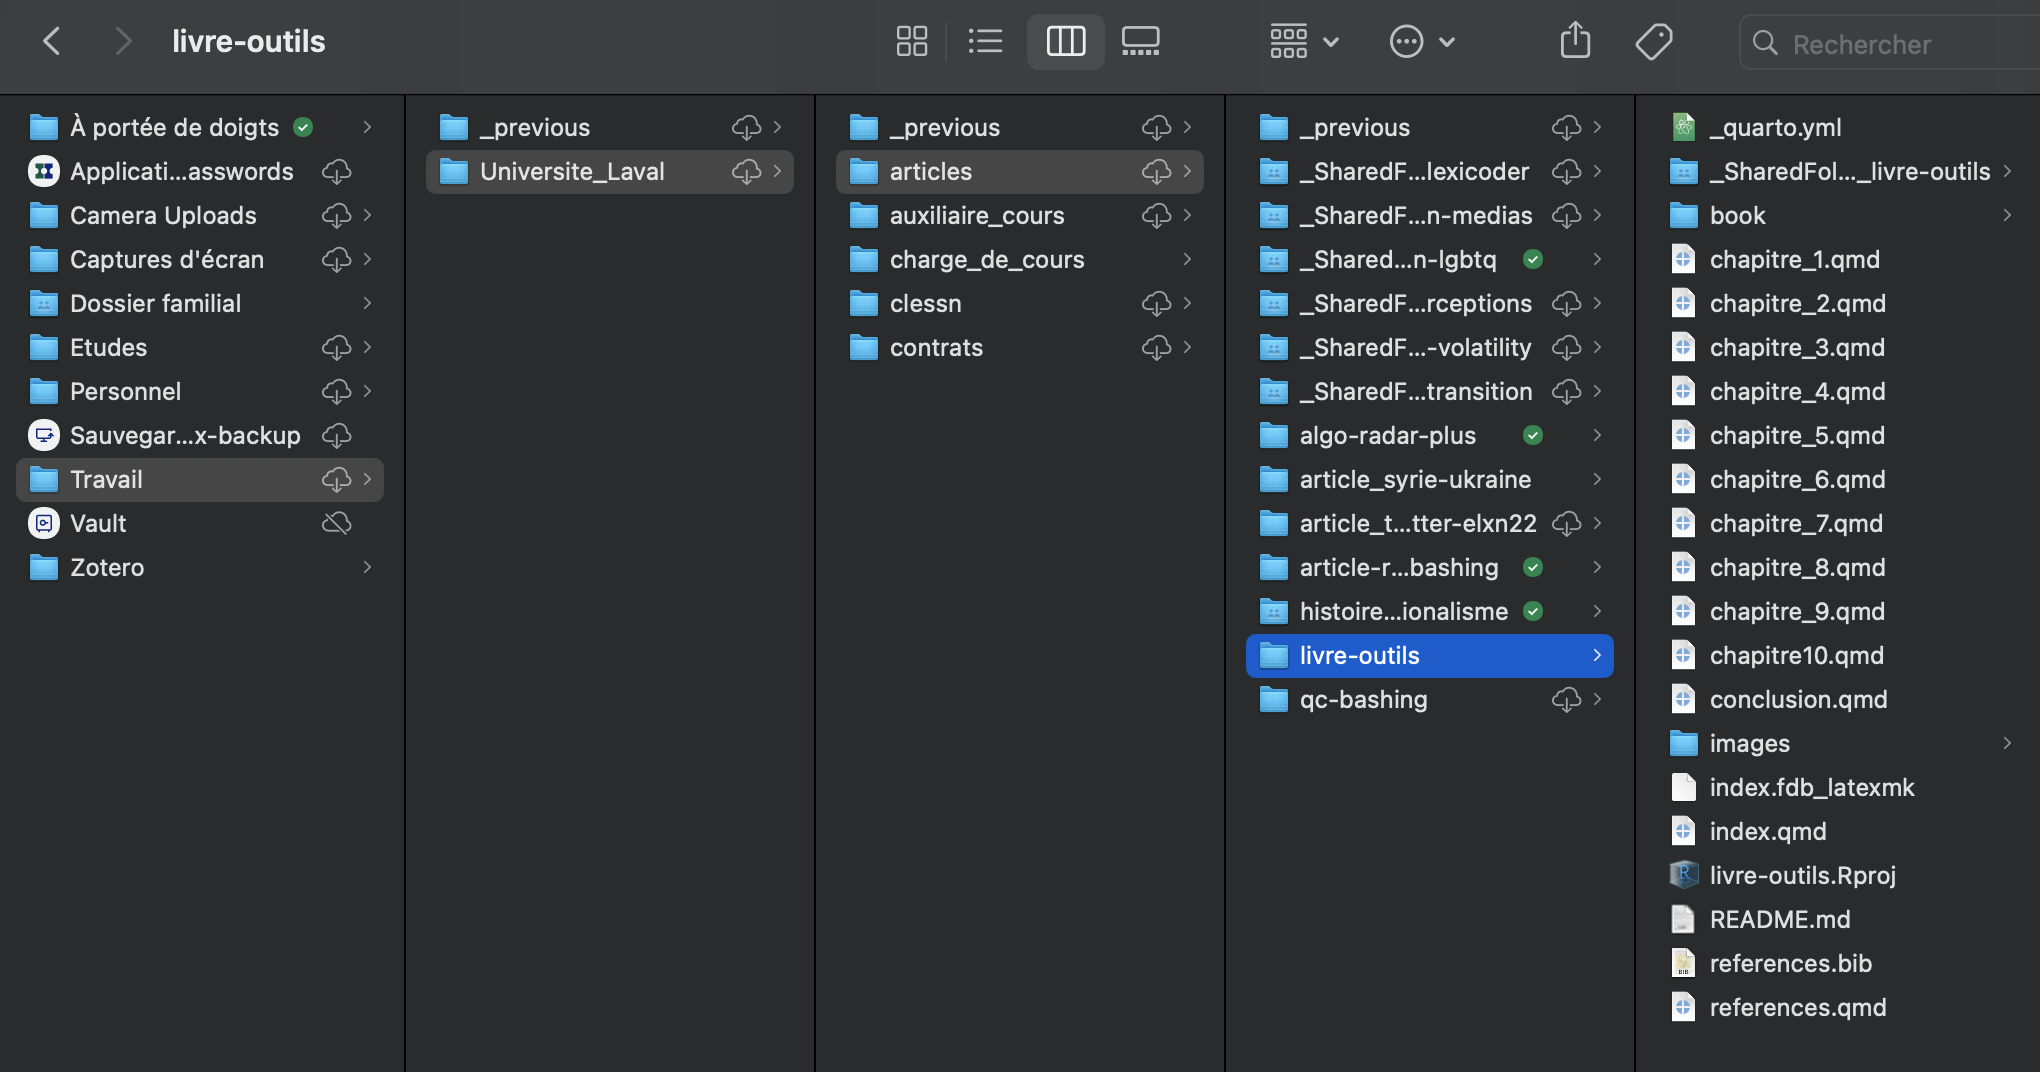
\includegraphics{images/chapitre8_dropbox.png}

}

\caption{image1}

\end{figure}%

Dropbox offre un suivi automatique des modifications, ce qui vous permet
de remonter dans le temps pour restaurer des versions antérieures de vos
fichiers. Cela garantit l'intégrité de vos données et vous permet de
revenir à des versions précédentes si nécessaire. De plus, l'archivage
de dossiers et de projets complets peut aider à conserver une vue
chronologique de votre travail au fil du temps.

Il est également crucial de considérer la taille de vos données. Si vous
traitez des fichiers volumineux tels que des images, des vidéos ou des
ensembles de données massifs, il peut être judicieux d'utiliser un
service cloud pour entreposer ces fichiers et les partager avec vos
collaborateurs, plutôt que de les pousser sur des plateformes de gestion
de versions comme GitHub.

Pour les données sensibles, les services cloud tels que Dropbox et
Google Drive peuvent ne pas être suffisamment sécurisés. C'est là que
des solutions comme AWS entrent en jeu. Cependant, il est important de
noter que l'utilisation d'AWS peut s'avérer complexe, en particulier
pour un jeune chercheur travaillant en solo ou en petite équipe.

\section{Gestion en équipe}\label{gestion-en-uxe9quipe}

\subsection{Coordination d'équipe (Slack
Mattermost)}\label{coordination-duxe9quipe-slack-mattermost}

Logiciel de gestion de communication (Slack)

Dans tout bon projet de recherche, la communication est primordiale. Que
ce soit pour décrire les avancements, discuter des étapes à venir,
entretenir un partenariat avec des partenaires ou simplement structurer
ses pensées, la plateforme par laquelle vous communiquez vous accompagne
à chacune des étapes du travail. Il est donc important de choisir un
outil qui convient bien à vos projets et de prendre le temps de
l'apprivoiser et d'optimiser son utilisation.

Il y a tellement de plateformes différentes pour communiquer qu'il faut
être prudent par rapport au nombre utilisé. Si vous ne faites pas un
choix, vous pouvez, sans vous en rendre compte, mêler Teams, courriels,
Zoom et autres. Rapidement, vous perdez le contrôle de ce qui est dit.
Nous vous proposons d'opter pour un logiciel de gestion de
communication. Il existe plusieurs logiciels du genre, tels que
Microsoft Teams, Slack, Google Workspace et Workplace. Toutes ces
options peuvent vous permettre de collaborer efficacement en équipe.
Dans le cadre de nos travaux, nous utilisons Slack. C'est donc
principalement de cet outil que nous parlerons dans cette section, mais
n'hésitez pas à vérifier quelle plateforme correspond le mieux à vos
besoins.

Peu importe votre niveau d'implication, la collaboration et la
communication sont inévitables en recherche. La science n'est pas une
discipline qui se développe en solitaire, elle nécessite des échanges et
des débats. Les équipes de recherche sont souvent dispersées
géographiquement. Même si vous travaillez actuellement seulement avec
votre directeur, il est certain que plusieurs équipes de recherche dans
votre département utilisent un tel logiciel. Un courriel peut faire
l'affaire pour une discussion ponctuelle qui se règle rapidement.
Cependant, dans une équipe de travail dynamique, où plusieurs membres
participent à divers projets, les courriels deviennent rapidement
chaotiques, il est difficile de retracer ce qui a été dit et de
conserver les pièces jointes. Les discussions deviennent rapidement trop
complexes pour le médium utilisé.

Les logiciels de gestion de communication ont été conçus spécifiquement
pour répondre aux besoins des équipes collaboratives. Vous y trouverez
leur facette la plus attrayante~: une structure simple et adaptée. Les
chaînes et fils de discussions permettent de garder des traces et de se
retrouver facilement dans ce qui a été dit. Une autre force de ces
logiciels est la centralisation des outils de travail. Sur Slack, comme
sur Teams, vous pouvez faire des appels en visioconférence à l'endroit
où vos conversations écrites se trouvent. Il est aussi possible d'y
télécharger l'application mobile, ce qui facilite l'accessibilité et la
connexion des membres de l'équipe. Tout avoir structuré à son goût au
même endroit et à portée de main, cela permet de structurer sa pensée
plus efficacement, d'éviter les oublis et de réduire le stress.

\subsubsection{Comment utiliser votre logiciel
efficacement}\label{comment-utiliser-votre-logiciel-efficacement}

Une fois que vous êtes convaincu d'aller de l'avant avec un de ces
outils, vous devrez apprendre à bien vous en servir. Voici quelques
trucs qui pourront vous aider à optimiser son utilisation. Les points
ci-dessous font référence à Slack, mais peuvent très bien être adaptés à
d'autres plateformes.

\subsubsection{Structuration}\label{structuration}

Il est important de bien réfléchir à la structuration de vos chaînes. Si
vous ne faites pas ce travail, les chaînes peuvent se multiplier
rapidement et les conversations se mettent alors à s'entrecroiser, vous
faisant ainsi perdre le fil. L'objectif de ces outils étant d'évitez ces
problèmes, vous ne voulez pas perdre l'avantage comparatif que vous
venez tout juste de gagner face aux courriels! La structuration des
chaînes devrait être similaire à celle de votre équipe de recherche. Si
vous utilisez Notion ou un autre logiciel du genre, la structure des
deux outils devrait être la même. Nous vous proposons d'avoir une chaîne
pour chacun des projets. Si le projet est trop gros et que la
conversation devient chaotique, pensez à créer une sous-chaîne (un
sous-projet) qui vous permettra d'aborder un sujet précis, sans mêler
les discussions. Pour faciliter la structuration des chaînes, vous
pouvez utiliser des préfixes, pour classer les chaînes par thème, ou
autre typologie qui vous convient. Également, utilisez les Espaces
d'équipe. Chaque équipe devrait avoir son propre espace, avec ses
propres chaînes. Vous pouvez faire partie de plusieurs équipes et
naviguer à travers les espaces. Si plusieurs équipes partagent un même
espace de travail, vous pourriez perdre le contrôle de sa structure.

\subsubsection{Maintenance}\label{maintenance}

Slack est un espace dynamique, tout comme votre équipe! La structure que
vous avez choisie n'est pas permanente. Vous devriez rapidement vous
questionner à savoir si elle convient toujours à vos activités. Votre
espace d'équipe est comme votre réel lieu de travail, faites-y
régulièrement le ménage pour vous assurer que tout est propre et en
ordre. Archivez les chaînes qui ne sont plus pertinentes ou actives,
puisque vous pourrez toujours les désarchiver quand cela sera
nécessaire. Épinglez des messages importants et des documents utiles aux
projets dans les chaînes appropriées. Faites le tour de ce qui est
épinglé à l'occasion pour vérifier si c'est encore pertinent. Cela peut
paraître énergivore, mais l'efficacité de votre travail d'équipe va en
bénéficier. Également, rappelez aux membres de votre équipe d'utiliser
les bonnes chaînes pour chacune des discussions. Il ne faut pas que les
conversations se croisent à travers les chaînes. Chaque chaîne a son
utilité et doit être utilisée en conséquence. Les appels d'équipe
doivent aussi se faire dans les bonnes chaînes. Quand vous êtes en
appel, utilisez le fil de discussion pour conserver des traces écrites
des points abordés dans la réunion. Les fils de discussions sont en
général un bon outil pour ne pas se perdre dans un discussion. Si
l'usage des mauvaises chaînes est un problème récurent, il est possible
que la structure que vous employez est mal adaptée à vos travaux. Vous
pouvez alors retourner à la planche à dessin. Assurez-vous que toute
l'équipe comprenne bien comment utiliser Slack. Si ce n'est pas le cas,
formez-les. Une structure adaptée et une équipe bien formée peuvent
faire des miracles.

\subsubsection{Collaboration}\label{collaboration}

La grande majorité des conversations devraient se faire dans les
chaînes. Les conversations privées ont leur utilité, vous vous en
servirez. Il est parfois nécessaire d'avoir des discussions plus
confidentielles et de parler rapidement à quelqu'un sur un sujet
éphémère. Toutefois, par soucis de transparence et d'inclusion, toute
discussion à propos d'un projet devrait se faire dans sa chaîne. Si vous
jugez qu'un membre d'une chaîne ne devrait pas lire ce que vous avez à
dire sur le projet, c'est qu'il ne devrait pas faire partie de la
chaîne. Par rapport aux membres, trouvez le bon équilibre par rapport à
qui devrait être dans quelle chaîne. L'objectif n'est pas d'exclure et
de cacher du contenu, vous voulez une équipe transparente. Vous voulez
que vos membres restent bien informés de l'avancement des projets sans
les submerger d'information qui ne leur est pas utile. C'est à vous de
trouver la formule gagnante. Invitez vos partenaires externes dans votre
espace d'équipe. Créez des chaînes spécifiques aux partenaires pour que
les conversations externes soient tout aussi organisées. N'invitez pas
vos partenaires dans vos chaînes privées, question de confidentialité.
Si un partenaire n'a pas l'habitude d'utiliser Slack ou l'outil que vous
utilisez, proposez-lui de vous y joindre quand même. Moins vous utilisez
les outils des autres, plus vous gardez centralisées vos communications
et évitez de jongler avec plusieurs plateformes.

\subsubsection{Optimisation personnelle}\label{optimisation-personnelle}

Une fois que la structure d'équipe est définie et que vos membres et vos
partenaires sont à l'aise avec l'utilisation de la plateforme, il est
temps d'organiser la structure de votre Slack personnel. Créez des
sections pour trier les chaînes. La structure d'équipe est essentielle,
mais une fois qu'elle est déterminée, chaque membre n'utilise pas
forcément les chaînes de la même façon. Vous pouvez vous créer une
section de favoris, ou encore différentes sections par rapport aux
différents thèmes pour y faciliter la navigation. Également, ajustez vos
paramètres de notifications. C'est à vous de déterminer quelle chaînes
méritent de produire des alertes, et à quels moments vous souhaitez les
recevoir. Slack a plusieurs applications intégrées qui facilitent la
compatibilité avec vos autres outils. Vous pouvez connecter votre
calendrier, votre Notion et votre GitHub pour recevoir des alertes
pertinentes. Allez explorer ces applications pour déterminer lesquelles
vous conviennent.

Tel que mentionné précédemment, plusieurs logiciels peuvent convenir à
vos besoins. Puisque nous utilisons Slack, voici quelques raisons qui
pourraient vous convaincre d'opter pour cette option ou de vous en
éloigner. Sachez que cette liste n'est pas du tout exhaustive, mais
reflète simplement quelques-unes de nos observations par rapport à notre
outil de travail.

\begin{itemize}
\item
  Avantages

  L'utilisation de Slack est très intuitive. Nous l'utilisons
  régulièrement dans des cours, et les étudiants apprennent rapidement à
  l'utiliser. La distinction entre les chaînes publiques accessibles à
  tous les membres d'un espace d'équipe et les chaînes privées est
  claire et simple d'utilisation. Slack offre aussi une fonction de
  recherche, qui vous permet de retrouver des messages à travers les
  chaînes. L'intégration de applications qui font le pont avec d'autres
  outils est fort appréciée. Enfin, Slack est utilisé partout dans le
  monde par des équipes de toutes les tailles et dans tous les domaines.
  C'est un outil très présent en recherche académique qui facilite la
  collaboration et la multidisciplinarité. Les chances sont élevées que
  vos partenaires utilisent déjà l'outil, ou au minimum en aient déjà
  entendu parlé.
\item
  Inconvénients

  Si vous avez l'habitude d'utiliser les outils d'une suite, comme
  celles de Microsoft ou de Google, il est possible que vous trouviez
  l'intégration de ces outils à Slack moins pratique que si vous
  utilisiez les plateformes proposées par ces compagnies. Également,
  gardez en tête que la version gratuite de Slack a plusieurs
  limitations. Elle implique notamment un limite de temps par rapport à
  l'archivage des messages, que vous ne pourrez pas retracer après 90
  jours. Les coûts pour utiliser Slack à son plein potentiel peuvent
  être élevés, mais puisque ce genre d'outils est de plus en plus
  répandu, il est fort possible que son utilisation soit financée par
  votre département.
\end{itemize}

\subsection{Gestion de tâches en équipe (Notion,
Monday)}\label{gestion-de-tuxe2ches-en-uxe9quipe-notion-monday}

\subsection{Gestion de versions en équipe (Pull-push,
pull-requests)}\label{gestion-de-versions-en-uxe9quipe-pull-push-pull-requests}

Lorsque l'on aborde le domaine de la recherche scientifique en sciences
sociales numériques, la collaboration et la gestion efficace du code
deviennent des éléments cruciaux pour progresser dans ses projets. Dans
cette optique, les outils de gestion de versions décentralisés ont pris
une place prépondérante. Parmi eux, Git et GitHub se démarquent tant par
leur popularité que par leur efficacité.

\subsubsection{Avantages}\label{avantages}

Git, développé par Linus Torvalds en 2005, s'est imposé comme le système
de gestion de versions décentralisé de référence. Sa principale force
réside dans sa capacité à suivre l'évolution d'un projet en enregistrant
les modifications apportées au code source. Chaque modification est
enregistrée sous forme de dépôts (\emph{commits}), avec un message
explicatif, permettant aux collaborateurs de comprendre facilement les
évolutions du projet.

GitHub, lancé en 2008, est une plateforme qui utilise Git comme base
pour l'entreposage et la gestion de projets. C'est une vitrine virtuelle
où les développeurs peuvent héberger leurs dépôts Git et collaborer de
manière transparente. L'aspect social de GitHub, avec ses
fonctionnalités de suivi des projets, de gestion des problèmes et de
demandes de fusion, en fait un lieu de choix pour les projets en code
source ouvert et collaboratifs.

En sciences sociales numériques, où le partage et la collaboration sont
essentiels, Git et GitHub offrent plusieurs avantages majeurs. Tout
d'abord, ils permettent de suivre les modifications apportées au code,
ce qui facilite la reproductibilité des résultats. Les chercheurs
peuvent revenir à n'importe quelle version précédente du code, ce qui
est particulièrement utile pour corriger des erreurs ou analyser
l'impact de différentes approches.

De plus, Git et GitHub favorisent le travail collaboratif. Plusieurs
chercheurs peuvent travailler sur le même projet simultanément, chacun
dans sa branche de développement. Une fois les modifications effectuées,
il est possible de fusionner les branches pour intégrer les changements.
Cette approche évite les conflits majeurs et facilite la répartition des
tâches au sein de l'équipe.

Enfin, l'aspect de code source ouvert de GitHub permet aux chercheurs en
sciences sociales numériques de partager leurs codes avec la communauté
académique et de bénéficier des contributions d'autres chercheurs. Cela
favorise un environnement de partage des connaissances et de
collaboration fructueuse.

\subsubsection{Inconvénients}\label{inconvuxe9nients}

Cependant, Git et GitHub ne sont pas sans leurs défis. La courbe
d'apprentissage peut être raide pour les débutants, car ces outils
impliquent des concepts spécifiques tels que les branches, les conflits
de fusion et les requêtes de tirage. De plus, bien que GitHub offre un
niveau de gratuité pour les projets en code source ouvert, des frais
peuvent être appliqués pour des fonctionnalités avancées ou pour des
projets privés.

\subsubsection{Comment les utiliser efficacement (en parallèle à
Dropbox,
etc.)}\label{comment-les-utiliser-efficacement-en-paralluxe8le-uxe0-dropbox-etc.}

Pour utiliser Git et GitHub efficacement dans un contexte de recherche
en sciences sociales numériques, il est recommandé de suivre quelques
bonnes pratiques. Tout d'abord, il est important de structurer son dépôt
Git de manière logique, en organisant les fichiers et les dossiers de
manière cohérente. Les messages de commit doivent être descriptifs et
clairs, pour permettre à tous les collaborateurs de comprendre les
changements effectués.

Il est également conseillé de travailler sur des branches distinctes
pour chaque fonctionnalité ou modification majeure. Cela facilite la
gestion des changements et minimise les conflits lors de la fusion. Les
chercheurs devraient également consulter régulièrement les projets et
les problèmes sur GitHub pour encourager une communication ouverte et
résoudre rapidement les problèmes.

L'utilisation de Git et de GitHub peut être complémentaire à d'autres
outils d'entreposage, tels que Dropbox ou Google Drive. Ces derniers
peuvent être utilisés pour entreposer des fichiers non liés au code,
tels que des données brutes non sensibles ou des documents de recherche,
tandis que Git et GitHub gèrent le code source et ses évolutions.

Bien qu'il existe plusieurs alternatives à l'utilisation combinée de Git
et de GitHub sur le marché, ces deux plateformes liées continuent de
dominer le domaine de la gestion de versions décentralisée. Parmi les
alternatives notables, on peut citer Mercurial, Bitbucket, GitLab et
SourceForge. Chacun de ces outils offre des fonctionnalités similaires à
celles de Git et GitHub, mais il est important de comprendre pourquoi
Git et GitHub restent les choix privilégiés pour les chercheurs en
sciences sociales numériques.

\subsubsection{Pourquoi prioriser Git et GitHub pour les chercheurs en
sciences
sociales}\label{pourquoi-prioriser-git-et-github-pour-les-chercheurs-en-sciences-sociales}

\begin{enumerate}
\def\labelenumi{\arabic{enumi}.}
\item
  \emph{Intégration et adoption répandue}~: Git est devenu un standard
  de facto dans l'industrie du développement logiciel. Sa popularité et
  son adoption répandue signifient que de nombreuses ressources
  d'apprentissage, des tutoriels et des forums de support sont
  disponibles en ligne, ce qui facilite l'utilisation de cet outil pour
  les chercheurs en sciences sociales débutants. GitHub, en tant que
  plateforme principale de gestion des versions, bénéficie également
  d'une grande base d'utilisateurs et d'une communauté active, ce qui
  encourage la collaboration et le partage des connaissances.
\item
  \emph{Facilité de collaboration}~: Git et GitHub sont conçus pour
  faciliter la collaboration entre les individus et les équipes. Les
  chercheurs en sciences sociales travaillent souvent ensemble sur des
  projets de recherche, et la capacité de suivre les modifications, de
  gérer les conflits et de fusionner les contributions devient
  essentielle. L'interface conviviale de GitHub, avec des
  fonctionnalités telles que les demandes de fusion et les commentaires
  en ligne, simplifie grandement la collaboration.
\item
  \emph{Visibilité et partage}~: GitHub brille par sa fonctionnalité de
  projet open source, qui permet aux chercheurs en sciences sociales de
  partager leurs travaux avec la communauté mondiale. Les projets en
  code source ouvert sont visibles et accessibles à tous, favorisant
  ainsi la collaboration et l'examen par les pairs. Cela peut être
  particulièrement bénéfique pour les chercheurs souhaitant contribuer à
  des initiatives académiques et collaborer à des projets
  interdisciplinaires.
\item
  \emph{Suivi des versions et recherche reproductible}~: Les chercheurs
  en sciences sociales doivent s'assurer que leurs travaux sont
  reproductibles et vérifiables. Git permet de suivre les versions du
  code, ce qui signifie que les chercheurs peuvent retrouver facilement
  des versions antérieures pour reproduire des analyses spécifiques ou
  corriger des erreurs. Cette fonctionnalité est cruciale pour maintenir
  l'intégrité des résultats de recherche.
\item
  \emph{Infrastructure et sécurité}~: GitHub offre une infrastructure
  robuste pour l'entreposage sécurisé des dépôts Git. Les chercheurs
  peuvent être assurés que leurs travaux sont sauvegardés et protégés
  contre les pertes de données accidentelles. De plus, les contrôles
  d'accès et les autorisations granulaires de GitHub permettent aux
  chercheurs de contrôler qui peut accéder et contribuer à leurs
  projets.
\end{enumerate}

En somme, Git et GitHub offrent aux chercheurs en sciences sociales
numériques un moyen puissant de gérer leur code, de collaborer
efficacement et de contribuer à la communauté académique grâce à l'open
source. Bien que leur apprentissage puisse représenter un défi initial,
les avantages qu'ils apportent en termes de suivi des versions, de
collaboration et de partage des connaissances en font des outils
essentiels dans l'arsenal de tout chercheur moderne.

\subsubsection{Pratiques à éviter sur GitHub pour les chercheurs en
sciences
sociales}\label{pratiques-uxe0-uxe9viter-sur-github-pour-les-chercheurs-en-sciences-sociales}

Lorsque les chercheurs en sciences sociales utilisent GitHub pour
partager leur code, collaborer sur des projets et contribuer à la
communauté académique, il est essentiel de connaître les pratiques à
éviter. En effet, certaines erreurs peuvent compromettre la sécurité, la
confidentialité et l'efficacité de la recherche. Voici quelques éléments
à éviter~:

\begin{enumerate}
\def\labelenumi{\arabic{enumi}.}
\item
  \emph{Entreposer des informations sensibles}~: Évitez d'entreposer des
  données sensibles ou confidentielles sur GitHub. Cela inclut les
  données de sondages, les informations personnelles identifiables et
  tout autre contenu pouvant porter atteinte à la vie privée des
  individus. Assurez-vous de supprimer ou de masquer soigneusement ces
  informations avant de les télécharger sur la plateforme.
\item
  \emph{Inclure des mots de passe et clés d'accès}~: Ne jamais inclure
  de mots de passe, de clés d'accès ou d'informations d'identification
  dans votre code source. Cela peut compromettre la sécurité de vos
  systèmes et de vos données. Utilisez plutôt des méthodes sécurisées
  pour gérer ces informations, telles que les variables d'environnement
  ou les fichiers de configuration externes.
\item
  \emph{Entreposer des fichiers lourds}~: Évitez d'entreposer des
  fichiers volumineux sur GitHub, notamment des fichiers binaires, des
  données brutes massives ou des ensembles de données volumineux. Ces
  fichiers peuvent ralentir les opérations de clonage et de fusion, ce
  qui affecte la performance globale du dépôt. Utilisez plutôt des
  services d'entreposage dédiés pour ces fichiers et fournissez des
  liens vers ces ressources dans votre dépôt.
\item
  \emph{Inclure des identifiants personnels}~: Évitez de publier vos
  propres identifiants personnels, tels que des numéros de sécurité
  sociale, des numéros de carte de crédit ou d'autres informations
  confidentielles. Ces informations pourraient être exploitées à des
  fins malveillantes si elles tombent entre de mauvaises mains.
\item
  \emph{Ignorer les pratiques de branches et de fusion}~: Évitez de
  fusionner directement du code dans la branche principale
  (habituellement appelée \emph{main} ou \emph{master}). Utilisez plutôt
  des branches distinctes pour les fonctionnalités et les corrections,
  et suivez les pratiques de fusion pour intégrer proprement les
  changements. Ignorer ces pratiques peut entraîner des conflits et une
  perte de trace des modifications.
\item
  \emph{Ignorer les commentaires des collaborateurs}~: Lorsque vous
  travaillez avec d'autres chercheurs, ne négligez pas les commentaires
  et les suggestions qu'ils fournissent. Les retours d'expérience et les
  idées des autres peuvent contribuer à améliorer la qualité de votre
  code et de vos analyses.
\item
  \emph{Ne pas documenter}~: Évitez de ne pas documenter votre code. Une
  documentation claire et détaillée est essentielle pour permettre à
  d'autres chercheurs de comprendre vos méthodes et vos résultats.
  Utilisez des commentaires explicatifs et fournissez des explications
  sur la manière d'exécuter votre code.
\end{enumerate}

En suivant ces conseils et en évitant ces erreurs courantes, les
chercheurs en sciences sociales peuvent garantir la sécurité, la qualité
et l'efficacité de leurs projets sur GitHub. La responsabilité de
préserver la confidentialité des données et de créer un environnement de
travail collaboratif et respectueux repose sur les épaules de chaque
contributeur.

\subsubsection{Exemple d'utilisation de Git et de GitHub pour un
chercheur en sciences
sociales}\label{exemple-dutilisation-de-git-et-de-github-pour-un-chercheur-en-sciences-sociales}

Dans le contexte de la recherche en sciences sociales numériques, la
gestion efficace du code, la collaboration transparente et la
préservation des données sensibles sont des impératifs. Imaginons que
vous êtes un jeune chercheur en sciences sociales qui étudie l'impact
des médias sur l'opinion publique. Vous utilisez le langage de
programmation R pour analyser des données de médias et des données de
sondage. Bien que vous travailliez seul, vous souhaitez rendre votre
travail accessible à votre équipe pour validation et permettre à vos
collègues de contribuer aux améliorations. Voici comment vous pouvez
utiliser Git et GitHub pour gérer votre projet de manière structurée et
collaborative.

\paragraph{Étape 1~: Création d'un répertoire local et initialisation de
Git}\label{uxe9tape-1-cruxe9ation-dun-ruxe9pertoire-local-et-initialisation-de-git}

Ouvrez votre terminal et naviguez vers le dossier où vous souhaitez
enregistrer votre projet.

\begin{Shaded}
\begin{Highlighting}[]
\BuiltInTok{cd}\NormalTok{ chemin/vers/votre/dossier}
\end{Highlighting}
\end{Shaded}

Créez un nouveau répertoire pour votre projet et accédez-y.

\begin{Shaded}
\begin{Highlighting}[]
\FunctionTok{mkdir}\NormalTok{ mon\_projet}
\end{Highlighting}
\end{Shaded}

\begin{Shaded}
\begin{Highlighting}[]
\BuiltInTok{cd}\NormalTok{ mon\_projet}
\end{Highlighting}
\end{Shaded}

Initialisez Git dans ce répertoire.

\begin{Shaded}
\begin{Highlighting}[]
\FunctionTok{git}\NormalTok{ init}
\end{Highlighting}
\end{Shaded}

\paragraph{Étape 2~: Ajout de votre code et de vos
fichiers}\label{uxe9tape-2-ajout-de-votre-code-et-de-vos-fichiers}

Ajoutez vos fichiers R contenant le code pour l'analyse des médias et
des sondages dans le répertoire. Par exemple, vous pouvez avoir des
fichiers \emph{analyse\_medias.R} et \emph{analyse\_sondages.R}.

Utilisez la commande \texttt{git\ status} pour vérifier l'état de vos
fichiers.

\begin{Shaded}
\begin{Highlighting}[]
\FunctionTok{git}\NormalTok{ status}
\end{Highlighting}
\end{Shaded}

\paragraph{Étape 3~: Ajout, validation et commit de vos
modifications}\label{uxe9tape-3-ajout-validation-et-commit-de-vos-modifications}

Ajoutez vos fichiers pour qu'ils soient prêts à être validés.

\begin{Shaded}
\begin{Highlighting}[]
\FunctionTok{git}\NormalTok{ add }\AttributeTok{{-}A}
\end{Highlighting}
\end{Shaded}

Validez vos modifications avec un message descriptif.

\begin{Shaded}
\begin{Highlighting}[]
\FunctionTok{git}\NormalTok{ commit }\AttributeTok{{-}m} \StringTok{"Ajout du code d\textquotesingle{}analyse des médias et des sondages"}
\end{Highlighting}
\end{Shaded}

\paragraph{Étape 4~: Création du répertoire sur GitHub et du lien avec
votre répertoire
local}\label{uxe9tape-4-cruxe9ation-du-ruxe9pertoire-sur-github-et-du-lien-avec-votre-ruxe9pertoire-local}

Allez sur GitHub et connectez-vous à votre compte. Créez un nouveau
répertoire vide avec le nom \emph{mon\_projet}.

De retour dans votre terminal, ajoutez le lien GitHub à votre répertoire
local.

\begin{Shaded}
\begin{Highlighting}[]
\FunctionTok{git}\NormalTok{ remote add origin https://github.com/votre{-}utilisateur/mon\_projet.git}
\end{Highlighting}
\end{Shaded}

\paragraph{Étape 5~: Push de votre travail sur
GitHub}\label{uxe9tape-5-push-de-votre-travail-sur-github}

Envoyez vos commits locaux vers GitHub.

\begin{Shaded}
\begin{Highlighting}[]
\FunctionTok{git}\NormalTok{ push }\AttributeTok{{-}u}\NormalTok{ origin master}
\end{Highlighting}
\end{Shaded}

\paragraph{Étape 6~: Collaboration avec vos
collègues}\label{uxe9tape-6-collaboration-avec-vos-colluxe8gues}

Si vos collègues souhaitent contribuer à votre projet, ils peuvent
\emph{forker} votre répertoire sur GitHub, ce qui créera une copie dans
leur propre compte.

Lorsqu'ils ont fait des modifications dans leur copie, ils peuvent
soumettre une \emph{pull request} pour vous demander de fusionner leurs
modifications dans votre répertoire principal.

\paragraph{Étape 7~: Pull des modifications de vos
collègues}\label{uxe9tape-7-pull-des-modifications-de-vos-colluxe8gues}

Lorsque vos collègues ont soumis des modifications et vous ont demandé
de les fusionner, vous pouvez mettre à jour votre répertoire local avec
leurs changements.

\begin{Shaded}
\begin{Highlighting}[]
\FunctionTok{git}\NormalTok{ pull origin master}
\end{Highlighting}
\end{Shaded}

\paragraph{Étape 8~: Répéter le
processus}\label{uxe9tape-8-ruxe9puxe9ter-le-processus}

Répétez les étapes 2 à 7 au fur et à mesure que vous développez votre
projet, ajoutez du code, effectuez des analyses et collaborez avec vos
collègues. Assurez-vous de valider et de pousser régulièrement vos
modifications pour maintenir le dépôt à jour.

\subsubsection{GitHub Desktop}\label{github-desktop}

Alors que le terminal reste une approche fondamentale pour maîtriser Git
et GitHub, il existe des outils conviviaux tels que GitHub Desktop qui
offrent une alternative intuitive. Cet outil simplifie le processus de
gestion de versions décentralisée, en particulier pour ceux qui
souhaitent commencer par une approche visuelle. Cependant, comprendre
son fonctionnement et équilibrer les avantages et les inconvénients est
essentiel.

\begin{figure}[H]

{\centering 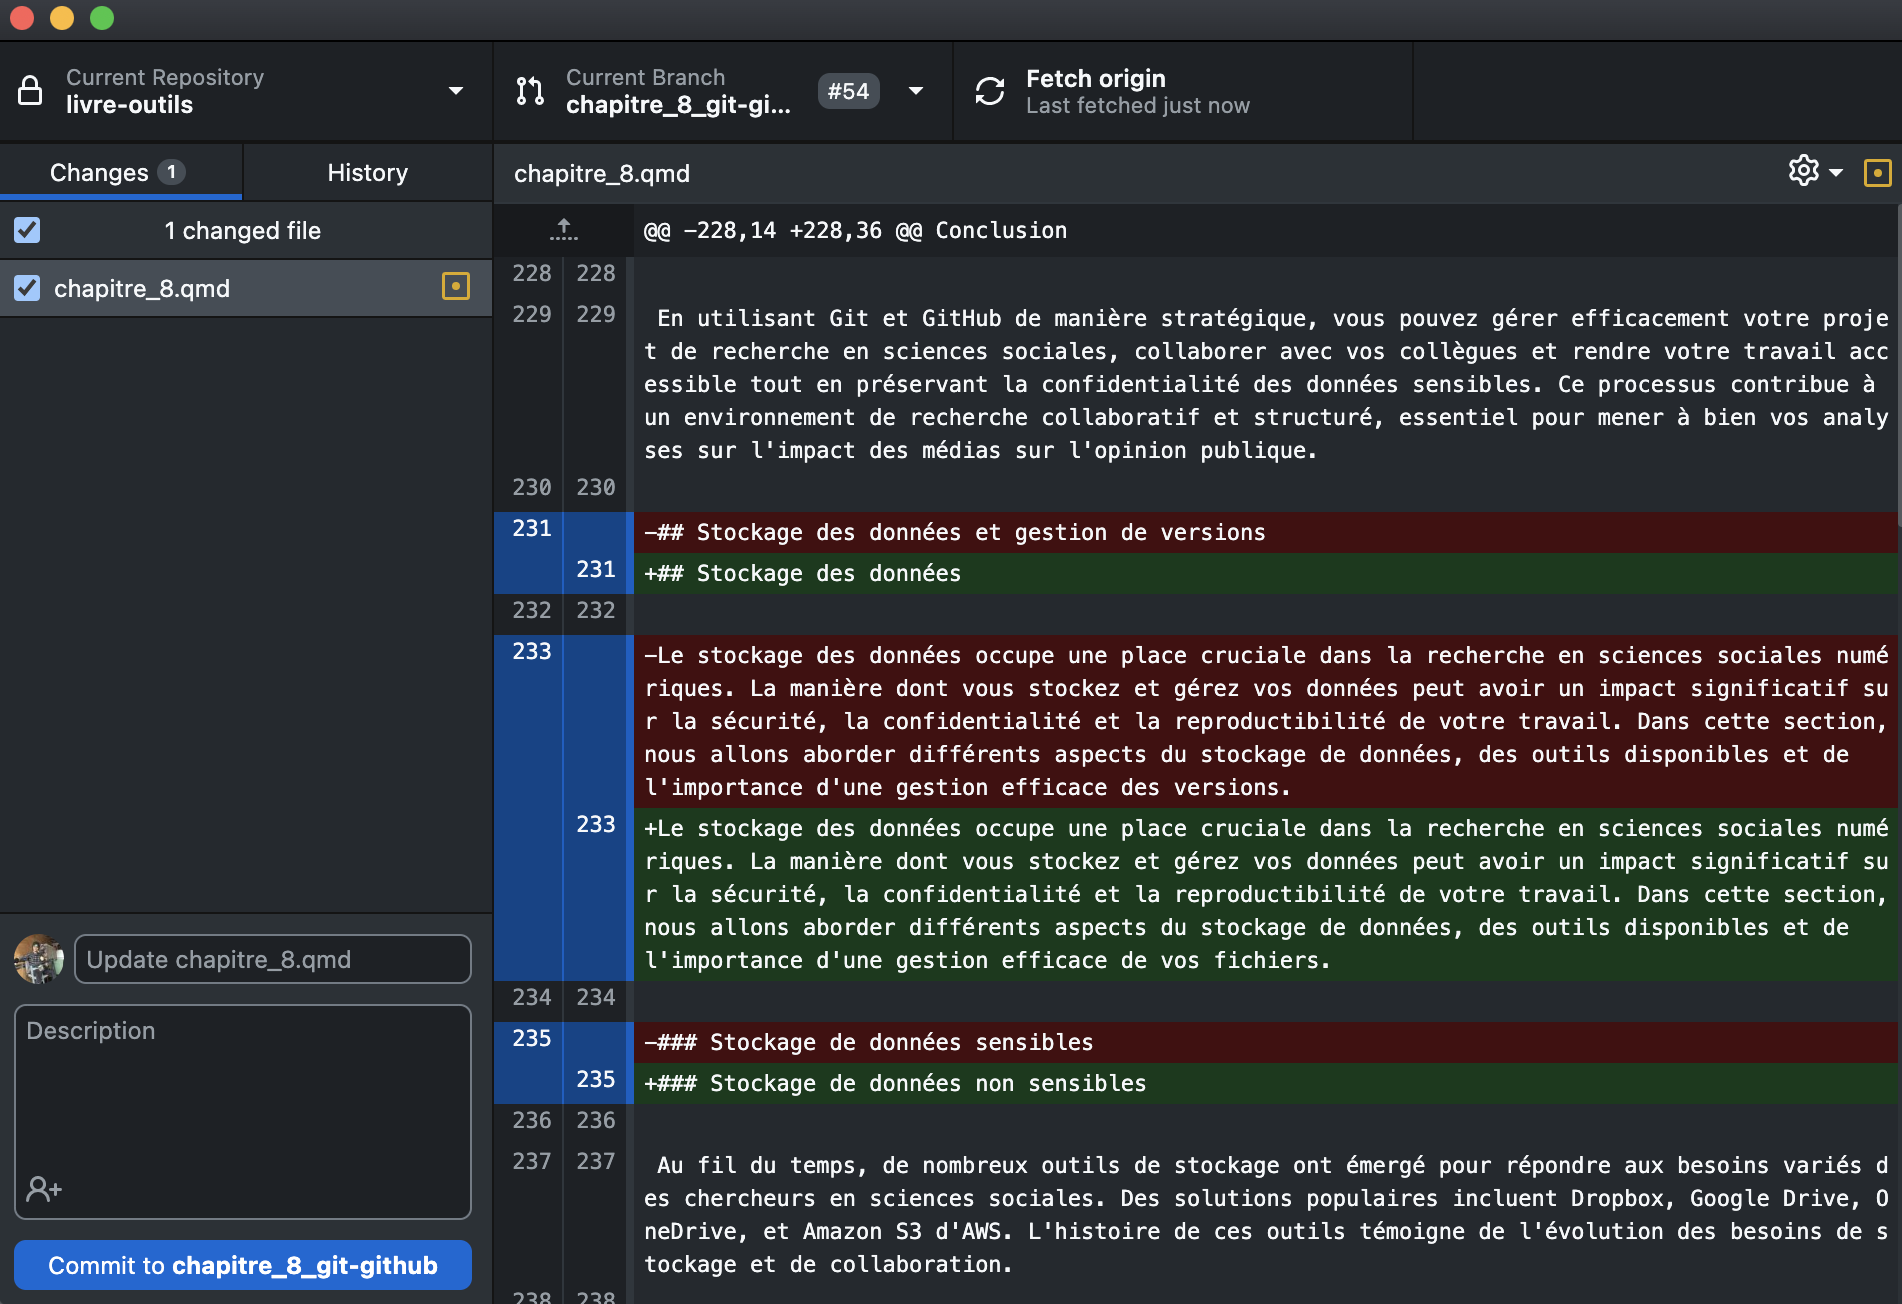
\includegraphics{images/chapitre8_gitdesktop.png}

}

\caption{image}

\end{figure}%

GitHub Desktop fournit une vue claire de vos dépôts, de vos
modifications, de vos branches et de vos demandes de fusion. Il élimine
la nécessité de mémoriser les commandes en ligne de terminal, ce qui
peut être un défi pour certains chercheurs. L'application simplifie
également la résolution des conflits lors de la fusion des branches.

Toutefois, en utilisant GitHub Desktop, il est possible de perdre la
compréhension des commandes Git en ligne de commande, ce qui pourrait
devenir un inconvénient si vous devez travailler dans un environnement
sans interface visuelle. De plus, GitHub Desktop est spécifiquement
conçu pour interagir avec GitHub. Si vous devez travailler avec d'autres
plateformes de gestion de versions, cela pourrait poser des problèmes.

La décision entre l'utilisation du terminal et de GitHub Desktop dépend
de vos préférences et de vos besoins. Pour les chercheurs qui débutent,
GitHub Desktop offre une transition en douceur vers les concepts de
gestion de versions. Cependant, il est important de ne pas se limiter à
une interface visuelle. Comprendre les commandes Git en ligne de
commande reste essentiel pour résoudre des problèmes complexes, gérer
des projets avancés et collaborer avec d'autres chercheurs qui utilisent
des approches basées sur le terminal.

\subsubsection{Conclusion}\label{conclusion-2}

En utilisant Git et GitHub de manière stratégique, vous pouvez gérer
efficacement votre projet de recherche en sciences sociales, collaborer
avec vos collègues et rendre votre travail accessible tout en préservant
la confidentialité des données sensibles. Ce processus contribue à un
environnement de recherche collaboratif et structuré, essentiel pour
mener à bien vos analyses sur l'impact des médias sur l'opinion
publique.

\#\#Stockage de données (AWS, Valeria)

\subsection{Entreposage de données
sensibles}\label{entreposage-de-donnuxe9es-sensibles}

Lorsqu'il s'agit d'entreposer des données sensibles, tels que des
données de sondage comportant des informations personnelles
identifiables, la sécurité et la confidentialité sont essentielles.
Comme abordé précédemment, GitHub n'est pas adapté à l'entreposage de
telles données en raison de ses caractéristiques publiques et de son
orientation vers le code source ouvert. Une solution courante est
d'utiliser des services de cloud sécurisés, tels qu'AWS, qui offrent des
mesures de sécurité robustes pour protéger vos données sensibles.

AWS regroupe un ensemble de services \emph{cloud} proposés par Amazon.
Il offre une vaste gamme de services, allant de l'entreposage et de la
gestion des données à la computation et à l'analyse avancée. AWS est
conçu pour offrir une infrastructure hautement évolutive et sécurisée,
ce qui en fait un choix attrayant pour les chercheurs qui gèrent des
données sensibles. L'outil présente de multiples avantages:

\begin{enumerate}
\def\labelenumi{\arabic{enumi}.}
\item
  \emph{Sécurité robuste}~: AWS met l'accent sur la sécurité, avec des
  fonctionnalités telles que le chiffrement des données en transit et au
  repos, la gestion des accès basée sur les rôles et la conformité à des
  normes de sécurité strictes.
\item
  \emph{Scalabilité}~: AWS permet de faire évoluer vos ressources en
  fonction des besoins, garantissant des performances optimales même
  lorsque vos projets de recherche croissent en taille et en complexité.
\item
  \emph{Flexibilité}~: AWS propose une variété de services adaptés à
  différentes utilisations, allant de l'entreposage de données au calcul
  intensif pour l'analyse avancée.
\item
  \emph{Collaboration simplifiée}~: Bien que le coût d'entrée soit
  généralement bas, la possibilité de partager des ressources avec des
  collègues et de travailler en équipe rend AWS adapté à la
  collaboration.
\end{enumerate}

AWS n'est pas le seul service cloud disponible. Microsoft Azure et
Google Cloud Platform (GCP) sont des concurrents majeurs offrant des
fonctionnalités similaires. Lorsque vous choisissez un fournisseur,
prenez en compte les coûts, la convivialité et les fonctionnalités
offertes. Le coût d'utilisation d'AWS peut varier en fonction des
services utilisés, de la quantité de données entreposées et de la
capacité de calcul requise. Lorsque vous travaillez seul, le coût peut
sembler élevé par rapport à l'utilisation de solutions gratuites telles
que Dropbox. Cependant, en équipe, la répartition des coûts peut rendre
AWS plus abordable.

\subsubsection{Exemple d'utilisation d'AWS pour entreposer et accéder à
des données de sondages dans
RStudio}\label{exemple-dutilisation-daws-pour-entreposer-et-accuxe9der-uxe0-des-donnuxe9es-de-sondages-dans-rstudio}

Imaginez un jeune chercheur en sciences sociales qui travaille sur une
analyse comparative de données de sondages recueillies sur plusieurs
décennies. Pour maintenir la sécurité des données sensibles et faciliter
l'accès pour les analyses dans RStudio, il décide d'utiliser AWS pour
l'entreposage et la gestion de ses données.

\paragraph{Étape 1~: Création d'un compte AWS et
configuration}\label{uxe9tape-1-cruxe9ation-dun-compte-aws-et-configuration}

Le chercheur crée un compte AWS et configure ses paramètres de sécurité,
y compris la configuration de l'authentification à deux facteurs pour
renforcer la sécurité de son compte.

\paragraph{Étape 2~: Création d'un espace d'entreposage
S3}\label{uxe9tape-2-cruxe9ation-dun-espace-dentreposage-s3}

Le chercheur crée un compartiment Amazon S3 (Simple Storage Service)
pour entreposer ses données de sondage. Il choisit une région AWS et
définit les paramètres de sécurité appropriés, tels que le chiffrement
des données.

\paragraph{Étape 3~: Transfert des données vers Amazon
S3}\label{uxe9tape-3-transfert-des-donnuxe9es-vers-amazon-s3}

Le chercheur transfère les données de sondage dans son compartiment
Amazon S3 à l'aide de l'interface en ligne AWS ou d'outils
d'importation.

\paragraph{Étape 4~: Configuration des
autorisations}\label{uxe9tape-4-configuration-des-autorisations}

Pour sécuriser davantage les données, le chercheur configure les
autorisations d'accès aux données dans Amazon S3. Il attribue des rôles
et des politiques d'accès spécifiques aux utilisateurs, garantissant que
seules les personnes autorisées peuvent accéder aux données.

\paragraph{Étape 5~: Configuration d'accès dans
RStudio}\label{uxe9tape-5-configuration-daccuxe8s-dans-rstudio}

Le chercheur installe le package \emph{aws.s3} dans RStudio pour accéder
à ses données entreposées dans Amazon S3. Il configure également les
informations d'identification AWS dans son environnement RStudio.

\paragraph{Étape 6~: Accès et analyse des données dans
RStudio}\label{uxe9tape-6-accuxe8s-et-analyse-des-donnuxe9es-dans-rstudio}

À l'aide du package \emph{aws.s3}, le chercheur peut maintenant accéder
à ses données directement dans RStudio par quelques lignes de code. Il
peut charger les données dans des structures de données R et effectuer
des analyses statistiques, des visualisations et des croisements.

\paragraph{Étape 7~: Sécurité et conservation des
données}\label{uxe9tape-7-suxe9curituxe9-et-conservation-des-donnuxe9es}

Après avoir effectué ses analyses, le chercheur peut choisir de
conserver les données de sondage dans Amazon S3 en utilisant les
politiques de conservation appropriées. Il peut également archiver des
copies de sauvegarde pour garantir l'intégrité des données à long terme.

Dropbox se concentre principalement sur l'entreposage et la
collaboration de fichiers, alors que AWS offre une gamme de services
\emph{cloud}, y compris l'entreposage sécurisé de données sensibles et
la mise en place d'infrastructures évolutives. GitHub, d'autre part, se
concentre sur la gestion de versions et la collaboration de code source.
Chaque outil a son propre domaine d'expertise et peut être utilisé de
manière complémentaire pour différents aspects de la recherche.

\subsection{Conclusion}\label{conclusion-3}

L'entreposage des données est une étape cruciale dans la recherche en
sciences sociales numériques. Choisissez des outils adaptés à la
sensibilité des données, privilégiez des services sécurisés comme AWS
pour les données sensibles, et utilisez Dropbox pour la collaboration et
l'entreposage de fichiers non sensibles. Une gestion efficace des
versions, de la structure des dossiers et de la sécurité garantira
l'intégrité de vos données et facilitera la collaboration tout au long
de vos projets de recherche.

\bookmarksetup{startatroot}

\chapter{Outils de gestion de la littérature}\label{sec-chap4}

\section{Introduction}\label{introduction}

La réalisation d'une revue de littérature représente la première marche
à franchir avant d'initier tout projet de recherche. C'est en
s'immergeant dans le dialogue établi entre chercheurs et chercheuses qui
nous ont précédés que nous pouvons véritablement saisir l'évolution des
idées et les contours actuels des débats sur un sujet de recherche.
Cette compréhension permet non seulement de cerner les zones de
connaissances encore inexplorées, mais aussi de situer comment inscrire
notre propre recherche dans un domaine circonscrit. Loin d'être une
simple collection de sources choisies aléatoirement, elle doit suivre
une démarche méthodique et réfléchie, intégrant des critères tels que la
pertinence, la crédibilité, la nouveauté sur le sujet, la diversité des
perspectives, la qualité méthodologique, l'impact et la citation des
travaux et leur objectivité. En choisissant des sources qui répondent à
ces exigences, on s'assure que la revue de littérature offre une
perspective complète et actuelle sur le sujet. La gestion rigoureuse de
la littérature n'est pas seulement un gage de rigueur académique; elle
fournit aussi des directions claires pour la poursuite des travaux dans
le domaine exploré. En dressant un portrait structuré et critique de la
littérature existante, le chercheur ou la chercheuse établit les
fondements solides de sa démarche scientifique. Cette étape préliminaire
éclaire la formulation de la question de recherche, en mettant en
lumière les interstices où de nouvelles contributions sont possibles et
souhaitables. Ainsi, une revue de littérature systématique n'est pas
simplement un recensement de connaissances ; c'est une étape cruciale
qui façonne le cadre de la recherche future, garantissant que chaque
nouvelle étude contribue de manière significative au corps grandissant
de connaissances dans un domaine.

\section{Snowballing}\label{snowballing}

\subsection{Introduction à la
méthode}\label{introduction-uxe0-la-muxe9thode}

Dans le cadre de l'élaboration d'une recherche scientifique, la phase de
revue de la littérature constitue une étape fondamentale permettant de
circonscrire le champ d'étude, d'identifier les travaux antérieurs
pertinents et de déceler les lacunes dans les connaissances existantes.
Parmi les différentes approches méthodologiques adoptées pour mener à
bien cette revue, la méthode du snowballing se distingue par son
adaptabilité et sa capacité à englober un large spectre de travaux
pertinents, en particulier dans les phases préliminaires de la recherche
où la question d'étude peut ne pas être entièrement définie.

Le snowballing est une technique de recherche bibliographique qui se
fonde sur la sélection initiale de quelques publications clés dans le
champ d'intérêt. Par la suite, à partir de ces références clés, le
chercheur identifie de manière itérative d'autres travaux pertinents en
examinant les références citées (backward snowballing) ou les articles
citant ces travaux (forward snowballing) (Nightingale, 2009). La méthode
du forward snowballing est particulièrement utile lorsque les chercheurs
cherchent à comprendre l'impact de certains articles fondamentaux et la
manière dont ils ont influencé les recherches ultérieures. Il permet aux
chercheurs de suivre l'évolution des idées et des méthodologies au fil
du temps, en voyant comment les concepts initiaux ont été élargis, remis
en question ou appliqués dans différents contextes. D'un autre côté, la
méthode de backward snowballing est pertinente lorsque l'objectif est
d'identifier la littérature fondamentale sur un sujet. En fouillant dans
les références des articles clés, les chercheurs peuvent découvrir les
travaux fondateurs qui ont jeté les bases des tendances actuelles de la
recherche. Bref, de manière général, le snowballing est une méthode
particulièrement pertinente lorsque la question de recherche est encore
à un stade général ou ouvert, permettant ainsi une exploration
exhaustive du domaine sans la contrainte d'une hypothèse de recherche
spécifique préalablement établie.

\subsection{Mise en œuvre pratique}\label{mise-en-ux153uvre-pratique}

La mise en œuvre du snowballing débute par l'identification d'un petit
ensemble d'articles récents et pertinents sur le sujet d'étude. Cette
sélection initiale doit refléter la diversité du domaine en termes
d'éditeurs, d'années de publication et d'auteurs. La revue systématique
se poursuit ensuite par un examen itératif des références incluses dans
ces articles, ainsi que des publications qui les citent, jusqu'à ce que
plus aucun nouvel article pertinent ne soit identifié. Il est recommandé
de compiler les informations essentielles de chaque publication dans une
grille d'analyse, facilitant ainsi l'évaluation de leur pertinence et
l'organisation des lectures ultérieures.

L'adoption d'outils de programmation, tels que R, dans la mise en œuvre
pratique du snowballing, peut considérablement améliorer l'analyse des
données bibliographiques. R, un langage de programmation et un
environnement logiciel dédiés aux statistiques et à la visualisation
graphique, fournit une gamme étendue de packages permettant l'analyse et
la représentation graphique des informations issues de la recherche
bibliographique. Ainsi, la capacité de R à générer des visualisations
graphiques est particulièrement pertinente afin d'interpréter les
données issues de snowballing. Le package ggplot2 permet de créer des
graphiques détaillés illustrant, par exemple, la distribution des
publications les plus pertinente dans un champ en fonction de certains
critères, tels que le réseaux de co-citations et l'année de publication,
ce qui facilite ainsi la compréhension des dynamiques au sein du domaine
étudié.

\subsection{Avantages}\label{avantages-1}

L'un des principaux avantages du snowballing réside dans sa simplicité
et sa rapidité d'exécution, offrant la possibilité de couvrir
efficacement un vaste domaine de recherche avec une charge de travail
relativement modérée. Contrairement aux revues systématiques classiques
qui exigent l'accès à plusieurs bases de données et un protocole de
recherche rigoureux, le snowballing permet d'obtenir des résultats en se
basant sur un nombre restreint de sources initiales. De plus, cette
méthode présente un bon ratio entre les publications sélectionnées
pertinentes et celles jugées hors sujet, facilitant ainsi
l'identification des travaux véritablement significatifs pour la
recherche en cours.

\subsection{Défis}\label{duxe9fis}

Malgré ses avantages, le snowballing n'est pas exempt de défis. La
méthode peut conduire à une surreprésentation de certaines perspectives,
auteurs ou écoles de pensée, introduisant un biais dans la revue de
littérature. De plus, la sélection des articles clés et la détermination
de leur pertinence initiale reposent fortement sur le jugement du
chercheur, ce qui peut occasionner des erreurs de sélection. Enfin, en
raison de son caractère moins formalisé par rapport à d'autres méthodes
de revue systématique, le snowballing peut être perçu comme moins
rigoureux dans certains milieux académiques, ce qui peut impacter la
reconnaissance des travaux de recherche qui l'utilisent. En revanche, le
snowballing offre une méthode flexible et efficace pour la revue de la
littérature, particulièrement adaptée aux phases exploratoires d'une
recherche. Malgré certains défis inhérents à son utilisation, cette
approche permet d'embrasser une grande diversité de travaux et de
perspectives, contribuant ainsi à une compréhension approfondie et
nuancée du sujet à l'étude.

\section{Scoping review}\label{scoping-review}

\subsection{Introduction à la
méthode}\label{introduction-uxe0-la-muxe9thode-1}

La revue de portée, ou scoping review, représente une approche
systématique et structurée de revue de la littérature, principalement
utilisée afin d'explorer des questions de recherche étendues ou
complexes. Son objectif fondamental est de cartographier l'état actuel
des connaissances sur un sujet donné, en identifiant les concepts clés,
les principaux domaines de recherche ainsi que les lacunes existantes
dans un domaine d'étude spécifique (Munn et al., 2018). Cette méthode se
distingue par son champ d'application large et son objectif
exploratoire, permettant ainsi une compréhension holistique des
thématiques étudiées.

Contrairement au snowballing, qui démarre avec un ensemble restreint de
documents initiaux et les élargit de manière itérative en ajoutant de
nouvelles sources identifiées à travers les références des travaux
précédents, la revue de portée adopte une stratégie de recherche
systématique plus large. Elle vise à couvrir une variété étendue de
sources d'information afin de fournir une vue d'ensemble complète et
nuancée de la question de recherche. Ainsi, tandis que le snowballing
peut être idéal pour approfondir un sujet à partir d'un point de départ
connu, la revue de portée offre une image panoramique et détaillée,
idéale pour les étapes initiales de la recherche lorsque l'exploration
et la clarification du champ sont nécessaires.

\subsection{Mise en oeuvre pratique}\label{mise-en-oeuvre-pratique}

La mise en œuvre d'un scoping review partage de nombreux points communs
avec une revue systématique, mais se distingue par ses objectifs
exploratoires et sa portée étendue. Selon Levac et al.~(2010), cette
démarche devrait être réalisée par une équipe multidisciplinaire, tout
en restant transparente et réplicable par une autre équipe. Arksey and
O'Malley ont défini un cadre méthodologique en cinq étapes afin
d'orienter efficacement la réalisation d'une revue de portée :

\begin{itemize}
\item
  Identification de la question de recherche : Cela implique de définir
  clairement et assez précisément le champ d'étude afin de guider la
  revue.
\item
  Identification des études pertinentes : Cela nécessite le
  développement d'une stratégie de recherche exhaustive pour rassembler
  une bassin de documents potentiels.
\item
  Sélection des études : À cette étape, les études sont évaluées et
  sélectionnées en fonction de critères préalablement définis afin de
  s'assurer qu'elles répondent aux objectifs de la revue.
\item
  Extraction et organisation des données : Les informations clés de
  chaque étude sélectionnée sont extraites et systématiquement
  organisées pour faciliter l'analyse et la synthèse.
\item
  Synthèse, résumé et communication des résultats : Les données sont
  ensuite regroupées et analysées pour identifier les tendances, les
  thèmes, les lacunes dans la recherche existante et les domaines
  nécessitant des recherches futures, avec un rapport final qui résume
  et présente les résultats de manière cohérente.
\end{itemize}

En suivant ces étapes, les chercheurs et chercheuses peuvent mener une
revue de portée de manière systématique et rigoureuse, permettant une
exploration complète du sujet tout en fournissant des orientations
précieuses pour les recherches futures.

\subsection{Avantages}\label{avantages-2}

Opter pour une revue de portée plutôt qu'une revue de littérature, un
snowballing ou même une revue systématique présente plusieurs avantages
distinctifs. Premièrement, contrairement à une revue de littérature
classique qui peut manquer de structure et être subjective, la revue de
portée offre une approche systématique et transparente, permettant de
cartographier exhaustivement un champ d'étude. Cela la rend
particulièrement utile pour explorer des domaines de recherche étendus
ou émergents, où la compréhension des concepts, des tendances et des
lacunes est nécessaire. Contrairement au snowballing, qui part d'un
nombre restreint de sources et s'étend de manière itérative, la revue de
portée utilise une méthode de recherche plus vaste et systématique,
fournissant ainsi une vue d'ensemble plus complète et nuancée du sujet.
En comparaison avec les revues systématiques, qui se concentrent sur des
questions de recherche spécifiques et nécessitent des critères
d'inclusion et d'évaluation de la qualité stricts, les revues de portée
embrassent une variété plus large de matériaux et de types d'études, ce
qui est idéal pour les phases exploratoires de la recherche.

\subsection{Défis}\label{duxe9fis-1}

La réalisation d'un scoping review présente également divers défis
méthodologiques et pratiques significatifs. Un des obstacles majeurs
réside dans la formulation d'une question de recherche précise et bien
définie. Une question trop vague ou trop large peut entraîner des
difficultés lors de la sélection des sources, créant une incertitude
quant aux études à inclure ou à exclure. De plus, la nature expansive
d'une revue de portée, couvrant un large éventail d'informations, exige
d'importantes ressources humaines, temporelles et financières, ce qui
peut limiter sa faisabilité pour certaines équipes de recherche. Par
ailleurs, bien que la méthodologie d'un scoping review soit rigoureuse,
elle souffre d'un manque de standardisation universelle dans le domaine
académique, ce qui peut conduire à des variations dans la qualité et
l'approche des revues produites. Cette absence de consensus
méthodologique ajoute une couche de complexité, rendant parfois le
processus de revue plus exigeant et sujet à interprétation.

\subsection{Revue Systématique}\label{revue-systuxe9matique}

Dans le domaine des sciences sociales, les revues systématiques et les
méta-analyses offrent des outils précieux pour synthétiser et évaluer de
manière rigoureuse les preuves issues de multiples études. Ces approches
permettent de dégager des tendances, d'identifier des consensus ou des
divergences dans la littérature et d'éclairer les débats politiques et
sociaux grâce à une base de données empirique solide.

\subsubsection{Importance des Revues Systématiques en sciences
sociales}\label{importance-des-revues-systuxe9matiques-en-sciences-sociales}

Les revues systématiques en sciences sociales permettent d'aborder des
questions complexes et multidimensionnelles telles que les facteurs
influençant la réussite des démocraties, l'efficacité des politiques
publiques, ou encore l'impact des mouvements sociaux. En recensant de
manière exhaustive et méthodique la littérature existante sur un sujet
donné, les chercheurs peuvent offrir une synthèse objective qui reflète
l'état actuel des connaissances. Cela est particulièrement utile dans un
domaine où les études peuvent être influencées par des biais
idéologiques, permettant ainsi de distinguer les preuves empiriques
solides des opinions ou des théories moins étayées.

\subsubsection{Méta-Analyse}\label{muxe9ta-analyse}

La méta-analyse, souvent intégrée dans le cadre d'une revue
systématique, va plus loin en combinant quantitativement les résultats
de différentes études pour produire une estimation globale de l'effet
étudié. Dans le contexte des sciences sociales, cela peut signifier, par
exemple, quantifier l'effet des campagnes d'information sur la
participation électorale ou mesurer l'impact des politiques économiques
sur la réduction de la pauvreté. La méta-analyse offre ainsi une
puissance statistique accrue et une meilleure généralisabilité des
conclusions, transcendant les limites des études individuelles.

Bien que complémentaires, les revues systématiques et les méta-analyses
diffèrent dans leur approche et leur finalité :

\begin{itemize}
\item
  Revue Systématique : Elle vise à rassembler de manière exhaustive
  toutes les études pertinentes sur une question de recherche, en
  évaluant leur qualité et en synthétisant leurs conclusions de manière
  descriptive. Elle est particulièrement utile pour cartographier le
  paysage de la recherche et comprendre la diversité des approches et
  des résultats.
\item
  Méta-Analyse : Elle se concentre sur la synthèse quantitative des
  données issues de multiples études. En appliquant des méthodes
  statistiques pour intégrer les résultats, elle cherche à estimer
  l'effet global d'un phénomène, offrant une réponse numérique précise à
  une question de recherche.
\end{itemize}

\subsubsection{Valeur Ajoutée dans les sciences
sociales}\label{valeur-ajoutuxe9e-dans-les-sciences-sociales}

L'adoption de ces méthodologies en sciences sociales enrichit le débat
académique et informe la pratique politique en fournissant des preuves
empiriques consolidées. Elles aident à surmonter le problème de la
surabondance d'informations et de la variabilité des résultats d'études
individuelles, offrant ainsi une base plus solide pour la prise de
décision politique et l'élaboration de théories. De plus, en identifiant
les lacunes dans la recherche existante, elles orientent les futures
enquêtes vers les zones moins explorées ou controversées, contribuant à
l'avancement de la discipline.

La revue systématique peut être menée en suivant les 24 étapes décrites
par (Citer muka\_etal20).

\begin{enumerate}
\def\labelenumi{\arabic{enumi}.}
\tightlist
\item
  Définir la question de recherche.
\item
  Établir l'équipe.
\item
  Définir la stratégie pour l'obtention des références.
\item
  Définir les critères d'inclusion et d'exclusion.
\item
  Définir le formulaire d'extraction des données.
\item
  Écrire le protocole de recherche servant à guider le processus.
\item
  Appliquer la stratégie de recherche à diverses bases de données.
\item
  Rassembler les références et les résumés.
\item
  Éliminer les doublons.
\item
  Filtrer les résultats à partir des titres et résumés.
\item
  Comparer les résultats des codeurs.
\item
  Télécharger les textes entiers et appliquer les critères d'inclusion
  et d'exclusion
\item
  Contacter les experts du champs et s'informer à propos des éléments
  manquants ou non-publiés
\item
  Rechercher manuellement des références additionelles
\item
  Sélectionner les références à inclure et déssiner le diagramme de flux
\item
  Extraire les données des articles
\item
  Évaluer la qualité des articles et les risques de biais
\item
  Préparer la base de donnée pour l'analyse.
\item
  Construire une synthèse descriptive des données.
\item
  Décider si une méta-analyse est appropriée.
\item
  Explorer l'hétérogénéité.
\item
  Évaluer les biais.
\item
  Évaluer la qualité des preuves et la confiance dans les résultats
\item
  Rédiger le rapport de la revue systématique
\end{enumerate}

\section{Outil de gestion de la
littérature}\label{outil-de-gestion-de-la-littuxe9rature}

\subsection{Covidence}\label{covidence}

Les outils numériques de données massives, comme Covidence, jouent un
rôle crucial en facilitant le travail des chercheurs lors de la récolte
de données pour des analyses empiriques, et en offrant des ressources
essentielles durant d'autres étapes du cycle de recherche. Covidence,
géré par une compagnie sans but lucratif, est spécifiquement conçu pour
aider dans la réalisation de revues systématiques de littérature. Cette
plateforme en ligne simplifie l'évaluation d'une quantité importante
d'études scientifiques, en réduisant le temps nécessaire et en rendant
le processus plus simple et intuitif. Reconnu pour ses trois phases
méthodiques --- « Title and abstract screening », « Full text review »
et « Extraction » --- Covidence facilite l'importation de données
volumineuses depuis des bases de données bibliographiques et interroge
plusieurs bibliothèques. Cela offre un accès à des milliers d'études
pertinentes qui aident les chercheurs à élaborer un cadre théorique
exhaustif. La revue de littérature sur Covidence implique un double
codage, ce qui signifie que l'évaluation des études est effectuée
manuellement par deux codeurs, permettant ainsi une analyse rigoureuse
et détaillée des informations recueillies.

La première phase, le « Title and abstract screening », consiste à
examiner les titres et résumés des articles récupérés. Pour optimiser
cette tâche, il est crucial de définir des critères précis pour évaluer
la pertinence des articles par rapport au sujet étudié. Durant cette
étape, souvent prolongée en raison du volume conséquent de la
littérature, les chercheurs doivent régulièrement se consulter pour
résoudre les divergences d'opinions et parvenir à un consensus.

Après la révision des titres et résumés, vient le « Full text review »,
qui implique l'examen complet des textes pré-sélectionnés. Les
chercheurs doivent alors voter « oui », « non », ou « peut-être » pour
décider de la conservation des textes, ce qui peut inclure ou exclure un
article ou le faire progresser vers l'étape suivante. Cette phase, bien
qu'elle concerne moins de documents, reste exigeante et chronophage à
cause des discussions nécessaires pour résoudre les désaccords.

La dernière étape, celle de l'extraction, consiste à collecter les
données pertinentes des études retenues en se basant sur une grille de
codification prédéfinie, visant à obtenir un consensus entre les
codeurs. L'extraction révèle les théories, les méthodologies et les
conclusions des études sélectionnées.

Une fois les étapes de la revue systématique complétées, Covidence
simplifie l'exportation des données extraites sous formes de tableaux,
graphiques et rapports pour la méta-analyse ou la rédaction d'articles
scientifiques. Bien que Covidence soit largement utilisé et supporté par
de nombreuses universités via des licences, d'autres plateformes comme
DistillerSR, Archie, et Rayyan sont également populaires parmi les
chercheurs, chacune répondant à des besoins et des budgets variés.

\subsection{Avantages de Covidence}\label{avantages-de-covidence}

L'outil Covidence représente une avancée significative dans la pratique
des revues systématiques, offrant une série d'avantages qui facilitent
le processus de recherche. Sa capacité à importer et gérer efficacement
les références de multiples bases de données bibliographiques permet une
organisation optimale des articles potentiels à inclure dans une revue.
De plus, Covidence soutient la collaboration entre chercheurs,
autorisant plusieurs utilisateurs à travailler simultanément sur le même
projet, ce qui favorise une approche plus inclusive et diversifiée de
l'analyse. La plateforme automatise également les premières étapes de
sélection des articles, réduisant ainsi la charge de travail manuel et
le potentiel de biais de sélection. Les fonctionnalités pour
l'extraction de données et l'évaluation de la qualité sont également des
points forts, garantissant une analyse systématique et cohérente des
informations recueillies. En outre, l'intégration de Covidence avec
d'autres outils de recherche élargit sa compatibilité et son utilité
dans le flux de travail académique.

\subsection{Critères de sélection de l'outil
Covidence}\label{crituxe8res-de-suxe9lection-de-loutil-covidence}

Bien que Covidence soit un outil développé par une organisation à but
non lucratif, il ne répond pas entièrement aux critères du logiciel
libre car son code source n'est pas ouvert pour modification et
redistribution libre par la communauté. Cela pourrait limiter les
utilisateurs qui souhaitent personnaliser l'outil pour des besoins
spécifiques. Toutefois, son modèle de licence permet une large
utilisation académique et non commerciale, ce qui le rend accessible à
de nombreux chercheurs. Covidence se distingue par sa capacité à
intégrer des données provenant de diverses bases de données
bibliographiques, ce qui simplifie considérablement le processus de
revue systématique de la littérature. L'outil est également compatible
avec des référentiels de données comme EndNote et Zotero, facilitant
ainsi l'importation et la gestion des références. Covidence jouit d'une
large adoption dans la communauté des chercheurs en sciences de la
santé, ce qui témoigne de sa fiabilité et de son efficacité. La
plateforme bénéficie également d'un solide support des universités et
d'institutions de recherche, qui offrent souvent des licences
institutionnelles, rendant l'outil encore plus accessible. L'interface
de Covidence est conçue pour être intuitive, ce qui réduit la courbe
d'apprentissage pour les nouveaux utilisateurs. Elle guide les
chercheurs à travers les différentes phases de la revue systématique de
manière structurée, rendant le processus moins ardu comparé aux méthodes
traditionnelles. Les fonctionnalités de double codage, de filtrage et
d'extraction de données offrent une méthodologie rigoureuse et
standardisée, essentielle pour maintenir la qualité des revues
systématiques. Covidence excelle dans la facilitation de la
collaboration entre chercheurs. La plateforme permet à plusieurs
utilisateurs de travailler simultanément sur le même projet, de discuter
des inclusions ou exclusions d'études, et de résoudre les désaccords
efficacement. Cet aspect est particulièrement précieux dans des projets
de grande envergure impliquant des équipes dispersées géographiquement.
Coût et accessibilité

\subsection{Inconvénients de
Covidence}\label{inconvuxe9nients-de-covidence}

Cependant, l'utilisation de Covidence n'est pas exempte de contraintes.
Le coût de l'abonnement peut constituer un obstacle pour certains
chercheurs, limitant l'accès à un outil par ailleurs utile. La nécessité
d'une familiarisation avec la plateforme introduit une courbe
d'apprentissage qui peut retarder son adoption efficace, surtout pour
ceux qui n'ont pas d'expérience préalable avec des outils similaires.
Bien que Covidence propose des modèles pour l'extraction de données et
l'évaluation de la qualité, ceux-ci peuvent ne pas convenir à tous les
types d'études, en particulier celles qui nécessitent une approche plus
personnalisée. Malgré ces défis, Covidence reste un outil précieux pour
la conduite de revues systématiques, nécessitant une évaluation
attentive de ses avantages et inconvénients dans le contexte spécifique
de chaque projet de recherche.

\section{Conclusion}\label{conclusion-4}

Comme nous l'avons souligné précédemment, la revue de littérature
constitue la première étape d'un processus de recherche. Il s'agit d'une
tâche qui peut s'avérer fastidieuse, mais l'adoption des méthodologies
et des outils décrits dans la section précédente la rend nettement plus
facile et structurée. Ayant désormais en main la littérature nécessaire
pour faire avancer sa recherche, il est primordial de disposer d'une
méthode de gestion des références rigoureuse. Dans la section suivante,
nous dévoilerons les fondements de la gestion des références et
introduirons un outil utile qui facilite ainsi la structuration et
l'accès à des sources d'information.

\section{La gestion des
références}\label{la-gestion-des-ruxe9fuxe9rences}

\subsection{Pourquoi citer ?}\label{pourquoi-citer}

La citation des sources est une pratique incontournable dans le monde
académique, essentielle à la préservation de la crédibilité académique
et au maintien des normes éthiques. Elle sert de fondement à la
contextualisation de nos recherches, nous permettant de situer nos
travaux au sein d'un cadre scientifique établi et reconnu. Ce processus
de contextualisation facilite non seulement la compréhension de
l'évolution des connaissances dans un domaine donné, mais contribue
également à la création d'une base de connaissances solide et dynamique,
sur laquelle d'autres travaux peuvent être bâtis (Zaid et al., 2017). La
référenciation rigoureuse des travaux antérieurs garantit la
reproductibilité des expériences et des analyses, un pilier central de
la méthodologie scientifique. En fournissant des détails précis sur les
méthodes et résultats, nous ouvrons la voie à la validation et à
l'éventuelle réfutation de nos travaux, renforçant ainsi l'intégrité de
la recherche (Hughes, 2013). De plus, la citation adéquate des sources
est une marque de respect envers les contributions des autres
chercheurs, assurant une juste attribution du mérite. Cela reconnaît
l'importance de chaque découverte et idée dans l'avancement de la
science, tout en prévenant le plagiat, une faute grave dans la recherche
académique (Racz \& Marković, 2018).Enfin, une référenciation minutieuse
aide à éviter les biais, en exposant clairement les fondements sur
lesquels se base notre recherche. Cela permet une évaluation critique
des sources et des perspectives, encourageant une approche plus
équilibrée et nuancée dans l'analyse scientifique (Kostoff \& Cummings,
2013).En résumé, la citation des sources est un acte fondamental qui
englobe et adresse de multiples aspects cruciaux de la recherche
académique : de la crédibilité et la contextualisation à la
reproductibilité, de la création d'une base de connaissances solide à
l'attribution correcte du mérite, tout en combattant le plagiat et en
minimisant les biais. C'est dans ce contexte que des outils tels que
Zotero prennent toute leur importance, en facilitant la gestion
rigoureuse des références et en soutenant les chercheurs dans leur quête
de rigueur et d'excellence académiques.

\subsection{À quoi sert un logiciel de gestion bibliographique
?}\label{uxe0-quoi-sert-un-logiciel-de-gestion-bibliographique}

Un outil de référence bibliographique est un logiciel conçu pour aider
les scientifiques à gérer et à organiser leurs références
bibliographiques de manière efficace. Ces outils s'avèrent
particulièrement utiles lors de la rédaction d'articles de recherche, de
thèses, de mémoires ou d'autres documents académiques. Voici
quelques-unes des fonctions principales d'un tel outil :

\begin{enumerate}
\def\labelenumi{\arabic{enumi}.}
\item
  Collecte de références : Les outils de référence bibliographique
  permettent aux personnes utilisatrices de collecter et d'importer des
  références bibliographiques à partir de bases de données, de
  catalogues de bibliothèques, de sites Web ou d'autres sources.
  Certains outils offrent même la possibilité d'extraire automatiquement
  les métadonnées à partir de documents PDF.
\item
  Organisation et classement : Les références collectées peuvent être
  organisées en différentes catégories et dossiers. Cela facilite la
  recherche ultérieure et permet de garder une vue d'ensemble claire de
  la bibliographie.
\item
  Citation et génération de bibliographies : L'un des avantages majeurs
  des outils de référence est leur capacité à générer automatiquement
  des citations et des bibliographies conformes à différents styles de
  citation (APA, MLA, Chicago, etc.). Ce processus permet de gagner
  énormément de temps en formatage. Les personnes utilisatrices peuvent
  insérer des références directement dans leurs documents sans avoir à
  se soucier des détails de formatage.
\item
  Collaboration : Certains outils offrent la possibilité de collaborer
  en ligne, ce qui donne l'occasion à plusieurs personnes de travailler
  sur une bibliographie commune. Cela peut être utile pour les projets
  de groupe ou de recherche partagée comme c'est le cas dans une chaire
  de recherche. En plus d'utiliser un même logiciel, l'utilisation d'un
  outil de référencement contribue à économiser du temps par la
  centralisation des données sur un même interface.
\item
  Recherche et exploration : De nombreux outils de référence
  bibliographique offrent des fonctionnalités de recherche avancée qui
  facilitent la découverte de nouvelles références liées à un sujet
  spécifique.
\item
  Synchronisation et sauvegarde : Les références et les bibliographies
  peuvent être synchronisées sur plusieurs appareils, ce offre la
  possibilité aux personnes utilisatrices d'accéder à leurs références
  où qu'elles soient. Les sauvegardes régulières assurent que les
  données ne soient pas perdues en cas de problème technique.
\item
  Suivi de lecture : Certains outils permettent aux personnes
  utilisatrices de suivre les articles et les documents qu'elles ont
  lus, ce qui est particulièrement utile pour garder une trace de la
  littérature pertinente.
\item
  Importation et exportation : Les outils de référence bibliographique
  autorisent généralement l'importation et l'exportation des références
  dans différents formats, ce qui facilite le transfert de données.
\end{enumerate}

En résumé, un outil de référence bibliographique simplifie grandement le
processus de gestion des références bibliographiques, de formatage ainsi
que de création de bibliographies. De plus, ces outils offrent la
flexibilité de changer de style de citation instantanément, facilitant
l'adaptation aux exigences variées des revues scientifiques et
permettant aux chercheurs de se consacrer à l'essence de leurs
recherches sans se préoccuper des contraintes formelles et des détails
de formatage. D'ailleurs, il existe divers outils de référence
bibliographique, tels que : Zotero, EndNote et Mendeley.

Chaque logiciel offre des caractéristiques uniques tout en partageant
des objectifs communs fondamentaux. Ils visent principalement à
optimiser l'efficacité et la collaboration en centralisant les
références, une commodité indéniable pour les chercheurs et les équipes
académiques. Le choix d'un logiciel adapté aux besoins spécifiques des
personnes l'utilisant dépend de plusieurs facteurs, notamment de la
nécessité de partager les résultats de recherche et de collaborer sur
des projets communs. Lorsque la collaboration est au cœur d'un projet,
il est judicieux que tous les membres de l'équipe adoptent le même outil
pour faciliter l'échange d'informations et la cohésion du groupe.

Zotero, EndNote et Mendeley, bien qu'ils partagent des principes de base
similaires, se distinguent par des fonctionnalités spécifiques qui
peuvent mieux s'aligner sur les préférences et exigences individuelles.
La sélection d'un logiciel doit donc être guidée par une évaluation
attentive de ses capacités à répondre aux besoins de l'utilisateur, tout
en considérant des aspects cruciaux, tels que : le partage, la
collaboration et la facilité d'utilisation. Il est essentiel de
souligner l'importance de la préférence personnelle dans ce choix.
L'interface utilisateur, la facilité d'intégration dans les flux de
travail existants et la compatibilité avec d'autres outils numériques
sont des critères qui influent grandement sur l'expérience utilisateur
et, par conséquent, sur la productivité. En fin de compte, l'outil idéal
est celui qui non seulement facilite la gestion des références mais
s'intègre de manière efficace dans le quotidien académique de
l'utilisateur, lui permettant ainsi de se concentrer pleinement sur la
substance de ses recherches.

\subsection{Pourquoi Zotero?}\label{pourquoi-zotero}

Zotero se distingue par sa gratuité et son accessibilité en tant que
logiciel libre, avec un code ouvert largement soutenu par une communauté
active sur GitHub, qui compte plus de 13 000 contributions. Cette
plateforme propose une vaste gamme de fonctionnalités et permet l'ajout
d'extensions pour enrichir son utilisation, ce qui le rend
particulièrement puissant tout en restant facile à utiliser. Zotero est
compatible avec diverses plateformes, notamment Windows, Mac, Linux, iOS
et Android, facilitant ainsi la collaboration entre les membres d'une
équipe de recherche qui utilisent différents systèmes. La bibliothèque
Zotero peut être synchronisée sur plusieurs appareils via le service
cloud payant de Zotero ou en configurant un espace de stockage cloud
personnel. Ce logiciel s'intègre parfaitement dans les projets de
recherche utilisant LaTeX ou Quarto, permettant de générer et de
maintenir à jour automatiquement des fichiers .bib. De plus, Zotero
fonctionne avec des logiciels de traitement de texte tels que
LibreOffice et Microsoft Office, et offre la possibilité de créer des
bibliographies et des citations dans plus de 9 000 styles de citation
différents, répondant ainsi aux divers besoins des chercheurs.

Zotero offre l'avantage significatif de centraliser les sources
bibliographiques et les fichiers associés, simplifiant grandement le
partage de documents au sein des équipes de recherche. Avec Zotero, il
est possible d'ajouter des PDF et de les synchroniser dans des groupes
de travail, ce qui élimine le besoin de recourir à des dossiers partagés
ou d'envoyer des documents par courriel ou via des plateformes de
partage de fichiers. Cette centralisation permet également de réaliser
des recherches par mot-clé à travers l'ensemble des sources d'une
bibliothèque, facilitant la récupération rapide de sources spécifiques.

Cependant, Zotero présente quelques inconvénients, notamment sa gestion
parfois difficile de très grandes bibliothèques contenant des milliers
de fichiers, ce qui peut nécessiter l'achat d'espace de stockage
supplémentaire. Bien que performant, le logiciel requiert parfois la
saisie manuelle d'informations que le connecteur intégré ne détecte pas
automatiquement, représentant un potentiel défis pour les utilisateurs.
Ces quelques défis soulignent l'importance d'évaluer les besoins
spécifiques en matière de gestion bibliographique avant de choisir
Zotero comme solution.

Zotero est souvent utilisé en combinaison avec BibLaTeX via l'extension
Better BibTeX pour exporter et actualiser automatiquement des
bibliographies au format .bib. BibLaTeX, une extension moderne pour
gérer les bibliographies dans LaTeX et Quarto, s'utilise couramment avec
Biber, un outil de traitement bibliographique avancé compatible avec
BibLaTeX. Biber propose des fonctionnalités telles que le tri poussé, la
gestion de multiples bibliographies et le traitement de divers formats
de données bibliographiques. BibLaTeX, prenant en charge de nombreuses
langues, est idéal pour la rédaction de documents destinés à un public
international. L'exportation de bibliothèques Zotero sous forme de
fichiers .bib pour leur utilisation avec BibLaTeX est simplifiée grâce à
Better BibTeX, qui assure la mise à jour automatique de ces fichiers. Il
est recommandé de maintenir dans votre fichier .bib uniquement les
références utilisées, organisées par ordre alphabétique, afin de
faciliter la collaboration et le partage des ressources.

\subsection{Conclusion}\label{conclusion-5}

Pour conclure, l'adoption de Zotero comme outil de gestion
bibliographique se révèle être un choix judicieux pour tout chercheur
soucieux de l'efficacité et de la rigueur dans le processus de
documentation scientifique. Au-delà de la simple facilitation du travail
de recherche en équipe, Zotero se distingue par sa capacité à optimiser
la gestion des citations et des bibliographies, permettant ainsi une
économie de temps considérable et une réduction des risques d'erreurs.
Sa fonctionnalité de centralisation des sources et de leurs fichiers
associés offre un avantage notable en termes d'organisation et d'accès
rapide à l'information, cruciale dans le cadre de recherches
approfondies ou pluridisciplinaires. L'intégration de Zotero dans les
environnements académiques, même en dehors des contextes de recherche,
comme l'enregistrement des lectures pour des cours ou des séminaires,
prépare efficacement les utilisateurs à des pratiques de recherche plus
poussées et renforce la culture de la gestion rigoureuse des références.
Cette initiation précoce est d'autant plus pertinente que Zotero se
prête à une variété de styles de citation, répondant ainsi aux exigences
diverses des publications académiques. Il est important de souligner que
la maîtrise de Zotero, bien que facilitée par de nombreux tutoriels et
ressources en ligne, représente un investissement en temps qui se trouve
largement compensé par les bénéfices en termes d'efficacité et de
qualité du travail de recherche. En outre, l'accès gratuit et le
caractère open-source de Zotero témoignent de son engagement en faveur
d'une diffusion élargie du savoir et d'une collaboration scientifique
ouverte.
\textless\textless\textless\textless\textless\textless\textless{} HEAD

\section{Installation de Biblatex et configuration de
Zotero}\label{installation-de-biblatex-et-configuration-de-zotero}

\subsection{BibLaTeX}\label{biblatex}

BibLaTeX est une extension destinée au traitement des bibliographies
dans LaTeX et Quarto, généralement associée à Biber, un programme conçu
pour le traitement des données bibliographiques spécifiquement pour
BibLaTeX. Biber propose des fonctionnalités avancées comme le tri
poussé, la gestion de multiples bibliographies et la capacité de traiter
des sources bibliographiques dans divers formats. Grâce à sa prise en
charge étendue des langues, BibLaTeX est particulièrement adapté à la
rédaction d'articles ou de livres pour un public international. Bien que
BibLaTeX soit avant tout un package pour LaTeX, il est possible
d'exporter des bibliothèques depuis des outils tels que Zotero sous
forme de fichiers .bib, qui peuvent ensuite être exploités avec
BibLaTeX. L'extension Better BibTeX permet de maintenir automatiquement
à jour vos fichiers .bib à partir de Zotero. Il est recommandé de
conserver uniquement les références utilisées dans votre fichier et de
les organiser par ordre alphabétique, facilitant ainsi la coopération et
le partage des sources.

Les inconvénients potentiels de BibLaTeX comprennent une courbe
d'apprentissage plus accentuée pour ceux habitués à BibTeX, ainsi que le
besoin de mises à jour régulières pour assurer la compatibilité avec les
versions les plus récentes de LaTeX. En outre, certains éditeurs
académiques ou revues possèdent leurs propres styles de citation et
peuvent ne pas accepter les soumissions réalisées avec BibLaTeX, même si
cette réticence tend à diminuer.

En conclusion, pour ceux qui cherchent à maximiser la flexibilité et la
puissance de leurs outils de gestion de bibliographie dans LaTeX,
BibLaTeX, en tandem avec Biber, offre une solution moderne et robuste.

\section{Installation et configuration de
Zotero}\label{installation-et-configuration-de-zotero}

Dans cette section, vous serez amené notamment à installer Zotero ainsi
que Better BibTeX. Better BibTeX est une extension de Zotero servant à
générer et à maintenir à jour des fichiers .bib compatibles avec
BibLaTeX, à partir de Zotero.

\subsection{Zotero}\label{zotero}

\begin{itemize}
\item
  Installer \href{https://www.zotero.org/download/}{Zotero}
\item
  Installer \href{https://www.zotero.org/download/}{Zotero Connector}
\item
  Une fois Zotero installé, vous avez l'option de créer un
  \href{https://www.zotero.org/user/register/}{compte Zotero}.
  L'identifiant que vous utiliserez sera celui que vous partagerez à vos
  collaborateurs pour créer et joindre des groupes.
\end{itemize}

\subsubsection{Better Bibtex}\label{better-bibtex}

\begin{itemize}
\tightlist
\item
  La prochaine étape sera d'installer
  \href{https://retorque.re/zotero-better-bibtex/installation/}{Better
  BibTex}. Pour ce faire, allez dans l'onglet tools \textgreater{}
  Add-ons ensuite cliquez sur l'icone de paramètre et faites Install
  Add-on From File. Sélectionnez le fichier .xpi que vous avez
  téléchargé.
\end{itemize}

\emph{IMPORTANT}

\begin{itemize}
\item
  Une fois le module complémentaire installé, accédez aux paramètres de
  Better BibTeX en allant dans l'onglet Zotero \textgreater{}
  Préférences \textgreater{} Onglet Better BibTeX \textgreater{} Ouvrir
  les préférences de Better BibTeX.
\item
  Il est important, lors de la collaboration, de s'assurer d'avoir les
  mêmes clés de citation que vos collègues. Better BibTeX peut s'assurer
  que vos clés respectent un format standard.
\item
  Voici une suggestion de format de clé de citation : il s'agit
  simplement du nom de l'auteur et de l'année de publication à deux
  chiffres. Pour l'utiliser, collez ceci dans la section Format de clé
  de citation :
  \texttt{authEtal2.fold.lower.replace(find=".",replace=\_)\ +\ len\ +\ shortyear\ \textbar{}\ veryshorttitle\ +\ shortyear}
\item
  Afin de vous assurer d'avoir les mêmes clés de citation, vous pouvez
  faire un clic droit sur vos références, aller dans les options de
  Better BibTeX et cliquer sur ``Actualiser les clés de citation''
\end{itemize}

\subsubsection{Génération du fichier
.bib}\label{guxe9nuxe9ration-du-fichier-.bib}

Dans Zotero, vous devriez maintenant voir le groupe Zotero de votre
équipe dans les Group Libraries.

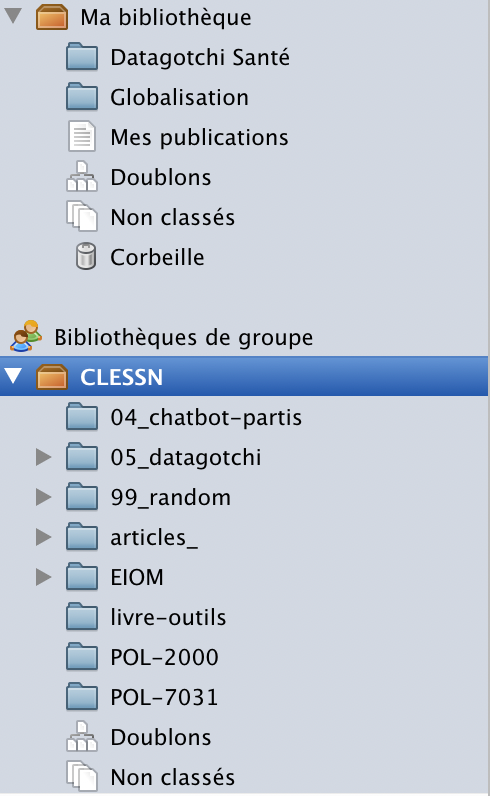
\includegraphics[width=1.77083in,height=\textheight]{images/chapitre6_zotero.png}

\emph{Il est important de comprendre que tout changement que vous faites
dans Zotero sera automatiquement synchronisé avec le groupe de votre
équipe de travail. Ainsi, si vous supprimez une référence, elle sera
supprimée pour tout le monde!}

Clic-droit sur la collection livre-outils \textgreater{} Export
Collection choisissez le format Better BibLaTex et cochez la case
{[}x{]} Keep updated. Faites OK et sauvegardez le fichier dans le
dossier .git du projet livre-outils. Ce dossier sera constamment mis à
jour avec les changements que vous faites dans Zotero et sera
synchronisé avec le projet Github quand vous ferez vos pull requests.

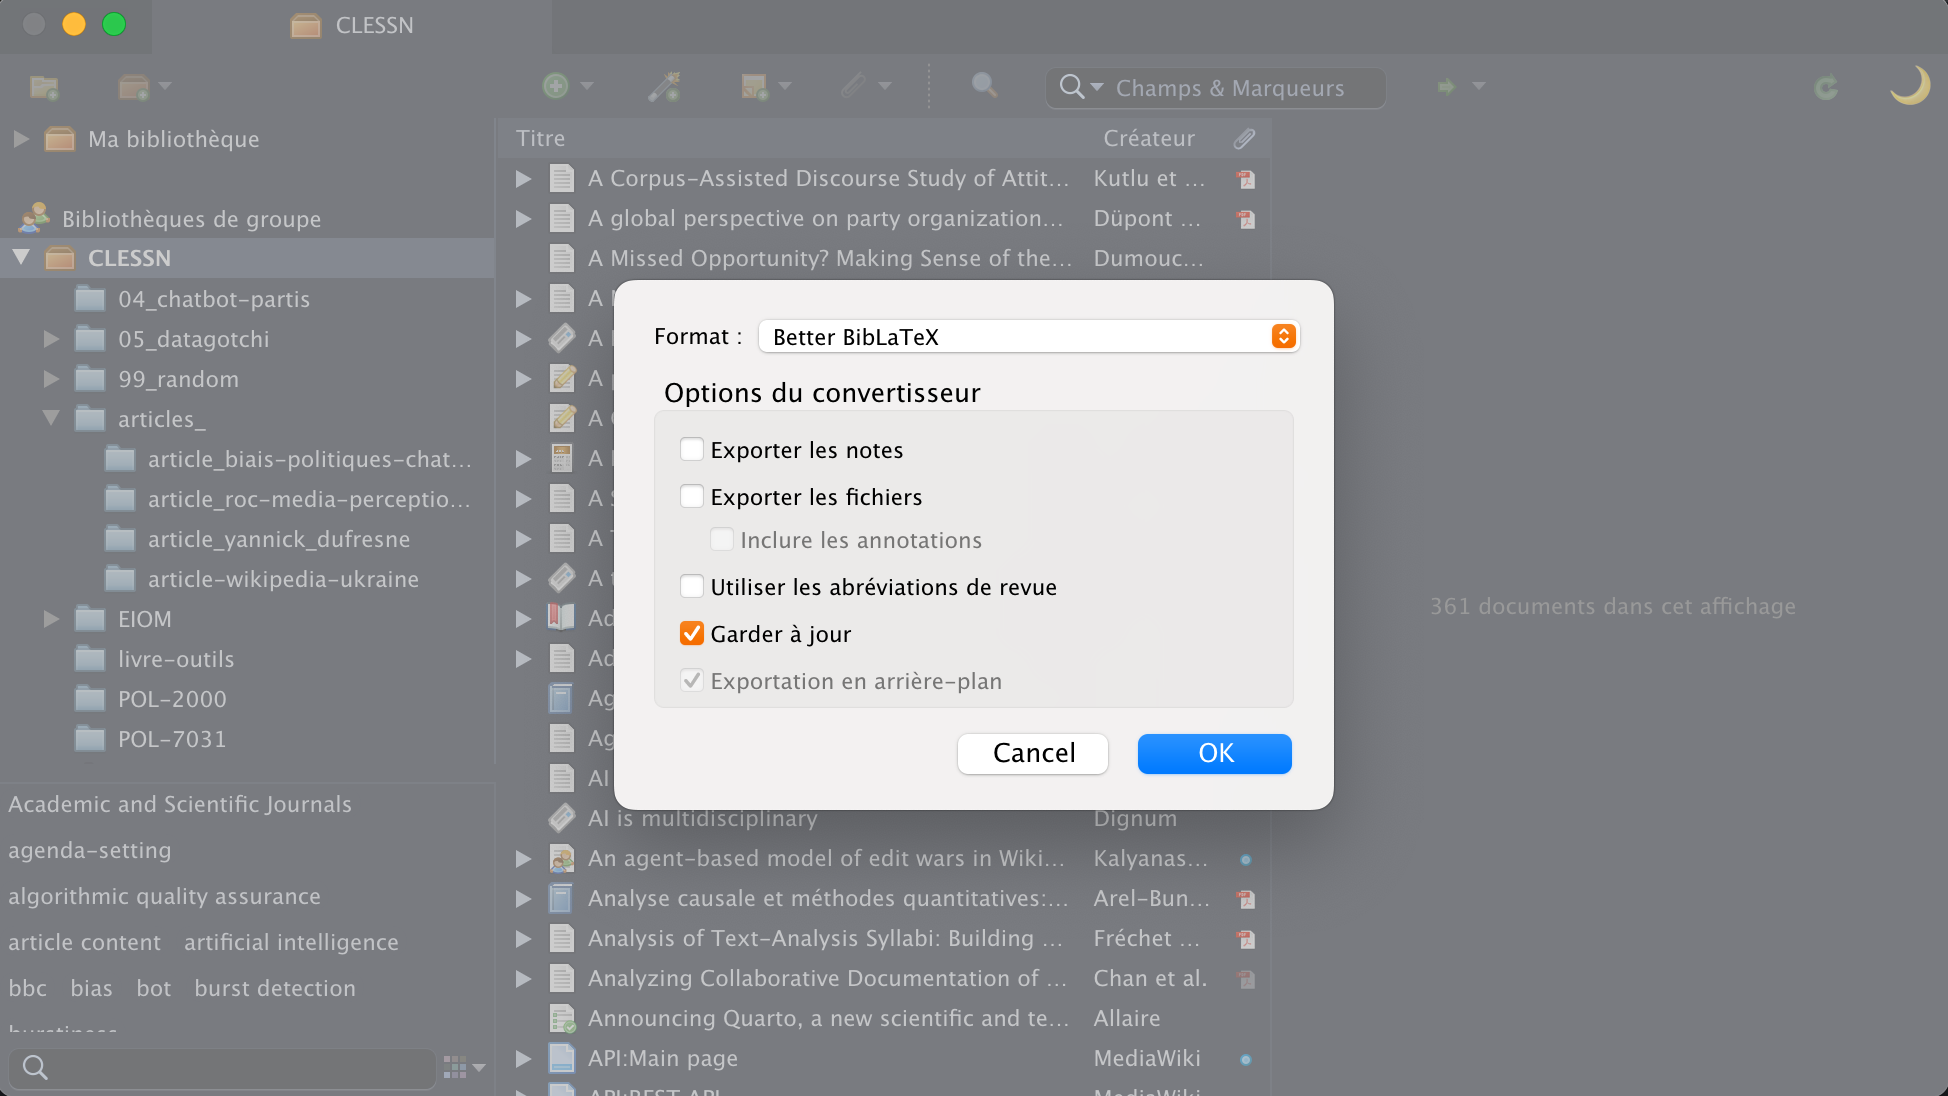
\includegraphics[width=3.125in,height=\textheight]{images/chapitre6_biblatex.png}

\subsubsection{Utilisation de Zotero lors de
l'écriture}\label{utilisation-de-zotero-lors-de-luxe9criture}

Lors de l'écriture, vous n'avez qu'a écrire @ dans votre éditeur pour
faire sortir la palette de référencement.

\subsubsection{Ajouter des références à
Zotero}\label{ajouter-des-ruxe9fuxe9rences-uxe0-zotero}

Il y a différentes façons d'ajouter des références à Zotero :

\begin{itemize}
\tightlist
\item
  Glisser-déposer à partir de votre bibliothèque personnelle.
\item
  Glisser-déposer les PDF que vous avez sur votre ordinateur dans la
  collection Livres-Outils. Zotero va essayer de trouver les métadonnées
  automatiquement.
\item
  Si cela ne réussit pas, vous pourrez ajouter la référence en cliquant
  sur la baguette magique en haut à gauche du symbole ``+'' vert.
  L'outil de la baguette magique est utile si vous possédez le DOI ou
  l'ISBN de l'article/livre que vous devez ajouter. Dans les rares cas
  où Zotero ne trouve rien concernant votre référence, vous pourrez
  remplir les différents champs manuellement.
\item
  \bookmarksetup{startatroot}

  \chapter{Utiliser le connecteur dans votre navigateur. Zotero tentera
  également de télécharger l'article directement et de l'inclure dans la
  collection
  appropriée.}\label{utiliser-le-connecteur-dans-votre-navigateur.-zotero-tentera-uxe9galement-de-tuxe9luxe9charger-larticle-directement-et-de-linclure-dans-la-collection-appropriuxe9e.}

  \begin{quote}
  \begin{quote}
  \begin{quote}
  \begin{quote}
  \begin{quote}
  \begin{quote}
  \begin{quote}
  091d1975fd7bd0b76b020ed764a52e4120eeb8a9
  \end{quote}
  \end{quote}
  \end{quote}
  \end{quote}
  \end{quote}
  \end{quote}
  \end{quote}
\end{itemize}

\bookmarksetup{startatroot}

\chapter{Outils de collecte de
données}\label{outils-de-collecte-de-donnuxe9es}

La révolution numérique engendrée par l'émergence du Big Data représente
un important défi pour le monde des sciences sociales (Manovich, 2011;
Burrows et Savage, 2014). Elle constitue également une opportunité de
recherche enrichissante et innovante permettant une compréhension plus
accrue des phénomènes sociaux étudiés par la communauté scientifique
(Connelly et al., 2016). Cette meilleure compréhension est permise,
entre autres, par l'accès à des données massives concernant les trois
acteurs clés de la société démocratique: les citoyens, les médias et les
décideurs (Schroeder, 2014; Kramer, 2014). Si l'accès à ces données
représente un défi éthique et théorique, tel qu'explicité lors des
chapitres précédents, elle représente également un défi technique pour
les chercheurs.euses voulant exploiter le potentiel et les opportunités
offertes par les données massives (Burrows et Savage, 2014).~

Le chapitre qui suit vise à offrir un portrait des outils de collectes
de données pouvant être exploitées par les scientifiques désirant
entreprendre des recherches en sciences sociales numériques. Toutefois,
la portée de ce chapitre s'étend plus loin que les outils traditionnels
de collecte de données en abordant le potentiel émanant de la
programmation en matière de collecte de données brutes pouvant être
analysées par les chercheurs.ses. Les lignes suivantes mettront un
accent particulier sur le web scraping et les opportunités de recherche
qui en découlent. Ce chapitre offre donc un tour d'horizon des outils
disponibles à la communauté scientifique tout en présentant les manières
d'exploiter le web scraping et en offrant des exemples concrets de son
utilisation.

\section{\texorpdfstring{\textbf{Point d'observation: les outils
traditionnels de collecte de données numériques en sciences
sociales}}{Point d'observation: les outils traditionnels de collecte de données numériques en sciences sociales}}\label{point-dobservation-les-outils-traditionnels-de-collecte-de-donnuxe9es-numuxe9riques-en-sciences-sociales}

Le champ d'étude de la science politique repose sur l'étude de trois
types d'acteurs distincts ayant un impact sur la condition
socio-économique et politique d'une société : les décideurs, les médias
et les citoyens. La recherche sur les décideurs comprend entre autres
l'analyse des politiques publiques, des partis politiques, de stratégies
électorales ou encore l'analyse de discours de politiciens ou
d'organisations. L'étude des médias repose largement sur le rôle des
médias dans la formation des priorités et des jugements des citoyens
quant aux enjeux politiques, de même que sur leur capacité d'influencer
l'agenda des politiciens. En ce qui concerne les citoyens, le champ
d'étude de l'opinion publique se consacre à l'analyse des comportements
et des attitudes politiques des individus. De plus, de nombreuses
recherches visant à comprendre le rôle des citoyens dans une société
démocratique portent sur l'influence de la société civile de même que
sur l'effet des mouvements sociaux.~

L'opinion publique est traditionnellement étudiée par le biais de
données de sondages. L'émergence des technologies numériques a
grandement transformé la collecte de données de sondages, qui sont
désormais conceptualisés et administrés de manière beaucoup plus
efficace. En effet, le numérique permet donc de créer un questionnaire,
de cibler une population et de la contacter, d'entreposer les données
des répondants pour ainsi les visualiser, le tout à un coût réduit et
plus rapidement que s'il avait été conduit manuellement (Nayak \& K. A.,
2019). Ainsi, les sondages en ligne ont une portée internationale,
permettent le suivi de la ligne du temps, offrent des options qui
contraignent le répondant à répondre à certaines questions et permettent
d'utiliser des arbres de logique avancés que les sondages manuels ne
permettent pas. Parmi les plateformes web les plus reconnues de
construction et d'Administration de sondage, Qualtrics figure en tête de
liste. Cette plateforme est une des plus reconnues et utilisée à
l'international, tant dans le milieu académique que dans le secteur
privé. En plus d'offrir des outils de collecte de données et de
sondages, Qualtrics est utilisé dans le marketing et dans la gestion de
l'expérience client. Il est donc pertinent de se familiariser avec cet
outil, car il offre des compétences pratiques pour la recherche, mais
également pour obtenir des opportunités de carrière. Qualtrics offre
plusieurs services pratiques pour la collecte de données, avec des
options flexibles pour la programmation et l'administration des
sondages. Par exemple, Qualtrics s'adapte à différents formats en
fonction de l'appareil du répondant (Evans \& Mathur, 2018). Son
principal désavantage provient de son coût d'acquisition, qui est
relativement dispendieux.~

Au niveau des médias, l'arrivée de données massives permet de nouvelles
avenues de recherche pour les chercheurs.euses en sciences sociales en
raison de l'importante quantité de données accessibles aux
chercheurs.euses, ce qui permet une compréhension accrue des réalités
médiatiques modernes, marquées par la fragmentation. L'outil Factiva
offre un accès à l'ensemble des articles d'une panoplie de médias
provenant d'une vaste sélection de pays. Le moteur de recherche est
opéré par Dow Jones et offre également l'accès à des documents
d'entreprises. En revanche, l'accès qu'il offre aux contenus médiatiques
est particulièrement pertinent pour la communauté scientifique en
communication et en sciences sociales. Il offre l'accès à plus de 15 000
sources médiatiques provenant de 120 pays. Il permet de télécharger une
quantité illimitée de documents RTF, un format de fichier de texte,
pouvant contenir jusqu'à 100 articles chacun. En outre, ils peuvent être
sélectionnés automatiquement en cochant le bouton proposant de
sélectionner les 100 articles de la page de résultat. Chaque page de
résultat contient 100 articles à la fois. Enfin, Factiva permet
également de filtrer les doublons. Ainsi, Factiva permet d'avoir accès
facilement à des données utiles pour l'analyse textuelle d'articles
médiatiques. Comme les textes deviennent accessibles rapidement et
simplement aux chercheurs.euses, cet outil optimise considérablement
l'analyse de contenu par thèmes ou par ton. Cependant, ce ne sont pas
tous les médias qui sont accessibles sur Factiva. Dans l'optique ou un
média recherché n'est pas trouvable sur Factiva, le logiciel Eureka
représente une bonne alternative. Eureka se concentre principalement sur
les médias francophones (autant au Québec qu'en Europe). La structure
d'Eureka est similaire à celle de Factiva.~

\section{}\label{section}

\begin{figure}[H]

{\centering 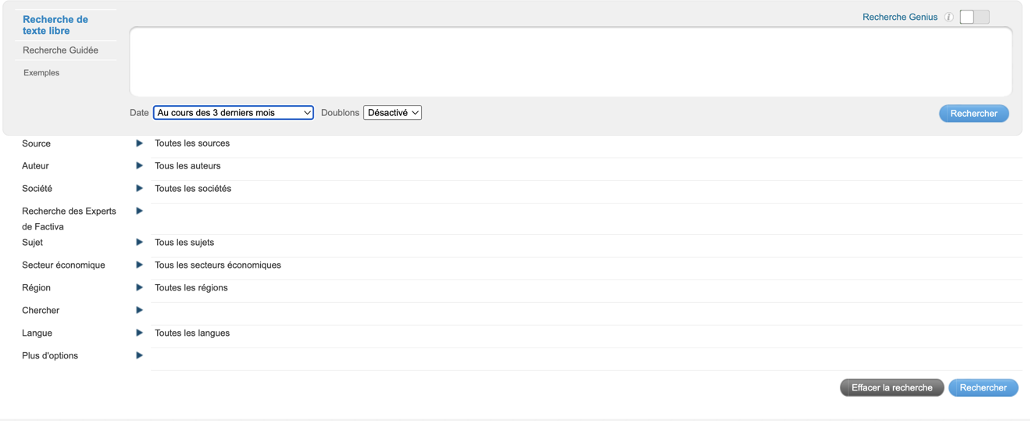
\includegraphics{images/chapitre3_factiva.png}

}

\caption{image3\_1}

\end{figure}%%
\begin{figure}[H]

{\centering 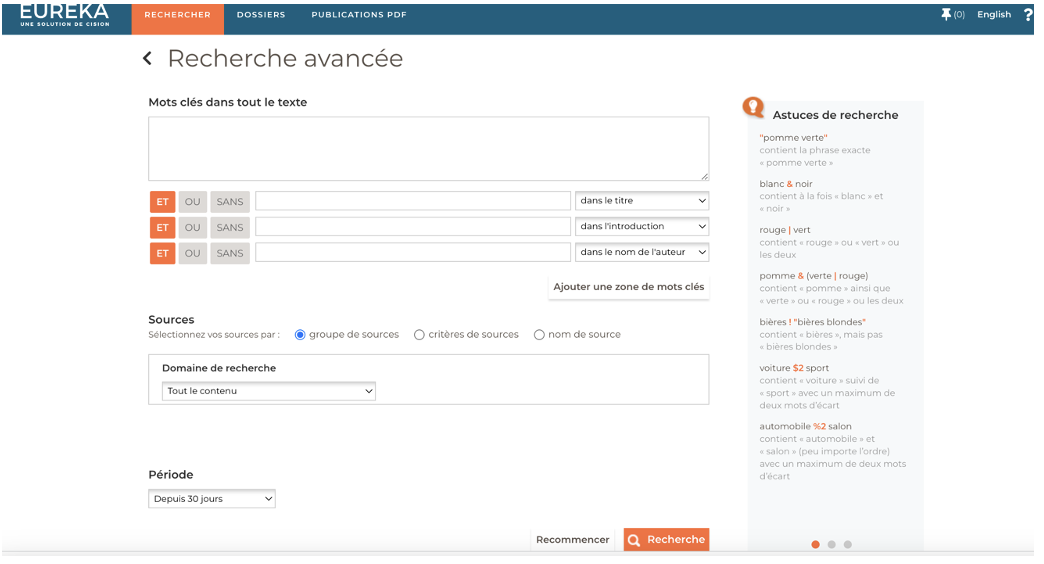
\includegraphics{images/chapitre3_eureka.png}

}

\caption{image3\_2}

\end{figure}%

\subsection{PIÈGE: NE PAS SE RESTREINDRE AUX OUTILS TRADITIONNELS DE
RECHERCHE.}\label{piuxe8ge-ne-pas-se-restreindre-aux-outils-traditionnels-de-recherche.}

Ces outils sont très utiles et relativement faciles à utiliser. Il ne
faut toutefois pas tomber dans le piège de se limiter aux outils
traditionnels de recherche. En effet, les récentes transformations
technologiques élargissent considérablement le champ de possibilités
offertes à la communauté scientifique, notamment en raison de la nature
massive des données qui lui est accessible. Non seulement ces données
sont nombreuses, mais elles sont accessibles par le biais de
connaissances de base en programmation. La section suivante aborde un
outil fondamental de la collecte de données en sciences sociales
numériques, les extracteurs webs.

\section{\texorpdfstring{\textbf{Arpentage et choix éditorial: le web
scraping - collecter automatiquement des données provenant de sites
web}}{Arpentage et choix éditorial: le web scraping - collecter automatiquement des données provenant de sites web}}\label{arpentage-et-choix-uxe9ditorial-le-web-scraping---collecter-automatiquement-des-donnuxe9es-provenant-de-sites-web}

Chacun des acteurs démocratiques énumérés précédemment peut également
être étudié par le biais d'extracteurs qui offrent un accès à des
données numériques massives. Les extracteurs de données numériques sont
des infrastructures de code permettant d'extraire des données brutes
d'une source numérique définie. La section suivante explique comment ces
extracteurs peuvent être utiles dans un contexte de recherche en
sciences sociales numériques.

L'émergence du numérique représente une opportunité hors pair d'accès à
un volume important de données, qui permettent ainsi une analyse
approfondie des phénomènes politiques contemporains. Toutefois, l'accès
à de telles données peut s'avérer complexe, non-fiable ou encore
coûteux. Par exemple, des données parlementaires peuvent être
accessibles sur les sites internet des parlements et institutions en
questions. L'accès à ces données se voit toutefois complexifié par la
nécessité d'avoir des identifiants ou encore de payer pour les dites
données. De plus, la qualité de ces données n'est pas assurée, en plus
du fait qu'elles peuvent être mal-structurées. Ainsi, l'accès à des
données massives représente un défi considérable pour la communauté
scientifique tentant d'entreprendre des recherches utilisant un volume
important de données.

C'est dans cette optique que les extracteurs de données numériques
peuvent être utiles. Plus précisément, le web scraping permet
l'extraction de données provenant de sites webs qui seront ensuite
converties dans un format utile aux scientifiques de données. Dans un
contexte de recherche en science politique, le développement de scrapers
permet de récolter automatiquement les données de sites internets
pertinents qui pourront ensuite être utilisées afin de mener à terme un
projet de recherche. Les sites desquels les données seront extraites
dépendent du sujet de recherche d'intérêt de la personne entreprenant la
recherche. Par exemple, un code peut extraire de manière automatisée les
débats des parlements, les communiqués de presse des gouvernants, les
plateformes électorales des partis politiques, ce qui offre un accès
inégalé aux chercheurs.euses aux données de décideurs. De telles données
pourraient mener à des analyses poussées sur le contenu et le ton des
débats parlementaires. Dans une autre optique, des extracteurs peuvent
également offrir l'accès aux données provenant de médias socionumériques
comme Twitter (maintenant X) ou Facebook . Un extracteur peut, par
exemple, être en mesure de répertorier l'ensemble des Tweets de
journalistes, de politiciens ou encore de citoyens de manière
automatisée, offrant un accès inégalé aux chercheurs.euses à des données
massives exclusives.

\subsection{PIÈGE: LA LÉGALITÉ DES EXTRACTEURS DE
DONNÉES}\label{piuxe8ge-la-luxe9galituxe9-des-extracteurs-de-donnuxe9es}

Il faut toutefois être vigilant quant à la nature des données extraites.
Avant d'extraire quelconque information, il est absolument primordial de
s'assurer que les données soient publiques, faute de quoi l'extraction
serait illégale. Il est donc recommandé de prendre connaissance des
termes et conditions des sites webs étudiés afin de s'assurer de la
légalité de l'extraction de données. Il est également important de
respecter toute norme de droit d'auteurs et de propriété intellectuelles
ou physique des données. De plus, ce n'est pas parce que des données
sont publiques qu'il est nécessairement légal de les extraire et de les
utiliser en recherche. En effet, il ne faut pas faire ressortir dans les
données extraites quelconque information privée qui pourrait permettre
d'identifier des individus (comme des numéros de téléphone, des adresses
courriels, des codes postaux, etc.)~

\subsection{RACCOURCI: LES API.}\label{raccourci-les-api.}

L'élaboration d'extracteurs est toutefois facilitée par l'existence
d'API (Application programming interface) sur les plateformes
exploitées. L'API d'un site ou d'une application, souvent fournie par le
site, permet à un tierce partie d'avoir accès à du code expliquant le
fonctionnement de la plateforme étudiée, ce qui en facilite l'extraction
de données. Par exemple, Twitter possédait, avant les changements de
directions récents, un API qui facilitait l'élaboration d'un extracteur.
En contrepartie, Facebook ne possède pas d'API, ce qui rend l'accès à
ses données beaucoup plus complexe. Un API fournit des données
structurées dans un format lisible tel que JSON (JavaScript Object
Notation). En raison de l'automatisation, les API réduisent les chances
d'erreurs dans le processus de scraping, ils ont tendance à maintenir
une interface plus stable et conviviale. C'est un grand changement
comparé aux fichiers HTML, où ces derniers ont des mises en page qui
changent fréquemment de structure.

Un extracteur peut également offrir l'accès à des données médiatiques,
en codant un accès à des fils RSS ou encore aux HTML des médias
extraits. Les fils RSS sont des formats de données qu'il est possible de
recevoir automatiquement lors de mise à jour sur un site particulier.
Par exemple, La Presse change ses Unes plusieurs fois dans une même
journée. En extractant l'accès aux fils RSS, il est possible de recevoir
lesdites mises à jour automatiquement. Ce processus accélère grandement
la collecte de données. Bien que les API aient souvent une limite de
taux, restreignant le nombre de requêtes possible, cela aide à éviter la
surcharge sur les serveurs et garantit en même temps une utilisation
équitable des ressources.

Finalement, les API simplifient le travail de chacun et chacune par les
mises à jour et maintenances. Pour être plus précis, les API, étant
maintenus par les fournisseurs de services, sont modifiés au fur et à
mesure que le site évolue. Par exemple, si la structure de X est
modifiée, son API sera également modifié. Cela évite à ceux demandant
l'accès d'ajuster leurs scripts de scraping pour prendre en compte les
changements sur le site.

En somme, l'utilisation d'extracteurs webs facilite grandement
l'acquisition de données massives. Plutôt que d'avoir à payer pour des
données dont la qualité n'est pas assurée, l'utilisation d'extracteurs
permet un accès plus facile et précis à des données provenant de sites
web. L'élaboration d'un extracteur est toutefois une tâche complexe qui
requiert un certain nombre de connaissances en lien avec les langages de
programmation. Le chapitre 2 du présent ouvrage offre un survol du
langage fonctionnel R, qui est utilisé par de nombreux développeurs lors
de l'écriture d'extracteurs. R est également reconnu pour ces
fonctionnalités statistiques qui sont, elles aussi, abordées
ultérieurement dans ce livre. L'utilisation d'extracteurs webs
permettent aux chercheurs.euses de faire plusieurs coups d'une seule
pierre. Non seulement le développement d'extracteurs permet de se
familiariser avec le langage R, qui est un atout essentiel dans la
recherche en sciences sociales numériques, mais ce même développement
permet un accès inégalé à des données massives qui pourront ensuite être
analysées. Le développement d'extracteurs est donc relativement simple
dépendamment du site que l'on vise à extraire. Ainsi, des connaissances
en R sont essentielles au développement d'extracteurs, et la complexité
du code évoluera dépendamment du site qui sera extrait. La section
suivante présente les outils nécessaires à l'entreprise d'extraction de
données web sur R.

\subsection{Critères de sélection}\label{crituxe8res-de-suxe9lection-1}

Le web scraping est un outil accessible, particulièrement comme il
s'agit d'une méthode libre de coûts monétaires. En effet, à moins de
circonstances exceptionnelles, le web scraping est gratuit. Le coût
serait plutôt dans l'acquisition de connaissances préalables en code
puis dans l'apprentissage de la méthode. Malgré cette nuance, l'absence
de coûts monétaires liés à cet outil favorise son accessibilité à
l'ensemble de la communauté scientifique.

Additionnellement, le web scraping jouit d'une grande communauté
d'utilisateurs.ices rendant accessible leurs connaissances, ce qui
favorise la diffusion des savoirs liés à l'utilisation de cet outil. De
nombreux forums d'aide peuvent alors être consultés gratuitement par les
chercheurs.euses voulant se familiariser avec le web scraping. De
nombreux forums sont présents sur le site Stack Overflow, et certains
chapitres d'ouvrages collectifs vulgarisant l'utilisation de l'outil
sont également dispinible gratuitement en ligne (voir par exemple le
chapitre \emph{Web scraping} du livre \emph{R for Data Science} d'Hadley
Wickham, 2022).

Le web scraping est un outil de recherche très en vogue dans la
communauté des sciences sociales. La possibilité d'obtenir une quantité
importante de données de manière efficace et gratuite représente une
opportunité depuis largement exploitée par les chercheurs.euses en
sciences sociales, en témoigne l'émergence de cours dédiés au web
scraping dans de nombreuses écoles méthodologiques de renom (telles
qu'ICPSR ou l'école d'été méthodologique du European Consortium for
Political Research).

Le web scraping avec le logiciel R permet de récolter des données qui
pourront ensuite être traitées et exploiter avec R, ce qui favorise donc
la compatibilité de l'outil. De plus, les données extraites peuvent être
exportées dans de nombreux formats tels que des fichiers .csv, .RDS,
.xlsx, et plus encore.

Tel q'explicité précédemment, la présence d'une grande communauté
d'utilisateurs.ices de l'outil favorise la transparence et la
réplicabilité des différents résultats produits lors de l'utilisation du
web scraping.

\section{Manuel d'instruction: extraire des données avec
R}\label{manuel-dinstruction-extraire-des-donnuxe9es-avec-r}

\subsection{L'importance de comprendre la structure du code
HTML}\label{limportance-de-comprendre-la-structure-du-code-html}

Afin d'être à l'aise avec les extracteurs web, il peut être un atout de
se familiariser avec la structure de base du langage HTML, dont
l'acronyme signifie ``Hypertext Markup Language''. Il s'agit d'un
langage de code qui permet la description du contenu de la page web. La
structure du code HTML est hiérarchique, ce qui signifie que le code est
divisé en différentes sections qui occupent différents rôles. Ces
sections sont délimitées par des ``tags'', qui définissent le début ou
la fin d'une section du site. Ce sont ces différentes sections qui
seront accessibles pour l'extraction, et le code HTML permet de
comprendre ce qui se situe dans ces sections. La Figure {[}{]}
représente un exemple de base de code HTML.~

\begin{figure}[H]

{\centering 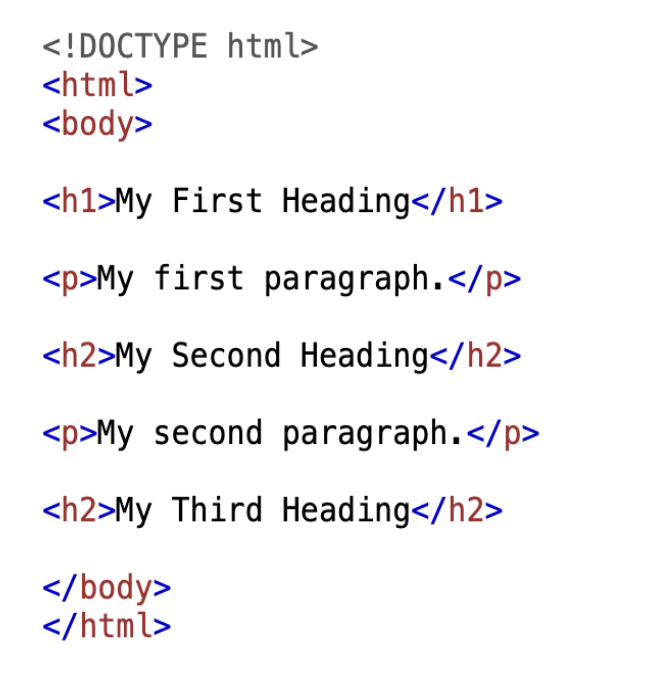
\includegraphics{images/chapitre5_html_input.png}

}

\caption{image3\_3}

\end{figure}%

Dans l'exemple ci-haut, le tag \textless h1 représente le titre du HTML.
Le signe \textless p permet de débuter le paragraphe de texte suivant le
titre, et cette section devra être terminée par le sigle p\textgreater.
Les sections \textless p\textgreater{} délimitent les paragraphes écrits
dans chacunes des sections. Les sigles \textless h2\textgreater{}
produisent une sous-section et un sous titre, qui pourra être
complémenté d'un paragraphe écrit. La Figure 2 démontre le texte produit
par le code HTML.

\begin{figure}[H]

{\centering 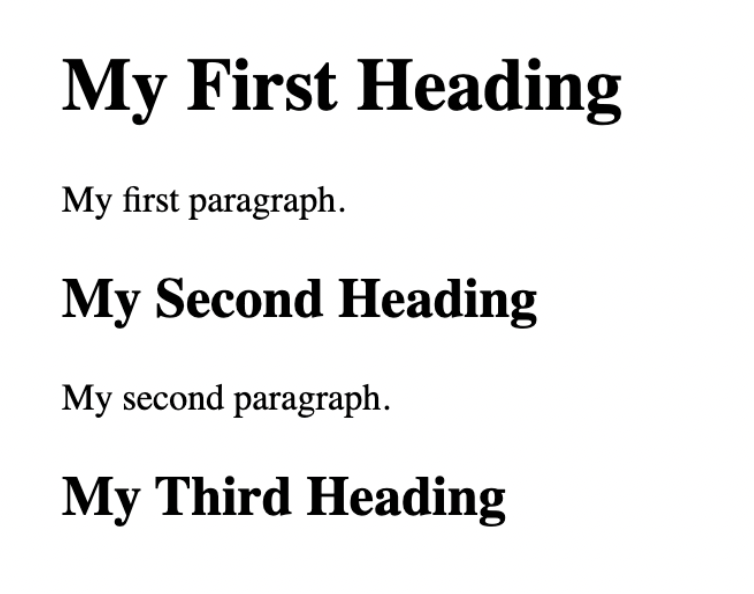
\includegraphics{images/chapitre5_html_output.png}

}

\caption{image3\_4}

\end{figure}%

La structure de base du langage HTML est somme toute simple et intuitive
et tous les sites web sur internet sont fondés sur du code HTML.
N'importe qui étant intéressé à extraire des données de sites webs et
tirer profit de la simplicité et l'accessibilité des données qui peuvent
en émerger devraient donc se familiariser avec ce langage. De nombreuses
sources en ligne sont disponibles afin d'apprendre sur le fonctionnement
du code HTML. Nous vous encourageons donc fortement à explorer plus en
profondeur les structures du code HTML afin d'obtenir une compréhension
accrue du fonctionnement des sites webs que vous allez extraire. Comme
le code HTML de chaque site est accessible grâce à l'URL, les données
présentes sur des sites webs sont plus que jamais accessible à la
communauté scientifique.

\subsection{\texorpdfstring{\textbf{Le package rvest: son fonctionnement
et ses
possibilités}}{Le package rvest: son fonctionnement et ses possibilités}}\label{le-package-rvest-son-fonctionnement-et-ses-possibilituxe9s}

Cet ouvrage recommande l'utilisation du paquetage ``Rvest'' afin de
récolter des données sur des pages web, qu'elles aient ou non un API.
Rvest est construit autour des paquetages ``xml2'' et ``httr'' afin de
faciliter la manipulation du HTML et XML. Rvest est principalement conçu
pour scraper une seule page web alors que pour scraper de multiples
pages, d'autres paquetages sont recommandés, notamment ``polite''. Cet
ouvrage ne rentre pas dans les détails et ne se concentrera que sur
Rvest.

\subsubsection{\texorpdfstring{\textbf{Fonctions de base du paquetage
rvest utilisant pour exemple le site de
LEGISinfo}}{Fonctions de base du paquetage rvest utilisant pour exemple le site de LEGISinfo}}\label{fonctions-de-base-du-paquetage-rvest-utilisant-pour-exemple-le-site-de-legisinfo}

La première étape est l'installation et le chargement des paquetages
``tidyverse'' et ``rvest'' sur sa console Rstudio. Il est important de
les charger séparément car RVEST ne fait pas partie des paquetages de
base du TIDYVERSE. Nous installerons ce dernier car il amène des
fonctions pratiques au scraping

\begin{Shaded}
\begin{Highlighting}[]
\ExtensionTok{install.packages}\ErrorTok{(}\StringTok{"rvest"}\KeywordTok{)}

\ExtensionTok{install.packages}\ErrorTok{(}\StringTok{"tidyverse"}\KeywordTok{)}

\ExtensionTok{library}\ErrorTok{(}\ExtensionTok{rvest}\KeywordTok{)}

\ExtensionTok{library}\ErrorTok{(}\ExtensionTok{tidyverse}\KeywordTok{)}
\end{Highlighting}
\end{Shaded}

Pour débuter l'extraction des données, il suffit de copier~ l'URL de la
page web à scraper et la coller dans l'appel de la fonction
read\_html(). Il est important de stocker l'URL dans l'objet
``html\_LEGISinfo.

\begin{Shaded}
\begin{Highlighting}[]
\ExtensionTok{html\_LEGISinfo} \OperatorTok{\textless{}}\NormalTok{{-} read\_html}\ErrorTok{(}\StringTok{"https://www.parl.ca/legisinfo/en/bills"}\KeywordTok{)}

\ExtensionTok{html\_LEGISinfo}
\end{Highlighting}
\end{Shaded}

Lors de l'exécution des lignes de code ci-hautes, la console retournera
les éléments suivants:

\begin{Shaded}
\begin{Highlighting}[]
\ExtensionTok{\{html\_document\}}
\OperatorTok{\textless{}}\NormalTok{html }\VariableTok{lang}\OperatorTok{=}\StringTok{"en"} \ExtensionTok{xml:lang=}\StringTok{"en"}\NormalTok{ xmlns=}\StringTok{"http://www.w3.org/1999/xhtml"}\OperatorTok{\textgreater{}}
\ExtensionTok{[1]} \OperatorTok{\textless{}}\NormalTok{head}\OperatorTok{\textgreater{}}\DataTypeTok{\textbackslash{}n}\OperatorTok{\textless{}}\NormalTok{meta http{-}equiv=}\StringTok{"Content{-}Type"}\NormalTok{ content=}\StringTok{"text/html;         charset=UTF{-}8"}\OperatorTok{\textgreater{}}\DataTypeTok{\textbackslash{}n}\OperatorTok{\textless{}}\NormalTok{meta  ...}
\ExtensionTok{[2]} \OperatorTok{\textless{}}\NormalTok{body class=}\StringTok{"body{-}wrapper ce{-}parl vh{-}100"}\OperatorTok{\textgreater{}}\DataTypeTok{\textbackslash{}r\textbackslash{}n}    \OperatorTok{\textless{}}\NormalTok{header class=}\StringTok{"d{-}print{-}none"}\OperatorTok{\textgreater{}\textless{}}\NormalTok{!{-}{-} ...}
\end{Highlighting}
\end{Shaded}

Une fois que les éléments que l'on souhaite extraire sont déterminés, il
faut les trouver dans le document HTML. Pour ce faire, il faut se
référer au style CSS (cascading style sheets), langage définissant la
forme visuelle d'un document HTML. Les éléments HTML sont identifiés
avec des ``sélecteurs CSS'', ayant pour but de les regrouper pour
faciliter leur extraction. Pour les bases du scraping, il n'est pas
primordial de comprendre les détails des sélecteurs CSS. Seule la
compréhension de la structure d'un document HTML est nécessaire afin
d'en faire l'extraction d'éléments. L'important est d'être en mesure
d'identifier les sélecteurs CSS liés aux éléments souhaités, sans avoir
à comprendre le sélecteur en question.

D'abord, html\_elements doit être utilisé en premier pour trouver toutes
les observations souhaitées, car cette fonction retourne une liste de
tous les noeuds qui matchent avec l'appel de fonction. Le nombre
d'observations est indiqué par xml\_nodeset(). Comme html\_element
retourne seulement le premier élément qui match, il faut l'utiliser en
deuxième, après html\_elements. Cette seconde fonction à pour but de
trouver les éléments qui deviendront les variables à extraire. Pour
l'exemple de LEGISinfo, nous commencerons par extraire tous les éléments
\textless a\textgreater. Comme html\_elements retourne une liste, nous
voulons commencer avec cette fonction.~

\begin{Shaded}
\begin{Highlighting}[]
\ExtensionTok{html\_LEGISinfo} \KeywordTok{|}\OperatorTok{\textgreater{}}\NormalTok{ html\_elements}\KeywordTok{(}\StringTok{"a"}\KeywordTok{)}
\end{Highlighting}
\end{Shaded}

Qui retourne les éléments suivants:

\begin{Shaded}
\begin{Highlighting}[]
\ExtensionTok{\{xml\_nodeset} \ErrorTok{(}\ExtensionTok{180}\KeywordTok{)}\ErrorTok{\}}
 \ExtensionTok{[1]} \OperatorTok{\textless{}}\NormalTok{a href=}\StringTok{"\#StartOfContent"}\NormalTok{ class=}\StringTok{"ce{-}parl{-}skipnav sr{-}only sr{-}only{-}focusable"}\OperatorTok{\textgreater{}}\NormalTok{Skip to m ...}
 \ExtensionTok{[2]} \OperatorTok{\textless{}}\NormalTok{a href=}\StringTok{"//www.parl.ca"}\NormalTok{ class=}\StringTok{"ce{-}parl{-}btn float{-}left text{-}nowrap"}\OperatorTok{\textgreater{}}\NormalTok{Parliament of Cana ...}
 \ExtensionTok{[3]} \OperatorTok{\textless{}}\NormalTok{a href=}\StringTok{"https://visit.parl.ca/index{-}e.html"}\NormalTok{ rel=}\StringTok{"external"}\OperatorTok{\textgreater{}}\DataTypeTok{\textbackslash{}n\textbackslash{}t\textbackslash{}t}\NormalTok{                    ...}
\end{Highlighting}
\end{Shaded}

\begin{Shaded}
\begin{Highlighting}[]
\ExtensionTok{html\_LEGISinfo} \KeywordTok{|}\OperatorTok{\textgreater{}}\NormalTok{ html\_elements}\KeywordTok{(}\StringTok{"a"}\KeywordTok{)}
\end{Highlighting}
\end{Shaded}

Qui retourne les éléments suivants:

\begin{Shaded}
\begin{Highlighting}[]
\ExtensionTok{\{xml\_nodeset} \ErrorTok{(}\ExtensionTok{180}\KeywordTok{)}\ErrorTok{\}}
 \ExtensionTok{[1]} \OperatorTok{\textless{}}\NormalTok{a href=}\StringTok{"\#StartOfContent"}\NormalTok{ class=}\StringTok{"ce{-}parl{-}skipnav sr{-}only sr{-}only{-}focusable"}\OperatorTok{\textgreater{}}\NormalTok{Skip to m ...}
 \ExtensionTok{[2]} \OperatorTok{\textless{}}\NormalTok{a href=}\StringTok{"//www.parl.ca"}\NormalTok{ class=}\StringTok{"ce{-}parl{-}btn float{-}left text{-}nowrap"}\OperatorTok{\textgreater{}}\NormalTok{Parliament of Cana ...}
 \ExtensionTok{[3]} \OperatorTok{\textless{}}\NormalTok{a href=}\StringTok{"https://visit.parl.ca/index{-}e.html"}\NormalTok{ rel=}\StringTok{"external"}\OperatorTok{\textgreater{}}\DataTypeTok{\textbackslash{}n\textbackslash{}t\textbackslash{}t}\NormalTok{                    ...}
\end{Highlighting}
\end{Shaded}

\begin{Shaded}
\begin{Highlighting}[]
\ExtensionTok{html\_LEGISinfo} \KeywordTok{|}\OperatorTok{\textgreater{}}\NormalTok{ html\_elements}\KeywordTok{(}\StringTok{"a"}\KeywordTok{)}
\end{Highlighting}
\end{Shaded}

\begin{Shaded}
\begin{Highlighting}[]
\ExtensionTok{\{html\_node\}}
\OperatorTok{\textless{}}\NormalTok{a }\VariableTok{href}\OperatorTok{=}\StringTok{"\#StartOfContent"} \VariableTok{class}\OperatorTok{=}\StringTok{"ce{-}parl{-}skipnav sr{-}only sr{-}only{-}focusable"}\OperatorTok{\textgreater{}}
\end{Highlighting}
\end{Shaded}

Suite à l'inspection des éléments , ceux qui nous intéressent sont ceux
de classe ``bill-tile-container''. Il suffit d'ajouter un point ``.''
avant la classe souhaitée lors de l'appel de la fonction afin de
rechercher les éléments en fonction de leur classe. Les classes HTML
servent à catégoriser les éléments HTML selon un style prédéterminé.
Pour l'exemple de LEGISinfo, nous obtenons une liste d'éléments de
classe bill-tile-container que nous allons stocker dans l'objet
BillTile\_LEGISinfo. Tous les éléments de cette classe auront donc tous
une structure ou des comportements similaires entre eux.

\begin{Shaded}
\begin{Highlighting}[]
\ExtensionTok{BillTile\_LEGISinfo} \OperatorTok{\textless{}}\NormalTok{{-} html\_LEGISinfo }\KeywordTok{|}\OperatorTok{\textgreater{}}\NormalTok{ html\_elements}\KeywordTok{(}\StringTok{".bill{-}tile{-}container"}\KeywordTok{)}
\end{Highlighting}
\end{Shaded}

L'exécution du bloc de code ci-haut produit le résultat suivant dans la
console

\begin{Shaded}
\begin{Highlighting}[]
\ExtensionTok{\{xml\_nodeset} \ErrorTok{(}\ExtensionTok{60}\KeywordTok{)}\ErrorTok{\}}
 \ExtensionTok{[1]} \OperatorTok{\textless{}}\NormalTok{a class=}\StringTok{"bill{-}tile{-}container senate"}\NormalTok{ href=}\StringTok{"/legisinfo/en/bill/44{-}1/s{-}1"}\OperatorTok{\textgreater{}}\DataTypeTok{\textbackslash{}r\textbackslash{}n\textbackslash{}r\textbackslash{}n}\NormalTok{     ...}
 \ExtensionTok{[2]} \OperatorTok{\textless{}}\NormalTok{a class=}\StringTok{"bill{-}tile{-}container senate"}\NormalTok{ href=}\StringTok{"/legisinfo/en/bill/44{-}1/s{-}2"}\OperatorTok{\textgreater{}}\DataTypeTok{\textbackslash{}r\textbackslash{}n\textbackslash{}r\textbackslash{}n}\NormalTok{     ...}
 \ExtensionTok{[3]} \OperatorTok{\textless{}}\NormalTok{a class=}\StringTok{"bill{-}tile{-}container senate"}\NormalTok{ href=}\StringTok{"/legisinfo/en/bill/44{-}1/s{-}3"}\OperatorTok{\textgreater{}}\DataTypeTok{\textbackslash{}r\textbackslash{}n\textbackslash{}r\textbackslash{}n}\NormalTok{     ...}
\end{Highlighting}
\end{Shaded}

À partir de la liste d'éléments de classe bill-tile-container, nous
appelons la fonction html\_element, qui lorsque appliqué à une liste
permet d'extraire la première correspondance de tous les éléments de
cette liste au lieu de seulement retourner le premier nœud correspondant
du document HTML. Nous cherchons à extraire ici les éléments de classe
parliament-session par le biais de la ligne de code suivante:

\begin{Shaded}
\begin{Highlighting}[]
\ExtensionTok{BillTile\_LEGISinfo} \KeywordTok{|}\OperatorTok{\textgreater{}}\NormalTok{ html\_element}\KeywordTok{(}\StringTok{".parliament{-}session"}\KeywordTok{)} 
\end{Highlighting}
\end{Shaded}

Ce qui produit le résultat suivant dans la console:

\begin{Shaded}
\begin{Highlighting}[]
\ExtensionTok{\{xml\_nodeset} \ErrorTok{(}\ExtensionTok{60}\KeywordTok{)}\ErrorTok{\}}
 \ExtensionTok{[1]} \OperatorTok{\textless{}}\NormalTok{div class=}\StringTok{"parliament{-}session"}\OperatorTok{\textgreater{}}\DataTypeTok{\textbackslash{}n}\OperatorTok{\textless{}}\NormalTok{span class=}\StringTok{"parl{-}session{-}number"}\OperatorTok{\textgreater{}}\NormalTok{44th}\OperatorTok{\textless{}}\NormalTok{/span}\OperatorTok{\textgreater{}}\NormalTok{ Parlia ...}
 \ExtensionTok{[2]} \OperatorTok{\textless{}}\NormalTok{div class=}\StringTok{"parliament{-}session"}\OperatorTok{\textgreater{}}\DataTypeTok{\textbackslash{}n}\OperatorTok{\textless{}}\NormalTok{span class=}\StringTok{"parl{-}session{-}number"}\OperatorTok{\textgreater{}}\NormalTok{44th}\OperatorTok{\textless{}}\NormalTok{/span}\OperatorTok{\textgreater{}}\NormalTok{ Parlia ...}
 \ExtensionTok{[3]} \OperatorTok{\textless{}}\NormalTok{div class=}\StringTok{"parliament{-}session"}\OperatorTok{\textgreater{}}\DataTypeTok{\textbackslash{}n}\OperatorTok{\textless{}}\NormalTok{span class=}\StringTok{"parl{-}session{-}number"}\OperatorTok{\textgreater{}}\NormalTok{44th}\OperatorTok{\textless{}}\NormalTok{/span}\OperatorTok{\textgreater{}}\NormalTok{ Parlia ...}
\end{Highlighting}
\end{Shaded}

Bien que moins utile pour la mise en situation actuelle, il est
également possible d'extraire les éléments en fonction de leur ``id
attribute''. Pour ce faire, il faut mettre un hashtag (\#) avant
l'élément à extraire lors de l'appel de la fonction. Le id attribute
retourne toujours un seul élément car ils sont uniques à chaque document
HTML. Voici la ligne de code et le résultat produit par une telle
opération

\begin{Shaded}
\begin{Highlighting}[]
\ExtensionTok{html\_LEGISinfo} \KeywordTok{|}\OperatorTok{\textgreater{}}\NormalTok{ html\_elements}\KeywordTok{(}\StringTok{"\#StartOfContent"}\KeywordTok{)}
\end{Highlighting}
\end{Shaded}

\begin{Shaded}
\begin{Highlighting}[]
\ExtensionTok{\{xml\_nodeset} \ErrorTok{(}\ExtensionTok{1}\KeywordTok{)}\ErrorTok{\}}
\ExtensionTok{[1]} \OperatorTok{\textless{}}\NormalTok{a id=}\StringTok{"StartOfContent"}\NormalTok{ tabindex=}\StringTok{"{-}1"}\OperatorTok{\textgreater{}\textless{}}\NormalTok{/a}\OperatorTok{\textgreater{}}
\end{Highlighting}
\end{Shaded}

Nous avons créé précédemment l'objet BillTile\_LEGISinfo pour ensuite y
extraire les éléments de classe parliament-session. Nous appelons cette
étape l'imbrication des sélections. Lorsque la fonction html\_element
est appliquée à un vecteur de liste html\_elements, la console retourne
le premier nœud correspondant de chaque élément de la liste. Il est
important d'utiliser html\_element à cette étape car il retourne un NA
même lorsqu'il n'y a pas d'éléments correspondants, alors que
html\_elements ne retournera pas la valeur manquante. Dans l'exemple de
LEGISinfo, c'est exactement ce que l'on a voulu faire pour obtenir les
éléments de classe parliament-session. Nous sommes maintenant arrivés à
l'étape d'extraire les données souhaitées. C'est assez simple, il ne
suffit que d'appliquer la fonction html\_text2 sur l'appel de
html\_element sur l'objet à moissonner, dans ce cas ci
BillTile\_LEGISinfo. Il est important de prendre en compte que nous
connaissons ici les éléments à extraire, car le script du document a été
scruté préalablement grâce à la fonction ``inspect'' de Google Chrome
ainsi que les diverses fonctions du package rvest. Afin d'extraire les
autres informations souhaitées, nous allons également créer deux autres
objets qui seront à leur tour moissonnés. Voici les différentes
opérations et leurs résultats dans la console:

Code

\begin{Shaded}
\begin{Highlighting}[]
\ExtensionTok{BillTile\_LEGISinfo} \KeywordTok{|}\OperatorTok{\textgreater{}}\NormalTok{ html\_element}\KeywordTok{(}\StringTok{"h4"}\KeywordTok{)} \KeywordTok{|}\OperatorTok{\textgreater{}}\NormalTok{ html\_text2}\KeywordTok{()}
\end{Highlighting}
\end{Shaded}

Console

\begin{Shaded}
\begin{Highlighting}[]
\ExtensionTok{[1]} \StringTok{"S{-}1"}   \StringTok{"S{-}2"}   \StringTok{"S{-}3"}   \StringTok{"S{-}4"}   \StringTok{"S{-}5"}\NormalTok{...}
\end{Highlighting}
\end{Shaded}

Code

\begin{Shaded}
\begin{Highlighting}[]
\ExtensionTok{BillTile\_LEGISinfo} \KeywordTok{|}\OperatorTok{\textgreater{}}\NormalTok{ html\_element}\KeywordTok{(}\StringTok{".parliament{-}session"}\KeywordTok{)} \KeywordTok{|}\OperatorTok{\textgreater{}}\NormalTok{ html\_text2}\KeywordTok{()}\BuiltInTok{.}
\end{Highlighting}
\end{Shaded}

Console

\begin{Shaded}
\begin{Highlighting}[]
\ExtensionTok{[1]} \StringTok{"44th Parliament, 1st session"} \StringTok{"44th Parliament, 1st session"}\NormalTok{...}
\end{Highlighting}
\end{Shaded}

Code

\begin{Shaded}
\begin{Highlighting}[]
\ExtensionTok{BillTile\_LEGISinfo} \KeywordTok{|}\OperatorTok{\textgreater{}}\NormalTok{ html\_element}\KeywordTok{(}\StringTok{"h5"}\KeywordTok{)} \KeywordTok{|}\OperatorTok{\textgreater{}}\NormalTok{ html\_text2}\KeywordTok{()}
\end{Highlighting}
\end{Shaded}

Console

\begin{Shaded}
\begin{Highlighting}[]
\ExtensionTok{[1]} \StringTok{"An Act relating to railways"}                                                                                                                                                                                                                                                                                  
 \ExtensionTok{[2]} \StringTok{"An Act to amend the Parliament of Canada Act and to make consequential and related amendments to other Acts"}                                                                                                                                                                                                  
 \ExtensionTok{[3]} \StringTok{"An Act to amend the Judges Act"}   
\ExtensionTok{...}
\end{Highlighting}
\end{Shaded}

Code

\begin{Shaded}
\begin{Highlighting}[]
\ExtensionTok{BillBS\_LEGISinfo} \OperatorTok{\textless{}}\NormalTok{{-} html\_LEGISinfo }\KeywordTok{|}\OperatorTok{\textgreater{}}\NormalTok{ html\_elements}\KeywordTok{(}\StringTok{".bottom{-}section"}\KeywordTok{)}
\ExtensionTok{BillBS\_LEGISinfo} \KeywordTok{|}\OperatorTok{\textgreater{}}\NormalTok{ html\_element}\KeywordTok{(}\StringTok{"dd"}\KeywordTok{)} \KeywordTok{|}\OperatorTok{\textgreater{}}\NormalTok{ html\_text2}\KeywordTok{()}
\end{Highlighting}
\end{Shaded}

Console

\begin{Shaded}
\begin{Highlighting}[]
\ExtensionTok{[1]} \StringTok{"Introduced as pro forma bill"}                                              \StringTok{"Senate bill awaiting first reading in the House of Commons"}               
 \ExtensionTok{[3]} \StringTok{"Bill not proceeded with"}                                                   \StringTok{"Royal assent received"}                                                    
 \ExtensionTok{[5]} \StringTok{"Royal assent received"}                                                     \StringTok{"At second reading in the House of Commons"}     
\ExtensionTok{...}
\end{Highlighting}
\end{Shaded}

Code

\begin{Shaded}
\begin{Highlighting}[]
\ExtensionTok{Bill\_stage} \OperatorTok{\textless{}}\NormalTok{{-} html\_LEGISinfo }\KeywordTok{|}\OperatorTok{\textgreater{}}\NormalTok{ html\_elements}\KeywordTok{(}\StringTok{".progress{-}bar{-}description"}\KeywordTok{)}
\ExtensionTok{Bill\_stage} \KeywordTok{|}\OperatorTok{\textgreater{}}\NormalTok{ html\_element}\KeywordTok{(}\StringTok{"dd"}\KeywordTok{)} \KeywordTok{|}\OperatorTok{\textgreater{}}\NormalTok{ html\_text2}\KeywordTok{()}
\end{Highlighting}
\end{Shaded}

Console

\begin{Shaded}
\begin{Highlighting}[]
\ExtensionTok{[1]} \StringTok{"First reading in the Senate"}            \StringTok{"Third reading in the Senate"}            \StringTok{"First reading in the Senate"}            \StringTok{"Royal assent"}                           \StringTok{"Royal assent"}                          
 \ExtensionTok{[6]} \StringTok{"First reading in the House of Commons"}  \StringTok{"First reading in the House of Commons"}  \StringTok{"Royal assent"}                           \StringTok{"First reading in the House of Commons"}  \StringTok{"Royal assent"}        
\ExtensionTok{...}
 
\end{Highlighting}
\end{Shaded}

Maintenant que nous avons tous les éléments souhaités, il ne reste plus
qu'à utiliser la fonction tibble du tidyverse. Ce paquetage permet de
facilement créer des dataframes sur R. Voici le script à produire dans
l'exemple de LEGISinfo, ainsi que son résultat, un dataframe contenant
le numéro de projet de loi, sa session parlementaire, son nom, son
statut et son dernier stage de réalisation :

\begin{Shaded}
\begin{Highlighting}[]
\ExtensionTok{Table\_LEGISinfo} \OperatorTok{\textless{}}\NormalTok{{-} tibble}\ErrorTok{(}
  \ExtensionTok{Bill}\NormalTok{ = Bill\_LEGISinfo }\KeywordTok{|}\OperatorTok{\textgreater{}}\NormalTok{ html\_element}\KeywordTok{(}\StringTok{"h4"}\KeywordTok{)} \KeywordTok{|}\OperatorTok{\textgreater{}}\NormalTok{ html\_text2}\KeywordTok{()}\ExtensionTok{,}
  \ExtensionTok{Session}\NormalTok{ = Bill\_LEGISinfo }\KeywordTok{|}\OperatorTok{\textgreater{}}\NormalTok{ html\_element}\KeywordTok{(}\StringTok{".parliament{-}session"}\KeywordTok{)} \KeywordTok{|}\OperatorTok{\textgreater{}}\NormalTok{ html\_text2}\KeywordTok{()}\ExtensionTok{,}
  \ExtensionTok{Name}\NormalTok{ = Bill\_LEGISinfo }\KeywordTok{|}\OperatorTok{\textgreater{}}\NormalTok{ html\_element}\KeywordTok{(}\StringTok{"h5"}\KeywordTok{)} \KeywordTok{|}\OperatorTok{\textgreater{}}\NormalTok{ html\_text2}\KeywordTok{()}\ExtensionTok{,}
  \ExtensionTok{Status}\NormalTok{ = BillBS\_LEGISinfo }\KeywordTok{|}\OperatorTok{\textgreater{}}\NormalTok{ html\_element}\KeywordTok{(}\StringTok{"dd"}\KeywordTok{)} \KeywordTok{|}\OperatorTok{\textgreater{}}\NormalTok{ html\_text2}\KeywordTok{()}\ExtensionTok{,}
  \ExtensionTok{Stage}\NormalTok{ = Bill\_stage }\KeywordTok{|}\OperatorTok{\textgreater{}}\NormalTok{ html\_element}\KeywordTok{(}\StringTok{"dd"}\KeywordTok{)} \KeywordTok{|}\OperatorTok{\textgreater{}}\NormalTok{ html\_text2}\KeywordTok{()}
\KeywordTok{)}
\end{Highlighting}
\end{Shaded}

Il est important de noter que ce chapitre ne permet que de scraper des
documents html uniques. Afin de scraper plusieurs page web
simultanément, il faudra utiliser d'autres paquetages ainsi que des
boucles, ce qui est trop complexe pour cet ouvrage d'introduction.
Maintenant que vous savez extraire des informations d'un document html
pour le mettre dans une base de données, voici d'autres applications
pratiques de rvest à cet effet.

Il est possible d'extraire les éléments en fonction de leur attribut
grâce à html\_attr(). Un attribut est une information supplémentaire
associé à une balise html. Voici l'attribut href qui permet d'extraire
l'URL du projet de loi en question. De cette façon, il est possible de
boucler sur les href afin de moissonner divers niveaux d'une page HTML.
Lorsque l'extraction se fait sur plusieurs niveaux, la pratique passe du
moissonnage pour devenir de l'indexation. Cette pratique, bien que
fondamentale, ne sera pas abordée en raison de sa complexité avancée.
Tel que mentionné plus haut, cet ouvrage ne se concentre que sur le
moissonnage.

\begin{Shaded}
\begin{Highlighting}[]
\ExtensionTok{BillTile\_LEGISinfo} \KeywordTok{|}\OperatorTok{\textgreater{}}\NormalTok{ html\_attr}\KeywordTok{(}\StringTok{"href"}\KeywordTok{)}
\end{Highlighting}
\end{Shaded}

La ligne de code ci-haut produit le résultat suivant dans la console

\begin{Shaded}
\begin{Highlighting}[]
\ExtensionTok{1]} \StringTok{"/legisinfo/en/bill/44{-}1/s{-}1"}   \StringTok{"/legisinfo/en/bill/44{-}1/s{-}2"}   \StringTok{"/legisinfo/en/bill/44{-}1/s{-}3"}   \StringTok{"/legisinfo/en/bill/44{-}1/s{-}4"}   \StringTok{"/legisinfo/en/bill/44{-}1/s{-}5"}   \StringTok{"/legisinfo/en/bill/44{-}1/s{-}6"}  
 \ExtensionTok{[7]} \StringTok{"/legisinfo/en/bill/44{-}1/s{-}7"}   \StringTok{"/legisinfo/en/bill/44{-}1/s{-}8"}   \StringTok{"/legisinfo/en/bill/44{-}1/s{-}9"}   \StringTok{"/legisinfo/en/bill/44{-}1/s{-}10"}  \StringTok{"/legisinfo/en/bill/44{-}1/s{-}11"}  \StringTok{"/legisinfo/en/bill/44{-}1/s{-}12"} 
\ExtensionTok{[13]} \StringTok{"/legisinfo/en/bill/44{-}1/s{-}13"}  \StringTok{"/legisinfo/en/bill/44{-}1/s{-}14"}  \StringTok{"/legisinfo/en/bill/44{-}1/s{-}15"}  \StringTok{"/legisinfo/en/bill/44{-}1/s{-}16"}  \StringTok{"/legisinfo/en/bill/44{-}1/s{-}17"}  \StringTok{"/legisinfo/en/bill/44{-}1/s{-}201"}
\end{Highlighting}
\end{Shaded}

Il est également possible d'extraire des tables. Pour cet exemple, le
site de LEGISinfo ne comporte malheureusement pas de tables, le script
de https://r4ds.hadley.nz/webscraping sera donc utilisé. Celui-ci
utilise la fonction minimal\_html pour créer un script html, qui n'est
pas nécessaire au moissonnage, mais toutefois utilisé pour cet exemple.

\begin{Shaded}
\begin{Highlighting}[]
\ExtensionTok{htmltest} \OperatorTok{\textless{}}\NormalTok{{-} minimal\_html}\ErrorTok{(}\StringTok{"}
\StringTok{  \textless{}table class=\textquotesingle{}mytable\textquotesingle{}\textgreater{}}
\StringTok{\textless{}tr\textgreater{}\textless{}th\textgreater{}x\textless{}/th\textgreater{}   \textless{}th\textgreater{}y\textless{}/th\textgreater{}\textless{}/tr\textgreater{}}
\StringTok{\textless{}tr\textgreater{}\textless{}td\textgreater{}1.5\textless{}/td\textgreater{} \textless{}td\textgreater{}2.7\textless{}/td\textgreater{}\textless{}/tr\textgreater{}}
\StringTok{\textless{}tr\textgreater{}\textless{}td\textgreater{}4.9\textless{}/td\textgreater{} \textless{}td\textgreater{}1.3\textless{}/td\textgreater{}\textless{}/tr\textgreater{}}
\StringTok{\textless{}tr\textgreater{}\textless{}td\textgreater{}7.2\textless{}/td\textgreater{} \textless{}td\textgreater{}8.1\textless{}/td\textgreater{}\textless{}/tr\textgreater{}}
\StringTok{\textless{}/table\textgreater{}}
\StringTok{  "}\KeywordTok{)}
  \ExtensionTok{htmltest} \KeywordTok{|}\OperatorTok{\textgreater{}}
  \ExtensionTok{html\_element}\ErrorTok{(}\StringTok{".mytable"}\KeywordTok{)} \KeywordTok{|}\OperatorTok{\textgreater{}}\NormalTok{ html\_table}\KeywordTok{()}
\end{Highlighting}
\end{Shaded}

L'opération précédante produit le résultat suivant dans la console

\begin{Shaded}
\begin{Highlighting}[]
\CommentTok{\# A tibble: 3 × 2}
      \ExtensionTok{x}\NormalTok{     y}
  \OperatorTok{\textless{}}\NormalTok{dbl}\OperatorTok{\textgreater{}} \OperatorTok{\textless{}}\NormalTok{dbl}\OperatorTok{\textgreater{}}
\ExtensionTok{1}\NormalTok{   1.5   2.7}
\ExtensionTok{2}\NormalTok{   4.9   1.3}
\ExtensionTok{3}\NormalTok{   7.2   8.1}
\end{Highlighting}
\end{Shaded}

En conclusion de cette section, lorsque l'on moissonne un document HTML,
il est important de ne pas se laisser intimider par la structure du
document. Il ne faut pas perdre patience afin de trouver les bons
sélecteurs. Ce sont des structures peu familières au début, mais on s'y
habitue rapidement. Ensuite, nous recommandons d'utiliser l'outil de
développeur de votre navigateur web afin de pouvoir trouver les
sélecteurs souhaités. L'interface de Chrome est particulièrement
conviviale, et est recommandée. Il suffit de cliquer sur ``inspect''
suite à un clic droit, et il est possible de chercher les éléments
souhaités dans le script. Finalement, avant de scrapper le contenu d'un
site web, il est important de vérifier s'il n'offre pas déjà une option
pour télécharger les données ! C'est le cas de l'exemple utilisé ici
(LEGISinfo), il est possible dans certains cas de télécharger les
données directement sur le site web, ce qui rend parfois le besoin de
moissonner désuet.

\hfill\break

\section{Conclusion et discussion:}\label{conclusion-et-discussion}

Ce chapitre a comme objectif de dresser un portrait des différents
outils de collecte de données mis à la disposition des scientifiques
s'intéressant aux sciences sociales tout en voulant exploiter le
potentiel de la révolution numérique. Bien que non exhaustif, ce
chapitre fait un survol d'outils traditionnels de récolte de données
numériques en sciences sociales. Par exemple, les outils de sondages ou
de récolte de données médiatiques sont présentés dans les paragraphes
ci-haut. En revanche, ce chapitre s'ancre autour du postulat qu'il ne
faut pas se limiter aux outils de récolte de données traditionnels, et
que la révolution numérique engendre d'importantes opportunités
d'acquisition de données massives et exclusives par le biais des
extracteurs de données. Ces extracteurs ont pour but de moissonner les
données présentes sur un site web afin de les rendre disponibles pour
l'analyse scientifique. Une section complète de ce chapitre vise à
vulgariser le processus d'extraction de données provenant de site web en
utilisant l'exemple du site LégisInfo, ce qui permet aux lecteurs.ices
de se familiariser avec le processus de moissonnage de données.

Toutefois, un seul chapitre ne permet pas de relever l'ensemble des
outils de collecte de données disponibles pour la communauté
scientifique. Néanmoins, les outils présentés permettent un aperçu à la
fois d'outils plus conventionnels et répandus de collecte de données
numériques, mais également de dresser un portrait du potentiel
d'extraction permis par la maîtrise de R.

Bibliographie:

Schroeder, R. (2014). Big data and the brave new world of social media
research.~\emph{Big Data \& Society},~\emph{1}(2), 2053951714563194.

Chadwick, A. (2017). The hybrid media system: Politics and power. Oxford
University Press.

Connelly, R., Playford, C. J., Gayle, V., \& Dibben, C. (2016). The role
of administrative data in the big data revolution in social science
research.~\emph{Social science research},~\emph{59}, 1-12.

Manovich, L. (2011). Trending: The promises and the challenges of big
social data.~\emph{Debates in the digital humanities},~\emph{2}(1),
460-475.

Burrows, R., \& Savage, M. (2014). After the crisis? Big Data and the
methodological challenges of empirical sociology.~\emph{Big data \&
society},~\emph{1}(1), 2053951714540280.

Kramer, A. D., Guillory, J. E., \& Hancock, J. T. (2014). Experimental
evidence of massive-scale emotional contagion through social
networks.~\emph{Proceedings of the National academy of Sciences of the
United States of America},~\emph{111}(24), 8788.

Andrade, C. (2020). The Limitations of Online Surveys. Indian Journal of
Psychological Medicine, 42(6), 575-576.
https://doi.org/10.1177/0253717620957496

\hfill\break
Evans, J. R., \& Mathur, A. (2018). The value of online surveys: A look
back and a look ahead. Internet Research, 28(4), 854-887.
https://doi.org/10.1108/IntR-03-2018-0089

\hfill\break
Nayak, M., \& K A, N. (2019). Strengths and Weakness of Online Surveys.
24, 31-38. https://doi.org/10.9790/0837-2405053138

\bookmarksetup{startatroot}

\chapter{Outils de visualisation
graphique}\label{outils-de-visualisation-graphique}

\section{Une image vaut mille mots}\label{une-image-vaut-mille-mots}

Camille Tremblay-Antoine\footnote{Université Laval} Nadjim
Fréchet\footnote{Université de Montréal}

\section{Introduction}\label{introduction-1}

Une fois les données collectées, nettoyées, traitées et analysées, une
partie centrale du travail d'un scientifique de données est de faire
parler les résultats de ses tests empiriques. Il s'agit alors de trouver
la meilleure manière de rendre l'information digeste pour les experts et
initiés de votre discipline académique ou pour le grand public. La
visualisation graphique des données est donc centrale afin de vulgariser
les résultats d'une recherche empirique.

Mais qu'est-ce qu'une bonne visualisation de données? Quel type de
graphique choisir? Quelles couleurs utiliser? Quelles informations
mettre en évidence? Ce chapitre ne répond pas à ces questions, une
myriade d'ouvrages les ont déjà traitées. Du classique \emph{The Visual
Display of Quantitative Information} de Edward Tufte (1983) jusqu'aux
plus récents ouvrages tels que \emph{Data Visualization: A Practical
Introduction} de Kieran Healy (2018) ou \emph{Fundamentals of Data
Visualization} de Claus O. Wilke (2019), les ressources sont nombreuses
pour vous aider à améliorer vos compétences en visualisation de données.
Il en ressort souvent un adage qui revient sous différentes versions:
excellence et intégrité (Tufte, 1983); ``Be Brief, Clear, Picturesque,
and Accurate'' pour Bessler (2023); ``accuracy, utility, and
efficiency'' pour (\textbf{zhuMeasuringEffectiveData2007?}) ,
``Intégrité, Simplicité, Contexte, Esthétique'' pour Arel-Bundock
(2021). En somme, bien qu'il n'existe pas de solution toute faite, il
est largement reconnu que l'adaptation de la visualisation selon
l'objectif et les données à communiquer est cruciale. Il faut équilibrer
soigneusement ces éléments.

Ce chapitre se concentre plutôt à faire une sommaire recension des
outils de visualisation nécessaires aux personnes s'intéressant à la
recherche en sciences sociales. Une première section discute de la
sélection des outils. Ensuite, ceux-ci sont présentés selon trois
catégories: les outils pour les diagrammes, les outils pour les analyses
descriptives et les outils pour visualiser les régressions. Une dernière
section ouvre une réflexion sur les visualisations réactives.

\section{Sélection des outils: débat R et
Python}\label{suxe9lection-des-outils-duxe9bat-r-et-python}

Il existe plusieurs outils de visualisation qui répondent à des besoins
différents. Nous nous concentrerons sur les outils respectant au mieux
les critères de sélections établis au chapitre 1.

Bien entendu, les logiciels tels que \emph{Tableau}, \emph{Stata},
\emph{SPSS}, \emph{SAS} ou encore \emph{Excel} peuvent s'avérer très
pertinents selon vos exigences spécifiques. Ils sont souvent dotés d'une
interface utilisateur intuitive, facilitant ainsi leur utilisation pour
une variété de tâches. Toutefois, ils pourraient présenter certaines
limites en matière de personnalisation des analyses et des
visualisations. Par ailleurs, bien que certains de ces outils offrent
une grande flexibilité, leur coût peut être considérable. Si votre
institution possède une licence pour ces logiciels, il demeure judicieux
de les utiliser.

Il existe des outils gratuits et offrant un plus grand contrôle et offre
plus de flexibilité que les logiciels de visualisation de données. Les
logiciels. Programmation possible de personnaliser les graphiques à
l'infini.

Bien que ce livre prend position en faveur de \emph{R} comme présenté au
chapitre 2, il est important de reconnaître les capacités de
\emph{Python} dans le domaine de la visualisation graphique.
\emph{Python} est un langage de programmation généraliste et est répandu
dans la majorité des universités et sur le marché du travail
(\textbf{ozgurMatLabVsPython2017?}). Matplotlib, Seaborn et Plotly sont
des \emph{packages} de

\emph{R} est spécialisé en statistiques et scientific research and
academia, analytical power of R is virtually
unmatched.(\textbf{ozgurMatLabVsPython2017?}).

https://www.r-project.org/about.html

\section{Outils pour les schémas}\label{outils-pour-les-schuxe9mas}

Il peut être nécessaire au cours d'un processus scientifique, une
présentation, autre de faire des schémas.

Toujours pertinent de faire un croquis à la main, mais lorsque vient le
temps de le rendre propre, présentable quels outils s'offrent à nous?

Moody, D. (2007). What Makes a Good Diagram? Improving the Cognitive
Effectiveness of Diagrams in IS Development. In W. Wojtkowski, W. G.
Wojtkowski, J. Zupancic, G. Magyar, \& G. Knapp (Eds.), Advances in
Information Systems Development (pp.~481--492). Springer US.

Larkin, J. H., \& Simon, H. A. (1987). Why a Diagram is (Sometimes)
Worth Ten Thousand Words. Cognitive Science, 11(1), 65--100.

Suttorp, M. M., Siegerink, B., Jager, K. J., Zoccali, C., \& Dekker, F.
W. (2015). Graphical presentation of confounding in directed acyclic
graphs. Nephrology Dialysis Transplantation, 30(9), 1418--1423.

\subsection{Diagrams.net (anciennement
Draw.io)}\label{diagrams.net-anciennement-draw.io}

the best free diagram and flowchart app \#\#\# Lucidchart

\subsection{Miro}\label{miro}

\section{Outils pour les analyses
descriptives}\label{outils-pour-les-analyses-descriptives}

\subsection{R}\label{r}

Lorsque vous souhaitez créer des graphiques en R, les options abondent.
De multiples \emph{packages} ont été développés dans le but de
visualiser des données. Heureusement, les choix diminuent lorsque l'on
regarde ce qui est le plus utilisé dans la communauté. L'objectif n'est
pas simplement de présenter les \emph{packages} les plus courrants parce
qu'ils sont les plus communs. Les \emph{packages} les plus utilisés
représentent des outils qui ont été grandement vérifiés et améliorés par
la communauté en ligne, dont la documentation est abondante et pour
lesquels les ressources d'aide en ligne sont innombrables.

Trois options vous sont présentées: Base R, Lattice et ggplot2. Les
avantages et inconvénients respectifs de ces trois approches pour la
création de graphiques sont explicités dans les sections suivantes.

\subsubsection{Base R}\label{base-r}

Le \emph{Base R} est le langage de base de R et il permet de faire de
nombreuses manipulations statistiques sans avoir à installer de
\emph{packages} au préalable. Le \emph{Base R} permet notamment de
produire des graphiques rapidement. Cela peut être utile pour visualiser
la distribution d'une variable ou pour regarder la relation entre deux
d'entre elles, par exemple. Pour produire un graphique avec le langage
de base R, il suffit de faire appel à la fonction \emph{plot()}. Avec la
fonction \emph{plot()}, le codeur peut visualiser la distribution d'une
variable seule en spécifiant l'axe des \emph{x} dans cette dernière. Le
codeur peut également visualiser la relation entre deux variables en
spécifiant à l'intérieur de la fonction celles qui composeront les axes
des \emph{x} et des \emph{y} du graphique. Les fonctions
\emph{barplot(), hist()} ou \emph{boxplot()} disponibles dans le
\emph{Base R} permettent de spécifier le style de graphique souhaité,
qu'on veuille représenter nos données sous forme de diagramme à barre,
d'histogramme ou de diagramme en boîtes (Kabacoff, 2022, p. 119‑132).

Alors qu'un peu tout peut être fait avec le \emph{Base R}, ce langage
demeure élémentaire; il est difficile d'innover dans la visualisation ou
même de produire des graphiques plus sophistiqués. Le \emph{Base R} peut
sembler plus simple pour l'exploration de données ou pour produire des
graphiques de base rapidement, mais ce langage devient rapidement
complexe lorsqu'on cherche à améliorer l'esthétique de son graphique ou
à visualiser des relations entre plusieurs variables, ce que
\emph{lattice} et \emph{ggplot2} permettent plus facilement(Wickham,
2009, p. 3‑4).

\subsubsection{Lattice}\label{lattice}

Développé par Deepayan Sarkar, lattice cherche à faciliter la
visualisation de graphique en facettes. Plus précisément, ce package
vise à améliorer les graphiques du Base R en fournissant de meilleures
options de graphisme par défaut pour visualiser des relations
multivariées. Ce package est donc intéressant pour les chercheurs et les
codeurs voulant présenter graphiquement la relation entre plus de deux
variables (Kabacoff, 2022, p.~373‑377; Sarkar, 2008, 2023). Pour
produire un graphique de base avec Lattice, le package lattice doit
préalablement être installé dans la bibliothèque de packages du codeur
et chargé dans sa session au début de son code (voir annexe). Par la
suite, le codeur doit spécifier le type de graphique souhaité avec la
fonction appropriée3. Une fois la fonction choisie, il doit spécifier
par une formule les variables x et y ainsi que la troisième variable à
contrôler et à visualiser en facettes (graph\_type(formula \textbar{}
variable en facettes, data=)).

Cependant, le package lattice a pour désavantage d'avoir un modèle
formel (une grammaire de graphique) moins compréhensible et intuitif que
celui de ggplot2 lorsque vient le temps d'améliorer l'esthétisme des
graphiques. De plus, sa plus faible popularité fait en sorte que ce
package demeure moins développé par la communauté de codeurs de R que ne
l'est ggplot2. Nous examinons plus en détail la grammaire de graphique
de ce dernier package ainsi que ses avantages et inconvénients dans la
prochaine section (Kabacoff, 2022, p.~373‑377 et 390; Wickham, 2009,
p.~6).

\subsubsection{Ggplot 2}\label{ggplot-2}

Développé principalement par Hadley Wickham, \emph{ggplot2} est un
\emph{package R} faisant partie de la collection de \emph{packages} de
\emph{tidyverse}. Ainsi, \emph{Ggplot2} peut être utilisé avec les
autres \emph{packages} centraux de \emph{tidyverse} ce qui limite de
potentiels conflits entre les fonctions de \emph{packages} qui puissent
être incompatibles avec \emph{ggplot2}. Par exemple, le \emph{package
dplyr} de \emph{tidyverse} est très utile pour analyser, organiser et
préparer vos données à visualiser avec \emph{ggplot2} (Wickham et al.,
2019; Wickham et al., 2023, p. 30).

Le principal avantage de \emph{ggplot2} reste sa grammaire qui permet à
l'utilisateur de rendre ses graphiques beaucoup plus visuellement
attrayants en facilitant la personnalisation esthétique. Ceci permet de
pousser l'esthétisme de vos graphiques à un très haut niveau par rapport
aux autres \emph{packages} de visualisation graphique disponibles en R.
Les graphiques \emph{ggplot2} se construisent couche par couche, soit
par l'ajout des différents éléments du graphique au fur et à mesure dans
le code du graphique à construire.

\section{Outils pour visualiser les
régressions}\label{outils-pour-visualiser-les-ruxe9gressions}

\subsection{modelsummary}\label{modelsummary}

(Arel-Bundock, 2022)

\subsection{Stargazer}\label{stargazer}

\subsection{Ggplot2 et marginal
effect}\label{ggplot2-et-marginal-effect}

\subsection{Aller plus loin: La visualisation interactive des
données}\label{aller-plus-loin-la-visualisation-interactive-des-donnuxe9es}

Si jusqu'à présent la visualisation des données a été présentée comme
une étape permettant de présenter les résultats de recherches, il est
également possible de considérer la visualisation comme une utile au
processus d'exploration des données comportants de nombreuses dimensions
(autres façons de le dire peut-être?). En effet, les formes de
visualisations dites interactives permettant d'explorer et même
d'analyser les données à même notre graphique ou notre tableau. Cela
contribue à mieux comprendre la structures des données, à inspecter plus
rapidement ces dernières et même susciter des questions de recherches
peut-être omises autrement (citer Sievert, 2020).

\begin{itemize}
\tightlist
\item
  ggplotly et plotly
\item
  Tableaux interactifs? fonctions kable() et kableExtra du package knitr
\item
  Shiny Apps
\end{itemize}

\bookmarksetup{startatroot}

\chapter{Langages de balisage}\label{langages-de-balisage}

\section{Baliser les sciences sociales~: langages et
pratiques}\label{sec-chap7}

Lorsque vous lisez un article scientifique, une page Web ou un
curriculum vitæ professionnel, vous vous doutez peut-être que le texte
n'est pas toujours produit à l'aide d'un logiciel de traitement de texte
comme Microsoft Word, Apple Pages ou LibreOffice Writer. La mise en page
complexe réglée au millimètre près, la qualité des figures et des
tableaux, l'utilisation de gabarits professionnels, le style des
références ou encore la présence d'éléments interactifs sont difficiles
et parfois impossibles à reproduire à l'aide d'un logiciel de traitement
de texte régulier. L'ajout d'extraits de code, de tableaux de régression
ou encore de figures de haute qualité graphique, ainsi que leur
personnalisation, nécessitent une interface particulière.

Pour ces raisons et plusieurs autres, les chercheurs en sciences
sociales font souvent appel aux langages de balisage, ou \emph{markup
languages}. Ceux-ci permettent de produire des documents et pages Web
sans les limitations des logiciels de traitement de texte. Le présent
livre, par exemple, est écrit à l'aide du langage de balisage Markdown
avec l'aide du système de publication Quarto. Les logiciels de
traitement de texte et les langages de balisage font tous partie de la
catégorie des outils de rédaction. D'entrée de jeu, vous vous demandez
peut-être quelle est l'utilité d'apprendre des langages de balisage
alors que les logiciels de traitement de texte sont nombreux, simples
d'approche et en amélioration constante. Ce chapitre n'a pas pour
objectif de décourager l'utilisation de ces logiciels, qui sont utiles
et même souvent essentiels pour la production rapide de documents ainsi
que pour des tâches de suivi des modifications et de travail avec des
équipes multidisciplinaires. Le chapitre tentera plutôt de démontrer que
la maîtrise des langages de balisage constitue un avantage pour ceux qui
souhaitent s'initier au monde de la recherche académique, même si
quelques difficultés initiales d'apprentissage peuvent se présenter. Il
s'agira de répondre, tour à tour, aux trois grandes questions
suivantes~: \emph{Qu'est-ce qu'un langage de balisage? Quand et pourquoi
utiliser un langage de balisage? Comment utiliser un langage de
balisage?} L'accent sera mis sur Quarto ainsi que sur les langages
Markdown et LaTeX, bien que d'autres langages soient aussi abordés.

\section{Qu'est-ce qu'un langage de
balisage?}\label{quest-ce-quun-langage-de-balisage}

Un langage de balisage constitue un ensemble de commandes qui peuvent
être entremêlées à du texte afin de produire une action informatique.
Chaque langage contient son propre ensemble de commandes cohérentes et
complémentaires. De manière plus formelle, ces commandes sont nommées
\emph{balises} (\emph{tags} en anglais) et inscrites par le chercheur ou
la chercheuse au travers du texte. Les balises constituent une manière
de communiquer avec le logiciel utilisé dans un langage qu'il peut
comprendre. Par exemple, une balise permet d'indiquer au logiciel que
vous désirez qu'une section du texte soit écrite en caractères gras, en
italique, à double interligne ou encore que vous souhaitez positionner
une image d'une certaine manière au travers du texte. Cette interaction
est rendue possible par la standardisation des langages de balisage~:
chaque balise correspond à une action précise, peu importe le logiciel
utilisé, la langue dans laquelle le texte est rédigé, le type
d'ordinateur utilisé, etc. Dans votre document source, les balises sont
entremêlées au contenu de votre document. Au moment de compiler ce
dernier, les balises produisent les actions informatisées qu'elles
commandent et laissent comme document final le contenu mis en page tel
que vous l'avez défini via les balises utilisées. La compilation est le
processus par lequel un document écrit en langage de balisage est
transformé en fichier textuel, en format PDF dans le cas de LaTeX par
exemple. La Figure~\ref{fig-vscode} montre un exemple d'utilisation du
langage de balisage Markdown dans un fichier Quarto sur la plateforme
Visual Studio Code. L'écran à droite de l'image montre le fichier PDF
résultant du formatage réalisé dans la partie centrale de l'écran. Les
balises utilisées sont décrites plus tard dans ce chapitre.

\begin{figure}

\centering{

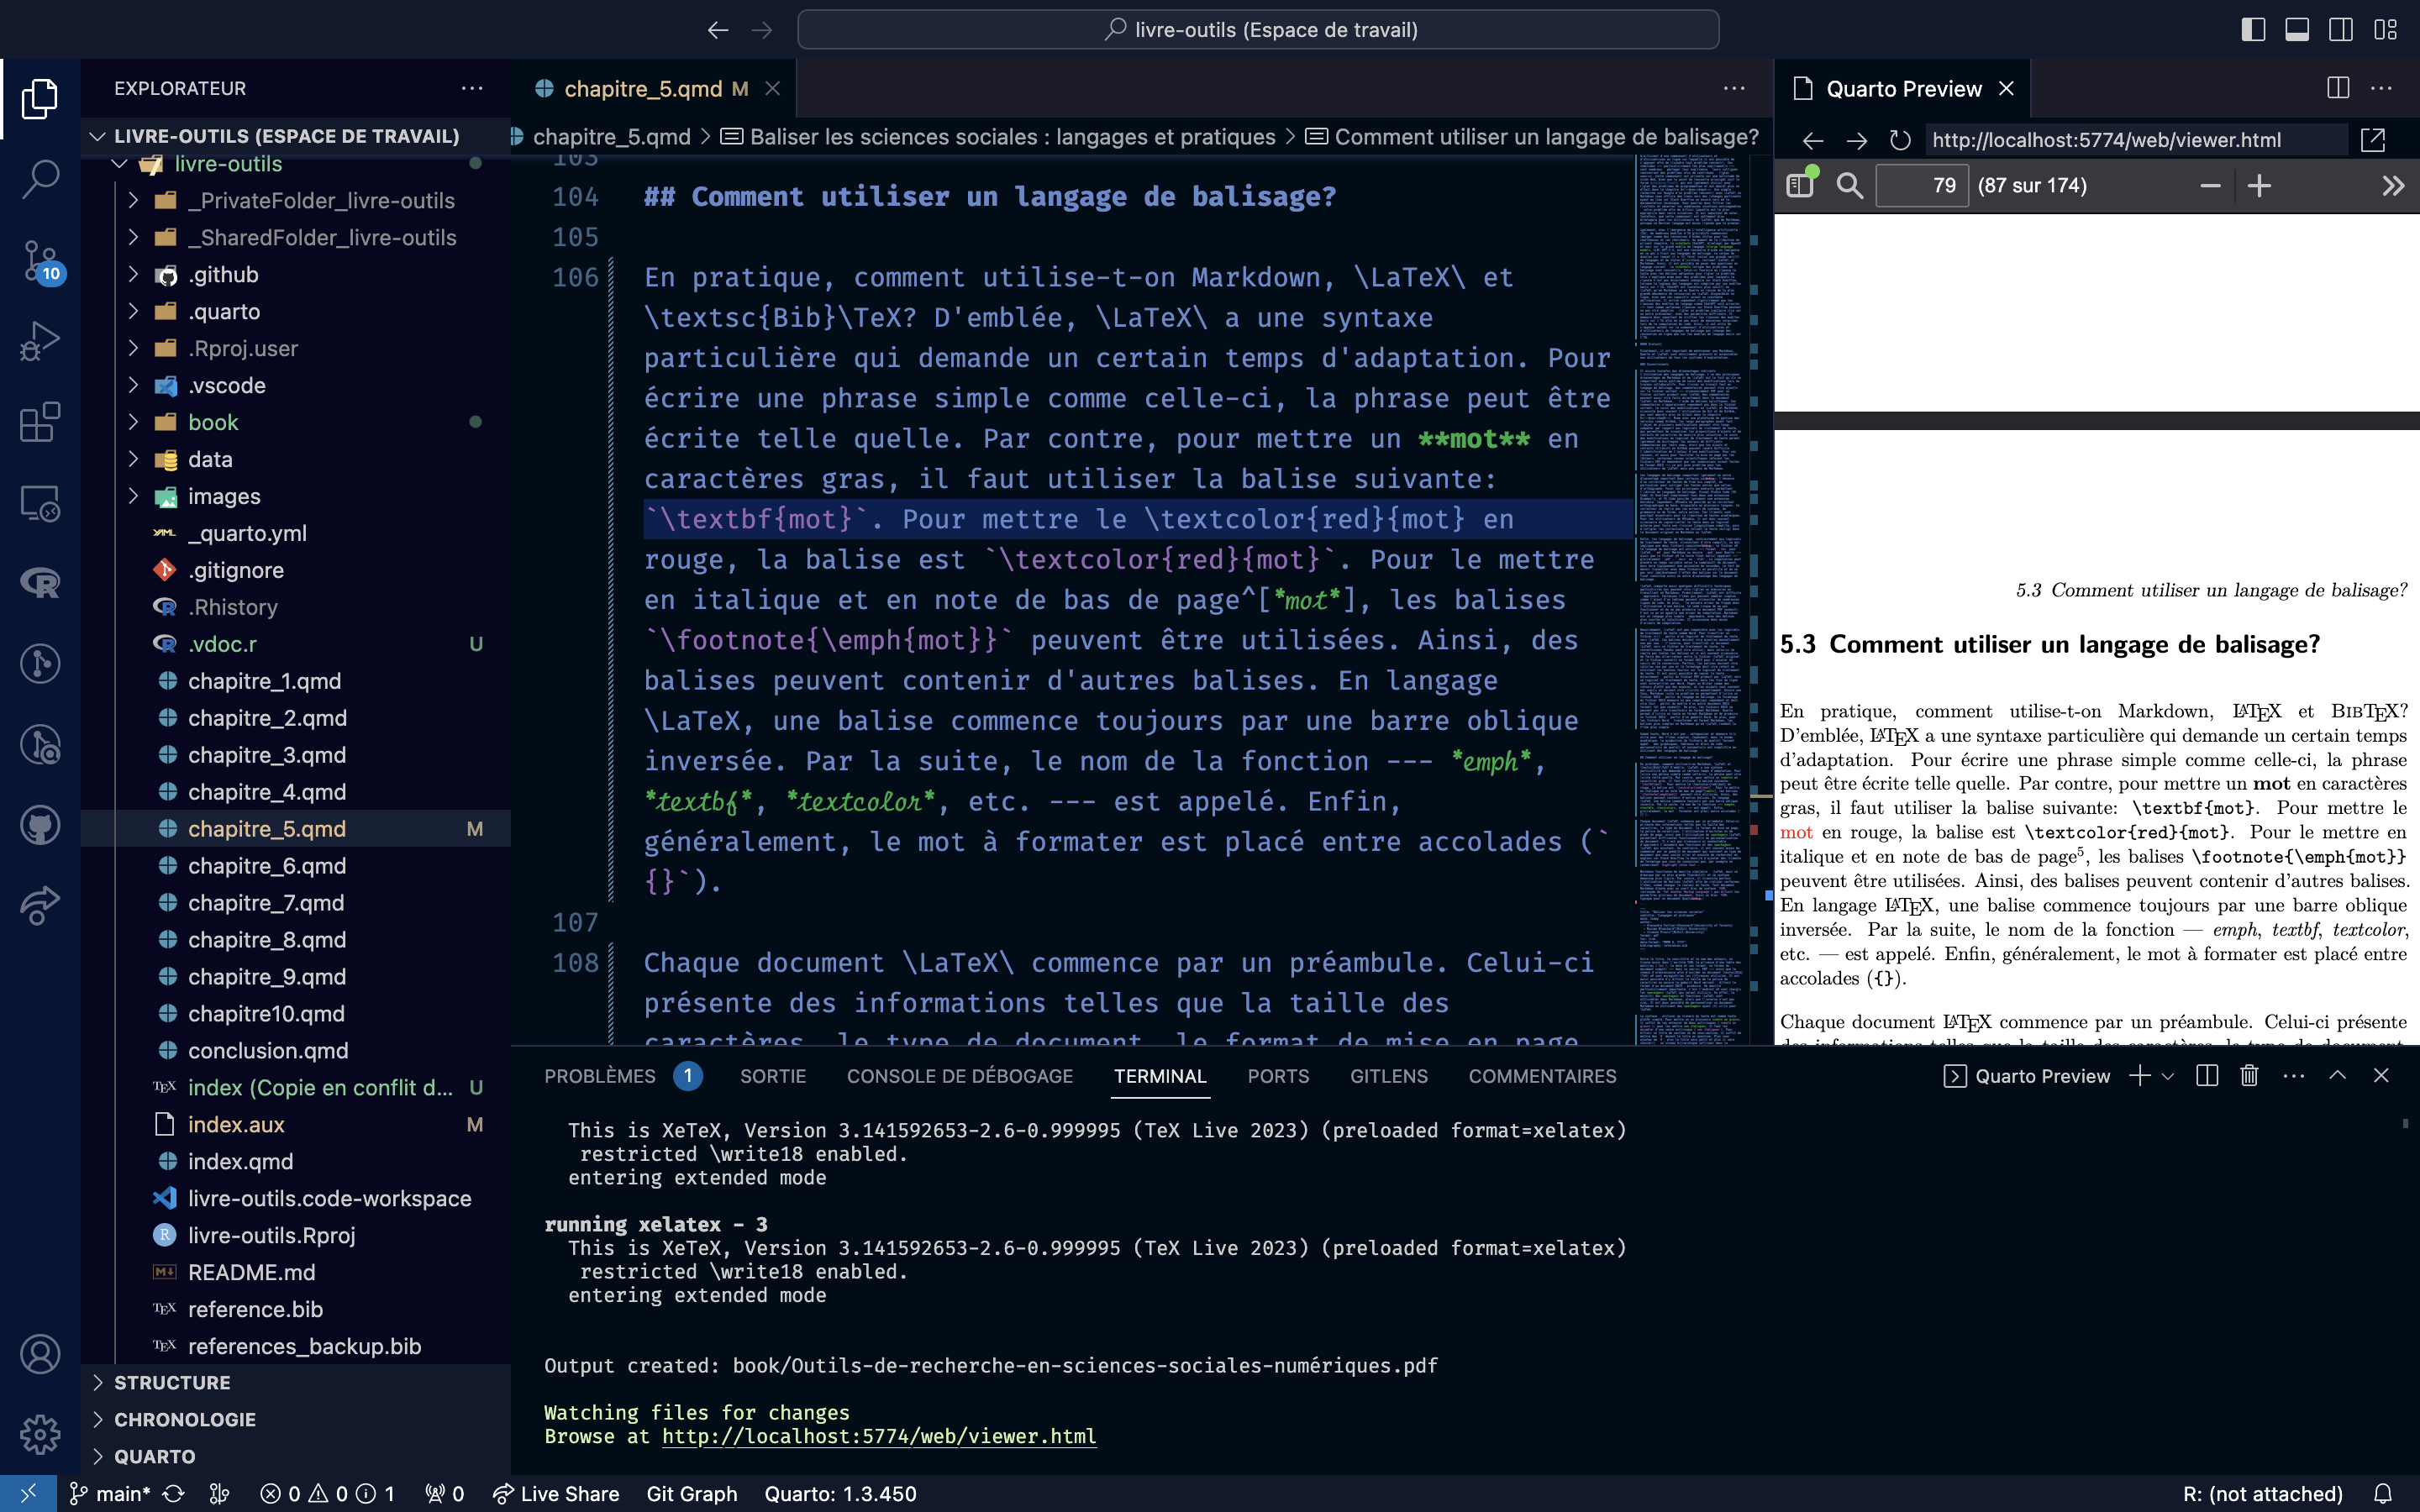
\includegraphics[width=4.8in,height=\textheight]{images/chapitre5_vscode.png}

}

\caption{\label{fig-vscode}Exemple d'utilisation du langage de balisage
Markdown dans un fichier Quarto sur la plateforme VS Code newline
\emph{Source}~: Auteurs du présent chapitre.}

\end{figure}%

Le premier langage de balisage, le Generalized Markup Language (GML), a
été inventé en 1969 par les chercheurs Charles F. Goldfarb, Ed Mosher et
Ray Lorie pour la compagnie IBM. Goldfarb et ses collègues devaient
intégrer trois applications créées avec des langages différents et avec
une logique différente pour les besoins d'un bureau de droit. Même après
avoir créé un programme qui permettait aux trois applications
d'interagir, ces langages demeuraient différents et avaient chacun leur
propre fonctionnement. Le développement de GML a permis de résoudre ce
problème en standardisant et en structurant le langage~: les mêmes
commandes étaient utilisées pour accomplir les mêmes tâches dans chaque
programme (\textbf{goldfarbRootsSGMLPersonal1996?}). GML a été amélioré
durant les décennies suivantes et a été suivi par d'autres langages de
balisage, dont LaTeX (1985), \textsc{Bib}TeX (1988), HTML (1993), XML
(1998), Markdown (2004) et \texttt{R} Markdown (2012) (Extensible
{Markup Language} ({XML}) 1.0, 1998, Getting {Started}, 2023, {HTML
History} \textbar{} {Explained}, 2023, {LaTeX}, 2023, Markdown, 2023).

Les langages de balisage permettent d'effectuer différentes tâches.
HTML, qui est sans doute le plus connu des langages de balisage, permet
de formater des sites Web. XML, quant à lui, permet de structurer de
larges volumes de données. LaTeX permet pour sa part de formater du
texte et de créer des documents en format PDF. Markdown permet également
de créer des documents en format PDF, mais aussi en format HTML ou DOCX
--- format utilisé pour les documents Word ---, contrairement à LaTeX.
\texttt{R} Markdown permet d'ajouter des extraits de code \texttt{R} à
un fichier en langage Markdown. Enfin, depuis 2022, le système de
publication scientifique et technique multilingue Quarto permet de créer
des documents qui intègrent des extraits de code \texttt{R}, LaTeX,
Python, Julia ou JavaScript, créés dans différents types
d'environnements, à un fichier en langage Markdown
(\textbf{allaire22?}). LaTeX, Markdown, \texttt{R} Markdown et Quarto
permettent aussi d'intégrer les références bibliographiques du système
de traitement de références \textsc{Bib}TeX. Les langages de balisage
communiquent ainsi souvent les uns avec les autres au sein d'un même
fichier. Le chapitre 6 explique la manière de citer les références en
langage \textsc{Bib}TeX par le biais de Zotero et de Better
\textsc{Bib}TeX.

Les balises constituent une manière de donner manuellement des commandes
au logiciel que vous utilisez. Si vous utilisez Microsoft Word, vous
avez accès à une panoplie de boutons qui vous permettent de formater
votre texte. Les balises exercent les mêmes fonctions de formatage pour
les fichiers produits en LaTeX ou en Markdown, mais doivent être
ajoutées à l'écrit par l'utilisateur. Lorsque vous appuyez sur un bouton
ou utilisez une commande comme \texttt{Ctrl-G} ou \texttt{Cmd-I} dans
Word, en réalité, cette commande ajoute des balises au travers de votre
texte, mais rend celles-ci invisibles dans l'interface que vous
utilisez. Cela permet d'avoir un texte élégant et facile à lire, mais
comporte aussi plusieurs inconvénients. Le principal inconvénient est de
limiter le pouvoir que vous avez sur le formatage de votre texte. En
effet, si les boutons à votre disposition ne vous permettent pas de
réaliser une opération, celle-ci sera éternellement impossible à
réaliser pour vous. A contrario, les langages de balisage permettent un
contrôle presque infini sur les opérations que vous souhaitez réaliser.
Incidemment, dans la mesure où vous utilisez le langage approprié pour
la tâche que vous souhaitez accomplir, vous devriez être capable de
donner exactement la commande nécessaire à votre logiciel. Les langages
de balisage, bien qu'ils aient un coût d'apprentissage qui peut s'avérer
important et que l'interface de travail soit moins intuitive qu'un
document Word, vous offrent une plus grande flexibilité.

Afin d'utiliser un langage de balisage, il est impératif que le logiciel
que vous utilisez puisse prendre en compte ce langage. Un logiciel
permet rarement d'utiliser n'importe quel langage. Par exemple, le
logiciel \TeX{}Shop permet seulement d'utiliser le langage LaTeX. Il est
aussi impératif de bien utiliser le langage de balisage. En effet, comme
pour les langages de programmation, les langages de balisage ne peuvent
pas déduire ce que vous souhaitez leur faire comprendre. Si vous
souhaitez mettre du texte en gras, vous devez utiliser les bonnes
balises. La moindre erreur peut être coûteuse, puisqu'une erreur dans la
balise que vous utilisez risque de produire une commande
incompréhensible et un message d'erreur, le logiciel ne réussissant pas
à associer votre balise mal inscrite à une action informatisée.
Conséquemment, il est impératif de bien vérifier les balises utilisées
afin d'éviter toute erreur qui empêcherait votre document d'être
compilé, c'est-à-dire d'être traduit dans son format final\footnote{Les
  logiciels permettent plus ou moins efficacement d'identifier les
  balises problématiques. Certains ne produisent qu'un message d'erreur
  sans donner d'indication sur la source du problème, alors que d'autres
  ciblent très spécifiquement la ligne de syntaxe où se situe la balise
  problématique.}. Chaque caractère dans une balise est important et il
y a rarement plus d'une seule manière de commander une action. Par
exemple, en LaTeX, il n'y a qu'une seule manière de mettre du texte en
gras. Il faut précisément utiliser cette commande:
\texttt{\textbackslash{}textbf\{\}}. Le positionnement des balises est
lui aussi critique~: il délimite la portion de texte à laquelle doit
être appliquée l'action commandée par la balise.

Il est important de distinguer les langages de balisage des langages de
programmation, qui sont abordés plus en détail dans le chapitre 4. En
effet, ceux-ci sont similaires à certains égards, mais ont des vocations
différentes. Les deux s'appuient sur un langage informatisé, mais les
langages et leurs objectifs diffèrent. Un langage de programmation
définit des processus informatisés alors qu'un langage de balisage
permet d'encoder du contenu de manière à ce que celui-ci soit lisible
tant pour l'humain que pour son ordinateur.

Dans le contexte de la recherche en sciences sociales, la programmation
est généralement utilisée afin de récolter, d'analyser et de présenter
visuellement des données. Une fois cartes, tableaux et graphiques
produits, ceux-ci peuvent être enregistrés --- par exemple en format PDF
ou PNG --- et inclus au sein d'un document qui sera formaté en utilisant
un langage de balisage. En \texttt{R} Markdown et en Quarto, des
extraits de langage de programmation peuvent être inclus dans des
sections bien délimitées de documents écrits en langage de balisage.
Plus généralement, le langage de programmation contribue à l'analyse
alors que le langage de balisage est essentiellement utile afin de
présenter les travaux de recherche, que ce soit dans un document écrit
ou sur un site Web. C'est principalement de cette manière que sont
utilisés les langages de programmation et de balisage dans le cadre de
la recherche en sciences sociales.

\section{Comment utiliser un langage de
balisage?}\label{comment-utiliser-un-langage-de-balisage}

En pratique, comment utilise-t-on Markdown, LaTeX et \textsc{Bib}TeX?
D'emblée, LaTeX a une syntaxe particulière qui demande un certain temps
d'adaptation. Pour écrire une phrase simple comme celle-ci, la phrase
peut être écrite telle quelle. Par contre, pour mettre un \textbf{mot}
en caractères gras, il faut utiliser la balise suivante:
\texttt{\textbackslash{}textbf\{mot\}}. Pour mettre le
\textcolor{red}{mot} en rouge, la balise est
\texttt{\textbackslash{}textcolor\{red\}\{mot\}}. Pour le mettre en
italique et en note de bas de page\footnote{\emph{mot}}, les balises
\texttt{\textbackslash{}footnote\{\textbackslash{}emph\{mot\}\}} peuvent
être utilisées. Ainsi, des balises peuvent contenir d'autres balises. En
langage LaTeX, une balise commence toujours par une barre oblique
inversée. Par la suite, le nom de la fonction --- \emph{emph},
\emph{textbf}, \emph{textcolor}, etc. --- est appelé. Enfin,
généralement, le mot à formater est placé entre accolades
(\texttt{\{\}}).

Chaque document \LaTeX{} commence par un préambule. Celui-ci présente
des informations telles que la taille des caractères, le type de
document, le format de mise en page, la police de caractères,
l'utilisation d'en-têtes et de pieds de page, ainsi que l'utilisation de
\emph{packages} LaTeX permettant différentes fonctionnalités de
personnalisation du document. Il n'est pas nécessaire ni souhaitable
d'apprendre l'ensemble des fonctions et des \emph{packages} LaTeX qui
existent. Au contraire, il est souvent mieux de commencer par un gabarit
de document qui convient au type de document que vous voulez créer et
ensuite de rechercher en anglais sur Stack Overflow la manière d'ajouter
des éléments de formatage que vous ne connaissez pas, par exemple en
recherchant \texttt{highlight\ latex\ text}.

Markdown fonctionne de manière similaire à LaTeX, mais se démarque par
sa plus grande flexibilité et sa syntaxe beaucoup plus légère. Par
contre, il nécessite parfois l'utilisation de balises LaTeX afin de
réaliser certaines tâches, comme changer la couleur du texte. Tout
document Markdown débute avec un court bloc de syntaxe \texttt{YAML}
(acronyme de \texttt{Yet\ Another\ Markup\ Language}) qui définit les
paramètres généraux du document. Voici un bloc \texttt{YAML} typique
pour un document Quarto~:

\begin{verbatim}
---
title: "Baliser les sciences sociales"
subtitle: "Langages et pratiques"
date: today
author:
  - Alexandre Fortier-Chouinard^[University of Toronto]
  - Étienne Proulx^[McGill University]
  - Maxime Blanchard^[McGill University]
format: pdf
toc: true
date-format: "MMMM D, YYYY"
bibliography: livre-outils.bib
---
\end{verbatim}

Outre le titre, le sous-titre et le nom des auteurs, on trouve aussi
dans l'en-tête YAML la présence d'une table des matières (\texttt{toc}),
la date et son format, le format du document compilé --- dans ce cas-ci,
PDF --- ainsi que le chemin d'arborescence afin d'accéder au document
\textsc{Bib}TeX où sont enregistrées les références utilisées. Il est
aussi possible d'y définir la taille de la police de caractères ou
encore le gabarit Word servant à définir le format d'un document DOCX à
produire. De manière particulièrement importante, c'est l'endroit où
sont chargés les \emph{packages} LaTeX qui seront utilisés. En effet, la
majorité des \emph{packages} et fonctions LaTeX sont utilisables dans
Markdown, alors que l'inverse n'est pas vrai. Il est donc possible de
personnaliser un document Markdown en utilisant des \emph{packages}
ayant été créés pour LaTeX.

La syntaxe à utiliser au travers du texte est somme toute plutôt simple.
Pour mettre un ou plusieurs \textbf{mots en gras}, il suffit de les
entourer de deux astérisques (\texttt{**mots\ en\ gras**}); pour les
mettre \emph{en italique}, il faut les encadrer d'une seule astérisque
(\texttt{*en\ italique*}). Pour définir un titre de section ou de
sous-section, il suffit de mettre des \texttt{\#} devant le titre en
question. Plus vous ajoutez de \texttt{\#}, plus le titre sera petit et
plus il sera considéré à un niveau hiérarchique inférieur dans la
structure du texte. La syntaxe Markdown est donc plus légère que celle
de LaTeX, dans le but d'en rendre la lecture plus simple pour les
utilisateurs et utilisatrices.

Bien que des gabarits Markdown soient disponibles, ceux-ci sont plus
rares. Ils se trouvent pour la plupart sur GitHub et sont rendus
disponibles par leur créateur. Cela étant dit, leur personnalisation
peut s'avérer plutôt complexe. En somme, Markdown est particulièrement
pratique pour les documents ne nécessitant pas de respecter un gabarit
précis et requérant simplement un document d'allure simple et
professionnelle.

Pour sa part, \textsc{Bib}TeX a une syntaxe relativement simple.
D'emblée, les références \textsc{Bib}TeX pour des articles et ouvrages
scientifiques sont disponibles sur Google Scholar. Toutefois, pour citer
des sites Web ou des articles de médias, la référence doit être écrite à
la main selon un format précis. Une bibliographie sur \textsc{Bib}TeX
peut ressembler à ceci~:

\begin{verbatim}
@book{darwin03,
  address = {London},
  author = {Darwin, Charles},
  publisher = {John Murray},
  title = {{On the Origin of Species by Means of Natural Selection
or the Preservation of Favoured Races in the Struggle for Life}},
  year = {1859}
}

@article{goldfarb96,
  title={The Roots of SGML: A Personal Recollection},
  author={Goldfarb, Charles F},
  journal={Technical communication},
  volume={46},
  number={1},
  pages={75},
  year={1999},
  publisher={Society for Technical Communication}
}
\end{verbatim}

Un fichier \textsc{Bib}TeX ne contient rien de plus qu'une série de
publications commençant chacune par la balise \texttt{@} suivie du type
d'article --- \emph{article}, \emph{book} pour un livre,
\emph{incollection} pour un chapitre de livre, \emph{inproceedings} pour
une présentation dans une conférence, \emph{unpublished} pour un article
non publié et \emph{online} pour un site Web sont parmi les plus connus
--- et des informations sur la publication mises entre accolades. La
première information entre accolades est le code de la référence, par
exemple \texttt{goldfarb96}. Dans le fichier LaTeX, l'auteur doit écrire
\texttt{\textbackslash{}cite\{goldfarb96\}} pour voir dans le document
PDF compilé (\textbf{goldfarbRootsSGMLPersonal1996?}); le lien est
automatiquement cliquable et renvoie à la notice bibliographique
correspondante. L'ordre des publications dans le document
\textsc{Bib}TeX a peu d'importance, puisque LaTeX réordonne par défaut
la bibliographie en ordre alphabétique.

\subsection{Environnements d'édition et de
compilation}\label{environnements-duxe9dition-et-de-compilation}

Contrairement à Microsoft Word et Apple Pages, il existe plusieurs
options d'environnements d'édition et de compilation spécifiques à
chaque langage. Ces environnements sont des plateformes et des logiciels
conçus pour faciliter l'édition, la mise en forme et la compilation de
documents dans des langages de balisage tels que LaTeX et Markdown. Ils
permettent également de rendre plus efficace et conviviale la production
de documents tout en fournissant des fonctionnalités spécifiques aux
besoins de chaque langage. Il existe une grande diversité
d'environnements d'édition et de compilation, et le choix est libre pour
la chercheuse ou le chercheur de trouver celui qui convient le mieux à
ses besoins ou aux besoins de son groupe de recherche. Les trois options
discutées ici sont parmi les plus utilisées par les chercheurs en
sciences sociales et peuvent être regroupées en deux catégories~: les
logiciels de bureau et les éditeurs en ligne.

D'abord, il existe plusieurs logiciels de bureau qui offrent un
environnement d'édition et/ou de compilation pour les langages de
balisage. Ces logiciels fournissent les programmes principaux, les
extensions essentielles et des outils complémentaires de compilation et
de visualisation afin de permettre la production de documents écrits en
langages de balisage. Le logiciel RStudio, également abordé dans le
chapitre 4, permet de produire des documents avec différents langages de
balisage et programmation, ainsi que de naviguer entre eux, à partir
d'une même fenêtre. Il suffit d'installer certains \emph{packages}
contenant les fichiers nécessaires à l'utilisation des langages de
balisage. Par exemple, il est possible de produire des documents en
LaTeX en utilisant le code suivant dans la console pour installer le
\emph{package} nécessaire à l'utilisation de la distribution LaTeX
TinyTeX~: \texttt{install.packages("tinytex")}. Suivant le même
principe, il est possible de produire des documents en \texttt{R}
Markdown sur RStudio en installant le \emph{package} suivant~:
\texttt{install.packages("rmarkdown")}. Pour Quarto, le téléchargement
se fait en ligne, directement à partir du site Web de (Get {Started},
2023).

Pour l'écriture en LaTeX, il est également nécessaire d'installer l'une
des nombreuses distributions en ligne afin de pouvoir compiler ces
documents dans un environnement local. Il existe des distributions
telles que MacTeX pour Mac, MikTeX pour Windows et plusieurs autres
(Just, 2013). Ces distributions se distinguent par les différents
\emph{packages} avec lesquelles elles sont compatibles.

Un autre environnement régulièrement utilisé pour travailler en langage
de balisage est le logiciel de bureau VS Code. VS Code prend en compte
un plus grand nombre de langages de programmation et est utilisé par les
programmeurs de tous domaines, tandis qu'RStudio est surtout utile pour
les chercheurs en sciences sociales qui travaillent surtout en
\texttt{R}.

Lorsque vient le temps de collaborer à plusieurs sur un document écrit
en Markdown ou en LaTeX, les logiciels de bureau évoqués précédemment
nécessitent l'utilisation de GitHub et de Git. L'utilisation de ces
éditeurs peut présenter un défi supplémentaire pour les équipes de
recherche non initiées. Il existe ainsi des éditeurs en ligne qui
permettent de collaborer en temps réel sans passer par Git et GitHub, de
manière similaire à Google Docs\footnote{VS Code possède également une
  extension, Live Share, qui permet de travailler en temps réel sur un
  même document.}. Le plus connu de ces logiciels est Overleaf, qui
permet de produire des documents en langage LaTeX. Puisqu'Overleaf
permet d'avoir accès à ses documents LaTeX à partir de n'importe quel
navigateur, il n'y a pas de dépendance à un logiciel local sur un
ordinateur, ce qui constitue un avantage important. La contrepartie de
cet avantage est qu'en utilisant Overleaf, l'équipe de recherche est
dépendante d'une connexion à Internet. En utilisant le package LaTeX
\texttt{rmarkdown}, Overleaf peut également inclure du code Markdown.
Cependant, Overleaf ne permet pas de créer des documents en format DOCX
ou HTML, ce qui constitue une limite de l'application. Overleaf comporte
un compteur de mots intégré, ce qui n'est pas le cas des autres
logiciels et environnements présentés plus haut.

\section{Quand et pourquoi utiliser un langage de
balisage?}\label{quand-et-pourquoi-utiliser-un-langage-de-balisage}

La plupart des langages de balisage permettent de remplir l'une des deux
fonctions suivantes, qui sont particulièrement importantes dans le
contexte de la recherche en sciences sociales~: produire des documents
écrits et formater des pages Web. Dans les deux cas, ces actions peuvent
être réalisées à partir de logiciels simples, mais ces logiciels ont des
limites importantes auxquelles les langages de balisage apportent des
solutions\footnote{Les langages de balisage permettent également de
  créer des pages Web. Bien que les pages Web puissent être créées à
  partir de sites Web comme WordPress, le langage HTML permet de
  produire des résultats plus \emph{personnalisables}, plus
  \emph{automatisables} et avec une plus \emph{grande qualité
  graphique}. Cette question n'est pas abordée en détail dans ce
  chapitre.}.

Pour l'écriture de documents très simples comme une liste d'épicerie ou
des notes rapides pendant une conférence, les logiciels de traitement de
texte sont tout à fait convenables~: ils sont simples et rapides à
utiliser, un formatage professionnel du document n'est pas de mise.
Utiliser un langage de balisage pour des tâches de base peut en effet
rendre la tâche inutilement longue et complexe. Toutefois, plus la
complexité d'un document augmente, plus il devient difficile d'obtenir
un résultat satisfaisant en utilisant un logiciel de traitement de texte
tel que Word, Pages ou Writer. A contrario, LaTeX permet de produire des
documents de tous les niveaux de complexité, tel que démontré sur la
Figure~\ref{fig-latex-vs-word}. Quant à Markdown, sa courbe
d'apprentissage se situerait logiquement entre celles de LaTeX et de
Word, puisque ses balises sont simplifiées. Plus généralement, utiliser
un langage de balisage comme LaTeX ou Markdown\footnote{Les avantages et
  désavantages de Markdown cités dans cette section s'appliquent
  également à Quarto et à \texttt{R} Markdown, puisque ces derniers font
  appel au langage Markdown.} comporte plusieurs avantages par rapport
aux logiciels de traitement de texte traditionnels. Ces avantages font
tous appel à un mélange de quatre concepts principaux~: automatisation,
personnalisation, flexibilité et qualité graphique.

\begin{figure}

\centering{

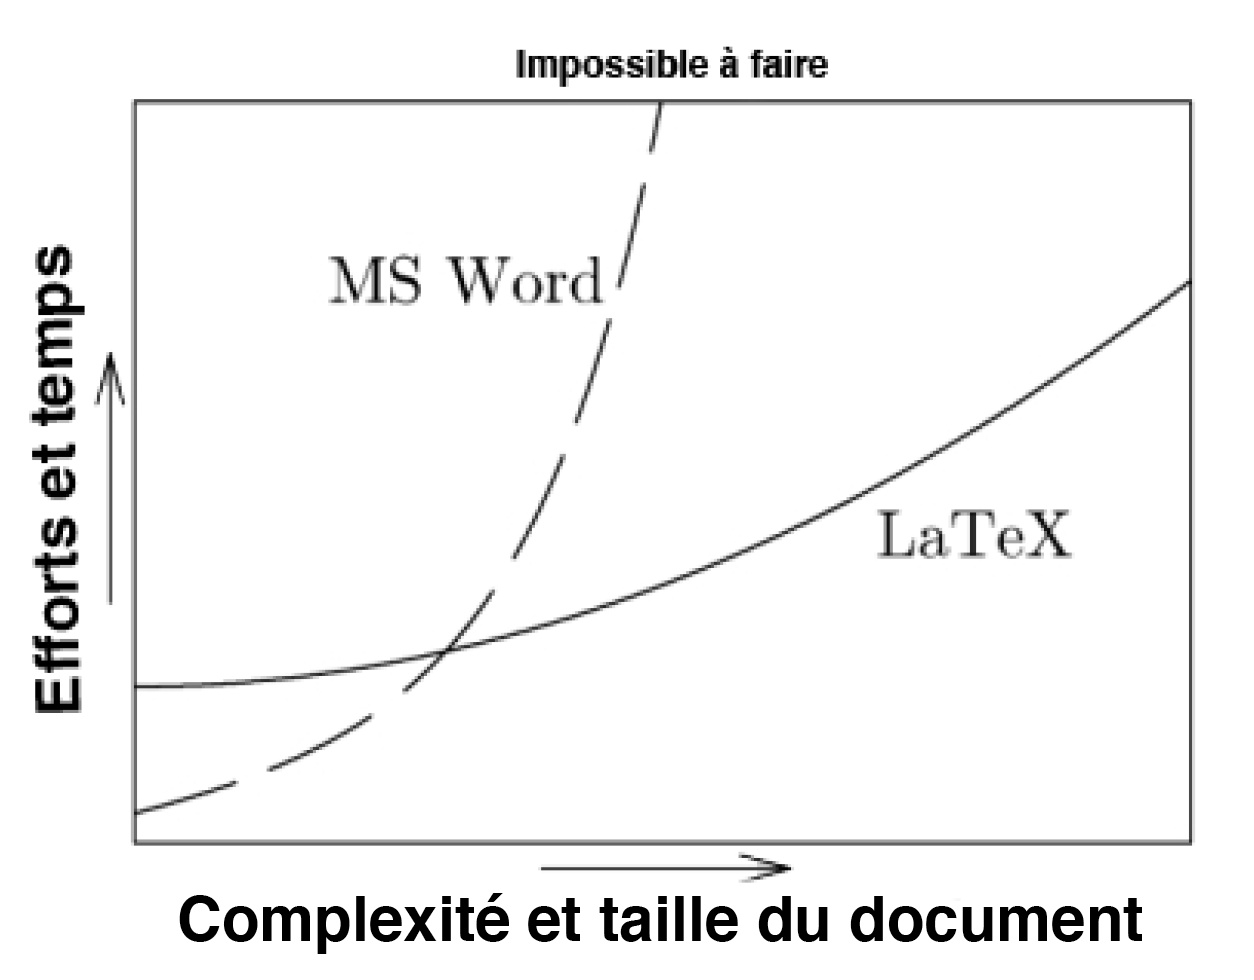
\includegraphics[width=4.18in,height=\textheight]{images/chapitre5_word-vs-latex.png}

}

\caption{\label{fig-latex-vs-word}Utilité relative de Word et de LaTeX
selon la complexité et la taille du document \emph{Source}~: Yannick
Dufresne (2015).}

\end{figure}%

\subsection{Avantages}\label{avantages-3}

\subsubsection{Référencement}\label{ruxe9fuxe9rencement}

Premièrement, LaTeX et Markdown permettent d'intégrer une bibliographie
\emph{automatique} et professionnelle en utilisant \textsc{Bib}TeX.
Cette bibliographie peut être adaptée très facilement en différents
styles bibliographiques reconnus ou en un style bibliographique
\emph{personnalisé} à partir d'un des nombreux gabarits professionnels
disponibles. Avec \textsc{Bib}TeX, il n'y a pas à vérifier si le titre
de l'article est toujours en italique, si le numéro de volume est
toujours entre parenthèses ou si le nom de famille des deuxièmes auteurs
est toujours avant ou après le prénom puisque toutes ces opérations sont
effectuées de manière \emph{automatique}. \textsc{Bib}TeX comprend
également les différences entre les types de sources --- articles
scientifiques, livres, sites Internet, etc. --- et ajuste leur
présentation en conséquence. De plus, si une des sources que vous citez
n'est pas incluse dans la bibliographie, une erreur s'affiche, vous
permettant d'identifier le problème plutôt que de vous retrouver avec
une référence manquante. À l'inverse, si une source est retirée du
texte, elle disparait \emph{automatiquement} de la bibliographie dans le
document final mais demeure présente dans le fichier où se trouvent les
références bibliographiques. Cela évite les aller-retour pour vérifier
que chaque source de la bibliographie se trouve au moins une fois dans
le texte et que chaque source dans le texte est citée en bibliographie.
Grâce aux balises, en cliquant sur les références incluses dans le
document, vous vous retrouverez immédiatement plus loin dans le
document, à l'endroit où se trouve l'entrée bibliographique associée.
Les références \textsc{Bib}TeX pour articles scientifiques peuvent être
copiées-collées à partir de Google Scholar. \textsc{Bib}TeX rend donc
extrêmement simple et efficace l'utilisation des références
bibliographiques grâce à sa capacité à \emph{personnaliser} et
\emph{automatiser} leur présentation\footnote{L'utilisation d'un
  logiciel de traitement de texte, en particulier lorsque combiné avec
  une extension Zotero, peut également produire un résultat automatisé
  et personnalisé à un certain degré. Cependant, au moment où ce
  chapitre est écrit, le retrait d'une citation du texte principal en
  Word avec Zotero n'enlève pas immédiatement cette citation de la
  bibliographie, et l'ajout de liens vers la bibliographie doit se faire
  source par source, ce qui prend un temps important et peut occasionner
  des erreurs humaines.}.

\subsubsection{Figures et tableaux}\label{figures-et-tableaux}

L'intégration de figures et de tableaux dans le texte est aussi rendue
très simple et professionnelle grâce à LaTeX et à Markdown. La taille de
la figure ou du tableau, son positionnement et son intégration par
rapport au texte environnant peuvent être réglés avec précision.
Cependant, l'ajout de texte avant ou après la figure ou le tableau ne
produira pas des résultats inattendus tels qu'une demi-page vide avant
un graphique ou un titre de tableau complètement en bas d'une page. En
définissant des paramètres pour l'ensemble du texte, la chercheuse ou le
chercheur peut \emph{personnaliser} entièrement la présentation des
figures et des tableaux. De plus, la \emph{qualité des figures et des
tableaux} ne diminue pas lors de leur intégration~: les figures restent
aussi belles qu'elles l'étaient originalement, ce qui n'est pas toujours
le cas dans les logiciels de traitement de texte. Les figures et les
tableaux sont aussi numérotés \emph{automatiquement}, ce qui veut dire
que vous n'aurez jamais à vous préoccuper de modifier les numéros si
l'ordre des figures et tableaux est modifié dans le texte. Grâce aux
balises, en cliquant sur le numéro associé à la figure ou au tableau
dans le texte, le document se retrouve automatiquement à l'endroit où se
trouve la figure ou le tableau. De plus, les figures peuvent être
intégrées en format PDF, ce qui permet au lecteur de copier-coller ou de
surligner de l'information se trouvant sur le graphique directement,
incluant les titres des axes et les annotations.

Surtout, l'intégration de graphiques produits par \texttt{R} au texte en
langage de balisage est simplifiée et \emph{automatisée}. En effet, même
lorsque les données ou le code pour produire un graphique changent,
\texttt{R} resauvegarde le fichier dans le même chemin d'arborescence
(\emph{path}) particulier que vous avez indiqué, par exemple
\texttt{C:/Users/Jean/Dropbox/projet1/graphs/Figure1.pdf}. Le langage de
balisage peut ensuite indiquer le même chemin d'arborescence, de sorte
qu'il n'est pas nécessaire de recopier-coller la figure à l'intérieur du
document chaque fois que des changements y sont apportés; la figure est
mise à jour \emph{automatiquement}.

L'intégration de figures et de tableaux est particulièrement simple et
\emph{flexible} avec Quarto. Contrairement à LaTeX, qui nécessite la
production de tableaux et de figures dans un document en langage de
programmation (comme \texttt{R}), Quarto permet de créer une figure
grâce à du code \texttt{R} \emph{et} d'intégrer celle-ci au texte dans
un même document. Cela se fait grâce à l'intégration de blocs de code
\texttt{R} (\emph{code chunks}) dans le document. Le code est produit
dans le bloc de code et la figure ou le tableau qui en résulte apparait
à la fois dans le document Quarto, où des balises supplémentaires
permettent d'adapter le formatage, et sur le document fini. Cependant,
certains \emph{packages} R permettent de créer des tableaux de
régression de grande qualité en format LaTeX. Les tableaux de régression
en format Markdown sont pour l'instant plus difficiles à produire
au-delà d'un certain niveau de complexité, en raison des limitations du
langage Markdown. Il demeure possible de produire des tableaux en
langage LaTeX dans un fichier Markdown ou Quarto.

\subsubsection{Équations}\label{uxe9quations}

LaTeX permet également d'ajouter des équations mathématiques poussées.
En effet, il existe des balises pour chaque symbole mathématique, et
celles-ci peuvent être agencées de manière à former des équations
cohérentes. Ces équations peuvent être intégrées au sein même d'une
phrase ou être mises de l'avant dans un paragraphe à part centré.

\subsubsection{Table des matières et mise en
page}\label{table-des-matiuxe8res-et-mise-en-page}

Markdown et LaTeX permettent aussi la gestion \emph{automatisée} de la
table des matières, et les références aux pages appropriées à partir de
la table des matières se mettent à jour en continu. La table des
matières prend en compte l'architecture du texte choisie manuellement
par le chercheur, qui est définie par des balises définissant différents
niveaux hiérarchiques de sections, sous-sections ou chapitres. Des
manières \emph{automatiques} de référencer les figures et les tableaux
dans des sections distinctes de la table des matières sont également
offertes, encore une fois \emph{personnalisables} au goût du chercheur.

Bien que la mise en page de documents produits via Markdown et LaTeX
puisse être définie entièrement manuellement par les personnes plus
expérimentées, les novices apprécieront les nombreux gabarits
(\emph{templates}) qui permettent de gérer \emph{automatiquement} la
mise en page clés en main. Les gabarits permettent de rendre l'apparence
d'un document plus esthétique et uniforme et peuvent être utilisés tels
quels ou servir de point de départ pour un chercheur ou une chercheuse
souhaitant y apporter certaines modifications sans toutefois partir
d'une feuille blanche. La majorité des personnes qui utilisent ces
langages, même les plus expérimentées, utilisent ces gabarits comme base
lorsqu'elles rédigent un document. Ceux-ci constituent une mine d'or
puisqu'ils rendent accessible le code Markdown ou LaTeX ayant servi à la
conception du gabarit, permettant à la chercheuse ou au chercheur de
comprendre comment est obtenu le résultat que lui offre le gabarit.
Incidemment, il est possible d'identifier les sections de code
produisant certains éléments de mise en page --- positionnement des
numéros de page, positionnement du nom des auteurs en début de document,
etc. --- et les modifier ou s'en inspirer afin de modifier d'autres
gabarits. L'utilisation de ces gabarits peut s'avérer complexe au
départ, mais il s'agit d'une complexité qui s'avère ultimement
extrêmement productive puisqu'elle vous permettra de devenir autonome et
d'ajuster les gabarits à votre convenance afin de produire exactement le
résultat désiré en termes de mise en page. En comparaison, les logiciels
de traitement de texte rendent souvent très ardue la mise en page
uniforme d'un document, puisque cet élément ne peut pas être
\emph{automatisé}. La liste des gabarits disponibles est extrêmement
large, et ceux-ci ont une variété de fonctions. En effet, une variété de
gabarits professionnels et de haute \emph{qualité graphique} sont
offerts gratuitement en ligne pour des articles, des livres, des
rapports, des \emph{curriculum vitæs} Figure~\ref{fig-cv} ou encore des
feuilles de temps pour des contrats rémunérés Figure~\ref{fig-invoice}.

\begin{figure}

\centering{

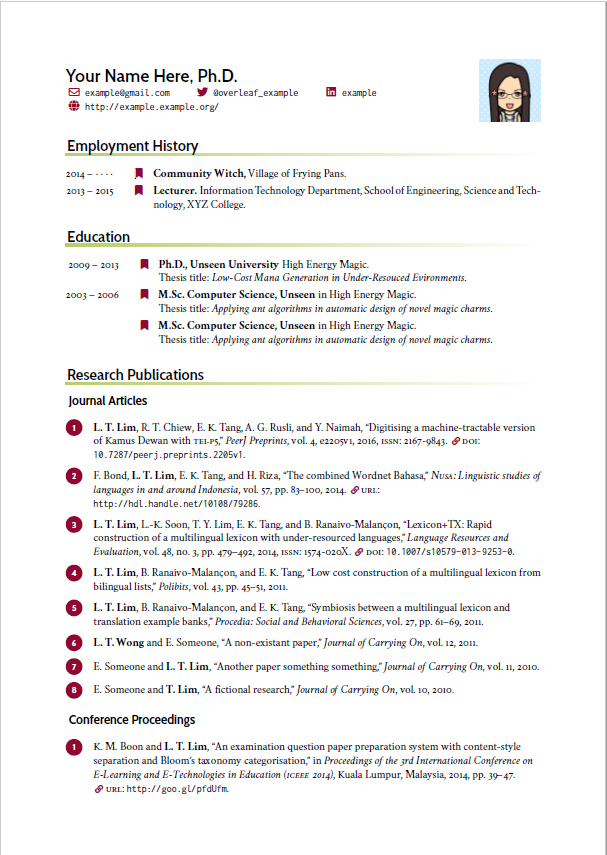
\includegraphics[width=2.02in,height=\textheight]{images/chapitre5_CVtemp.png}

}

\caption{\label{fig-cv}Exemple de gabarit LaTeX de curriculum vitae
newline \emph{Source}~: LianTze (2023).}

\end{figure}%

\begin{figure}

\centering{

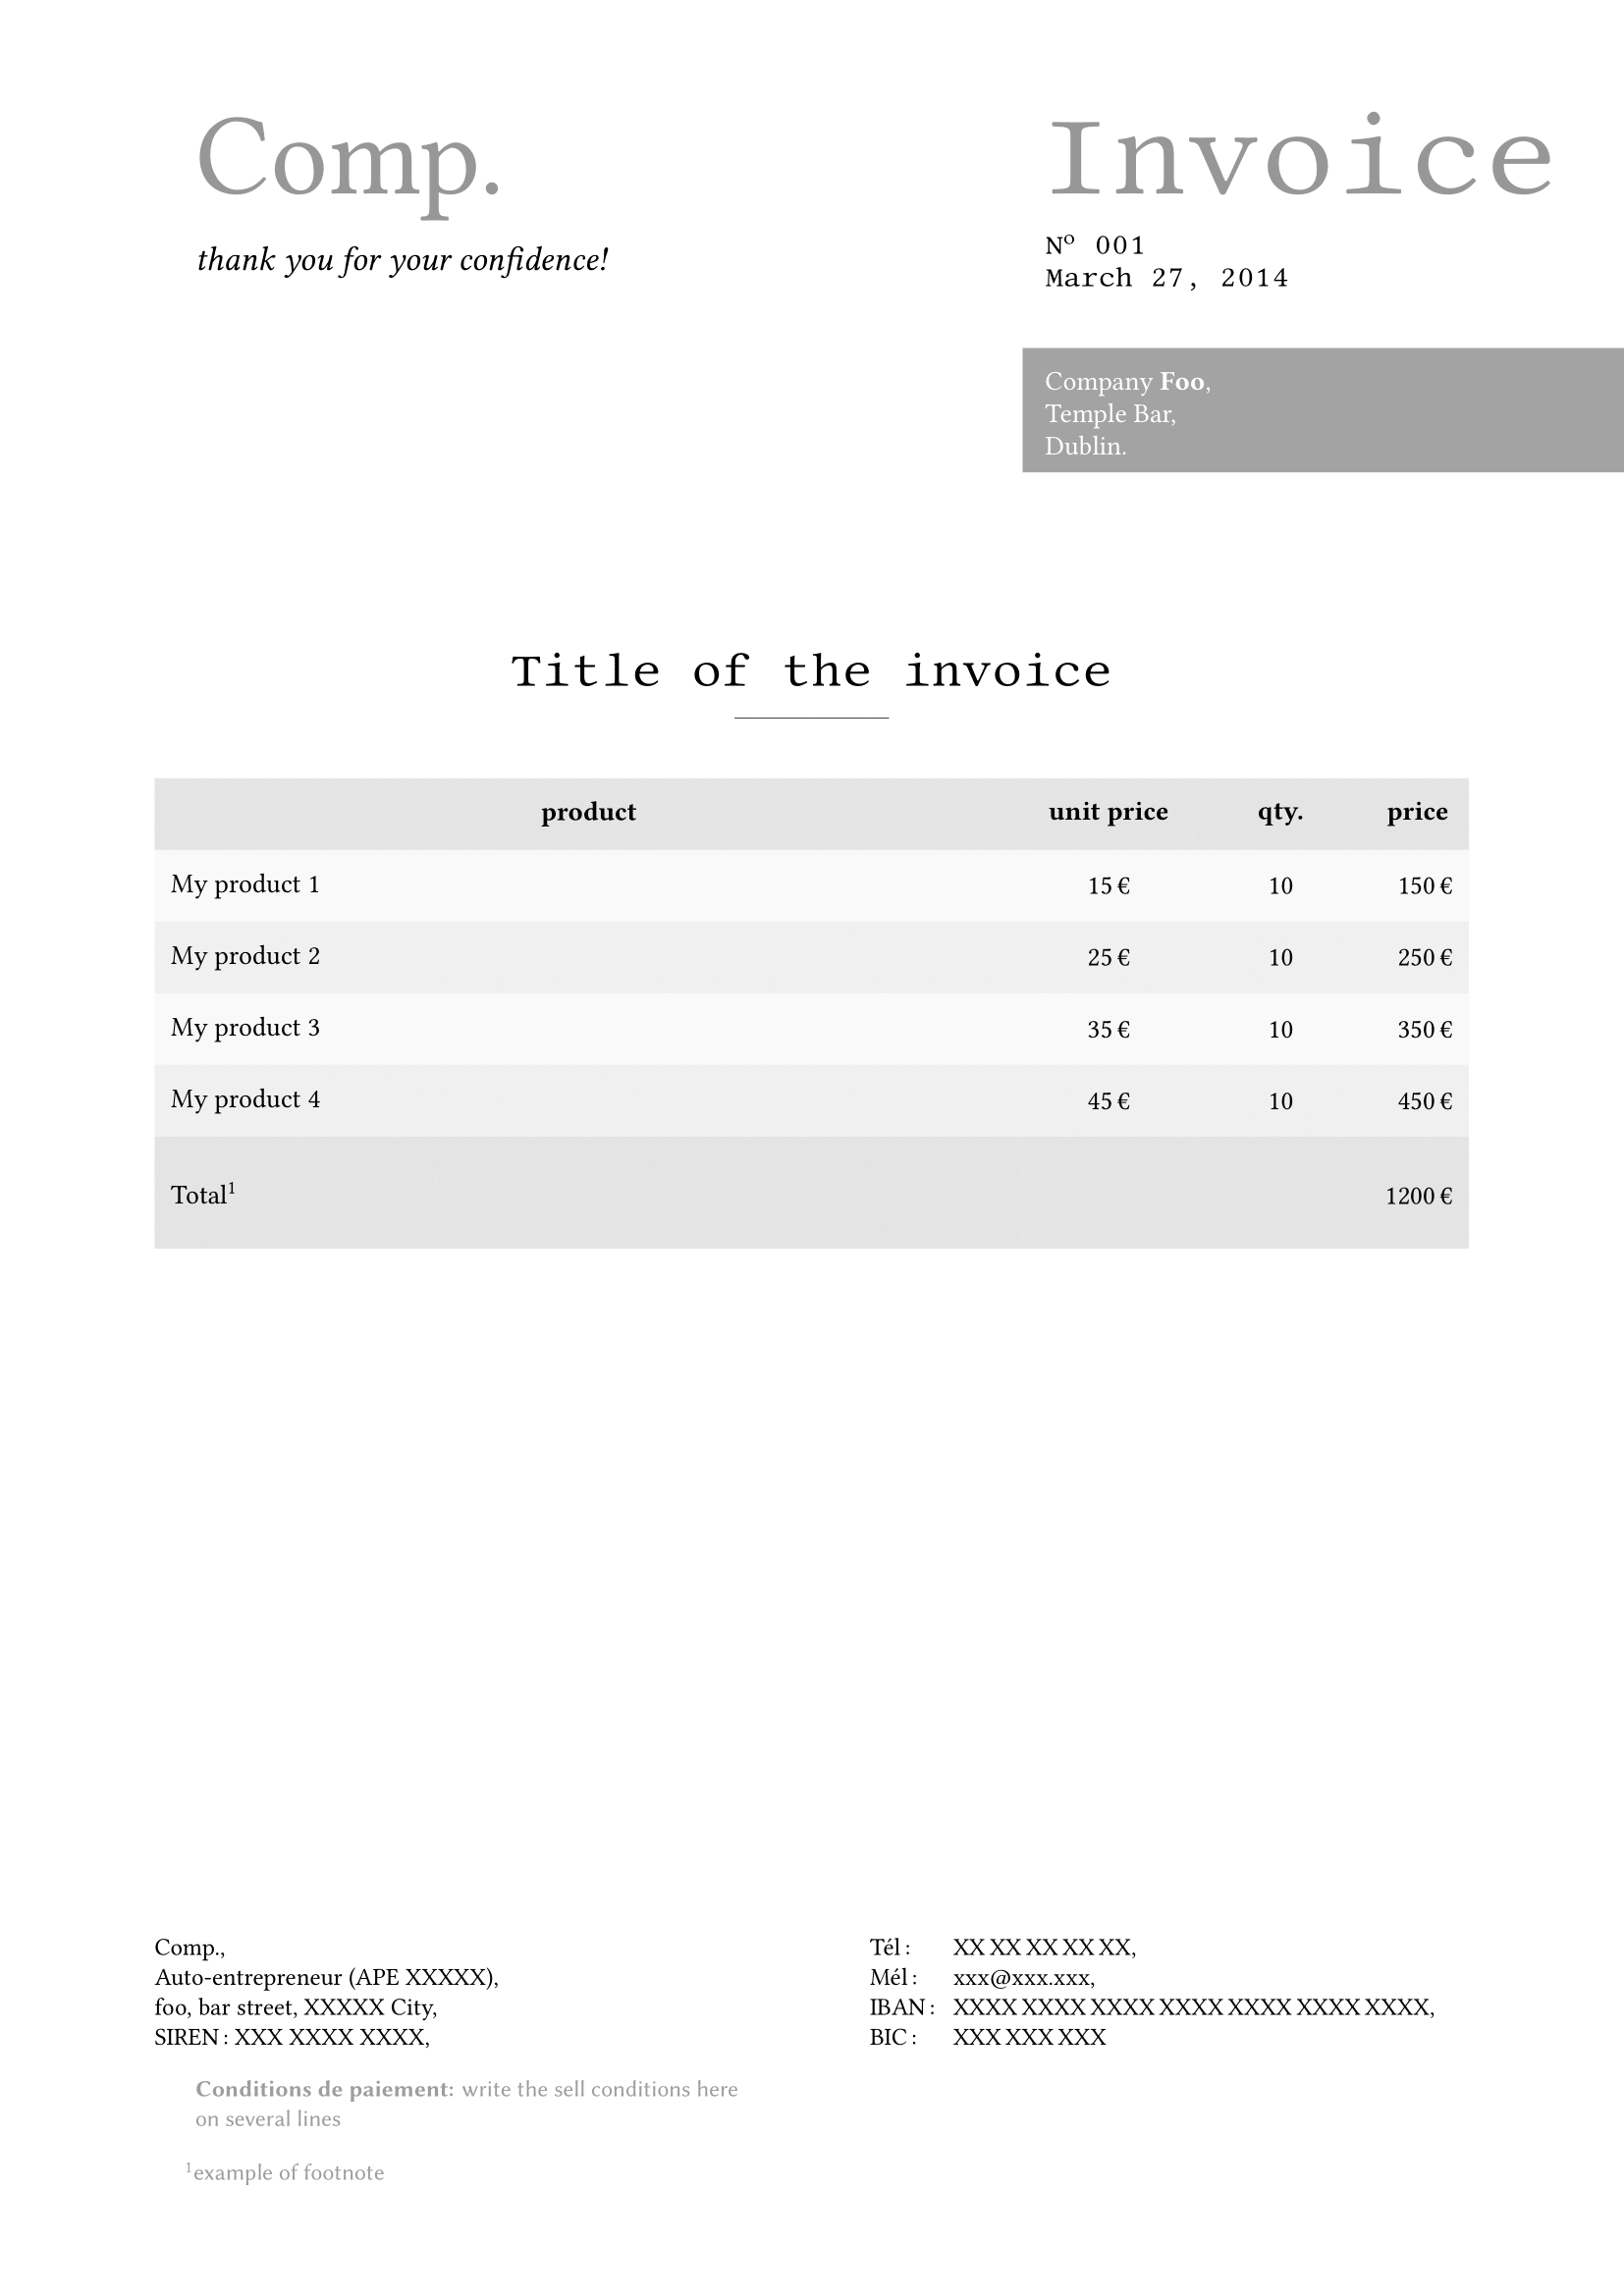
\includegraphics[width=1.85in,height=\textheight]{images/chapitre5_TStemp.png}

}

\caption{\label{fig-invoice}Exemple de gabarit LaTeX de feuille de temps
newline \emph{Source}~: Roux (2013).}

\end{figure}%

Les Figure~\ref{fig-cv} et Figure~\ref{fig-invoice} ne sont que quelques
exemples des milliers de gabarits de documents LaTeX disponible en
ligne. Plusieurs d'entre eux peuvent être téléchargés à partir du site
Web d'(Modèles, 2023). Vous pouvez y naviguer et voir quel gabarit
convient le mieux à vos besoins. Certaines manières plutôt spécifiques
de formater le texte sont présentement disponibles avec LaTeX ou
Markdown bien que non disponibles en Word, ce qui constitue une autre
preuve de leur grande \emph{flexibilité} et capacité de
\emph{personnalisation}. Bien qu'il soit rare que nous ayons absolument
besoin de personnaliser le texte ainsi, ces possibilités peuvent
s'avérer utiles lorsque vous rédigez un texte qui doit se conformer en
tout point à un gabarit spécifique. En effet, certaines revues
scientifiques, maisons d'édition et universités, dans le cadre de la
rédaction d'articles, de mémoires et de thèses par exemple, imposent ce
type de gabarit inflexible et parfois plutôt capricieux.

\subsubsection{Compatibilité entre types de
documents}\label{compatibilituxe9-entre-types-de-documents}

Un autre avantage non négligeable de Markdown --- qui le distingue à cet
égard de LaTeX --- est la \emph{flexibilité} des formats de documents
qui peuvent être produits. En effet, Pandoc Markdown, une extension du
langage Markdown de base, permet d'intégrer dans un seul document
plusieurs langages de balisage différents tels que Markdown, LaTeX et
HTML. Quarto utilise Pandoc Markdown et est également habilité à
travailler avec des extraits de code \texttt{R} ou Python. Ceci permet
donc à l'utilisateur ou à l'utilisatrice de bénéficier des
fonctionnalités de différents langages dans un seul document, rendant
ainsi possible une variété de \emph{personnalisations} qui ne seraient
pas possibles autrement. Qui plus est, puisque Markdown permet de créer
des fichiers Word réguliers, PDF professionnels et HTML à partir d'un
même document, vous pouvez choisir à votre convenance et à tout moment
de quelle manière sera compilé le document rédigé. Cette possibilité de
créer des documents Word est particulièrement pratique dans le cadre de
collaboration avec des chercheuses et chercheurs n'utilisant pas les
langages de balisage ainsi que lors de l'envoi de manuscrits à des
revues scientifiques, puisque certaines d'entre elles exigent de
recevoir ceux-ci sous forme de document Word.

\subsubsection{Popularité}\label{popularituxe9}

La popularité de certains langages de balisage dans le monde de la
recherche confère un avantage considérable à celles et ceux qui savent
les utiliser. La maîtrise de ces langages offre aux chercheurs et
chercheuses une polyvalence lorsqu'ils doivent collaborer avec diverses
équipes de recherche utilisant différentes méthodes de travail. Par
exemple, depuis sa création LaTeX a été adopté largement par le milieu
de la publication de travaux scientifiques (Gaudeul, 2007). À titre
indicatif, le logiciel Overleaf était utilisé en 2022 par 11 millions
d'utilisateurs et utilisatrices dans 189 pays autour du globe. Plus de
2000 compagnies et 6800 universités utilisent Overleaf pour écrire en
LaTeX (\emph{Wow! {Ten} Million Users!}, s.~d.). La popularité des
langages de balisages en fait donc un outil difficile à contourner pour
une personne qui voudrait poursuivre une carrière en recherche
académique. L'avantage ci-bas sur la gestion des embûches illustre
également comment la popularité permet une meilleure gestion de
celles-ci.

\subsubsection{Gestion des embuches}\label{gestion-des-embuches}

Bien que l'apprentissage de LaTeX et de Markdown puisse être parsemé de
nombreuses embuches, ces deux langages bénéficient d'une communauté
d'utilisateurs et d'utilisatrices en ligne sur laquelle il est possible
de s'appuyer afin de résoudre tout problème rencontré. Ces individus ---
particulièrement les plus expérimentés --- sont nombreux à partager leur
expérience à leurs collègues rencontrant des problèmes afin de
contribuer à régler ceux-ci. Cette communauté est présente sur une
multitude de sites Web, bien que le point de rencontre principal soit le
forum (\textbf{stackoverflowStackOverflow2023?}), qui est également
utilisé pour régler des problèmes de programmation et est abordé plus en
détail dans le chapitre 4. Une simple recherche sur Google d'un problème
rencontré avec LaTeX ou Markdown vous offrira des liens vers des
échanges pertinents ayant eu lieu sur Stack Overflow ou encore vers de
la documentation technique. Vous pourrez donc filtrer les résultats et
observer les nombreuses solutions envisageables à votre problème afin de
définir laquelle est la plus appropriée dans votre situation. Il est
important de noter, toutefois, que cette communauté est nettement plus
développée pour les utilisateurs de LaTeX que de Markdown, puisque ce
dernier langage est moins répandu que le premier.

Également, avec l'émergence de l'intelligence artificielle (IA), de
nombreux modèles d'IA génératifs commencent à émerger comme des
ressources d'aides utiles pour les chercheuses et les chercheurs. Au
moment de la rédaction du présent chapitre, le \emph{chatbot} ChatGPT,
développé par OpenAI et basé sur le grand modèle de langage (\emph{large
language model}, LLM) GPT-3.5, est une ressource d'aide en émergence en
ce qui a trait aux langages de balisage. Le corpus de données sur lequel
il a été formé inclut une grande variété de langages et de styles
d'écriture, incluant LaTeX et Markdown. Ainsi, il est possible de poser
des questions en langage courant à ce \emph{chatbot} lorsque des
problèmes de balisage sont rencontrés. Celui-ci fournira en réponse le
texte avec les balises adéquates pour régler le problème. Cela
s'applique même pour des problèmes pour lesquels la réponse n'est pas
directement indiquée sur Stack Overflow, lorsque la logique des langages
est comprise par ces modèles basés sur l'IA. ChatGPT est toutefois plus
outillé en LaTeX qu'en Markdown ou en Quarto en raison de la plus grande
abondance de ressources en LaTeX disponibles en ligne, bien que ses
capacités soient en constante amélioration. Il arrive cependant
régulièrement que les réponses des modèles de langage comme ChatGPT soit
erronées --- tout comme certaines réponses sur Stack Overflow peuvent ne
pas être adaptées à régler un problème similaire vécu sur un autre
ordinateur, avec des paramètres différents. Il demeure donc important de
vérifier les réponses des modèles basés sur l'IA afin de ne pas avoir de
mauvaises surprises lors de la compilation du code. Ainsi, il est utile
de s'appuyer autant sur la communauté d'utilisatrices et d'utilisateurs
de langages de balisage qui échange des ressources en ligne que sur les
modèles de langage basés sur l'IA.

\subsubsection{Philosophie du code source ouvert et du logiciel
libre}\label{philosophie-du-code-source-ouvert-et-du-logiciel-libre}

L'utilisation des langages de balisage s'inscrit bien dans la
philosophie du logiciel libre. Le langage LaTeX est distribué sous la
license \emph{LaTeX project public license} (LPPL), alors que Quarto 1.4
est distribué sous la license du Massachusetts Institute of Technology
(MIT). Moyennant le respect de leurs licenses respectives, ces licenses
permettent ainsi aux utilisateurs de LaTeX et de Quarto d'utiliser ces
langages comme ils le souhaitent, de redistribuer des copies, de
modifier le fonctionnement de ces langages et d'en redistribuer des
versions améliorées. Bien que LaTeX et Quarto ne soient pas des
logiciels, leur license utilisation est cohérente avec la philosophie du
logiciel libre et permet à ces langages d'être utilisés dans de nombreux
logiciels.

D'autre part, LaTeX et Quarto sont deux langages à code source ouvert
(\emph{open source}). Ainsi, leur distribution est entièrement gratuite,
il n'y a rien à payer. Leur code source est disponible et les
changements à ce code doivent être indiqués. Les licences LPPL et MIT ne
discriminent pas certains groupes ou personnes, et elles ne restreignent
personne dans l'utilisation pour un domaine d'activité. Ces deux
licences ne sont pas spécifiques pour un produit, ce qui signifie que
ces deux langages peuvent être utilisés dans plusieurs logiciels et
programmes. Elles sont également technologiquement neutres, rendant
ainsi LaTeX et Quarto accessibles aux utilisateurs de tous les systèmes
d'exploitation.

\subsection{Inconvénients}\label{inconvuxe9nients-1}

Il existe toutefois des désavantages inhérents à l'utilisation des
langages de balisage. L'un des principaux désavantages de Markdown et de
LaTeX est le fait qu'ils ne comportent aucun système de suivi des
modifications lors de travaux collaboratifs. Pour réviser un travail
fait en langage de balisage, des commentaires peuvent être ajoutés sur
le fichier sortant --- nécessairement PDF pour un fichier sortant
produit avec LaTeX. Des commentaires peuvent aussi être faits
directement dans le document LaTeX ou Markdown, à l'aide de balises
spécifiques. Ces commentaires n'apparaissent cependant pas dans le
fichier sortant. Le suivi des modifications en LaTeX et Markdown
nécessite donc souvent l'utilisation de Git et de GitHub, qui sont
abordés plus en détail dans le chapitre 8. Même avec une plateforme de
gestion des versions comme GitHub, les longs paragraphes ayant fait
l'objet de plusieurs modifications peuvent être longs à comparer par
rapport aux logiciels de traitement de texte, qui permettent de
visualiser les propositions d'ajouts et de retraits de caractères de
manière plus intuitive. Le suivi des modifications en logiciel de
traitement de texte permet également de distinguer les auteurs de
différents commentaires par leurs noms, alors que les ajouts et retraits
itératifs en GitHub peuvent rendre difficile l'identification de
l'auteur d'une modification. Pour ces raisons, et aussi pour faciliter
la mise en page par les éditeurs, certaines revues scientifiques
refusent les fichiers PDF et demandent que les soumissions soient faites
en format DOCX --- ce qui pose problème pour les utilisateurs de LaTeX
mais pas ceux de Markdown.

Les langages de balisage comportent également un autre désavantage
important dans certains cas~: l'absence d'un correcteur de fautes de
français complet, en particulier pour corriger les fautes autres que
celles d'orthographe en français. Parmi les principaux endroits
permettant l'édition en langages de balisage, Visual Studio Code (VS
Code) et Overleaf comprennent tous deux une extension LanguageTool (LTeX
pour pour VS Code), qui permet la révision orthographique et syntaxique
dans plusieurs langues. VS Code possède également une extension Antidote
pour les personnes qui paient déjà pour ce logiciel. D'autres extensions
linguistiques existent également pour VS Code, de même que pour les
logiciels de traitement de texte comme Word. Cependant, RStudio ne
possède qu'un correcteur \emph{orthographique} de base, disponible en
plusieurs langues. Ce correcteur ne repère pas les erreurs de syntaxe,
de grammaire ou de forme, entre autres. Ces éléments sont pourtant
essentiels pour la rédaction de textes académiques\footnote{Pour les
  utilisateurs de RStudio, il est souvent nécessaire de modifier le
  texte dans un logiciel de traitement de texte externe pour faire une
  révision linguistique complète, puis d'intégrer les corrections en
  collant le texte corrigé dans le document original en Markdown ou
  LaTeX. Une application de bureau Grammarly peut également être
  intégrée sur RStudio. Cette application repère les erreurs de syntaxe,
  mais ne corrige que l'anglais, et certains soucis de repérage des mots
  aux bons endroits dans le texte en rendent présentement l'utilisation
  difficile.}, d'autant plus que les utilisateurs de LaTeX ont tendance
à faire davantage de fautes d'ortographe et de grammaire lors de la
rédaction que les utilisateurs de Word (Knauff \& Nejasmic, 2014). Nous
décourageons ainsi l'utilisation de RStudio pour l'édition de fichiers
LaTeX et Quarto, et nous encourageons fortement les utilisateurs
d'Overleaf et de VS Code d'utiliser des extensions permettant la
correction grammaticale telles que LanguageTool/LTeX.

Enfin, les langages de balisage, contrairement aux logiciels de
traitement de texte, nécessitent d'être compilés, ce qui implique que
deux fichiers coexistent~: le fichier où le langage de balisage est
utilisé --- format \texttt{.tex} pour LaTeX, \texttt{.md} pour Markdown
ou encore \texttt{.qmd} pour Quarto --- ainsi que le fichier où le texte
final balisé apparait --- généralement \texttt{.pdf}, \texttt{.docx} ou
\texttt{.html}. La compilation peut prendre un temps variable selon la
complexité du document, mais dure typiquement une quinzaine de secondes.
Le fait de devoir travailler avec deux fichiers en parallèle et de ne
pas voir immédiatement l'effet des balises sur le document final
constitue ainsi un autre désavantage des langages de balisage.

LaTeX comporte aussi quelques difficultés techniques particulières qui
peuvent être réglées ou diminuées en travaillent en Markdown.
Premièrement, LaTeX est difficile à apprendre. Certaines tâches qui
peuvent sembler simples comme l'ajout d'un tableau peuvent nécessiter de
nombreuses lignes de code. De plus, à la moindre erreur de frappe dans
l'utilisation d'une balise, le code risque de ne pas fonctionner et de
ne pas produire le document PDF souhaité. C'est ce qu'on appelle une
erreur de compilation. Markdown est un langage plus simple à apprendre,
avec des balises plus courtes et intuitives. Il occasionne donc moins
d'erreurs de compilation.

Deuxièmement, LaTeX est peu compatible avec les logiciels de traitement
de texte comme Word. Pour transférer un fichier créé à partir d'un
logiciel de traitement de texte vers LaTeX, les balises doivent être
ajoutées manuellement une par une. À l'inverse, pour transférer un
document LaTeX vers un fichier de traitement de texte, le convertisseur
Pandoc peut être utilisé, mais celui-ci ne repère pas toutes les balises
et il est souvent nécessaire de faire des aller-retour entre le fichier
LaTeX original et le fichier converti en format DOCX pour s'assurer du
succès de la conversion. Parfois, les balises doivent être retirées une
par une et le formatage doit être refait en utilisant les boutons
fournis sur le logiciel de traitement de texte. Il est aussi possible de
copier le texte directement à partir du fichier PDF produit par LaTeX
vers un logiciel de traitement de texte, mais les fins de ligne sont
interprétées par Word, Pages ou Writer comme des retours plutôt que des
espaces, et les accents sont souvent mal copiés et doivent être réécrits
manuellement. Encore une fois, Markdown évite ce problème en permettant
d'écrire un fichier DOCX à partir du langage de balisage. Le formatage
du fichier DOCX demeure un peu compliqué cependant et doit être fait à
partir du modèle d'un autre document DOCX formaté tel que souhaité. De
plus, les fichiers DOCX ne peuvent pas être transformés en format
Markdown. Quarto permet d'écrire un texte en format Markdown et de
produire un fichier DOCX à partir d'un gabarit Word. De plus, pour les
fichiers Word à transformer en format Markdown, les balises plus simples
en Markdown qu'en LaTeX rendent la tâche plus simple.

Somme toute, Word n'est pas à antagoniser et demeure très utile pour des
tâches simples. Cependant, dans le monde académique, la production de
fichiers de qualité faisant appel à des graphiques, tableaux et blocs de
code personnalisés de qualité et automatisés est simplifiée en utilisant
des langages de balisage. Il n'est ainsi pas anodin que ces langages
soient adoptés largement dans le monde académique. Pour ces raisons, il
est avantageux pour une personne poursuivant une maitrise en science
sociale ou autre de passer outre la difficulté initiale d'apprentissage
des langages de balisage. L'apprentissage de ces langages permettra de
s'aligner sur les pratiques répandues dans le milieu académique et
d'améliorer davantage la qualité de la production d'écrits
scientifiques.

\section{Conclusion: Pièges et
astuces}\label{conclusion-piuxe8ges-et-astuces}

Maintenant que vous avez une meilleure idée de ce que sont les langages
de balisage et de leur utilité, la prochaine étape consiste à
expérimenter par vous-même. Le chapitre se termine donc par un résumé
des étapes à suivre pour devenir expert dans les langages de balisage.

La première étape consiste à commencer à expérimenter dès que possible,
sans se laisser freiner par l'incompréhension. Il n'est pas nécessaire
de tout comprendre des langages de balisage pour produire un document de
qualité. Avec cet état d'esprit, vous franchirez les difficultés
initiales de la l'apprentissage des langages de balisage plus
rapidement.

Ensuite, ne pas hésiter à utiliser les ressources disponibles pour
gagner du temps. Les ``cheat sheets'' disponibles en ligne, l'aide de
LLMs (Large Language Models) qui connaissent les langages de balisage
(par exemple, ChatGPT), et le recours à des sites comme Stack Overflow
peuvent être très utiles. Si on ne fait pas appel à des ressources
externes, il peut devenir facile de devenir fâché contre soi-même ou
contre l'infrastructure informatique. Il est parfaitement normal de
demander de l'aide externe, même pour un expert.

La troisième étape est de ne surtout pas sous-estimer l'aide de ses
pairs. N'hésitez pas à poser des questions et à demander de l'aide à des
personnes plus expérimentées pour résoudre des problèmes que vous ne
parvenez pas à résoudre avec les ressources externes.

Avant d'aborder la quatrième et dernière étape, il est important de
mentionner quelques pièges à éviter lors de la transition de débutant à
expert. Tout d'abord, faites attention aux exigences des revues lorsque
vous soumettez des articles scientifiques. Certaines demandent des
articles au format Word tandis que d'autres préfèrent les langages de
balisage. Savoir comment convertir correctement les documents est donc
un atout.

De plus, ne vous limitez pas à un seul langage de balisage et soyez
polyvalent, car travailler en collaboration peut nécessiter de s'adapter
aux pratiques des partenaires. Veillez également à éviter les erreurs
lors de la compilation des documents écrits en langage de balisage en
portant une attention particulière aux balises et en ne les laissant pas
s'accumuler. Une bonne façon de veillez à ce que les erreurs ne
s'accumulent pas est de compiler fréquemment vos documents en cours de
production.

Un des pièges qui peut sembler évident mais qui mérite d'être répété est
de faire attention à la qualité de la langue écrite. Soyez ainsi à
l'affut de la présence de correcteur automatique ou non dans vos
environnements d'édition. Vérifiez aussi si ce correcteur automatique
est dans la bonne langue (français canadien, anglais canadien, etc.).

Enfin, évitez les conflits Git lors de la collaboration sur GitHub en
coordonnant efficacement les travaux d'équipe et en utilisant Git de
manière optimale pour tirer parti des langages de balisage. Il est donc
important de se renseigner quant aux bonnes pratiques à suivre afin de
collaborer efficacement avec Git. À cet égard, beaucoup de ressources
sont à votre disposition en ligne.

Pour conclure, la dernière étape pour devenir expert en langages de
balisage est d'être créatif. Explorez les différentes balises et
utilisez-les de manière inventive. Les langages de balisage vous
permettront d'effectuer des tâches que vous n'auriez pas pu réaliser
facilement en utilisant un logiciel de traitement de texte classique.
Ils vous permettront de produire des documents professionnels dans
différents formats personnalisés, produits avec des processus
automatisés, avec une grande qualité graphique.

\begin{table}
\centering
\begin{talltblr}[         %% tabularray outer open
caption={Résumé des critères de sélection - Langages de balisage},
entry=none,label=none,
note{a}={Bien que LaTeX offre une bonne transparence et réplicabilité, son utilisation via Overleaf peut être limitée sans version payante, notamment pour l'intégration avec GitHub et Dropbox. Ces limitations ne s'appliquent pas à des environnements comme RStudio ou VS Code.},
note{b}={Quarto est relativement récent et semble prendre de plus en plus la place de R Markdown parmis la communauté d'utilisateurs de R. Le nombre d'utilisateurs de Quarto est donc appelé à croitre dans les prochaines années.},
]                     %% tabularray outer close
{                     %% tabularray inner open
width={0.75\linewidth},
colspec={X[]X[]X[]X[]},
}                     %% tabularray inner close
\toprule
Critères & LaTeX & R Markdown & Quarto \\ \midrule %% TinyTableHeader
Accessibilité (Gratuit ou peu dispendieux) & Oui         & Oui    & Oui     \\
Existence d'une communauté d'utilisateurs  & Très grande & Grande & Moyenne\textsuperscript{b} \\
Popularité dans le champ                   & Oui         & Oui    & Oui     \\
Compatibilité avec d'autres outils         & Moyenne     & Forte  & Forte   \\
Transparence et réplicabilité              & Oui        \textsuperscript{a} & Oui    & Oui     \\
Adaptabilité et flexibilité                & Très forte  & Forte  & Forte   \\
\bottomrule
\end{talltblr}
\end{table}

\section{Références}\label{ruxe9fuxe9rences}

\bookmarksetup{startatroot}

\chapter{Outils d'intelligence
artificielle}\label{outils-dintelligence-artificielle}

\begin{center}

Jozef Rivest, Laurence-Olivier Foisy, Hubert Cadieux

\end{center}

Ce chapitre vise à initier les lecteurs à ce qu'est l'intelligence
artificielle (IA), aux enjeux qu'elle engendre ainsi qu'à son potentiel
pour les sciences sociales. Nous souhaitons d'abord et avant tout mener
les lecteurs vers la réflexion. Dans ces pages, il y a beaucoup plus de
questions que de réponses. Cet état de fait reflète bien l'état de la
connaissance que nous avons sur l'IA. Nous sommes aussi bien loin d'être
des spécialistes en la matière. Malgré cela, nous pensons qu'initier la
réflexion et la discussion s'impose. Se poser des questions et tenter de
trouver des réponses ne peut que générer des bénéfices. Par conséquent,
si ce chapitre aura permis d'éclairer certains enjeux, ou s'il stimulera
davantage de questionnement, alors nous aurons réussi notre objectif.

Nous débutons par définir et expliquer ce qu'est l'intelligence
artificielle. Bien que ça ne soit pas une tâche facile, nous souhaitons
simplement donner une idée générale de ce qu'il s'agit. Ensuite, nous
souhaitons mettre l'accent sur l'évolution constante de ce champ de
recherche, ainsi que les défis que ça pose. La section suivante se
penche sur certains enjeux éthiques lié à l'utilisation de l'IA,
notamment en ce qui concerne le plagiat. Cela nous mène à se questionner
sur la place du chercheur, aujourd'hui et dans le futur, avec l'arrivé
de ces nouvelles technologies. La dernière section se penchera sur la
place de cette technologie en sciences sociales. Quel usage pourrait-on
en faire, et surtout quels en sont les limites.

\section{Définition et différents type
d'IA}\label{duxe9finition-et-diffuxe9rents-type-dia}

Qu'est-ce que l'intelligence artificielle (IA)? Est-ce quelque chose
d'homogène, ou s'agit-il plutôt « des intelligences artificielles »?
Dans un premier temps, il est important de préciser que l'intelligence
artificielle est un champ d'études (Devedzic, 2022). Par conséquent, il
s'agit d'un ensemble d'objets, relativement vaste et en constante
expansion, qui s'intéressent, à sa façon, à l'intelligence artificielle.
Pour préciser ce propos, prenons l'exemple de la science politique.
Malgré la formulation au singulier, la science politique est un grand
ensemble de différents sous-champs d'études, qui ont chacun leur propre
objet d'intérêt. La philosophie politique, les relations
internationales, la politique comparée et l'étude de l'opinion publique,
par exemple, sont tous des sous-champs qui s'intéressent, à leur façon,
au phénomène politique. Dans le même sens, et compte tenu de cette
pluralité de perspectives, il est important de noter qu'il n'y a pas de
consensus dans la définition de l'IA (Wang, 2019 ; König et al., 2022).
De plus, la rapidité du développement de ce champ rend le traçage de
frontières définitionnelles plutôt difficile : comment définir, d'une
manière précise et consensuelle, quelque chose qui évolue constamment
(Devedzic, 2022 ; Bertolini, 2020, pp.~15)?

Deux définitions de l'IA peuvent tout de même être retenues. La première
vient de John McCarthy (2007, pp.~2) : « Il s'agit de la science et de
l'ingénierie qui consistent à créer des machines
intelligentes\footnote{Intelligence étant définit de la façon suivante :
  « L'intelligence est la partie informatique de la capacité à atteindre
  des objectifs dans le monde. On trouve différents types et degrés
  d'intelligence chez l'homme, chez de nombreux animaux et chez
  certaines machines. » (McCarthy, 2007, pp.~2)}, en particulier des
programmes informatiques intelligents. Elle est liée à la tâche
similaire consistant à utiliser des ordinateurs pour comprendre
l'intelligence humaine, mais l'IA ne doit pas se limiter aux méthodes
qui sont biologiquement observables. » {[}Traduction DeepL{]} La seconde
définition provient de la compagnie IBM (2023a) : « Dans sa forme la
plus simple, l'intelligence artificielle est un domaine qui combine
l'informatique et des ensembles de données robustes pour permettre la
résolution de problèmes. Elle englobe également les sous-domaines de
l'apprentissage automatique et de l'apprentissage profond, qui sont
souvent mentionnés en conjonction avec l'intelligence artificielle. Ces
disciplines sont composées d'algorithmes d'IA qui cherchent à créer des
systèmes experts qui font des prédictions ou des classifications basées
sur des données d'entrée. » {[}Traduction DeepL{]} Ces extraits
permettent de comprendre que l'IA consiste à reproduire artificiellement
certaines capacités cognitives humaines, afin de rendre les machines «
intelligentes » en leur donnant la capacité de résoudre des problèmes
par elles-mêmes.

Ces définitions restent toutefois à préciser, notamment dans le champ
d'application de l'IA : qu'en est-il concrètement ? Comment est-ce
utilisé ? Comment ça fonctionne ? Si l'IA se distingue enn plusieurs
types, en faire la liste et identifier leurs différentes branches et
applications possibles serait fastidieux et s'écarterait de l'objectif
de ce chapitre introductif. Cependant, pour ceux désirant en savoir plus
sur le sujet, les articles de McCarthy (2007) et de Hanchen et al.
(2023), ainsi que le Cambridge Handbook of Artificial Intelligence
(König et al., 2022) sont très riches et illustratifs sur ce qu'est l'IA
ainsi que sur ses champs d'applications.

Avant toute chose, il est important de distinguer l'IA général (strong)
du précis (narrow). Le premier, et le moins populaire en nombre de
recherches et d'applications, cherche à développer une machine qui
aurait les mêmes capacités cognitives que l'humain, non seulement en
termes de résolution de problème, d'apprentissage et de planification,
mais aussi qui serait dotée d'une conscience de soi (IBM, 2023a ; König
et al., 2022). Le deuxième est plus restrictif, se limitant à la
réalisation d'un ou de plusieurs objectifs spécifiques. De ces deux
visées, il y a trois principaux champs de recherche qui se penchent sur
les méthodes de fonctionnement de l'IA : l'apprentissage machine
(machine learning), les réseaux neuronaux artificiel (artificial neural
networks) ainsi que l'apprentissage profond (deep learning).

L'apprentissage machine : « {[}\ldots{]} consiste à programmer des
ordinateurs pour optimiser un critère de performance à l'aide de données
d'exemple ou d'expériences passées. Nous avons un modèle défini jusqu'à
certains paramètres, et l'apprentissage est l'exécution d'un programme
informatique pour optimiser les paramètres du modèle à l'aide des
données d'entraînement ou de l'expérience passée. » {[}Traduction
DeepL{]} (Alpaydin et Bach 2014, 3). Le but est d'entraîner le modèle
afin qu'il puisse reconnaître des tendances, et qu'il puisse décrire
et/ou faire des prédictions à partir de ces tendances (Alpaydin \& Bach,
2014, pp.~3). Il est le champ le plus populaire dans la recherche faite
sur l'IA, notamment parce qu'il constitue une base importante pour les
autres recherches dans le domaine (Devedzic, 2022).

Ensuite, un sous-champ de l'apprentissage machine, l'apprentissage
profond : « {[}\ldots{]} fait référence à un réseau neuronal composé de
plus de trois couches {[}\ldots{]}. L'apprentissage en profondeur
automatise une grande partie de l'extraction des caractéristiques,
éliminant ainsi une partie de l'intervention humaine manuelle nécessaire
et permettant l'utilisation d'ensembles de données plus importants. Il
peut ingérer des données non structurées dans leur forme brute et
déterminer automatiquement la hiérarchie des caractéristiques qui
distinguent les différentes catégories de données les unes des autres,
ne nécessitant pas d'intervention humaine. » {[}Traduction DeepL{]}
(IBM, 2023a). Ainsi, l'apprentissage profond permet une certaine forme
d'automatisation des tâches demandées à l'IA, en lui fournissant les
capacités nécessaires d'apprendre par lui-même pour corriger et
améliorer son fonctionnement. Pour ce faire, on doit développer des
structures neuronales artificielles, qui s'inspirent des neurones du
cerveau humain.

C'est d'ailleurs la tâche de ceux qui s'intéressent aux réseaux
neuronaux artificiels : « Les réseaux neuronaux artificiels (RNA) sont
constitués d'une couche de nœuds, contenant une couche d'entrée, une ou
plusieurs couches cachées et une couche de sortie. Chaque nœud, ou
neurone artificiel, se connecte à un autre et possède un poids et un
seuil associés. Si la sortie d'un nœud individuel est supérieure à la
valeur seuil spécifiée, ce nœud est activé et envoie des données à la
couche suivante du réseau. Dans le cas contraire, aucune donnée n'est
transmise à la couche suivante du réseau. » {[}Traduction DeepL{]} (IBM
2023b). Ainsi, le but est de reproduire les structures cognitives
humaines, afin de permettre à l'IA d'accomplir des tâches plus
complexes. L'une des principales utilités de ce sous-champ est qu'il
permet d'augmenter la rapidité du classement de données ; la
reconnaissance vocale ou d'image, par exemple, ne prend que quelques
minutes grâce à cela, contrairement à plusieurs heures lorsque fait par
des humains (IBM, 2023b).

\section{L'évolution constante de
l'IA}\label{luxe9volution-constante-de-lia}

Plusieurs chercheurs, dont le professeur Yoshua Bengio de l'Université
de Montréal, ont lancé plusieurs avertissements sur le développement de
l'IA, notamment à cause de la rapidité de son évolution. Dans un article
paru dans The Economist, M. Bengio (2023) nous dit qu'il prévoyait le
développement d'une IA avec des capacités similaires à celles de
l'humain d'ici quelques décennies, peut-être un siècle. Depuis l'arrivée
de ChatGPT-4, celui-ci a revu sa prédiction pour la situer entre
quelques années et quelques décennies (Bengio, 2023). Dans les dix
dernières années seulement, les systèmes de reconnaissance d'images et
de langages en sont venus à dépasser les capacités humaines (Roser,
2022). La figure 1 présente cette évolution.

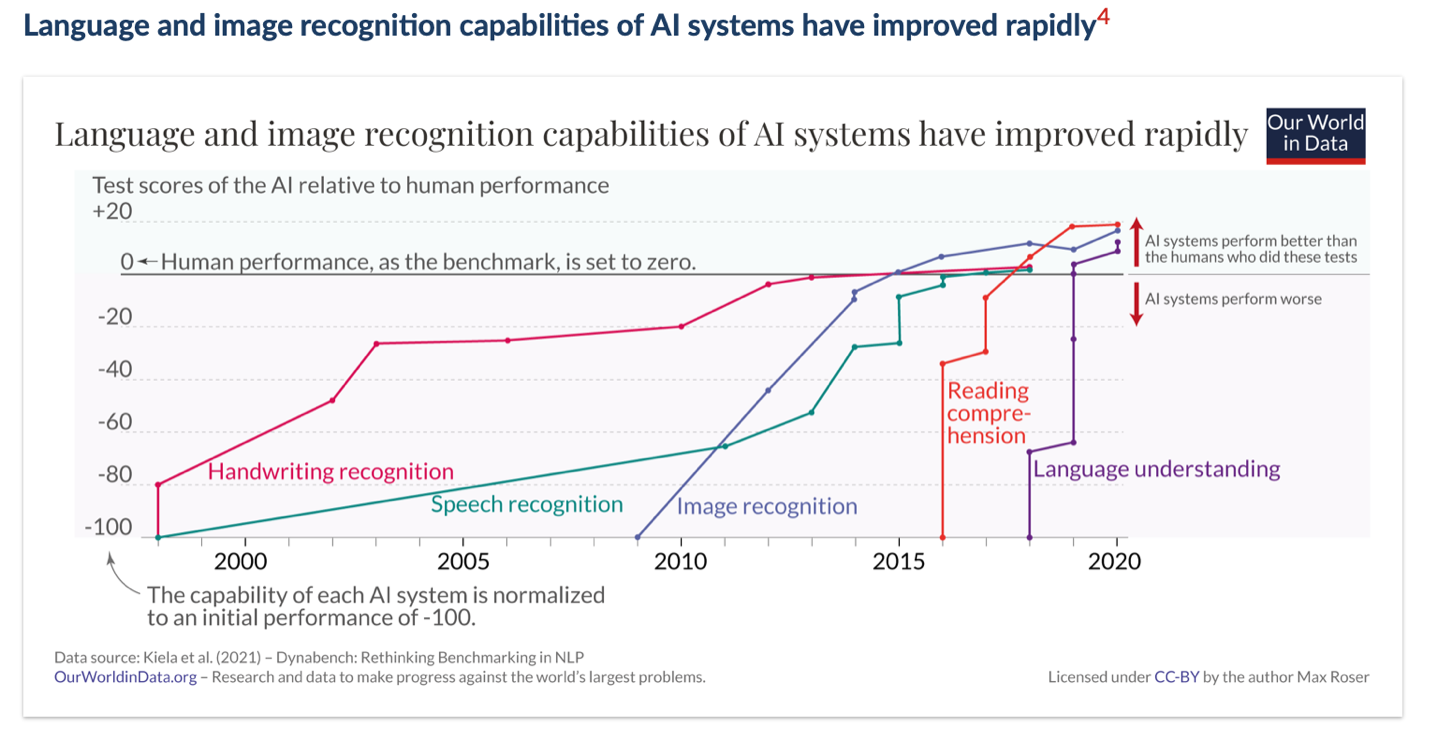
\includegraphics{images/chapitre9_figure1.png} \newpage{}

Comme on le remarque, cette évolution ne suit pas une trajectoire
linéaire. Depuis 2015, la plupart de ces technologies ont évolué de
manière quasi-exponentielle. Cette progression fulgurante nous permet de
faire quelque constat pour appréhender l'évolution future. Ce qui est
intéressant de la recherche dans ce domaine, c'est que le développement
des capacités de l'IA permet, en retour, de la développer encore plus
rapidement. L'IA peut rendre l'IA exponentiellement plus puissante
(Harari, 2023). Elle est capable de se faire évoluer à une vitesse plus
grande, grâce à ses capacités de traitement de données et
d'auto-améliorassions, que si elle était uniquement dépendante de
l'humain.

En tant que chercheur en sciences sociales, pourquoi devrait-on être
préoccupé par le développement de l'IA? Tout d'abord, il est intéressant
de commencer à réfléchir ainsi qu'à analyser les différents impacts que
l'IA a sur nos sociétés. Les avancés dans le domaine en plus de
l'accessibilité à ces technologies, tel que Large Language Model (LLM),
en font de nouveaux objets d'étude actuel, et surtout sans grandes
réponses. Yuval Noah Harrari (2023), historien et philosophe, explique
dans un article que la capacité de l'IA à manipuler ainsi qu'à générer
du langage en font des outils puissants qui ont le potentiel d'avoir de
profond impact sur nos civilisations. Par conséquent, l'étude des effets
de l'IA sur nos sociétés devient un nouveau sujet de recherche dont tous
les champs des sciences sociales et sciences humaines ont intérêt à se
pencher. Présentement, il est anticipé que cette technologie puisse être
utilisée pour « générer et partager de fausses informations, érodant la
confiance sociale et la démocratie; pour surveiller, manipuler et
maîtriser les citoyens, nuisant aux libertés individuelles et
collectives; ou pour créer de puissantes armes physiques ou digitales
qui menaceraient la vie humaine. » {[}Traduction libre{]} (Bremmer \&
Suleyman, 2023, pp.~32). Compte tenu des conséquences potentielles que
ces technologies peuvent avoir sur le monde social, tous les domaines
scientifiques ont un fort incitatif à décloisonner leur savoir et leurs
analyses, en plus de maximiser l'interdisciplinarité et la recherche
collaborative. Une compréhension plus complète de ces changements ainsi
qu'une communication de ce savoir ne pourra que générer des bénéfices
pour le monde académique, social et politique.

\section{Les différents outils de
l'IA}\label{les-diffuxe9rents-outils-de-lia}

Cette section vise à présenter différents outils de l'intelligence
artificielle aux lecteurs. Ce qui est important de comprendre ici, et
pour faire suite à la section précédente, c'est que les outils présenté
ici risque d'avoir changé entre le moment d'écrire ce chapitre et le
moment où les lecteurs liront le chapitre. Certaines fonctionnalités
pourraient toujours être les mêmes, certaines pourraient avoir été
améliorées et d'autres pourraient être complètement nouvelles. Par
conséquent, l'objectif ici est de présenter certaines utilités et
fonctionnalités de l'IA, et surtout d'inciter les lectuers à développer
leurs propres capacités réflexives quant à leur utilisation de l'IA.
Cette technologie offre de nouvelles opportunités, mais elle apportea
aussi son lot d'enjeux et de questions dont il vaut mieux s'y intéresser
afin de développer une utilisation saine et intégre de ces outils.

Trois catégories d'outils seront présentées: les « \emph{Large Language
Models} » (LLM), les assistants de traduction ainsi que les assistants
de revue de littérautre.

\subsection{1. Les LLMs}\label{les-llms}

OpenAi (2019) définissent les grands modèles linguistiques (Large
language models ou LLMs en anglais) comme des modèles d'apprentissage
automatique de grande échelle, formés pour prédire le mot suivant dans
un texte en se basant sur les mots précédents. Ils sont entraînés sur de
vastes quantités de données textuelles, telles que des articles de
journaux, des livres, des pages web, des courriels, des messages de
médias sociaux, etc. Cette méthode d'entraînement simple permet aux
modèles de démontrer naturellement des compétences dans de nombreuses
tâches et domaines divers, sans nécessiter de formation spécifique à la
tâche. Il est important de noter que les GML ne sont que des algorithmes
de prédiction textuelle et ne possèdent pas la faculté de réfléchir ou
de comprendre.

L'intégration des grands modèles de langage (LLMs) via l'API d'OpenAI
dans la recherche en sciences sociales numériques ouvre des horizons
prometteurs pour l'analyse qualitative et quantitative des données
textuelles. L'utilisation de ces modèles en R permet aux chercheurs
d'exploiter des capacités avancées de traitement du langage naturel pour
une variété d'applications allant de la simple extraction de données à
des analyses complexes de contenu et de sentiment. Elle permet aussi de
générer des données pour l'analyse de biais algorithmiques en comparant
l'information générée par les modèles avec des données de référence
générées par des humains. Les LLMs peuvent être utilisés pour l'analyse
de sentiments, l'extraction d'entités et de relations, la génération de
résumés de texte, la simulation de dialogue, la traduction et la
localisation, et le développement d'outils personnalisés pour des
besoins spécifiques de recherche.

Voici quelques exmples d'utilisation des LLMs en sciences sociales:

Premièrement, les LLMs peuvent être utilisés pour l'analyse de
sentiments, permettant aux chercheurs de détecter des nuances dans les
opinions exprimées dans des corpus de données volumineux, tels que des
commentaires sur les réseaux sociaux, des critiques de produits, ou des
discours politiques. Cette analyse peut révéler des tendances de
sentiment général ou être segmentée pour examiner des variations entre
différents groupes démographiques ou chronologiques.

Deuxièmement, les LLMs offrent des capacités d'extraction d'entités et
de relation, ce qui est crucial pour structurer des données non
structurées comme des questions de sondage ouvertes. Les chercheurs
peuvent extraire des personnes, des lieux, des institutions, et même des
concepts ou des événements, liant ces entités à des thèmes spécifiques
ou à des contextes historiques et socio-politiques, enrichissant ainsi
les bases de données pour des études plus poussées.

Troisièmement, la génération automatique de résumés de textes par ces
modèles permet de condenser de grandes quantités d'informations en
résumés concis, facilitant l'analyse préliminaire de vastes archives de
textes, comme des articles de presse, des mémoires juridiques, ou des
écrits académiques. Cela aide les chercheurs à identifier rapidement les
documents pertinents sans nécessiter la lecture intégrale des textes.

Quatrièmement, les modèles linguistiques peuvent être utilisés pour
générer des simulations de dialogue ou des réponses à des questions
hypothétiques, permettant aux chercheurs en sciences sociales de
modéliser des interactions entre différents acteurs sociaux ou
d'explorer des scénarios hypothétiques en études de comportement sans la
mise en place de coûteuses études de terrain.

Cinquièmement, l'intégration de LLMs aide à surmonter les barrières
linguistiques dans la recherche globale, en offrant des capacités de
traduction et de localisation qui permettent une analyse plus inclusive
des textes dans différentes langues, essentielle pour les études
comparatives internationales.

sixièmement, les modèles de ``speech-to-text'' peuvent être utilisés
pour transcrire automatiquement des enregistrements audio en texte,
comme des entrevues, facilitant l'analyse de discours oraux ou de
conversations enregistrées, et permettant aux chercheurs de travailler
avec des données multimodales pour des études interdisciplinaires.

Septièmement, les modèles de vision algorithmiques permettent l'analyse
de contenu visuel, en extrayant des informations à partir d'images ou de
vidéos pour compléter des analyses textuelles, ou pour étudier des
phénomènes visuels comme la représentation des genres dans les médias ou
les tendances de la mode.

Enfin, les chercheurs peuvent utiliser les LLMs pour développer des
outils personnalisés qui s'adaptent à des besoins spécifiques de
recherche, comme l'analyse de discours ou la détection de changements
dans le langage au fil du temps, fournissant ainsi des insights précieux
sur l'évolution des discours et pratiques culturelles.

En somme, l'utilisation des LLMs via l'API d'OpenAI en R représente une
avancée significative pour les chercheurs en sciences sociales, leur
offrant des outils puissants pour naviguer et analyser l'immense paysage
des données textuelles avec une précision et une efficacité accrues.

Bien qu'il soit possible de communiquer avec l'API d'OpenAI directement,
le package \texttt{openai} en R offre une interface conviviale pour
interagir avec les modèles de langage, permettant aux chercheurs de
tirer parti de ces outils avancés sans nécessiter une expertise en
informatique ou en apprentissage automatique. Le package fournit des
fonctions pour générer du texte, analyser des sentiments, extraire des
entités, et bien plus encore, facilitant l'intégration des LLMs dans les
workflows de recherche existants.

Voici un exemple simple d'utilisation de l'API d'OpenAI :

\begin{Shaded}
\begin{Highlighting}[]
\FunctionTok{library}\NormalTok{(openai)}

\NormalTok{system }\OtherTok{\textless{}{-}} \StringTok{"You are a helpful assistant"} \CommentTok{\# Donne un role au modèle. Doit être clair et concis}

\NormalTok{prompt }\OtherTok{\textless{}{-}} \StringTok{"Quelle est la capitale du Québec?"} \CommentTok{\# Le prompt}

\NormalTok{chat\_prompt }\OtherTok{\textless{}{-}}\NormalTok{ openai}\SpecialCharTok{::}\FunctionTok{create\_chat\_completion}\NormalTok{(}
        \AttributeTok{model =} \StringTok{"gpt{-}3.5{-}turbo{-}0125"}\NormalTok{,}
        \AttributeTok{messages =} \FunctionTok{list}\NormalTok{(}
            \FunctionTok{list}\NormalTok{(}\StringTok{"role"} \OtherTok{=} \StringTok{"system"}\NormalTok{,}
                 \StringTok{"content"} \OtherTok{=}\NormalTok{ system}
\NormalTok{            ),}
            \FunctionTok{list}\NormalTok{(}
                \StringTok{"role"} \OtherTok{=} \StringTok{"user"}\NormalTok{,}
                \StringTok{"content"} \OtherTok{=}\NormalTok{ prompt)}
\NormalTok{            )}
\NormalTok{    )}

\NormalTok{output }\OtherTok{\textless{}{-}}\NormalTok{ chat\_prompt}\SpecialCharTok{$}\NormalTok{choices}\SpecialCharTok{$}\NormalTok{message.content}

\FunctionTok{print}\NormalTok{(output)}
\end{Highlighting}
\end{Shaded}

\subsection{2. Les Assistants de
Traduction}\label{les-assistants-de-traduction}

L'IA a aussi permis la création d'outils de nouveaux outils de
traduction automatique (\emph{machine translation}). Pris au sens large,
le concept de traduction automatique englobe n'importe quelle tâche de
traduction qui est réalisée par un algorithme, une machine, des
ordinateurs, etc. sans aucune aide d'un humain (Glover, 2024 ;
Tabsharani, 2023). Il existe différents types ou approches de traduction
automatique:

\begin{enumerate}
\def\labelenumi{\arabic{enumi}.}
\tightlist
\item
  Basée sur des règles (\emph{rules-based}): utilise des règles
  linguistiques et des dictionnaires pour transformer les mots et
  phrases d'une langue source en langue cible. Nécessite des experts
  pour créer et maintenir ces règles, ce qui rend le processus laborieux
  mais efficace pour les langues à grammaire bien définie (Glover, 2024
  ; Tabsharani, 2023).
\item
  Statistique (\emph{statistical}): analyse de grands volumes de textes
  bilingues pour identifier des motifs et probabilités. Utilise des
  modèles statistiques plutôt que des règles linguistiques pour
  déterminer les traductions les plus probables à partir des données
  d'apprentissage. Fonctionne bien avec des données volumineuses mais
  peut parfois produire des traductions imprécises faute de
  contextualisation (Glover, 2024 ; Tabsharani, 2023).
\item
  Basée sur des exemples (\emph{example-based}) : repose sur une base de
  données de phrases ou de segments précédemment traduits pour générer
  des traductions, en recherchant des exemples similaires dans la base
  de données et en récupérant les traductions les plus pertinentes, ce
  qui est utile pour des domaines spécifiques ou des textes très
  répétitifs, mais peut être limité face à des usages linguistiques
  nouveaux ou créatifs (Glover, 2024 ; Tabsharani, 2023).
\item
  Neuronale (\emph{neural}) : utilise des modèles d'apprentissage
  profond pour apprendre les schémas de traduction, traitant des phrases
  entières et leur contexte, ce qui améliore la qualité et la fluidité
  des traductions, bien qu'elle ne remplace pas entièrement les
  traducteurs humains (Glover, 2024 ; Tabsharani, 2023).
\item
  Hybride : les quatres approches peuvent également être combinées
  (Glover, 2024 ; Tabsharani, 2023).
\end{enumerate}

C'est au sein de l'approche neuronale que les avancées en intelligence
artificielle ont permis de développer de nouveaux outils de traduction
automatique. En effet, les réseaux neuronaux transformeurs
(\emph{transformer neural networks}) ont révolutionné le domaine de la
traduction automatique en traitant des phrases entières dans leur
contexte global plutôt que des mots isolés, ce qui a considérablement
amélioré la qualité et la fluidité des traductions (Glover, 2024 ;
Tabsharani, 2023). En tant que forme d'IA générative, ces outils
exploitent le traitement du langage naturel (\emph{natural language
processing}), l'apprentissage profond (\emph{deep learning}) et
l'auto-attention (\emph{self-attention}) pour réaliser ces avancées. Ces
outils de traduction automatique sont devenus de plus en plus populaires
et accessibles, permettant à des personnes de traduire des textes
entiers, des sites web, des documents, etc. en quelques secondes, sans
avoir besoin de connaître la langue cible.

Il est essentiel pour les chercheurs en sciences sociales numériques de
connaître et d'utiliser les outils de traduction automatique car ils
facilitent la recherche, la communication et la collaboration à
l'échelle internationale, particulièrement dans le contexte d'un monde
académique dominé par l'anglais. Toutefois, il est crucial de comprendre
que ces outils ne remplacent pas complètement les traducteurs humains.
Voici, d'une perspective générique, les avantages et inconvénients de
ces outils par rapport à la traduction humaine (Glover, 2024):

\begin{longtable}[]{@{}
  >{\raggedright\arraybackslash}p{(\columnwidth - 2\tabcolsep) * \real{0.4306}}
  >{\raggedright\arraybackslash}p{(\columnwidth - 2\tabcolsep) * \real{0.5694}}@{}}
\toprule\noalign{}
\begin{minipage}[b]{\linewidth}\raggedright
Avantages
\end{minipage} & \begin{minipage}[b]{\linewidth}\raggedright
Inconvénients
\end{minipage} \\
\midrule\noalign{}
\endhead
\bottomrule\noalign{}
\endlastfoot
Amélioration de la productivité : traductions rapides et de grande
échelle & Données biaisées : reproduction de stéréotypes et erreurs de
genre \\
Apprentissage autonome : amélioration continue grâce à l'apprentissage
non supervisé & Manque de subtilité : difficultés avec les expressions
idiomatiques et le jargon spécifique \\
Réduction des coûts : minimise le besoin d'intervention humaine &
Difficultés avec le contexte : erreurs de cohérence et de pertinence
contextuelle \\
Amélioration de l'accessibilité : accessible en plusieurs langues et
adapté aux besoins spéciaux & \\
\end{longtable}

Il existe des milliers d'outils de traduction automatique qui utilisent
l'IA d'une façon ou d'une autre. Dans les prochaines pages, nous
présenterons rapidement quelques-uns de ces outils gratuits parmi les
plus populaires actuellement en mettant en lumière leurs forces et leurs
faiblesses. Il est important de noter que ces outils sont en constante
évolution et que leur qualité peut varier en fonction de la langue, du
contexte et du type de texte à traduire.

\begin{tcolorbox}[enhanced jigsaw, titlerule=0mm, bottomrule=.15mm, opacitybacktitle=0.6, toprule=.15mm, colframe=quarto-callout-tip-color-frame, leftrule=.75mm, toptitle=1mm, bottomtitle=1mm, colback=white, left=2mm, title=\textcolor{quarto-callout-tip-color}{\faLightbulb}\hspace{0.5em}{Banques de données terminologiques}, arc=.35mm, opacityback=0, coltitle=black, rightrule=.15mm, breakable, colbacktitle=quarto-callout-tip-color!10!white]

Bien que ces outils n'utilisent pas l'intelligence artificielle, il nous
semble essentiel de mentionner des ressources telles que TERMIUM Plus et
Interactive Terminology for Europe (IATE), qui sont des bases de données
terminologiques de référence. Ces bases de données, gérées par des
langagiers professionels, facilitent la compréhension des termes
spécifiques à une discipline en fournissant des définitions claires et
des équivalents dans plusieurs langues et assurent également une
cohérence terminologique dans les traductions. D'ailleurs, TERMIUM Plus
a été fréquemment sollicité pour la traduction de plusieurs termes
présents dans ce chapitre.

\end{tcolorbox}

\subsubsection{Google Traduction}\label{google-traduction}

Très connu, l'une des forces de Google Traduction est son support d'une
large variété de langues, tant des langues globalement utilisées et des
langues plus régionales et moins utilisées. Google Traduction est basé
sur de la traduction automatique neuronale, prenant donc le sens et le
contexte d'une phrase en considération. De plus, il supporte aussi la
traduction de documents complets.

\subsubsection{DeepL}\label{deepl}

DeepL se démarque par une qualité supérieure de traduction mais dans un
nombre de langues plus restreint que d'autres outils. Il est aussi basé
sur de la traduction automatique neuronale, ce qui lui permet de prendre
en compte le contexte et la complexité d'une structure de phrase.

\subsubsection{Mate Translate}\label{mate-translate}

Mate Translate est une extension de navigateur qui permet de traduire
des pages web entières, des phrases ou des mots en un seul clic. Il
supporte un grand nombre de langues et offre des fonctionnalités
supplémentaires telles que la prononciation des mots et des phrases
traduits. Son avantage réside vraiment dans sa facilité d'utilisation et
sa rapidité.

\subsubsection{ChatGPT}\label{chatgpt}

Évidemment, CHatGPT est un outil de traduction automatique basé sur des
modèles de langage génératif. Il est très populaire pour sa capacité à
générer du texte de manière fluide et naturelle, ce qui en fait un outil
de traduction très efficace pour les textes longs et complexes. De plus,
il est possible de raffiner la traduction en quelques itérations en
suggérant des modifications au texte traduit.

\subsubsection{Autres outils}\label{autres-outils}

Comme mentionné plus haut, il existe une panoplie d'outils de traduction
automatique qui utilisent l'IA et qui sont accessibles gratuitement.
Cependant, considérant que ces outils sont en constante évolution,
l'objectif de ce livre n'est pas d'en faire une description exhaustive
mais plutôt de donner un aperçu des possibilités offertes par ces
outils. Parmi les autres outils populaires, on peut citer Microsoft
Translator, Pairaphrase, Amazon Translate, Smartling, Unbabel, Linguee,
Yandex.Translate, HIX Translate, etc.

\subsection{3. Les Assistants de Revue de
littérature}\label{les-assistants-de-revue-de-littuxe9rature}

Dans cette section, deux principaux outils seront présentés:
\emph{research rabbit} et \emph{ellicit}. Il s'agit de deux ressources
gratuites en ligne qui facilite le début d'une revue des écrits,
notamment lorsque l'on ne connaît pas beaucoup la littérature sur un
sujet et/ou sur un champs d'étude. Ces deux outils sont d'ailleurs
compatibles aves \emph{Zotero}, qui fut présenté au chapitre 4 de ce
livre.

Débutons avec \emph{Ellicit}. Avec l'intelligence artificielle, cet
outils suggère des articles et des livres scientifiques à partir d'une
question de recherche préliminaire, ou à partir de concepts.
L'application offre une version gratuite, mais qui est toutefois limité
dans le nombre de crédits disponibles mensuellement afin de faire des
recherches. Par conséquent, il faut l'utiliser avec parcimonie. Afin de
démontrer l'utilité de ce logiciel, utilision un exemple concret.

\begin{figure}

\centering{

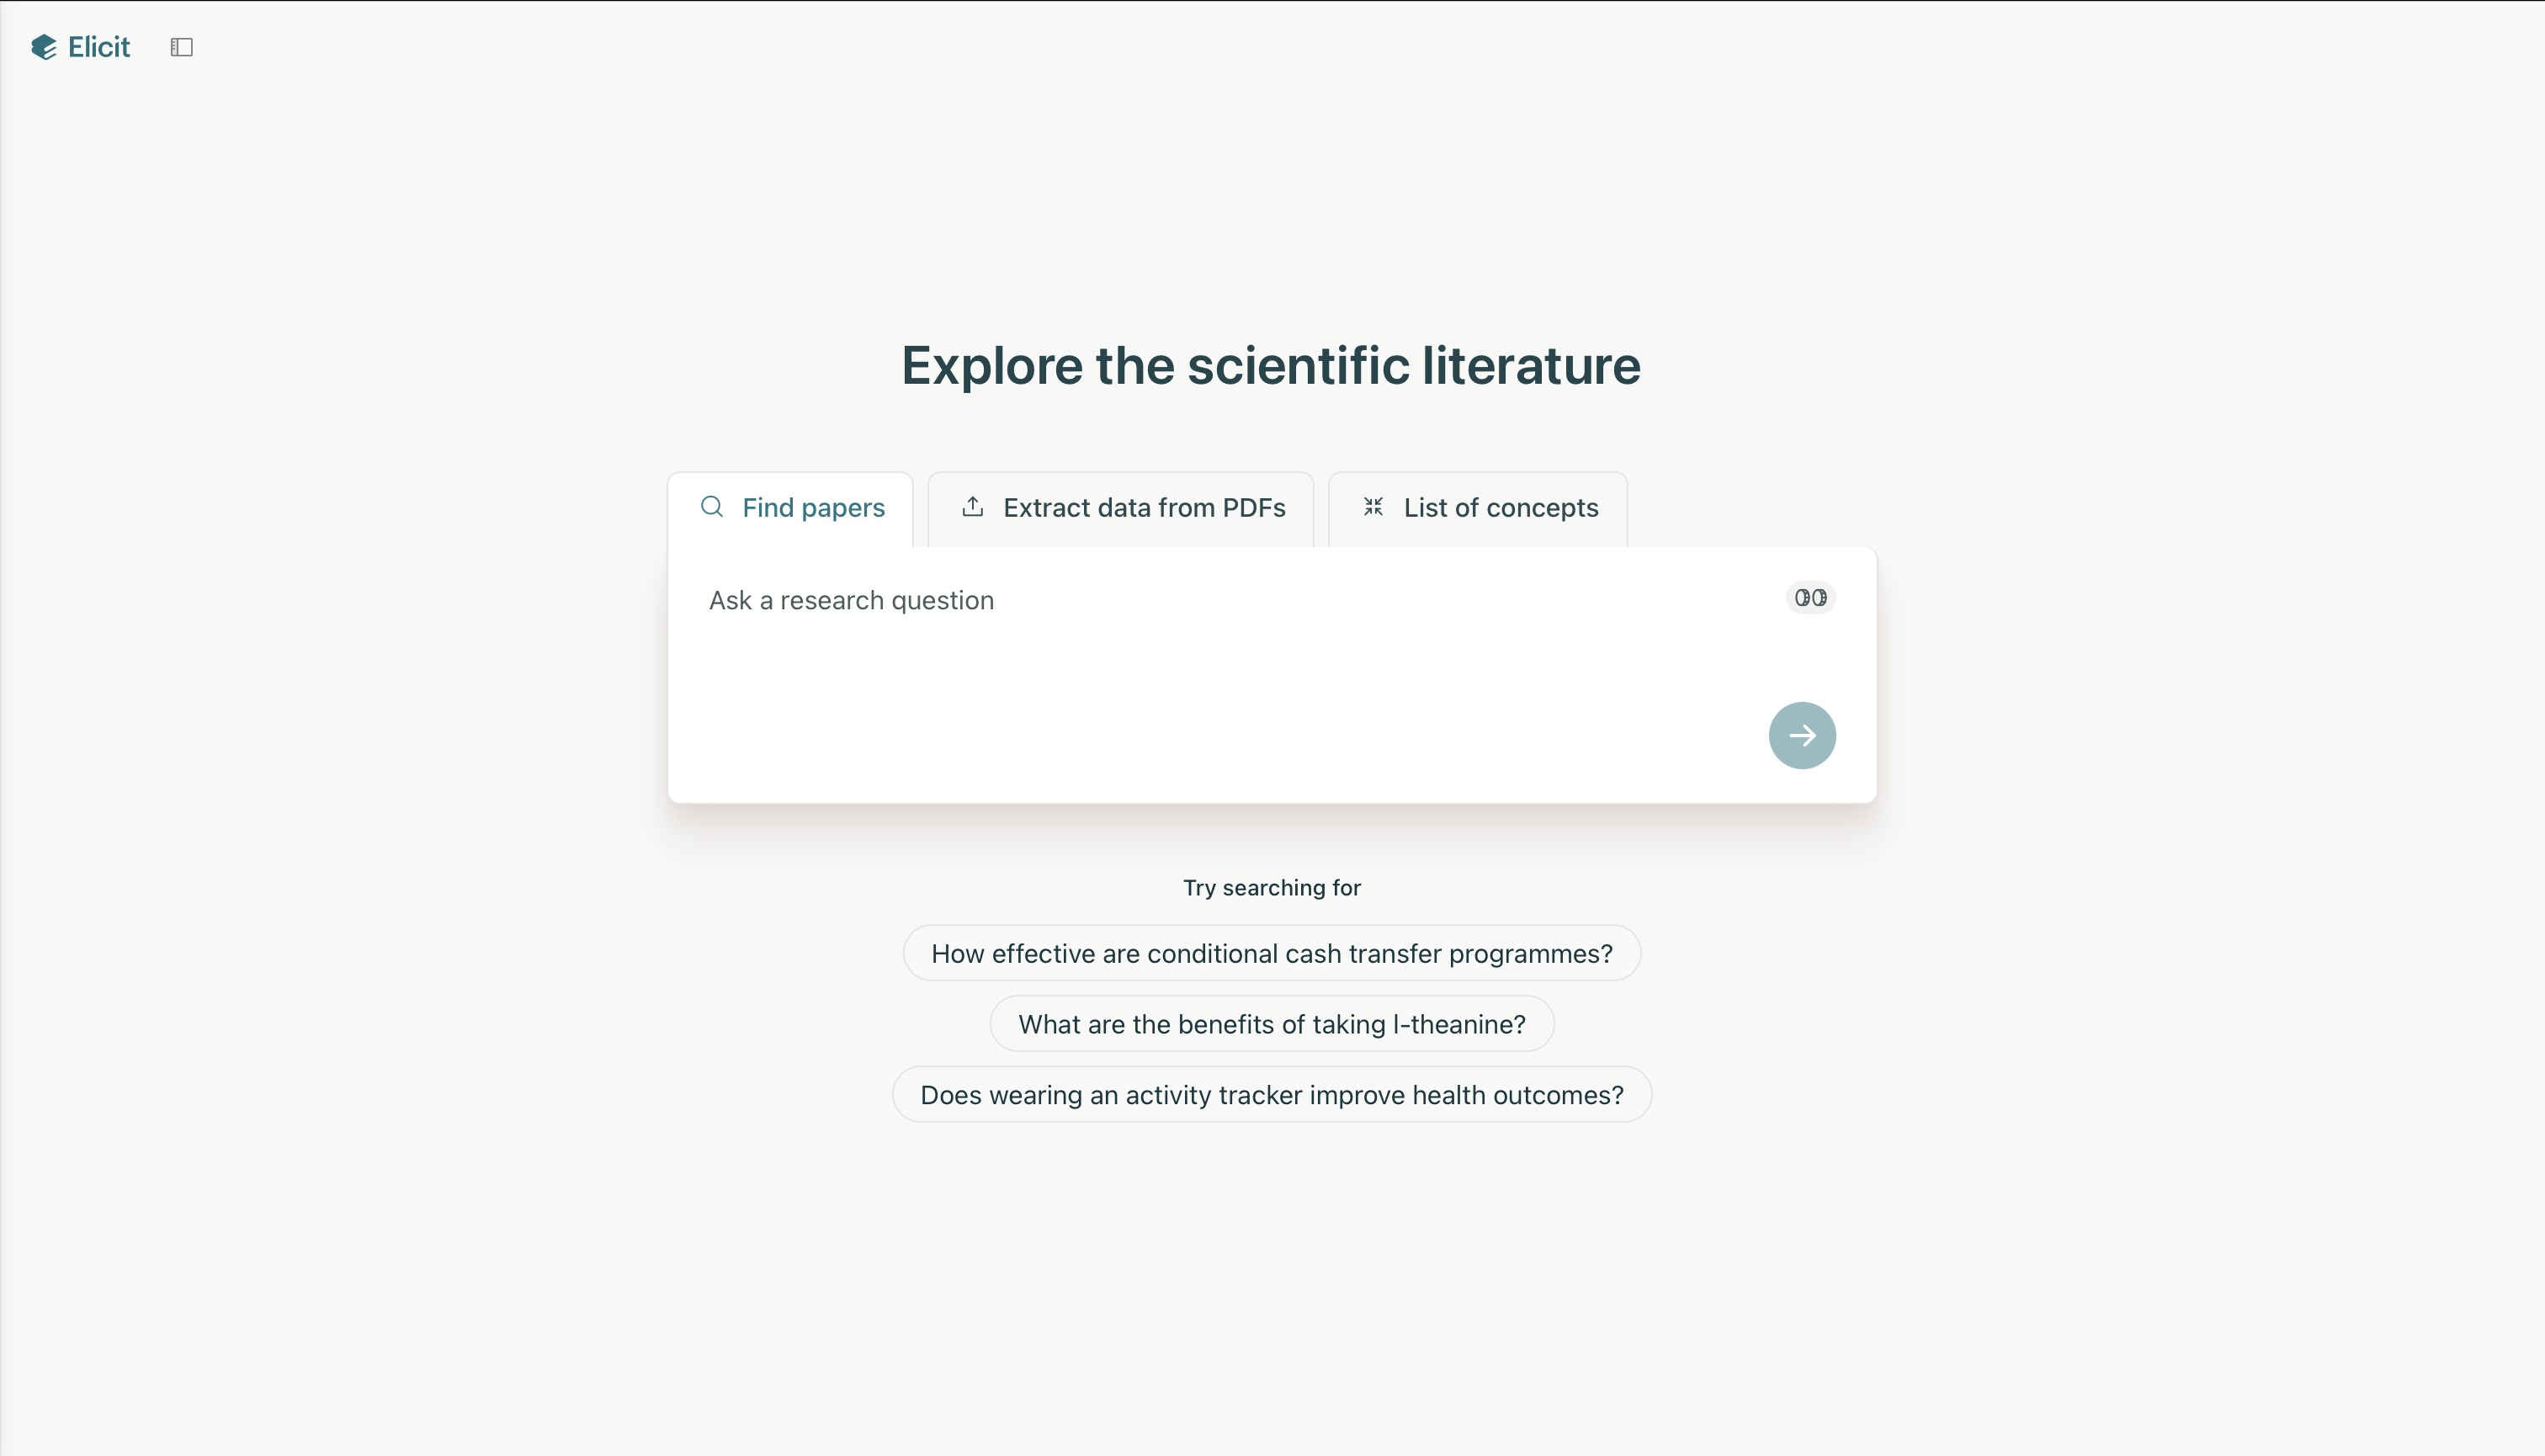
\includegraphics{images/chapitre9_image2.png}

}

\caption{\label{fig-ellicit}Menu d'accueil d'Ellicit}

\end{figure}%

Par exemple, disons que je m'intéresse à la question suivante: Qu'est-ce
que la démocratie? Cependant, je ne sais par où commencé pour me faire
une tête sur le sujet. \emph{Ellicit} offre une solution à ce problème.
La Figure~\ref{fig-ellicit} correspond au menu d'accueil du site web.
Une fois là, je n'aurais qu'à écrire ma question dans la case «
\emph{Ask a research question} ». Les résultats générés sont représentés
dans la Figure~\ref{fig-results1} et Figure~\ref{fig-results2}

\begin{figure}

\begin{minipage}{0.50\linewidth}

\begin{figure}[H]

\centering{

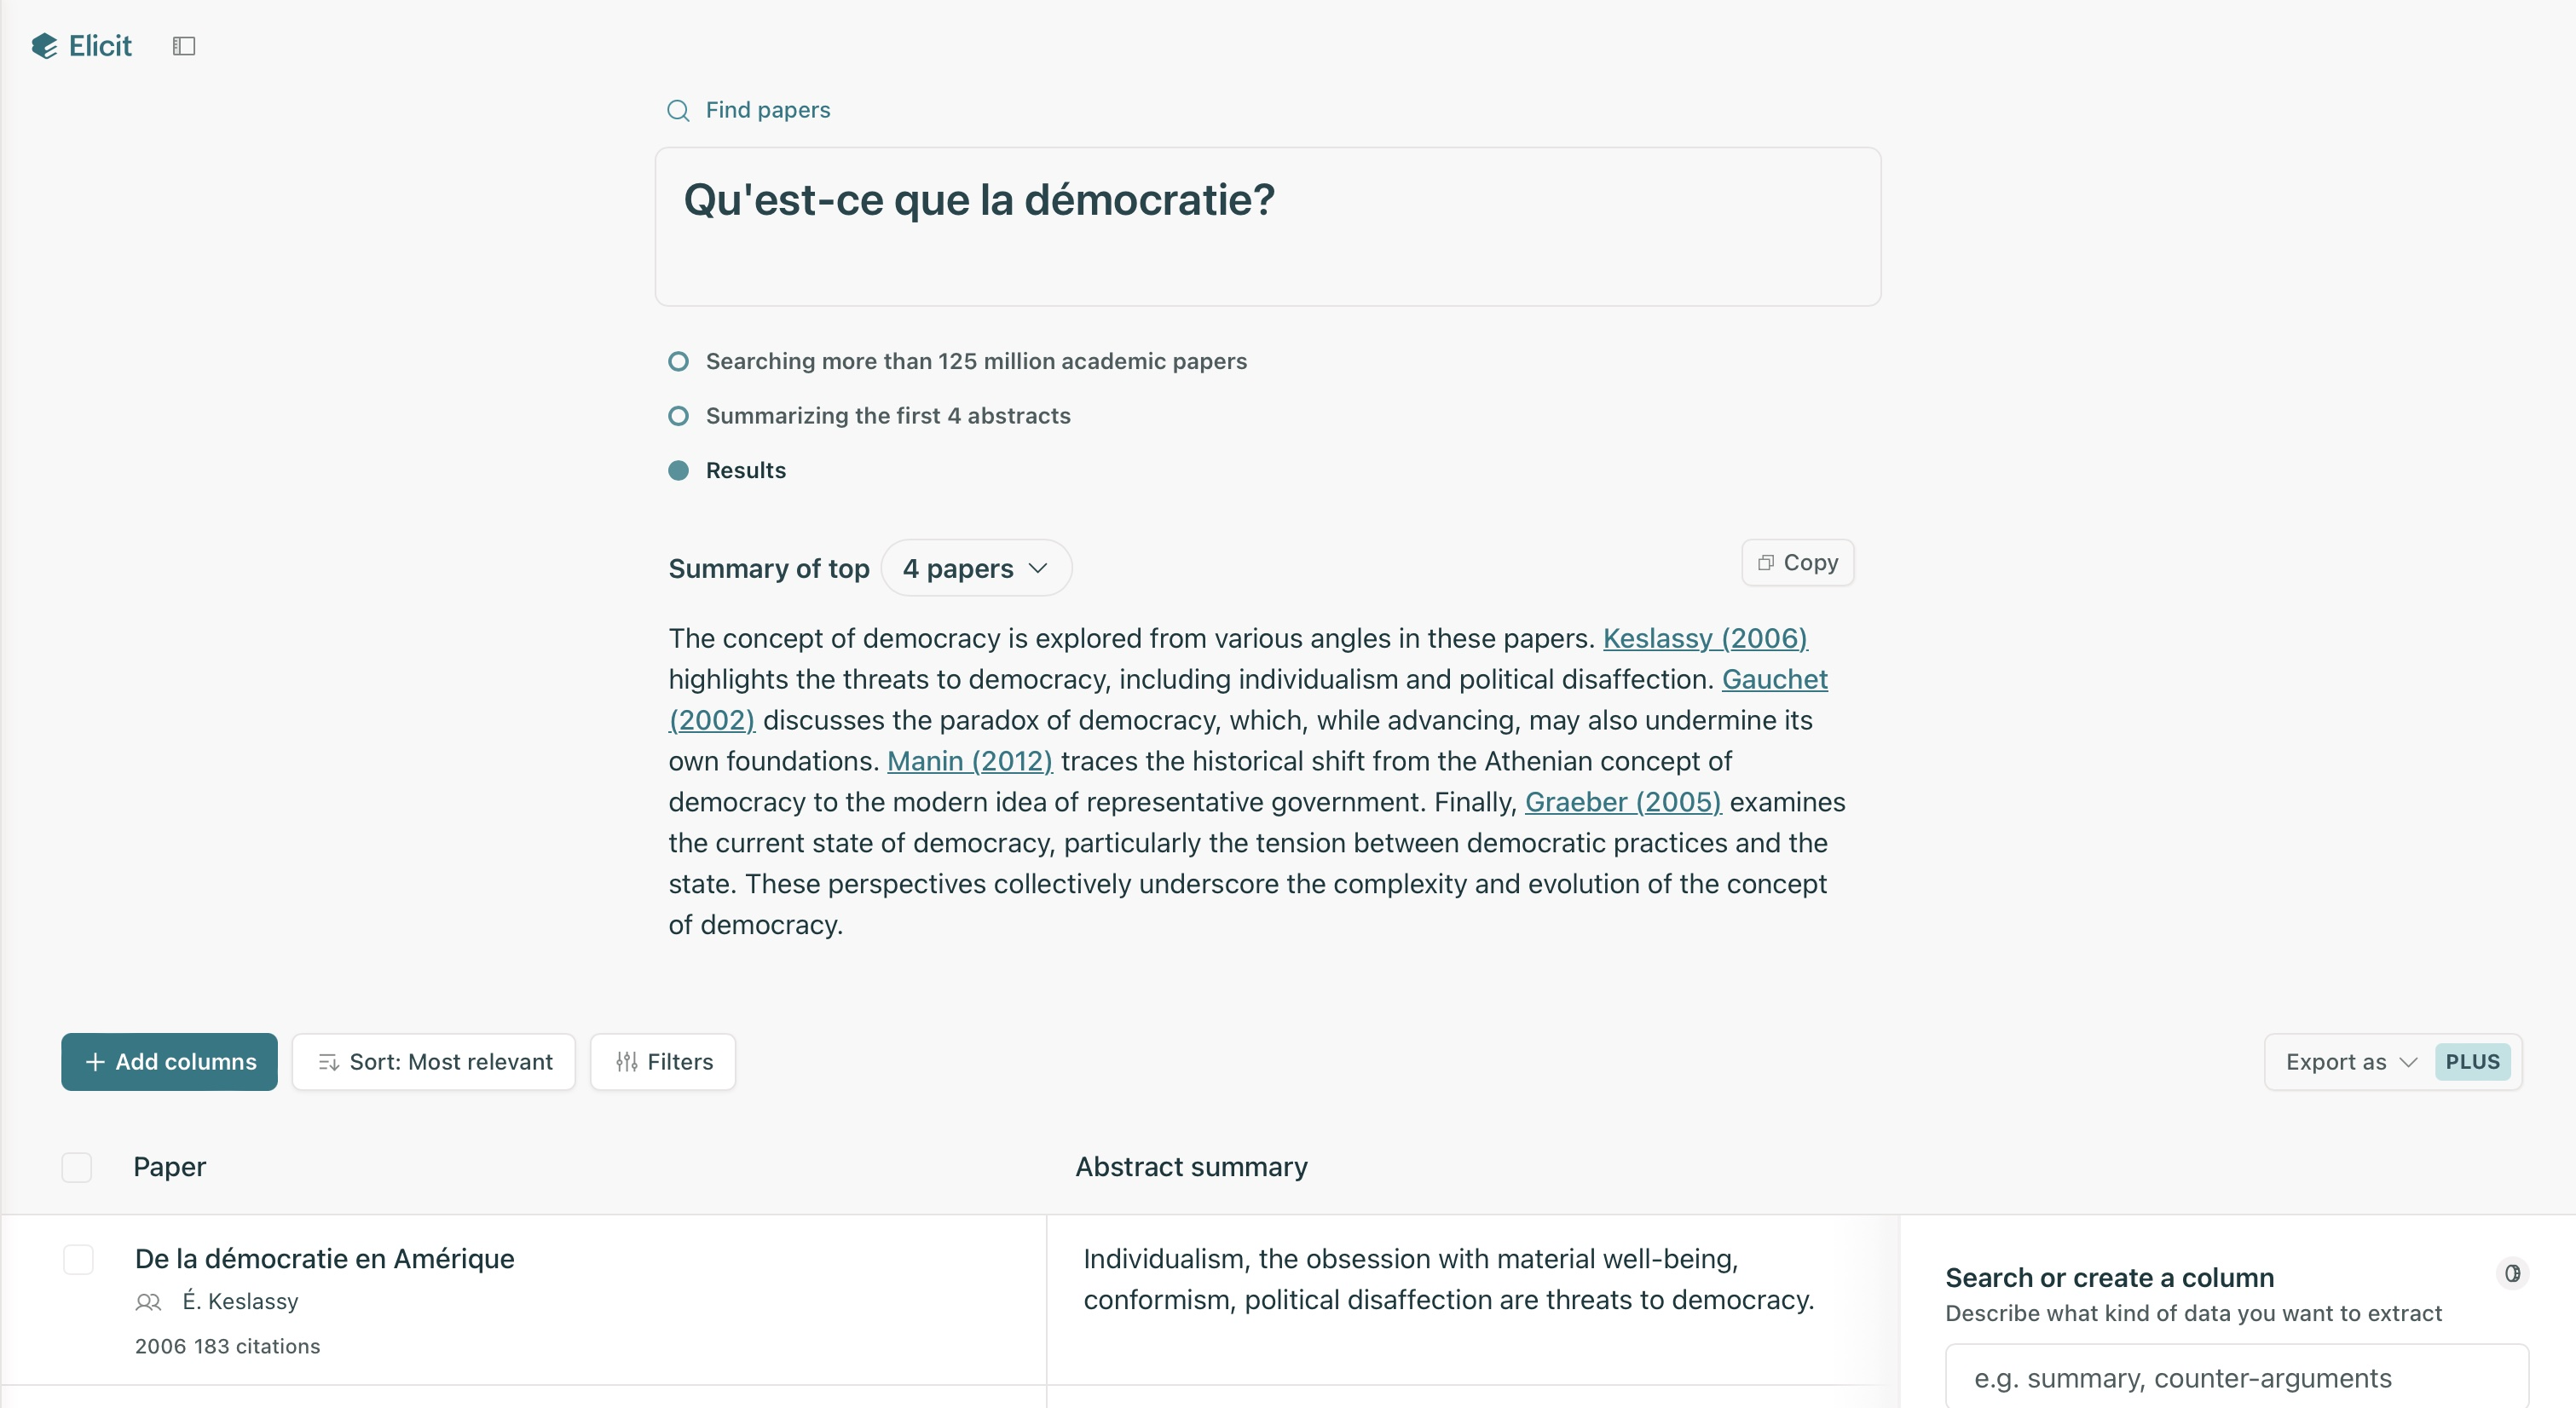
\includegraphics{images/chapitre9_image3.png}

}

\caption{\label{fig-results1}Court résumé du sujet}

\end{figure}%

\end{minipage}%
%
\begin{minipage}{0.50\linewidth}

\begin{figure}[H]

\centering{

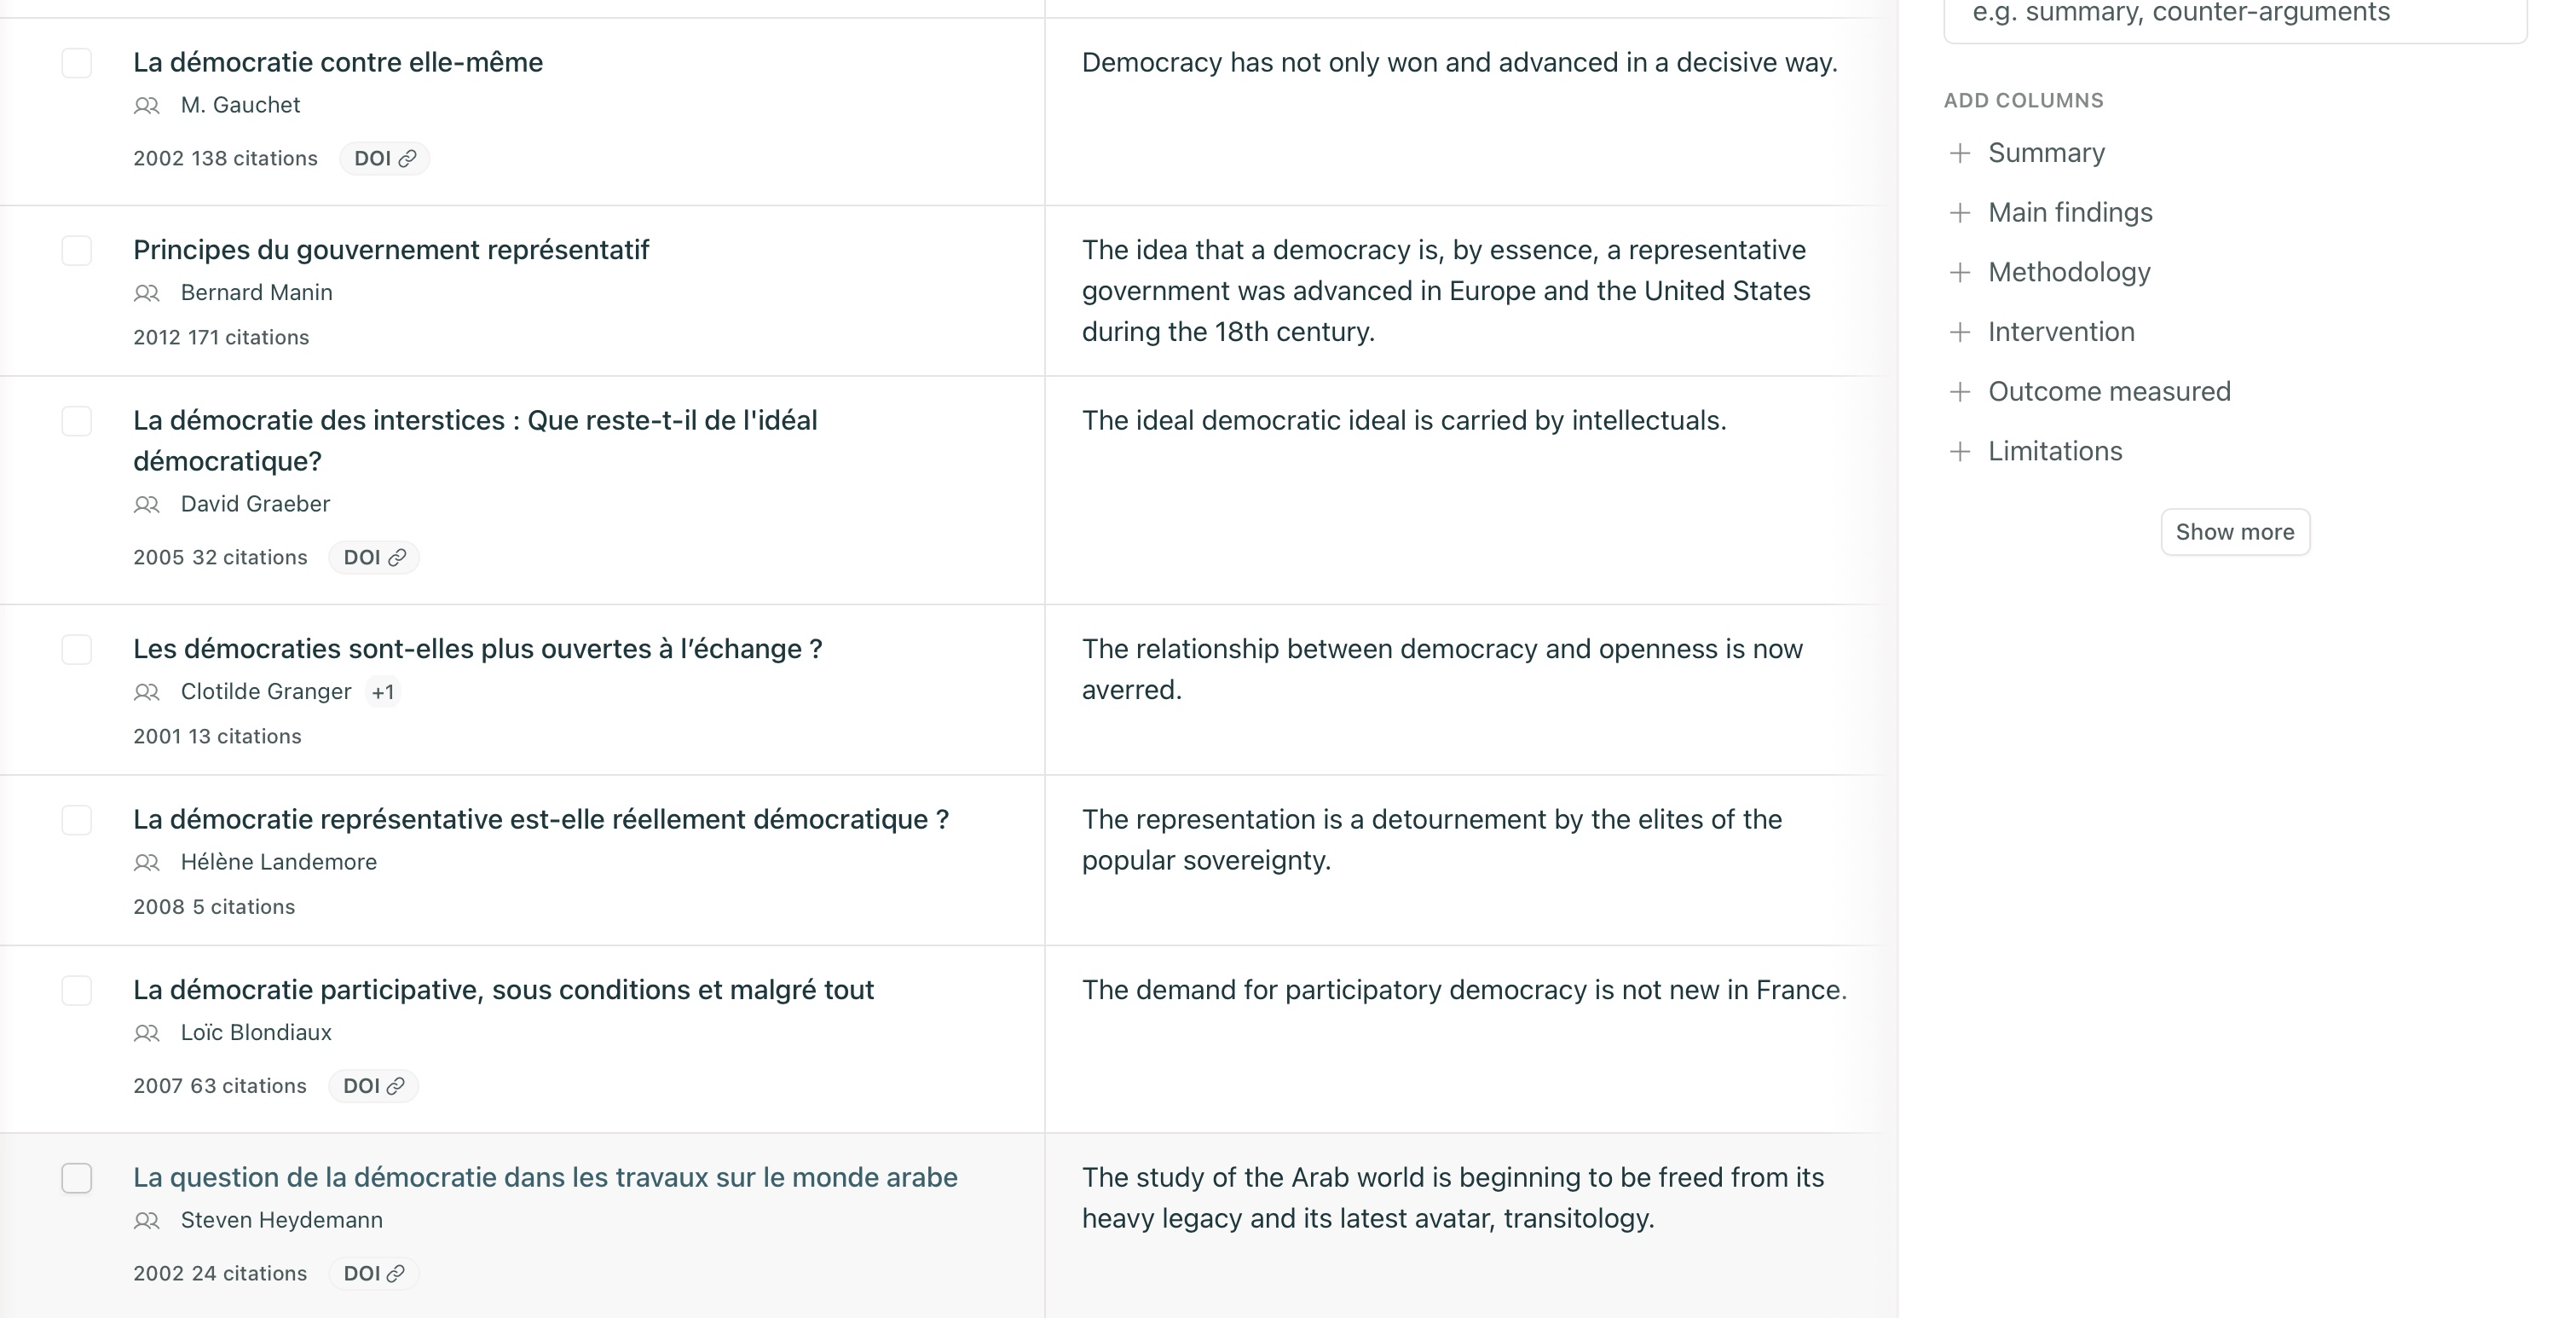
\includegraphics{images/chapitre9_image4.png}

}

\caption{\label{fig-results2}Suggestions de lectures}

\end{figure}%

\end{minipage}%

\end{figure}%

Le logiciel offre donc un moyen intéressant afin de faire un premier «
filtrage » de la littérature sur un sujet, tout en fournissant un résumé
des sources suggérées à partir desquelles nous pouvons juger de sa
pertinence en fonction de nos besoins.

Cependant, il est fortement recommandé d'utiliser le résumé produit par
le logiciel, dans la Figure~\ref{fig-results1}, et ceux de chaque
suggestion, dans la Figure~\ref{fig-results2}, à titre indicatif et
uniquement pour notre propre réflexion. En d'autres termes, \textbf{ne
jamais faire un copier-coller de ces résumés afin de les inclures dans
notre travail de recherche}. Ce logiciel doit impérativement être
accompagné d'une utilisation intègre de la littérature. Une bonne
utilisation de ce logiciel devrait se limiter à trouver des articles
et/ou des livres scientifiques selon nos besoins, que nous consulterons
par la suite pour rédiger notre revue des écrits et trouver des
références supplémentaires.

Un autre outils soffre à nous afin de trouver des références
supplémentaires: \emph{Research Rabbit}. Ce logiciel est gratuit, mais
demande de se créer un compte afin de pouvoir utiliser ses services. Une
fois que j'ai lu plusieurs articles et/ou chapitres de livre, et que
j'ai incorporé les documents dans Zotero, je peux importer mon fichier
contenant mes références dans \emph{Research Rabbit}. La
Figure~\ref{fig-rr1} présente le menu principal du site web.

\begin{figure}

\centering{

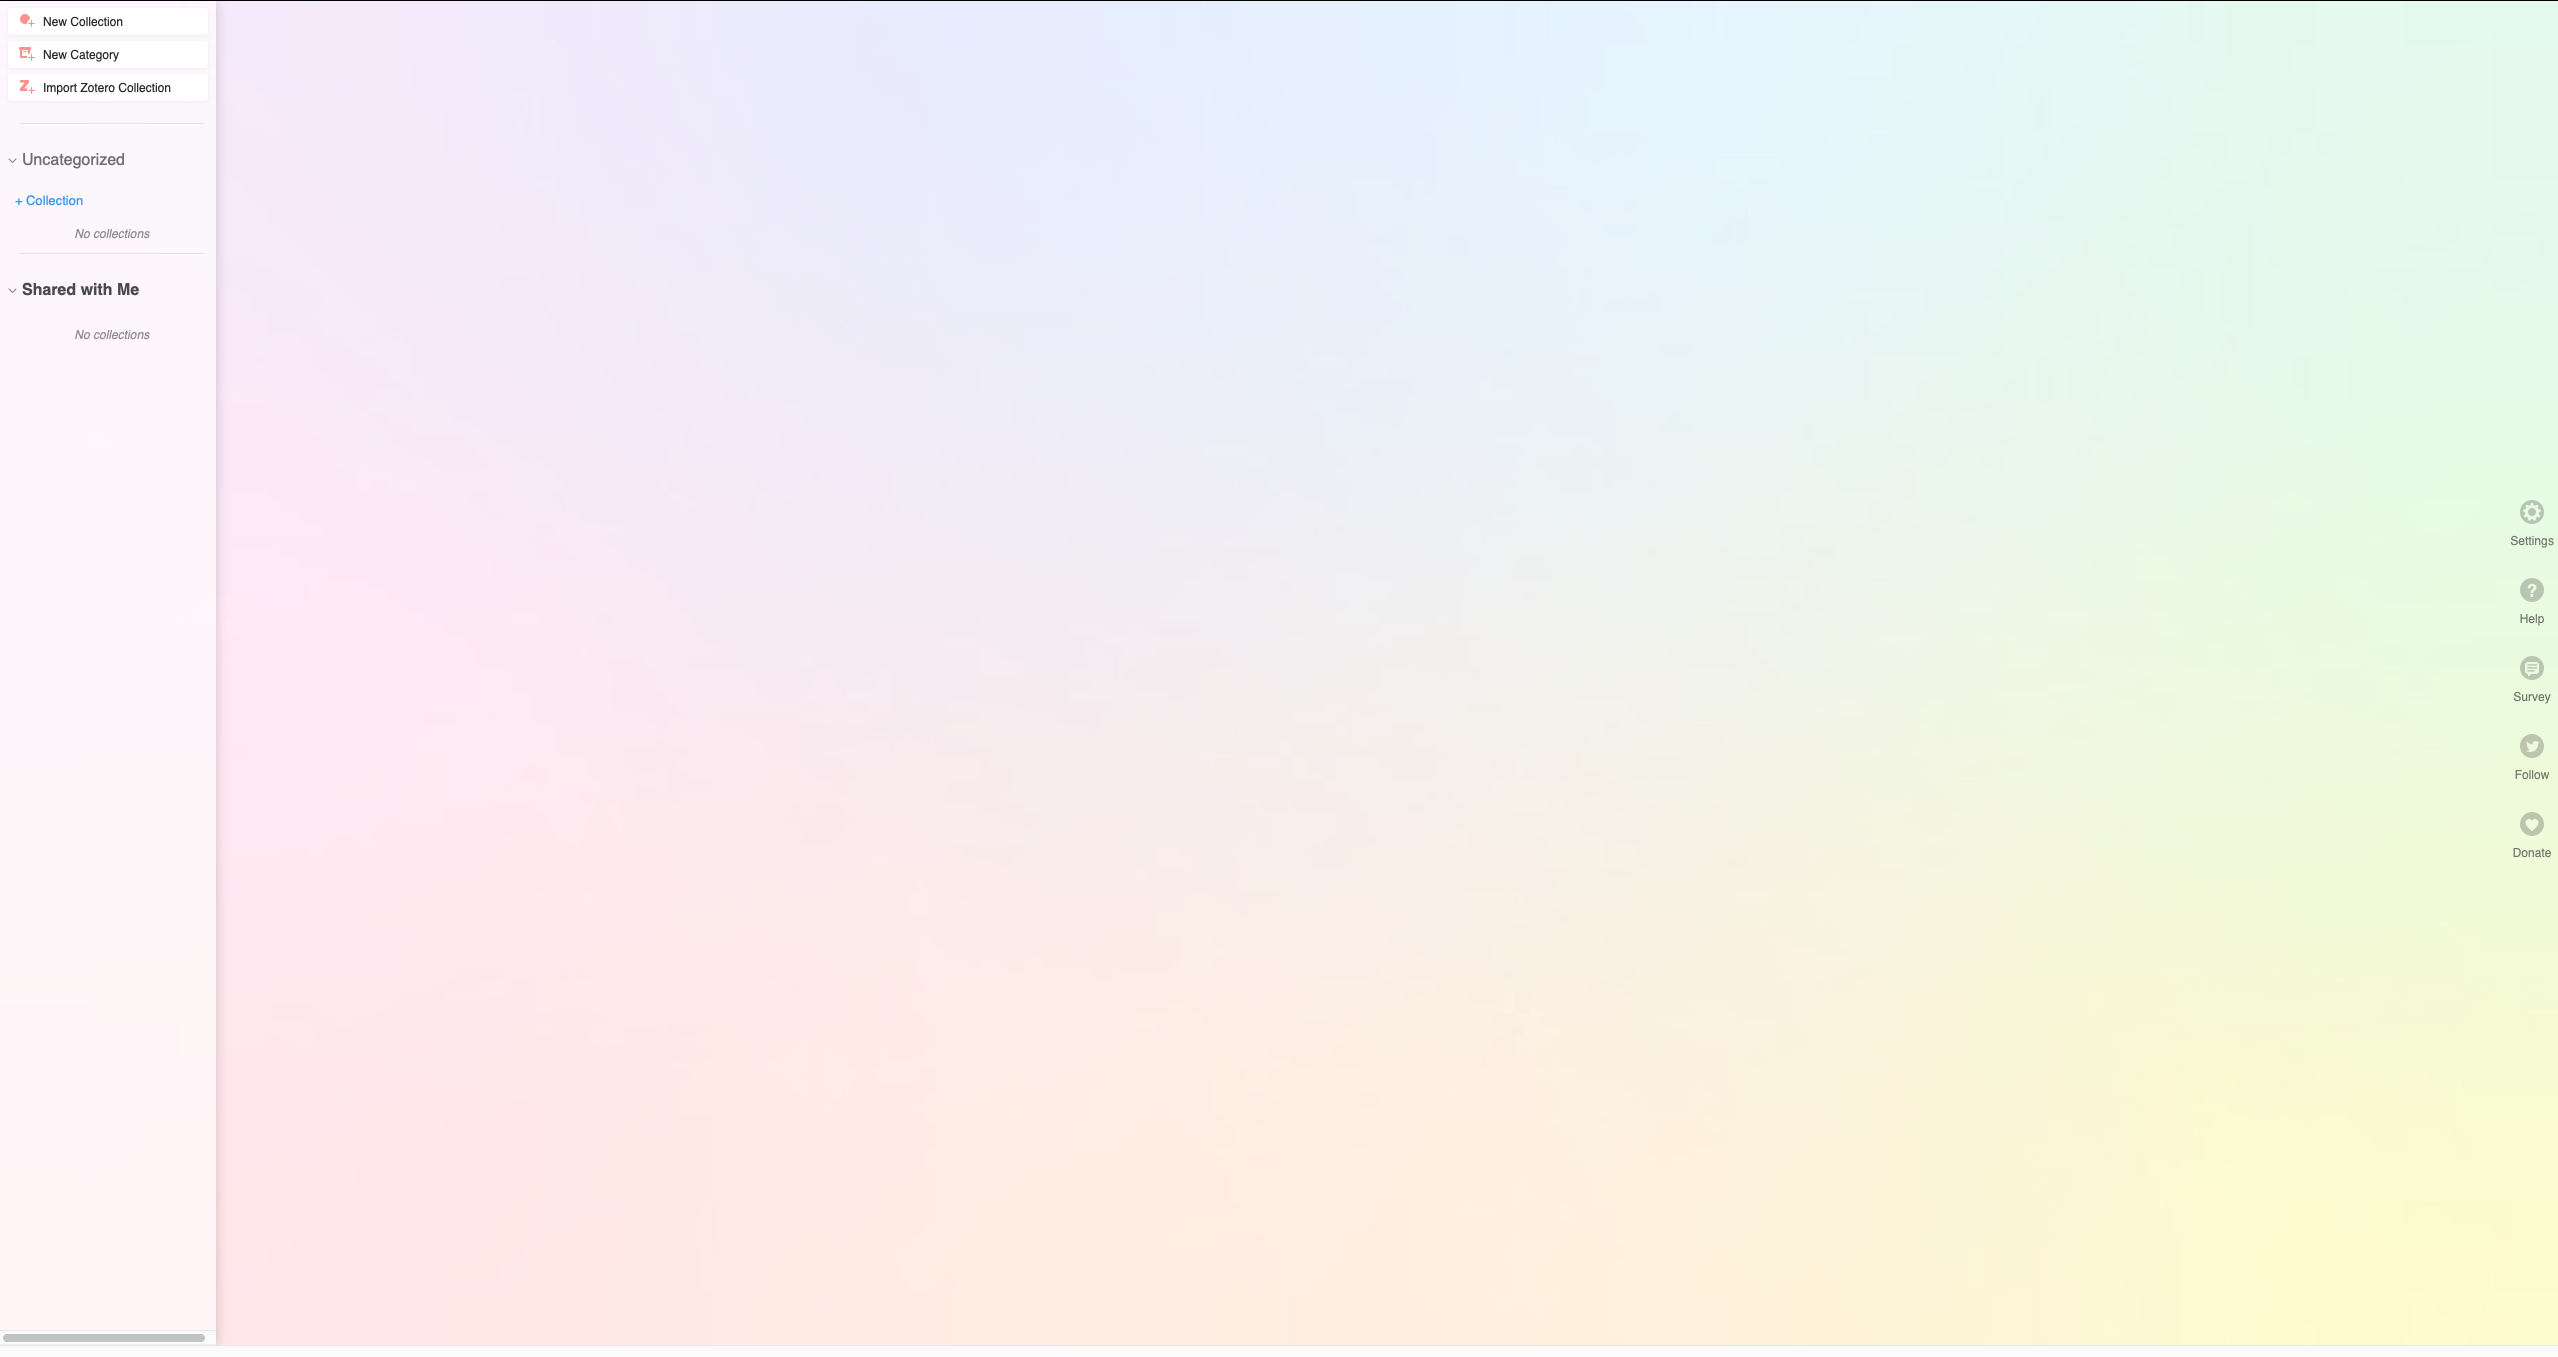
\includegraphics{images/chapitre9_RR1.png}

}

\caption{\label{fig-rr1}Menu principal}

\end{figure}%

\begin{figure}

\centering{

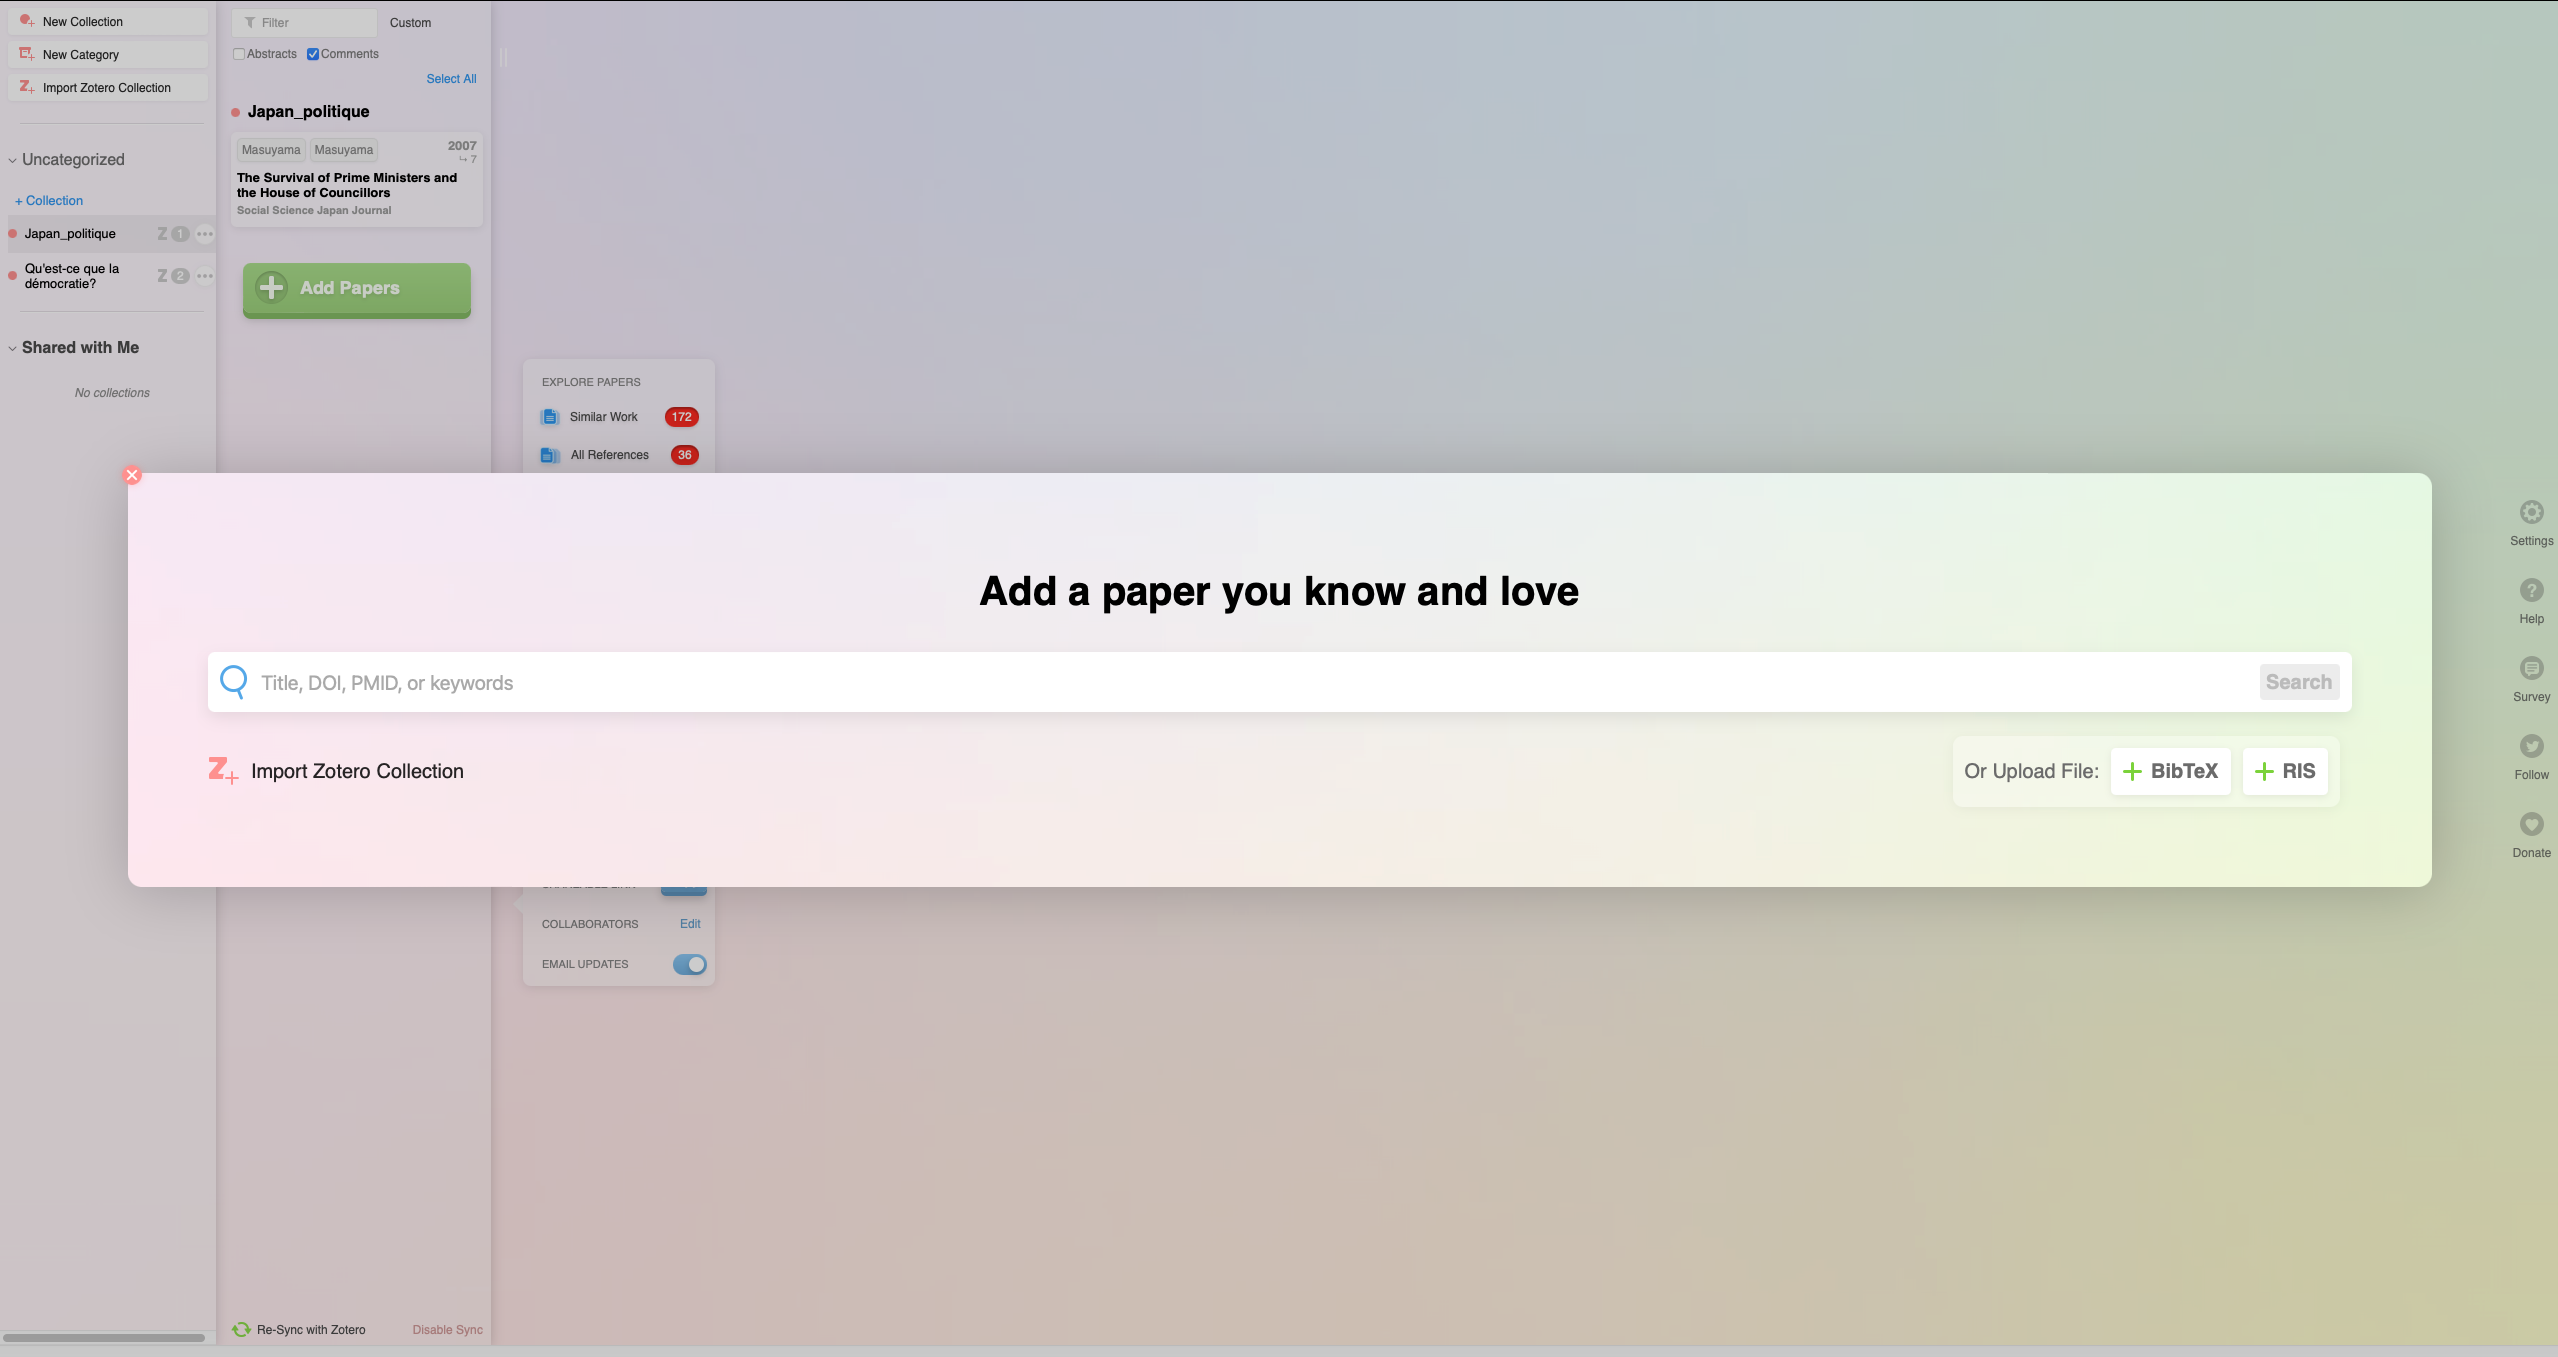
\includegraphics{images/chapitre9_rr2.png}

}

\caption{\label{fig-rr2}Importation manuelle de documents}

\end{figure}%

\begin{figure}

\centering{

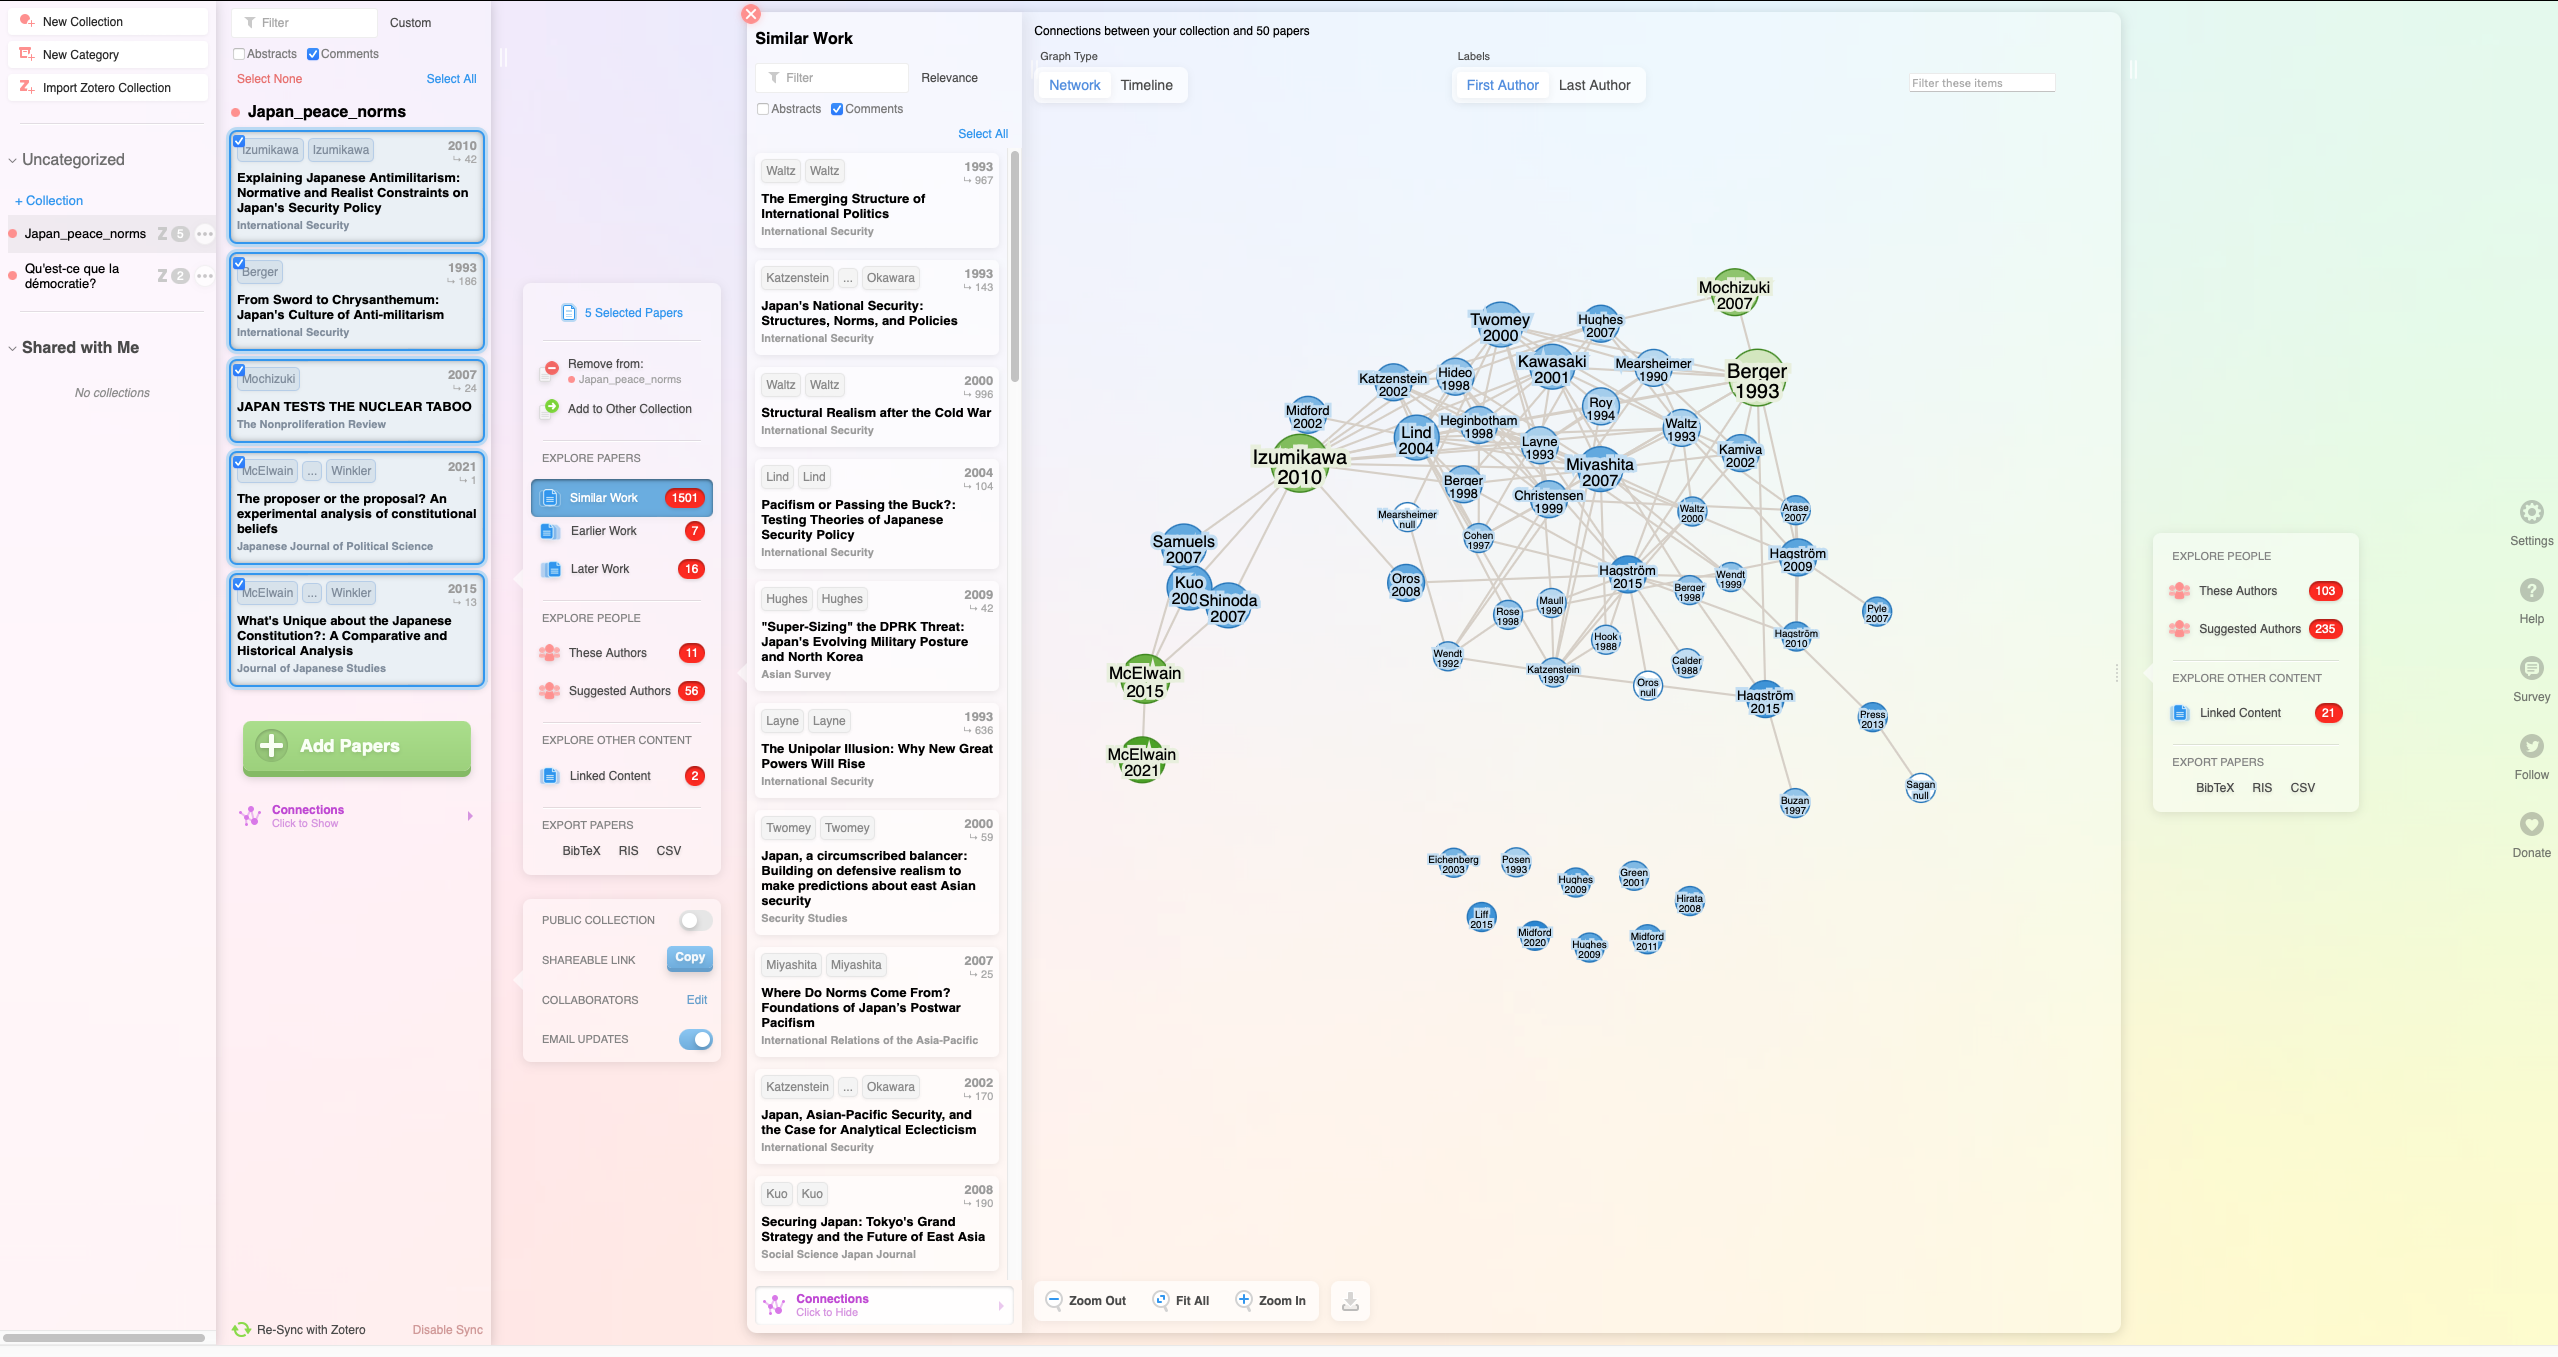
\includegraphics{images/chapitre9_RR3.png}

}

\caption{\label{fig-rr3}Présentation de la littérature similaire}

\end{figure}%

\begin{figure}

\centering{

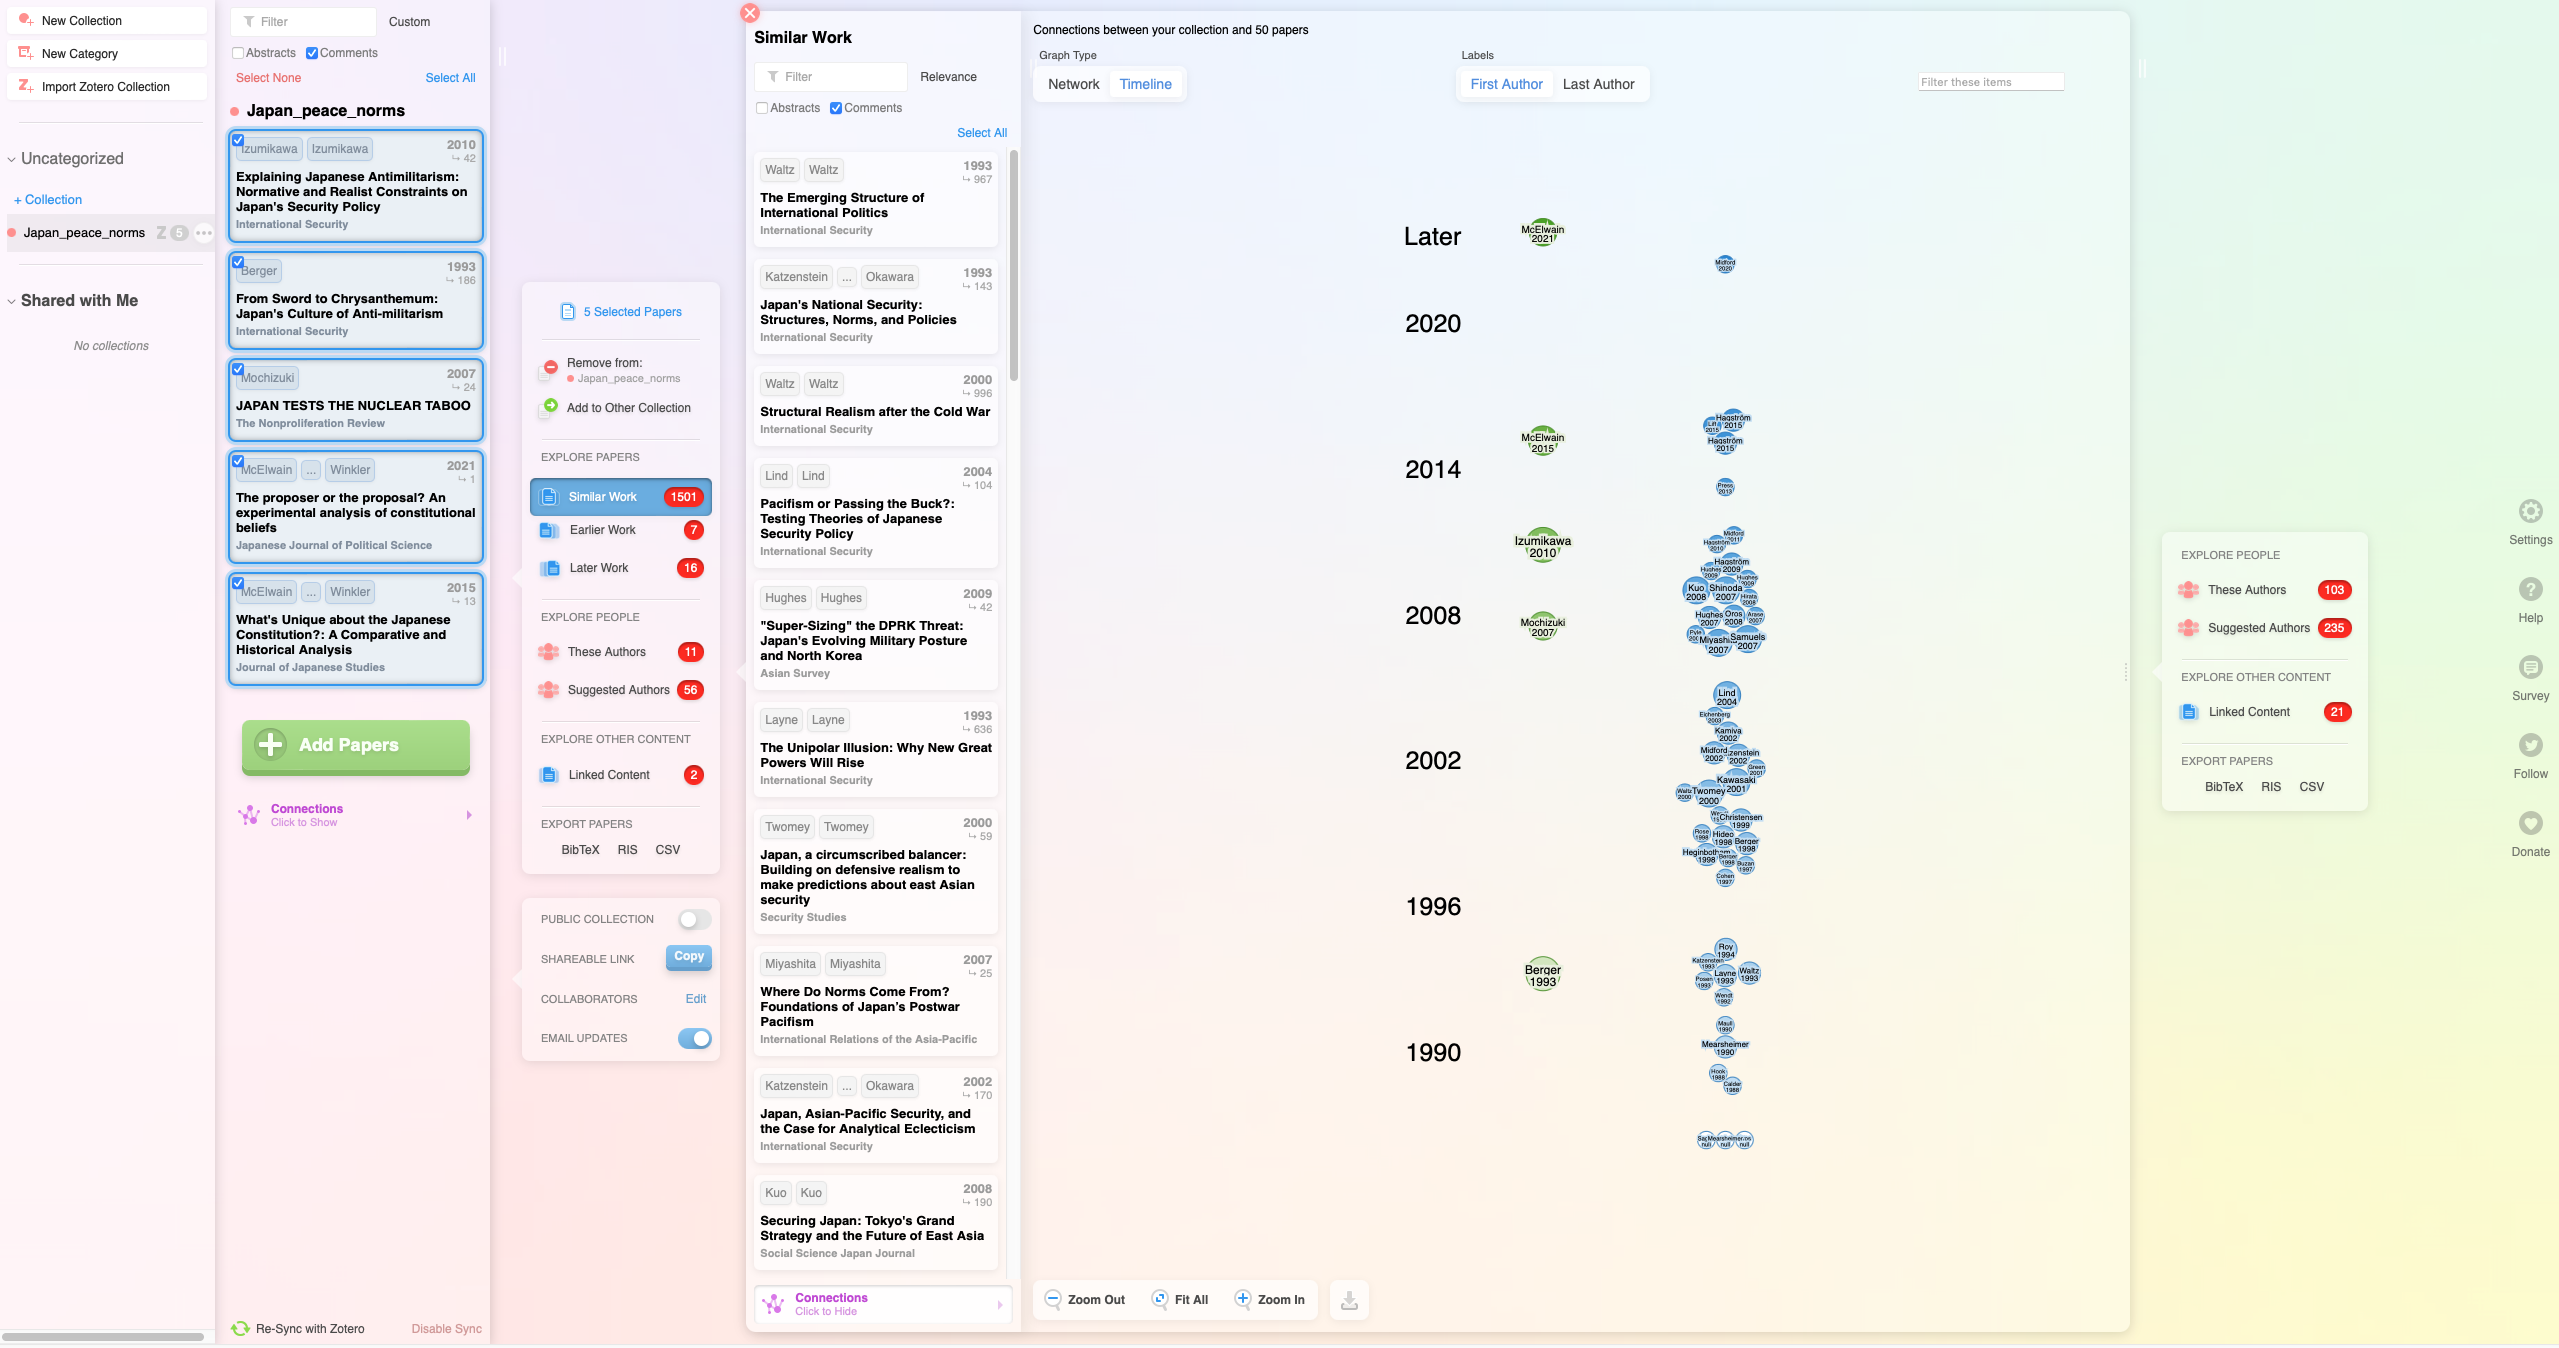
\includegraphics{images/chapitre9_rr4.png}

}

\caption{\label{fig-rr4}Vue « Timeline » des références}

\end{figure}%

Avant toute chose, \emph{Research Rabbit} doit être considéré comme un
outils qui m'aidera à \emph{complémenter} ma revue des écrits. En
d'autres termes, afin que ce logiciel soit utile, il faut déjà avoir des
articles sous la main. \emph{Ellicit} peut nous aider pour cette tâche,
mais aussi il est pratique de consulter des \emph{handbooks}\footnote{Il
  s'agit d'ouvrages généraux qui porte sur un sujet quelconque. Les
  éditeurs les plus connus sont notamment \emph{Oxford}, \emph{SAGE} et
  \emph{Routledge}.} afin de se faire une idée sur le sujet qui nous
intéresse en plus de trouver des références. Au besoin, les
bibliothécaires des différents départements universitaires sont aussi
d'excellente ressource pour débuter une recherche.

Utilisons un exemple concret afin d'illustrer l'utilisation de
\emph{Research Rabbit}. Disons que nous nous intéressons à la question
suivante: quel est le rôle des normes pacifistes sur les processus
politiques au Japon? Après une rapide recherche, je trouve ces articles
qui semblent chaucn éclairer un aspect particulier à propos de cette
question. Une fois qu'ils ont été importé dans Zotero et qu'ils ont été
lu, je peux importé ma collection Zotero dans \emph{Research Rabbit} en
cliquant sur le bouton \emph{Import Zotero Collection}, situé dans le
coin supérieur gauche de la Figure~\ref{fig-rr1}. Il se peut que le
logiciel ne trouve pas tous les articles que nous avons dans notre
collection Zotero. Une alternative est de cliquer sur le bouton vert
\emph{Add Paper} situé dans la colone de notre collection. La
Figure~\ref{fig-rr2} montre la barre de recherche qui apparaitra, et
dans laquelle on pourra ajouter manuellement les articles au besoin. Une
fois que nous aurons ajouter les premiers articles que nous aurons lu,
\emph{Research Rabbit} pourra nous dresser une « cartographie » des
différentes sources qui sont en lien avec les articles que j'aurai lu.
La Figure~\ref{fig-rr3} présente cette cartographie.

Nous avons trois possibilités afin de trouver des articles
supplémentaires. La première, est de consulter les « Similar Word ».
Cette option est intéressante afin de visualiser tous les articles qui
sont près de mon sujet, et pour voir comment ils sont liés entre eux.
Les points en vert sont les sources qui font parties de ma collection.
Cependant, ce n'est pas l'option la plus recommandées. Comme nous
pouvons le voir dans la Figure~\ref{fig-rr3}, en fonction des cinq
articles que j'ai importé dans Zotero, il y a 1 501 articles similaires.
Ce qui complique la tâche de ciblage. Une deuxième option est d'utiliser
« Earlier Work » et « Later Work », surtout avec la vue « Timeline »
comme dans la Figure~\ref{fig-rr4}.

Une troisième option est de sélectionner une seule source à la fois, et
de consulter les deux options suivantes: « All References » et « All
Citations ». Elles permettent, respectivement, de visualiser tous les
articles qui sont cités dans l'article que nous avons lu, et de
visualiser les articles qui ont cité celui que nous avons lu. Ces
options sont donc très utiles pour passer au « peigne fin » chacun de
nos articles afin de dénicher des sources supplémentaires selon la
méthode « boule de neige ». Cependant, il faut faire attention dans
notre utilisation de cette méthode. Il y a un risque « d'effet tunnel »,
soit que notre revue des écrits manque de largeur et de représentativité
des différentes recherche sur le sujet. C'est pourquoi il est important
de diversifier ces sources et d'utiliser ces deux options d'une façon
complémentaire avec plusieurs articles différents. Il est donc utile
d'ajouter au fur et à mesure ses sources dans \emph{Research Rabbit}
afin de visualiser la couverture de notre revue des écrits.

\section{Quelle est la place du chercheur
maintenant?}\label{quelle-est-la-place-du-chercheur-maintenant}

Avec l'avènement de l'IA, il est tout à fait raisonnable de se demander
quelle est la place du chercheur aujourd'hui. L'avenir du chercheur
est-il en danger? Pourrait-on assister au développement des sciences
sociales sans chercheur humain derrière? Si tel est le cas, est-ce que
ça ne constituerait pas un paradoxe important? Est-ce que la machine est
mieux placée pour comprendre la réalité du monde sociale, ainsi que ses
mécanismes, que l'humain? D'une part, certains pensent que l'IA risque
de générer des « laboratoires autonomes » (Hanchen Wang, Tianfan Fu,
Yuanqi Du, Wenhao Gao, Kexin Huang, et al., 2023, pp.~55). Il n'est pas
difficile d'imaginer un monde où tout le processus scientifique, de la
conception jusqu'à la communication, serait fait par l'IA. Le chercheur
perdrait ainsi sa profession, et se limiterait à n'être qu'une partie de
l'auditoire vers qui les résultats sont présentés.

Bien que nous n'en sommes pas encore là, il est important de réfléchir
aux différents enjeux qui se poseraient dans une telle situation. Par
exemple, étant donné que l'IA est, pour l'instant, très opaque dans tout
le processus qui le mène de l'intrant vers le résultat, comment
pourrait-on s'assurer que la machine a pris toutes les précautions
nécessaires pour respecter les différents enjeux éthiques? A-t-elle eu
le consentement libre et éclairé de tous les participants? De plus, quel
est le niveau de confiance que nous pouvons avoir envers des résultats
dont on ne connait pas le processus qui y a mené? Sur cette dernière
question, l'une des caractéristiques fondamentales de la science est la
reproductibilité des protocoles scientifiques (Bourgeois, 2021; King et
al., 2021). Toutes les recherches doivent présenter, d'une manière très
précise, comment les données ont choisi, comment elles ont été
collectées et comment elles ont été analysées. Le terme transparence est
très important, et résume l'esprit de toute communication scientifique.
Or, c'est une limite importante de l'IA en ce moment: nous n'avons pas
accès aux processus qui mènent de l'intrant à l'extrant (Hanchen Wang,
Tianfan Fu, Yuanqi Du, Wenhao Gao, Kexin Huang, et al., 2023, pp.~56).
Cette opacité nous empêche d'évaluer correctement la validité d'un
protocole scientifique qui serait réalisée par l'IA. La conséquence
logique de cette situation est de toujours rester vigilant et de
questionner constamment les informations fournies par le robot
conversationnel. L'utilisation exclusive de tel logiciel, sans se
référer à des sources scientifiques qui ont été publiées par des revues
scientifiques ou des éditeurs scientifiques, ne devrait jamais être une
option. Il n'est pas seulement question d'intégrité et d'éthique, mais
de toute la conception de ce que constitue un savoir scientifique.
L'utilisation de ChatGPT, par exemple, pour produire un savoir
quelconque met au défi nos conceptions épistémologiques. Générer des
textes entiers avec l'aide de l'IA ne devrait donc pas être considéré.

Comme nous le voyons, l'avènement de l'IA en recherche amène des
questions et des réflexions épistémologiques\footnote{L'épistémologie
  est l'une des branches de la philosophie des sciences qui s'intéresse
  au savoir et à la connaissance. De manière générale, et très
  simplifié, l'une des questions fondamentales de l'épistémologie et de
  se questionner quant à savoir ce qu'est un savoir qui serait
  scientifique.} et méthodologiques\footnote{La méthodologie fait
  référence à la branche de la philosophie des sciences qui s'intéresse
  aux outils de collecte et d'analyse de données.} importantes. Ces
questions sont cruciales et doivent être abordées le plus rapidement
possible. En tant que chercheur, nous devons nous questionner par
rapport à l'utilisation de ces nouvelles technologies. Il faut être
proactif et initier les réflexions sur la place du chercheur maintenant.

En ce sens, il faut élargir notre perspective et dépasser la question
quant à savoir si la profession de chercheur va disparaître ou non. En
fait, il faut se questionner par rapport au rôle du chercheur. Qu'est-ce
qu'il devient à l'ère de l'intelligence artificielle? Comment se
transforme-t-il? Pour l'instant, il est encore difficile de répondre et
d'anticiper efficacement ce qui arrivera. Il n'en reste pas moins pour
autant qu'initier la réflexion est nécessaire. Encore une fois, les
universités sont des lieux privilégiés pour avoir ce genre de réflexion,
tant venant des étudiants que des enseignants.

\section{L'IA en sciences sociales}\label{lia-en-sciences-sociales}

Malgré que l'utilisation de l'IA en sciences sociales soit relativement
récente, il y a déjà quelques recherches qui se sont penchées sur son
utilisation dans un contexte scientifique. Tout d'abord, la recherche de
Peterson et al. (2021), qui s'intéresse à comprendre comment les
individus prennent des décisions, utilise l'IA afin de traiter une
importante quantité de donnée rapidement. Leur base de données est
environ trente fois plus importante que celles des études précédentes.
De plus, ils ont programmé différentes théories afin de vérifier
laquelle correspondait le mieux aux patterns présents dans les données.
L'utilisation de l'IA dans cette recherche est très intéressante
puisqu'elle permet de tester des théories existantes sur un vaste
ensemble de données, qui auraient pris beaucoup plus de temps si cela
avait été réalisé « manuellement ».

Ensuite, la recherche de Park et al. (2023) utilise l'IA pour créer des
``generative agents'' qui interagissent entre eux reproduisant des
comportements individuels et collectifs humains. Leur objectif et d'en
faire des proxys1 pour étudier le comportement humain. Leur modèle prend
la forme d'une simulation interactive, similaire au jeu vidéo Sims. Bien
que ce ne soit pas encore au point, cette application de l'IA
permettrait de tester des prototypes de systèmes sociaux ainsi que des
théories (Park et al., 2023).

Similairement, la recherche de Argyle et al. (2023) utilise ChatGPT
comme proxy pour étudier l'opinion publique certains sous-groupes
sociaux. Leur objectif est de démontrer que ChatGPT peut être utilisé,
avec un bon niveau de confiance, pour explorer et tester des hypothèses
qui seraient coûteuses si c'était fait avec des sujets humains. En
effet, le déploiement d'un sondage est toujours une sorte pari; ils sont
en général relativement coûteux, et il est difficile de prévoir si les
résultats obtenus seront significatifs. ChatGPT permettrait donc de
faire un prétest afin d'améliorer et de corriger un questionnaire avant
de le déployer sur des sujets humains.

Malgré ces avantages, il est important de souligner quelques limites
quant à l'utilisation de l'IA en sciences sociales. La limite la plus
importante est que l'IA ne remplace en aucun cas un être humain. Étant
des chercheurs en sciences sociales et sciences humaines, nous
dénaturerions nos disciplines si l'on se limitait à l'IA pour répondre à
nos questions. Par conséquent, un test réalisé avec l'IA ne pourra
jamais avoir le même niveau de confiance qu'une recherche réalisée avec
des humains. Il est donc important de limiter l'utilisation de l'IA à
des fins exploratoires. Une autre limite importante, mentionnée par Park
et al. (2023) dans leur recherche, est que l'IA peut être sujette à des
hallucinations. En d'autres termes, l'IA peut fabriquer des informations
de toute pièce (Weise \& Metz, 2023). Cela pose un sérieux problème
quant à la fiabilité des informations générées par l'IA. C'est pour
cette raison, notamment, que nous devons toujours rester vigilants. Les
conséquences d'attribuer une valeur scientifique à des informations qui
seraient fausses seraient graves. La science ne vise pas à construire
une compréhension fictive de la réalité. Une fausse compréhension des
interactions et des dynamiques sociales pourrait avoir des conséquences
vraiment importantes sur le bien-être de nos sociétés. Restons
vigilants.

\section{Conclusion}\label{conclusion-6}

En guise de conclusion, nous souhaitons lancer une dernière réflexion un
peu plus philosophique, mais tout aussi importante: le transhumanisme,
«{[}\ldots{]} un mouvement international, culturel et intellectuel,
prônant l'usage des sciences et des techniques dans le but d'améliorer
la condition humaine, notamment par l'augmentation des capacités
physiques et mentales des êtres humains » (Forestier \& Ansermet, 2021).
La question principale qui se pose est: est-ce vraiment raisonnable
d'augmenter les capacités humaines au-delà de leur limite biologique?
Surtout, que deviendront les sciences sociales et humaines si le
principal sujet d'étude, soit l'humain, n'est plus tout à fait lui-même?
Peut-on faire des sciences sociales sur des sujets qui sont que
partiellement humain? Ce qui rend les sciences sociales aussi
intéressantes et pertinentes c'est peut-être, justement, parce que
l'humain n'a pas d'essence. Pour reprendre les mots de Sartre (1996,
pp.~26), « l'existence précède l'essence ». En d'autres termes, et comme
Sartre l'explique, l'humain n'existe pas pour remplir une fonction
prédéterminée, contrairement à un crayon qui a été conçu pour remplir la
tâche spécifique d'écrire. C'est dans cette liberté, et c'est par
l'expérience, que l'humain se construit et se définit. Notre existence
en tant que scientifique du monde social et humain est possible que
grâce à cette condition fondamentale : l'absence d'une essence qui
précède l'existence. Sinon, à quoi bon étudier le monde social s'il a
une fonction prédéterminée et fixe, dans lequel les humains n'auraient
aucune agentivité?

Cependant, avec l'arrivée de l'IA et ce désir de constamment repousser
les limites humaines, ne sommes-nous pas en train de prouver à Sartre
qu'il a tort? En fait, l'humain se serait imposé une essence, soit celle
d'être une pièce indispensable pour faire fonctionner les rouages du
système capitaliste. Face à la conception de la « croissance infinie »
qui est entretenue par ce système, l'être humain a besoin de quelque
chose pour « briser » ses capacités qui elles sont limitées : «
{[}\ldots{]} un remodelage technoscientifique et biomédical des corps et
des vies, dans leur matérialité biologique même, afin d'adapter les
individus au régime capitaliste globalisé de l'accélération. » (Dévédec,
2021, pp.~100). L'IA sera-t-elle une pièce de plus vers la réalisation
de cet idéal transhumaniste?

Le propos ici n'est pas d'encourager les lecteurs à ne pas utiliser
l'IA. En fait, nous souhaitons tout simplement appeler à une certaine
prudence. Le risque que cette technologie nous pose est d'en devenir
dépendant, voir trop (Park et al., 2023). Bien qu'elle offre de nombreux
avantages, elle a aussi le piège d'offrir beaucoup de raccourcis et de
nuire à plusieurs de nos capacités intellectuelles et physiques. Il faut
donc développer un jugement critique dans notre utilisation de l'IA. Se
poser des questions sur notre utilisation personnelle de ces outils
constitue, dès aujourd'hui, le fondement des chercheurs en sciences
sociales numériques.

Toutefois, à moins que la recherche porte directement sur ChatGPT, nous
déconseillons fortement d'utiliser uniquement ce que le robot
conversationnel fournit comme réponse. Reprenons l'exemple du
totalitarisme. Dans ce cas, bien que la définition fournie soit
relativement adéquate, nous recommandons d'aller consulter des sources
académiques afin de trianguler la définition générée, d'une part, et
surtout de présenter une définition qui est reconnue par les pairs
scientifiques. Pour ce faire, il est possible d'utiliser ChatGPT. Nous
pouvons lui demander de nous fournir 5 livres qui portent sur le sujet.
À partir de ces recommandations, nous pouvons nous référer directement à
ces ouvrages et débuter notre revue des écrits. Surtout, à moins que ce
ne soit que pour vous faire une idée du contenu, n'utilisez pas ChatGPT
pour résumer un livre et utiliser le résumé pour votre travail ! Cette
pratique constitue une forme de plagiat. Aller consulter les ouvrages
directement plutôt que d'utiliser les définitions fournies par ChatGPT
fait partie des bonnes pratiques. Développer un esprit de synthèse est
fondamental pour chaque étudiant.e universitaire, ainsi que pour les
futurs chercheur.euse.s. Commencez dès maintenant à développer ces
capacités plutôt que de demander à ChatGPT de le faire à votre place.

\section{Utilisation du package
OpenAI}\label{utilisation-du-package-openai}

\subsection{Installation et chargement du
package}\label{installation-et-chargement-du-package}

\begin{Shaded}
\begin{Highlighting}[]
\FunctionTok{install.packages}\NormalTok{(}\StringTok{"openai"}\NormalTok{) }\DocumentationTok{\#\# au besoin}
\FunctionTok{library}\NormalTok{(openai)}
\end{Highlighting}
\end{Shaded}

\section{Configuration de l'API}\label{configuration-de-lapi}

Procurez vous une clé API sur le site d'OpenAI. Soyez conscient que vous
aurez besoin d'une carte de crédit pour vous inscrire et que
l'utilisation de l'API est payante. Renseignez-vous sur les modèles
disponibles et leurs frais d'utilisation. En date de la publication du
livre, le modèle de tarification d'OpenAi est de charger un prix
spécifique par 1000 tokens. Le prix des Tokens en entrée est moins élevé
que celui des tokens en sortie.

Lorsque vous aurez votre clé API, utilisez le package usethis pour la
configurer dans votre environnement R.

\begin{Shaded}
\begin{Highlighting}[]
\FunctionTok{install.packages}\NormalTok{(}\StringTok{"usethis"}\NormalTok{) }\DocumentationTok{\#\# au besoin}
\NormalTok{usethis}\SpecialCharTok{::}\FunctionTok{edit\_r\_environ}\NormalTok{()}
\end{Highlighting}
\end{Shaded}

Ajoutez la ligne suivante à votre fichier \texttt{.Renviron}.

\begin{Shaded}
\begin{Highlighting}[]
\NormalTok{OPENAI\_API\_KEY}\OtherTok{=}\NormalTok{inserez}\SpecialCharTok{{-}}\NormalTok{votre}\SpecialCharTok{{-}}\NormalTok{cle}\SpecialCharTok{{-}}\NormalTok{api}\SpecialCharTok{{-}}\NormalTok{ici}\SpecialCharTok{{-}}\NormalTok{sans}\SpecialCharTok{{-}}\NormalTok{guillemets}
\end{Highlighting}
\end{Shaded}

\section{Utilisation de l'API}\label{utilisation-de-lapi}

La fonction principale du package openai est create\_chat\_completion().
Elle prend en entrée le modèle que vous souhaitez utiliser ainsi que le
message que vous souhaitez envoyer au modèle en format list. Voici un
modèle d'utilisation de la fonction:

\begin{Shaded}
\begin{Highlighting}[]
\NormalTok{chat\_prompt }\OtherTok{\textless{}{-}} \FunctionTok{create\_chat\_completion}\NormalTok{(}
    \AttributeTok{model =} \StringTok{"gpt{-}3.5{-}turbo"}\NormalTok{,}
    \AttributeTok{messages =} \FunctionTok{list}\NormalTok{(}
        \FunctionTok{list}\NormalTok{(}
            \StringTok{"role"} \OtherTok{=} \StringTok{"system"}\NormalTok{,}
            \StringTok{"content"} \OtherTok{=} \StringTok{"You are a helpful assistant."}
\NormalTok{        ),}
        \FunctionTok{list}\NormalTok{(}
            \StringTok{"role"} \OtherTok{=} \StringTok{"user"}\NormalTok{,}
            \StringTok{"content"} \OtherTok{=} \StringTok{"Please do the following:"}\NormalTok{)}
\NormalTok{        )}
\NormalTok{    )}
\end{Highlighting}
\end{Shaded}

Le résultat de votre requête sera contenu dans l'objet chat\_prompt
formatté en JSON. Vous pouvez accéder aux variables de la même façon
qu'un dataframe normal. Le contenu de la réponse sera dans
\texttt{chat\_prompt\$choices\$content}.

Utiliser chatgpt de cette façon ouvre plein de possibilités. Appliquer
des instructions sur un ensemble d'observations à l'aide de boucles,
utiliser des fonctions pour générer des messages et les appliquer à
travers d'autres API, analyser des sites webs en temps réel en scraping
avec des paquets tels rvest, etc. Ce sera à vous de réfléchir aux
possibilités que vous souhaitez explorer.

\section{Notes}\label{notes}

\begin{itemize}
\item
  Il est possible d'accéder aux statistiques d'utilisation de token dans
  \texttt{chat\_prompt\$usage\$prompt\_tokens} et
  \texttt{chat\_prompt\$usage\$completion\_tokens}. Vous pouvez donc
  calculer le coût de votre requête en fonction du modèle que vous
  utilisez.
\item
  Ne pas oublier d'inclure .Renviron dans votre gitignore pour ne pas
  vous faire voler votre clé API.
\item
  Il est possible de créer des images avec la fonction
  create\_image(``Inserez votre texte ici'')
\item
  Il est possible d'effectuer du speech-to-text avec la fonction
  create\_transcription() et create\_translation()
\item
  Plus de documentation est disponible au
  https://irudnyts.github.io/openai/
\item
  Plus de fonctionalités sont disponibles en python mais le package R
  est suffisant pour la plupart des utilisations.
\end{itemize}

\section{Annexe 1}\label{annexe-1}

Bonnes pratiques d'utilisation Harvard. 2023. « Guidelines for using
ChatGPT and other Generative AI tools at Harvard ».
https://provost.harvard.edu/guidelines-using-chatgpt-and-other-generative-ai-tools-harvard

MIT. 2023. « Advice and responses from faculty on ChatGTP and
A.I.-assisted writing ».
https://cmsw.mit.edu/advice-and-responses-from-faculty-on-chatgpt-and-a-i-assisted-writing/

\section{Annexe 2}\label{annexe-2}

Q : Qu'est-ce que le totalitarisme? R : Le totalitarisme est un système
politique et idéologique caractérisé par un contrôle absolu et
centralisé du gouvernement sur tous les aspects de la vie publique et
privée d'une société. Dans un régime totalitaire, le gouvernement exerce
un pouvoir autoritaire et oppressif, limitant sévèrement les libertés
individuelles, supprimant les droits de l'homme, et éliminant ou
réprimant toute opposition ou critique.

Bonnes pratiques d'utilisation Harvard. 2023. « Guidelines for using
ChatGPT and other Generative AI tools at Harvard ».
https://provost.harvard.edu/guidelines-using-chatgpt-and-other-generative-ai-tools-harvard

MIT. 2023. « Advice and responses from faculty on ChatGTP and
A.I.-assisted writing ».
https://cmsw.mit.edu/advice-and-responses-from-faculty-on-chatgpt-and-a-i-assisted-writing/

\section{Annexe 2}\label{annexe-2-1}

Q : Qu'est-ce que le totalitarisme? R : Le totalitarisme est un système
politique et idéologique caractérisé par un contrôle absolu et
centralisé du gouvernement sur tous les aspects de la vie publique et
privée d'une société. Dans un régime totalitaire, le gouvernement exerce
un pouvoir autoritaire et oppressif, limitant sévèrement les libertés
individuelles, supprimant les droits de l'homme, et éliminant ou
réprimant toute opposition ou critique.

Les caractéristiques clés du totalitarisme comprennent :

\begin{enumerate}
\def\labelenumi{\arabic{enumi}.}
\item
  \textbf{Contrôle gouvernemental absolu :} Le gouvernement exerce un
  contrôle total sur tous les aspects de la vie, y compris l'économie,
  la culture, l'éducation, les médias, la religion et les activités
  sociales.
\item
  \textbf{Idéologie dominante :} Le régime totalitaire est basé sur une
  idéologie spécifique qui est imposée à la population. Cette idéologie
  est souvent promue comme la seule vérité et toute forme de pensée
  dissidente est sévèrement réprimée.
\item
  \textbf{Culte de la personnalité :} Les dirigeants du régime
  totalitaire sont souvent présentés comme des figures quasi-divines ou
  héroïques, et un culte de la personnalité est créé autour d'eux pour
  renforcer leur autorité.
\item
  \textbf{Répression politique :} Toute forme d'opposition politique est
  réprimée de manière brutale. Les opposants sont souvent emprisonnés,
  torturés, voire exécutés. La surveillance et la dénonciation sont
  courantes pour empêcher toute critique du régime.
\item
  \textbf{Propagande intensive :} Le gouvernement contrôle les médias et
  utilise la propagande pour manipuler l'opinion publique, répandre sa
  vision du monde et justifier ses actions.
\item
  \textbf{Absence de droits individuels :} Les droits individuels tels
  que la liberté d'expression, la liberté de la presse, le droit de
  réunion et d'association sont souvent supprimés au profit de la
  suprématie de l'État.
\item
  \textbf{Contrôle de l'éducation :} L'éducation est utilisée pour
  propager l'idéologie du régime et façonner la mentalité des citoyens
  conformément à ses objectifs.
\item
  \textbf{Utilisation de la terreur :} La terreur et l'intimidation sont
  utilisées pour maintenir le contrôle sur la population. Les purges et
  les arrestations arbitraires sont fréquentes pour maintenir un climat
  de peur.
\end{enumerate}

Des exemples historiques de régimes totalitaires incluent l'Allemagne
nazie sous Adolf Hitler, l'Union soviétique sous Joseph Staline, et la
Chine sous Mao Zedong. Le totalitarisme est généralement considéré comme
une forme extrême et oppressive de gouvernement, en contraste avec les
systèmes démocratiques qui mettent l'accent sur les libertés
individuelles, la séparation des pouvoirs et la participation citoyenne.

\{\textless\textless{} pagebreak \textgreater\textgreater\}

\bookmarksetup{startatroot}

\chapter{À voir}\label{uxe0-voir}

\section{Défis et enjeux éthiques de l'IA, focus sur
ChatGPT}\label{duxe9fis-et-enjeux-uxe9thiques-de-lia-focus-sur-chatgpt}

En tant qu'étudiant, professeur, professionnel ou chercheur, il faut se
questionner par rapport à notre propre utilisation des différents outils
de l'IA. Tout d'abord, il est important de comprendre qu'il y a plus de
questions que de réponses pour l'instant. Face à ce constat, nous
n'avons pas la prétention d'être en mesure de cibler toutes les
questions qui émergent actuellement, et encore moins d'avoir les
réponses. Cependant, cela ne justifie pas pour autant d'être passif.
Nous devons essayer d'être réflexifs et critiques dans la limite de nos
capacités et de nos connaissances. En ce sens, les étudiants et les
enseignants doivent aussi être proactifs en entreprenant les démarches
nécessaires ainsi qu'en s'engageant dans la réflexion.

Dans un premier temps, un bon usage de ces outils débute avec une bonne
réflexion quant à leur utilisation. Par conséquent, les universités
constituent des endroits privilégiés pour favoriser les discussions et
les réflexions quant à l'utilisation de ces technologies. D'ailleurs,
certaines universités se sont déjà dotées de lignes directrices quant à
l'utilisation de robots conversationnels et de l'IA
générative\footnote{Sur ce sujet, nous recommandons de consulter les
  ressources dans la section Bonnes pratiques d'utilisation de l'IA dans
  l'Annexe 1 du chapitre.}. Nous sommes d'avis que chaque université
aurait intérêt à se doter de tel document, afin de fournir les
ressources nécessaires aux étudiants ainsi qu'aux membres du corps
professoral dans leur utilisation de ces outils. L'accompagnement et
l'encadrement dans l'exploration et l'utilisation de l'IA nous
paraissent être une bonne stratégie à adopter afin de permettre le
développement de bonnes pratiques.

Actuellement, un enjeu majeur, surtout avec les robots conversationnels,
est le plagiat. Notre but ici est de présenter les différentes
ressources qui s'offrent aux lecteurs pour qu'ils puissent développer
les bonnes pratiques d'utilisation de ces outils tout en restant
intègres. Pour ce faire, nous présenterons dans les paragraphes suivants
les bonnes pratiques de citation selon l'American Psychological
Association et The Chicago Manual of Style. Avant cela, il est important
de spécifier que notre point de vue, et les propos tenus dans ce livre,
ne remplace en aucun cas les règlements disciplinaires et/ou codes de
conduite établis par une institution académique quelconque. Par
conséquent, nous invitons fortement les lecteurs à consulter les sites
web de ces associations, à se référer aux personnels appropriés pour
toutes questions relatives à l'utilisation de texte généré par l'IA
ainsi qu'à tout document relatif au plagiat produit par l'institution
académique fréquentée. Passons maintenant à la présentation de ces
manuels de style.

L'American Psychological Association (APA) encourage les utilisateurs à
être transparents quant à leur utilisation de logiciels tel que ChatGPT.
Lorsqu'utilisés, les chercheurs devraient spécifier clairement qu'ils
ont utilisé le logiciel, en plus de décrire comment ils ont utilisé le
logiciel, quel prompt ont-ils utilisé et quel a été le résultat en plus
de fournir des extraits textuels (McAdoo, 2023). Il est recommandé de
documenter chaque utilisation. Se créer un document qui inclue la date
d'utilisation, la question demandée ainsi que la réponse obtenue doit
faire partie des bonnes pratiques de chacun. Ces éléments peuvent être
ajoutés en annexe au besoin (McAdoo, 2023). Sans grande surprise, il est
impératif de citer l'auteur lorsqu'on utilise des idées qui ne sont pas
les nôtres. Dans le cas de robots conversationnels, nous devons citer le
développeur (McAdoo, 2023). Par exemple, pour une citation de ChatGPT,
il faudra référer à OpenAI, soit le développeur du logiciel.

Utilisons un exemple concret afin d'illustrer le tout. Supposons que je
m'intéresse au concept du totalitarisme, mais que je n'ai pas une
compréhension claire de ce que ça signifie. Je pourrais utiliser ChatGPT
pour me fournir une définition du concept. Si je souhaite l'inclure dans
mon travail, je procèderais de la façon suivante : nous avons utilisé
ChatGPT afin de nous donner une définition du totalitarisme. Pour ce
faire, nous lui avons posé la question suivante : « Qu'est-ce que le
totalitarisme? ». Le logiciel nous a fourni la définition suivante : «
Le totalitarisme est un système politique et idéologique caractérisé par
un contrôle absolu et centralisé du gouvernement sur tous les aspects de
la vie publique et privée d'une société. Dans un régime totalitaire, le
gouvernement exerce un pouvoir autoritaire et oppressif, limitant
sévèrement les libertés individuelles, supprimant les droits de l'homme,
et éliminant ou réprimant toute opposition ou critique. » (OpenAI 2023)

En bibliographie, la référence serait insérée comme suit, et ensuite
j'irai insérer la question et la réponse complète en annexe\footnote{Référez-vous
  à l'Annexe 2 pour un exemple.}.

OpenAI. (2023). ChatGPT (Version du 3 août 2023) {[}Large Language
Model{]}. https://chat.openai.com/auth/login (exemple tiré de McAdoo
2023)

Quant au manuel de style Chicago, il est recommandé de mentionner et
d'expliquer que nous avons utilisé ChatGPT pour accomplir une certaine
tâche dans notre texte. Toutefois, comme le lien généré lors de
l'utilisation individuelle de ChatGPT n'est pas public et ne peut pas
être consulté par les autres, il n'est pas recommandé d'insérer la
référence en bibliographie.

Toutefois, à moins que la recherche porte directement sur ChatGPT, nous
déconseillons fortement d'utiliser uniquement ce que le robot
conversationnel fournit comme réponse. Reprenons l'exemple du
totalitarisme. Dans ce cas, bien que la définition fournît soit
relativement bonne, nous recommandons d'aller consulter des sources
académiques afin de trianguler la définition qui a été générée, d'une
part, et surtout de présenter une définition qui est reconnue par les
pairs scientifiques. Toutefois, pour ce faire, il est possible
d'utiliser ChatGPT. Nous pouvons lui demander de nous fournir 5 livres
qui portent sur le sujet. À partir de ces recommandations, nous pouvons
nous référer directement à ces ouvrages et débuter notre revue des
écrits. Surtout, à moins que ce ne soit que pour vous faire une idée du
contenue, n'utilisez pas ChatGPT pour résumer un livre et utiliser le
résumé pour votre travail! Cette pratique constitue une forme de
plagiat. Aller consulter les ouvrages directement plutôt que d'utiliser
les définitions fournies par ChatGPT fait partie des bonnes pratiques.
De plus, développer un esprit de synthèse est fondamental pour chaque
étudiant universitaire, ainsi que pour les futurs chercheurs. Commencez
dès maintenant à vous pratiquer pour développer ces capacités. Ne
demandez pas à ChatGPT de le faire à votre place.

\bookmarksetup{startatroot}

\chapter{Kit de démarrage pour les sciences sociales
numériques}\label{kit-de-duxe9marrage-pour-les-sciences-sociales-numuxe9riques}

\begin{center}

Marc-Antoine Rancourt, Flavie Lachance, Justine Béchard, William Poirier

\end{center}

\section{Introduction}\label{introduction-2}

Alors que les chapitres précédents se sont consacrés à la présentation
théorique et pratique des sciences sociales numériques, le présent
chapitre s'efforcera à aider le lecteur à faire sens de la grande
quantité d'information que contient l'ouvrage et à commencer sa propre
démarche d'apprentissage numérique. À ce propos, le titre n'est pas
anodin. Il est possible de voir ce chapitre comme l'endroit où débuter
son apprentissage des nouveaux outils numériques présentés dans cet
ouvrage.

En plus d'aider de lecteur à installer et à utiliser plusieurs des
outils présentés précedemment, ce chapitre offre également des conseils
afin d'éviter de communs pièges lors de l'apprentissage de nouveaux
outils. Le corps du texte du présent chapitre est divisé en trois
parties en lien avec le niveau de difficulté associés à l'apprentissage
des différents outils numériques: débutant, intermédiaire et avancé. De
plus, chaque partie termine par une liste de pièges à éviter et qui est
associé au niveau d'apprentissage qui lui est propre.

\section{Débutant}\label{duxe9butant}

Cette section peut s'adresser à tous les lecteurs, mais elle vise
particulièrement ceux et celles qui débutent leurs parcours dans le
monde numérique. Elle se divisera en deux sous-sections portant chacune
sur un type d'outils nécessaires à la pratique des sciences sociales
numériques. La première partie couvre le langage de programmation R et
l'environnement de programmation qui lui est associé, RStudio. Elle
commence par présenter au lecteur comment télécharger R et RStudio
correctement. Ensuite, elle offre différentes ressources afin de pouvoir
apprendre à utiliser R et naviguer RStudio adéquatement. La seconde
section guide le lecteur dans l'installation de \LaTeX, puis présente
des ressources utiles à son utilisation.

\subsection{R et RStudio}\label{r-et-rstudio}

Le chapitre 4 du présent livre introduit le langage de programmation R,
ses avantages, ses inconvénients et son utilité. Cette partie du livre
se veut un complément à ce chapitre visant à aider le lecteur à se
familiariser avec le langage R. La première étape pour mener à bien
cette tâche est de le télécharger. R fonctionne sur une grande quantité
de plateformes, notamment sur les différentes distributions de Windows,
de macOS et de Linux. Pour le télécharger, il faut commencer par se
rendre sur le \emph{Comprehensive R Archive Network}. Il est fortement
conseillé d'utiliser ce site puisqu'il est l'endroit principal où se
trouve la plupart des choses liées à R. Il est aussi facile
d'utilisation, très bien documenté et régulièrement mis à jour. Il est
possible d'accéder le site à partir de l'adresse suivante :
https://cran.r-project.org/. Dans le haut de la page, un lien pour
chacun des trois systèmes d'exploitation principaux -- Windows, macOS et
Linux -- redirige vers la page appropriée. Il suffit de cliquer sur la
distribution présente sur l'ordinateur et l'installer.

Il existe plusieurs ressources qu'un nouvel utilisateur de R peut
consulter afin de se familiariser avec le langage de programmation.
Comme pour de nombreuses autres choses, il est possible d'apprendre en
faisant des exercises en ligne et en suivant des tutoriels. Les
tutoriels sont une manière tout autant enrichissante que divertissante
pour se familiariser avec certains outils du monde numérique, notamment
le langage R. DataCamp est un des sites les plus populaires, mais aussi
les plus complets et accessibles, à cette fin. Datacamp est une
plateforme d'apprentissage en ligne proposant des exercices interactifs
en ligne, axé principalement sur l'analyse et les données. La plateforme
est facile à utiliser et contient une grande quantité de module sur les
différents aspects du langage R. En date de 2023, selon le site de
l'entreprise, DataCamp contient plus de 140 cours interactifs portant
sur le langage R, en plus de contenir plus de 100 tutoriels variés. La
plateforme a également un forum où il est possible d'interagir avec les
autres utilisateurs et poser des questions. Un autre avantage de
Datacamp est son accessibilité. En plus des cours accessibles
gratuitement, Datacamp offre des réductions sur les abonnements pour les
étudiants et les enseignants. Il est également possible pour les
enseignants d'obtenir gratuitement un compte Datacamp Entreprise à des
fins d'utilisation éducative. D'autres plateformes dans le même genre
que DataCamp existent. Les alternatives les plus populaires sont
CodeAcademy et Coursera. Bien qu'il n'y ait rien de mal à proprement
parler à utiliser ces alternatives, nous conseillons DataCamp car cette
plateforme apparaît être la meilleure pour l'apprentissage de nouveaux
outils numériques destinés à la science des données en sciences
sociales.

En plus de ces différentes ressources en ligne, plusieurs excellent
ouvrages d'introduction au langage de programmation R sont disponibles.
Les auteurs du présent ouvrage proposent trois ouvrages aux nouveaux
utilisateurs. Le livre \emph{R For Data Science} d'Hadley Wickham et de
Garret Grolemund est un classique en la matière et est un excellent
guide sur les différents éléments à apprendre pour bien maîtriser le
langage de programmation R ainsi que son utilité en sciences sociales
computationnelles. Publié pour la première fois en 2017, il a été
réédité une seconde fois en 2023 et est disponible gratuitement en ligne
à l'adresse suivante: https://r4ds.hadley.nz/. Un second ouvrage qui
peut être utile est \emph{The Book of R: A First Course in Programming
and Statistics} de Tilman Davies. Le \emph{Book of R}, comme certains
l'appelle, est un guide complet et convivial pour les débutants en R.
Contrairement à d'autres ressources du même genre, il ne demande aucune
expérience en programmation et à peine quelques connaissances de base en
mathématiques afin de commencer à apprendre à utiliser R efficacement
pour l'analyse statistique. Finalement, le troisième ouvrage,
\emph{Beyond Spreadsheets with R: A beginner's guide to R and RStudio}
de Jonathan Caroll, montre comment prendre des données brutes et les
transformer pour les utiliser dans des calculs, des tableaux, des
graphiques, etc. Le livre a pour but d'aider le lecteur à bâtir des
bases solides afin de lui permettre d'analyser et visualiser des données
de toutes sortes à l'aide de R. Un avantage qu'a cet ouvrage sur les
autres est qu'il est également un guide d'apprentissage pour RStudio. Ce
livre, ainsi que celui de Tilman Davies, sont disponibles sur Amazon et
autres plateformes de vente de livres.

En ce qui a trait à RStudio, outre que le livre de Tilman Davies
susmentionné, il existe plusieurs ressources en ligne pouvant aider les
utilisateurs débutants. DataCamp a un long tutoriel dédié à apprendre à
utiliser l'environnement de programmation RStudio. Le site web de
RStudio a également une section sur les bases de l'environnement de
programmation. Plusieurs institutions offrent également de courts
tutoriels par le biais de pages webs ou de vidéos accessibles sur des
plateformes telles que Youtube. Autant pour R que pour RStudio, une
grande quantité de ressources d'aide sont disponibles en ligne. Des
forums tels que Stack Overflow et la section discussion de GitHub
peuvent être très utiles pour avoir une réponse rapide à une question
technique.

\subsection{Les alternatives à Word : les langages de
balisage}\label{les-alternatives-uxe0-word-les-langages-de-balisage}

Le chapitre 5 du présent ouvrage introduit les langages de balisage
\LaTeX et Markdown, leurs historiques ainsi que leurs avantages et
inconvénients. Cette partie du livre se veut un complément au chapitre 5
visant à aider le lecteur à se familiariser avec les principaux langages
de balisage utilisés en sciences sociales numériques. La première étape
pour afin d'utiliser les langages de balisage \LaTeX et Markdown est de
les télécharger. Bien que LaTeX peuvent être téléchargé à différents
endroits, celui qui est généralement considéré comme étant officiel est
le \emph{Comprehensive TEX Archive Network} (CTAN). Le CTAN est
disponible à l'adresse suivante : https://www.ctan.org/. Le CTAN est le
lieu central pour tout ce qui touche \LaTeX. CTAN compte actuellement
6483 packages, auxquels ont contribués 2946 usagers. La plupart des
packages sont gratuits et peuvent être téléchargés et utilisés
immédiatement. Les deux distributions TeX les plus couramment utilisées
sont TEX Live et MiKTeX. Bien que leurs avantages aient été relativement
différents dans le passé, en 2023, un nouvel usager ne verrait
probablement pas la différence. Les deux distributions peuvent être
téléchargées à partir du site Web du CTAN et utilisées rapidement. Elles
sont supportés sur tous les versions principales de Linux, MacOS et
Windows.

Plusieurs ressources pour \LaTeX peuvent se trouver en ligne. \emph{The
LaTeX Project} est une excellente source d'information sur le langage de
balisage LaTeX. Cette ressource est disponible à l'adresse suivante :
https://www.latex-project.org/. Elle contient une grande quantité de
documentation à l'usage de nouveaux usagers, des nouvelles sur les mises
à jours \LaTeX ainsi qu'une liste de publications portant sur \LaTeX et
son utilisation. Le site Web contient également plusieurs liens utiles
vers GitHub ainsi que des informations pertinentes sur l'historique du
langage. D'autres ressources sous formes de livres et d'articles
existent et peuvent être très utiles aux nouveaux usagers de \LaTeX. Le
livre \emph{Learning LATEX} par David Griffiths et collègues, publié en
1997, tient encore la route aujourd'hui. On peut y apprendre les bases
du langages \LaTeX qui n'ont pas changé depuis des décennies. En 2017,
un autre livre important pour les nouveaux usagers est paru. \emph{LaTeX
in 24 Hours: A Practical Guide for Scientific Writing}, écrit par Dilip
Datta, offre un aperçu de LaTeX aux académiques peu d'expérience
technique préalable. Le livre présente aux lecteurs des exercices et des
exemples simples et compréhensibles pour se familiariser rapidement avec
le langage. Une grande quantité d'autres ressources sont disponibles sur
le Web.

Comme noté au chapitre 5, Markdown est un langage de balisage servant à
ajouter des éléments de formatage à des documents en texte brut. Il n'a
pas à être téléchargé, il est natif à la plupart des systèmes
d'opérations régulièrement utilisés. Afin de commencer à l'utiliser, il
suffit d'ajouter des éléments de formatage Markdown à un fichier texte
brut à l'aide d'un éditeur de texte. Il est également possible
d'utiliser l'une des nombreuses applications Markdown pour les systèmes
d'exploitation macOS, Windows, Linux, iOS et Android. Il existe
également plusieurs applications Web spécialement conçues pour écrire en
Markdown. L'environnement de programmation RStudio, susmentionné ainsi
que présenté au chapitre 4, est un excellent endroit pour écrire en
Markdown. RStudio permet également à l'utilisateur d'écrire en RMarkdown
ainsi qu'en Quarto.

Comme \LaTeX, Markdown est un langage de balisage qui existe depuis
longtemps et dont les bases n'ont pas particulièrement changées dans les
dernières décennies. Ainsi, il existe une panoplie de ressources en
ligne aidant les nouveaux usagers à se familiariser avec le langage. Le
créateur de Markdown, John Gruber, a un site Web contenant les bases du
langage Markdown. Ce dernier peut être trouvé à l'adresse suivante :
https://daringfireball.net/projects/markdown/. Le site Web
\emph{Markdown Tutorial}, comme son nom l'indique, est un site Web open
source qui permet d'essayer Markdown dans le navigateur Web. Il est
disponible à l'adresse suivante : https://www.markdowntutorial.com/. En
format livre, le livre \emph{The Markdown Guide} par Matt Cone est une
courte mais complète introduction aux bases de Markdown. De la mise en
forme à la publication, ce livre contient une grande quantité
d'information et de ressources qui peuvent être même utiles aux usagers
avancés. Comme pour \LaTeX, une grande quantité d'autres ressources sont
facilement accessibles sur le Web.

\subsection{Pièges pour usagers
débutants}\label{piuxe8ges-pour-usagers-duxe9butants}

Beaucoup de nouvelles informations ont été présentées jusqu'à présent
dans ce livre. Il est normal de se sentir dépassé et de ne pas tout
comprendre. En fait, il aurait été surprenant qu'un lecteur qui débute
l'aventure numérique ait tout compris. L'important est de garder une
attitude propice à l'apprentissage et se rappeler que rien de ceci n'est
inatteignable. C'est au tout début du parcours que se trouve le premier
des pièges pour débutants : \textbf{croire qu'il sera trop difficile
d'apprendre, que c'est un objectif impossible à atteindre}. Même les
auteurs de ce livre ont, un jour, commencés par faire \emph{Hello
World!} dans la console de RStudio. Le premier piège est souvent lié à
un autre piège qui frappe les codeurs débutants : \textbf{la peur de
demander de l'aide}. Il faut garder à l'esprit qu'une grande quantité
des utilisateurs des outils présentés dans le présent livre sont passés
par l'incertitude du début et la crainte du jugement des autres. N'ayez
pas peur de poser vos questions, c'est comme cela qu'on apprend.

Une autre catégorie de pièges pour débutants pour les débutants concerne
la pratique des connaissances nouvellement acquises. Les pièges pour
débutants de cette catégorie sont au nombre de trois. Tout d'abord, on
retrouve \textbf{la croyance qu'il est possible d'apprendre sans
pratiquer}. Bien que cela puisse être possible pour quelques personnes
ayant une mémoire phénoménale, la réalité est qu'il sera difficile pour
le lecteur moyen de retenir l'information contenue dans ce livre et dans
les exercices sans pratiquer les nouvelles notions. Le second piège de
cette catégorie est lié à ce dernier point : DataCamp -- où il y a des
indices et du code déjà écrit -- ne forme pas à lui seul des codeurs. Il
faut faire attention à \textbf{ne pas rester pris dans une boucle
infinie de tutoriels}. Faire des tests avec des projets personnels aide
à assimiler les nouvelles connaissances en plus d'être plus intéressant.
Le troisième pièges pour débutants de cette catégorie est de \textbf{ne
pas être constant dans ses apprentissages}. Avec les exercices comme
Datacamp, il est facile d'apprendre très rapidement. Toutefois, les
apprentissages peuvent se perdre aussi rapidement qu\textquotesingle ils
ont été acquis. Il est donc important de suivre une certaine continuité
et même parfois de refaire certains exercices afin de se rafraichir la
mémoire pour s'assurer de bien comprendre les connaissances de base.

Le dernier pièges pour débutants est le suivant : \textbf{ne pas
construire des bases solides avant d'aller plus loin}. Plusieurs
nouveaux codeurs, excités par les nouveaux outils qu'ils apprennent,
oublient qu'il est primordial de bien comprendre les éléments de base de
la programmation et de la gestion de données avant de se lancer dans des
projets plus complexes. Bien qu'il ne soit pas requis de connaître la
mécanique pour conduire une automobile, il est tout de même parfois
utile -- voir nécessaire -- de comprendre comment entretenir celle-ci.

\section{Intermédiaire}\label{intermuxe9diaire}

Tout comme la section précédente, cette section peut tout à fait être
utile à tous les lecteurs. Cependent, elle vise particulièrement ceux et
celles qui ont commencé leurs parcours dans le monde numérique, mais qui
cherchent à complémenter leur parcours d'outils qui leur facilitera la
vie. Cette section se divise en deux sous-sections portant chacune sur
un type d'outils nécessaires à la pratique des sciences sociales
numériques. La première partie couvre des ressources de gestion
bibliographique. Elle commence par présenter au lecteur comment
télécharger correctement les différents outils. Ensuite, elle offre
différentes ressources afin de pouvoir apprendre les utiliser
adéquatement. La seconde section guide le lecteur l'apprentissage de la
visualisation graphique en R, puis présente des ressources utiles à sa
pratique.

\subsection{La gestion des
références}\label{la-gestion-des-ruxe9fuxe9rences-1}

Le chapitre 6 du présent livre porte sur la gestion des références. Il
présente deux ressources de gestion bibliographique largement utilisés :
Zotero et BibLaTex. Cette partie du livre se veut un complément au
chapitre 6. La première étape pour afin d'utiliser deux outils de
gestion des références susmentionnés est de les télécharger. En ce que
concerne Zotero, celui-ci peut être téléchargé à partir du site Web
officiel de l'outil à l'adresse suivante :
https://www.zotero.org/download/. Le site Web de Zotero contient une
grande quantité de documentation pouvant aidant les différents niveaux
d'utilisateurs. Ladite documentation aide notamment à apprendre à créer
des bibliographies, comment travailler en collaboration et les
différents \emph{plug-ins} et \emph{add-ons} qui peuvent être utilisés.
Parmi ceux-ci, on retrouve notamment \emph{Better BibTex} -- présenté au
chapitre 6 -- qui aide grandement la gestion de données bibliographiques
pour ceux utilisant Zotero et un langage de balisage tel que \LaTeX ou
Markdown. \emph{Better BibTex} peut être téléchargé à l'adresse suivante
: https://retorque.re/zotero-better-bibtex/installation/. Le site Web de
\emph{Better BibTex} contient également une foule de documentation
aisant l'utilisation de l'outil.

La littérature académique sur les différents outils aidant à la gestion
des données bibliographiques indiquent que beaucoup des professionnels
de différents milieux utilisent Zotero. Il est aussi possible de
constater que plusieurs préfèrent Zotero à d'autres options connues
telles que EndNotes, RefWorks et Mendeley. Behera et Meher (2022) notent
13 avantages de Zotero sur sa compétition. Parmi ceux-ci, on retrouve
notamment la capacité de Zotero à supporter une grande quantité de
formats d'écriture, son caractère \emph{open source} et gratuit, son
dévelopement constant par de nombreux chercheurs assurant sa qualité, en
plus de son utilité pour le travail collaboratif. Ivey et Crum (2018)
comparent les quatre options les plus populaires pour la gestion des
données bibliographiques : Zotero, EndNotes, RefWorks et Mendeley. Ils
notent pour leur part que Zotero était l'outil le plus précis pour la
capture et la transformation de données Web en notices bibliographiques.
Selon eux, Zotero créerait les notices bibilographiques les plus
exactes. Parmi les options populaires grautuites Zotero et Mendeley,
Gilmour et CobusKuo (2011) concluent que Zotero est la meilleure. Les
auteurs notent notamment la précision des bibliographiques extractées et
le peu d'erreurs produites par l'outil. Winslow et al.~(2016) montrent,
pour leur part, que Zotero peut aussi être utilisé à des fins
pédagogiques. L'outil peut aider les chercheurs avec la littérature sur
un sujet en plus d'avoir un impact concret sur les pratiques
scientifiques.

Pour sa part, BibLaTeX n'a pas besoin d'être téléchargé puisque c'est un
package qui vient avec essentiellement toutes les principales
distributions TeX. Il ne suffit que d'utiliser la commande
\texttt{\textbackslash{}usepackage\{biblatex\}} pour y avoir accès.
C'est une des trois alternatives populaires afin de citer avec LaTeX,
les autres étant \emph{natbib} et \emph{bibtex}. Biblatex est
généralement considéré comme étant l'option \LaTeX moderne pour traiter
les données bibliographiques. Plusieurs apprécient grandement son
interface simple et flexible. BibLaTeX supporte aussi mieux des langages
autres que l'anglais en comparaison avec les deux autres options.

Le susmentionné CTAN contient une grande quantité de documentation
portant sur BibLaTeX à l'adresse suivante :
https://www.ctan.org/pkg/biblatex. De plus, Philip Kime, Moritz Wemheuer
et Philipp Lehman ont mis en ligne un excellent guide intitulé « The
biblatex Package » portant sur le package. Les auteurs ont compilé en
357 pages toutes les possiblités du package avec des exemples précis. Le
document contient un guide pour les usagers de plus de 100 pages, en
plus d'un historique des versions du package depuis 2012. Le document
est à jour pour l'année 2023, et il est constamment mis à jour par les
auteurs.

\subsection{Visualisation graphique en
R}\label{visualisation-graphique-en-r}

Le chapitre 7 du présent ouvrage porte sur la visualisation graphique en
R, les différentes options pour visualiser des données et une discussion
concrète de la manière de faire avec \emph{base R}, \emph{lattice} et
\emph{gpglot2}. Pour plusieurs raisons présentées aux chapitre 7,
\emph{ggplot2} est présentement considéré comme étant la meilleure
alternative de visualisation graphique avec R en sciences sociales
numériques. Comme BibLaTeX, \emph{ggplot2} n'a pas besoin d'être
directement téléchargé à partir du Web. Il peut être téléchargé seul
avec la fonction R \emph{install.packages} ou avec le super-package
\emph{tidyverse}. Il ne suffit que le l'appeler avec la fonction
\emph{library} pour y avoir accès une fois que cela est fait.

Outre le contenu du chapitre 7, une grande quantité de ressources est
disponible en ligne afin de guider les utilisateurs de R dans leurs
démarches de visualisation graphique. Youtube, StackOverflow et les
autres sites Webs contenant des tutoriels ou de l'aide à la
programmation sont remplis de guides pouvant être utiles. Toutefois,
nous considérons que certaines ressources sont plus utiles que d'autres
afin de bien comprendre les bases de \emph{ggplot2}. Le susmentionné
livre \emph{R For Data Science} d'Hadley Wickham et de Garret Grolemund
contient une importante section sur la création de graphiques avec
\emph{ggplot2} en R. Cette section du livre contient également des
exercices pour le lecteur. Hadley Wickham a beaucoup travaillé sur ce
sujet. Il a écrit plusieurs livres et articles sur le langage de
programmation R et la visualisation graphique. Parmi lesdits écrits,
l'article de Wickham (2010) est une ressource édifiante pour le
compréhension de la \emph{grammar of graphics}, à la base du projet
\emph{ggplot}. Wickham et collègues ont également écrit \emph{ggplot2:
Elegant Graphics for Data Analysis (3e)} qui porte également sur la
philosophie derrière la création et l'utilisation de \emph{ggplot2}.
D'autres ouvrages, plus pratiques, ont été publié sur la visualisation
graphique en R avec \emph{ggplot2}. C'est notamment le cas du livre de
Robert Kabacoff sur l'apprentissage de la visualisation graphique avec
\emph{ggplot2} « Modern Data Visualization with R ». Il est disponible
en ligne à l'adresse suivante : https://rkabacoff.github.io/datavis/. Il
couvre une grande quantité d'analyses statistiques possibles à faire en
R et les meilleures manières de les présenter visuellement. Chaque type
de graphique est accompagné de plusieurs exemples et d'une base de
données. Finalement, DataCamp, la plateforme d'apprentissage mentionnée
précédemment dans le présent chapitre, contient plusieurs tutoriels
permettant à de nouveaux utilisateurs de se pratiquer avec
\emph{ggplot2}. DataCamp contient trois cours complets, pour 12 heures
de tutoriels, sur la visualisation en R avec \emph{ggplot2}, allant du
niveau de débutant jusqu'au niveau avancé.

\subsection{Pièges pour usagers intermédiaires
:}\label{piuxe8ges-pour-usagers-intermuxe9diaires}

À la suite des différents exercices et lectures complètés dans le cadre
de cette familiarisation aux sciences sociales numériques, le lecteur
doit s'assurer d'éviter certains pièges qui se dressent sur le chemin
des chercheurs de niveau intermédiaire. Le premier d'entre eux est
\textbf{vouloir apprendre plusieurs langages et n'en maîtriser aucun}.
Plusieurs chercheurs, lorsqu'ils commencent à maîtriser de nouveaux
outils, s'emballent et souhaitent en apprendre davantage. C'est une
bonne chose, mais il faut faire attention à ne pas apprendre que
quelques éléments de plusieurs langages de programmation, et plutôt en
maîtriser un. Comme le dit un diction populaire, « qui trop embrasse mal
étreint ».

Un second pièges pour usagers intermédiaires auquel de jeunes chercheurs
sont la proie est \textbf{coder en n'utilisant pas un style et une
planification cohérente et constante}. En n'adoptant pas un style
standard -- ou en n'utilisant pas le plus souvent le même style -- il
peut devenir difficle pour les autres et pour soi-même de se retrouver
dans le code. Cela peut causer d'importants problèmes de compréhension
ou des problèmes techniques. Il est rare qu'un même code ne serve qu'une
seule fois. Il est donc de viser à ce que le code qu'on produit soit
compréhensible, transférable et -- idéalement -- optimisé. Un autre
pièges pour usagers intermédiaires s'inscrivant dans la lignée du
précédent est \textbf{écrire du code mais ne pas le commenter}.
Commenter son code contribue grandement à la transférabilité et la
pérennité de son travail. Bien que la fonction d'une section de code
peut sembler évidente pour son créateur le jour où elle est produite,
elle ne le sera pas nécessairement pour d'autres ou pour lui-même dans
le futur.

Le troisième pièges pour usagers intermédiaires concerne l'utilisation
des packages R. De nombreux packages r sont disponibles sur Internet.
Dans certaines situations, l'utilisation de ceux-ci peut représenter un
gain de temps et résoudre certains problèmes spécifiques. Toutefois,
pour des tâches relativement simples, utiliser un package r risque
d'ajouter une complexité inutile. En effet, comprendre un package R et
l'adapter en fonction de son projet peut être long et laborieux. Il est
donc souvent beaucoup plus efficace d'écrire son propre code plutôt que
d'utiliser un package R.

Le dernier piège se dressant sur le chemin d'un chercheur de niveau
intermédiaire est de \textbf{croire qu'il a suffisamment de
connaissances et ne pas sortir de sa zone de confort}. L'apprentissage
de techniques plus complexes demande de sortir de sa zone de confort et
de se confronter à l'inconnu. Cela demande également d'accepter qu'on ne
connait pas tout et qu'il y aura des échecs et des frustrations. C'est
ainsi qu'un chercheur intermédiaire peut dépasser ses limites et devenir
un chercheur de niveau avancé.

\section{Avancé}\label{avancuxe9}

\subsection{Le travail collaboratif}\label{le-travail-collaboratif}

Le chapitre 8 du présent ouvrage présente principalement trois types
d'outils complémentaires pour le travail collaboratif : les outils de
communications, les outils de gestion de versions et les outils
d'entreposage de données. Cette section est complémentaire au chapitre 8
qui présente les différents outils et leurs plusieurs avantages et
inconvénients. Elle vous présentera des façons d'en apprendre plus sur
ces trois types d'outils et de commencer à les utiliser.

L'outil de communication priorisé par les auteurs du chapitre 8 est
Slack, une plateforme de communication utilisée dans le monde
professionnel et académique où se trouvent différents salons de
conversations et qui possède une tonne de fonctionnalités telles que les
appels de groupes et le partage de documents. Gofine et Clark (2017)
notent que Slack est un outil spécialement utile pour la communiaction,
la planification et le partage de document en milieu académique. En ce
qui concerne la documentation existente, le site Web de Slack contient
plusieurs pages portant sur les différentes options de l'application
ainsi que des liens vers des vidéos réalisées par leur équipe afin
d'aider les utilisateurs à utiliser l'outil de manière efficace. La
chaîne Youtube de la compagnie contient plusieurs vidéos aidant les
nouveaux usagers à naviguer l'application. Du côté livre, le court
ouvrage de Jonathan Miller \emph{Getting Started with Slack: A Quick
Start Guide for Everyone}, disponible sur le Web en format Kindle, est
une bonne introduction à l'utilisation de Slack. L'auteur présente
différentes techniques afin d'optimiser les communications d'équipe et
les bonnes pratiques en terme d'utilisation de l'outil.

En ce qui a trait aux outils de gestion de versions, Git est le logiciel
priorisé. Git est souvent utilisé à partir de GitHub, la plateforme Web
principale pour l'outil. Le chapitre 8 présente Git et GitHub ensemble
puisqu'ils sont utilisés de manière complémentaire par de nombreux
usagers. Pour beaucoup d'utilisateurs, Git est la façon dont ils
intéragissent avec le site Web GitHub, où se trouve leur données, à
partir de la ligne de commande de leur ordinateur. D'autres téléchargent
directement leurs fichiers à partir du Web et utilisent Git à partir de
l'interface GitHub. Bien que certains utilisent Git mais pas GitHub,
nous pensons que pour commencer, il est souhaiter d'utiliser les deux
outils ensemble. Outre le contenu du chapitre 8, afin de commencer à
utiliser Git et GitHub, il est possible de consulter le site Web de
GitHub, qui contient beaucoup de documentation, et sur lequel il faut
d'ailleurs se créer un compte. Plus d'une dizaine de livres sur Git et
GitHub sont accessibles sur le Web. Après les avoir consulté, aucun
d'entre eux ne semblent particulièrement pertinent à recommander ici.
Rien ne semble battre l'abondance de ressources disponible sur le site
de GitHub. Il contient même plusieurs dizaines de tutoriels afin d'en
apprendre davantage sur les différentes commandes Git et les façons
d'utiliser GitHub. Il est possible de trouver cela à l'adresse suivante
: https://skills.github.com/. Consulter les différentes pages de
documentation sur GitHub et commencer à utiliser l'outil semble être la
meilleure manière d'apprendre.

Finalement, pour ce qui concerne les outils d'entreposage de données,
les options proposées au chapitre 8 sont les plateformes Dropbox et
Amazon Web Services (AWS). Commencer à utiliser Dropbox est assez
intuitif. C'est similaire à l'arborescence de fichier d'un ordinateur
commun, mais en ligne. Et puisque Dropbox peut être téléchargé et
installé comme d'autres applications sur les différentes versions de
Windows, de MacOS et de Linux, il est possible de synchroniser un
dossier Dropbox en local avec son Dropbox en ligne. La seule chose qu'il
faut pour utiliser Dropbox, c'est de se créer un compte. Il existe des
forfaits payants pour avoir accès a plus d'espace de stockage, mais à la
base, c'est gratuit. L'application peut être téléchargé sur le site Web
de Dropbox. En ce qui concerne AWS, il existe plusieurs solutions et
autant de forfaits qui y sont associés. Le site de AWS a énormément de
documentation sur les différents services offerts et les fonctionalités
de l'outil. Ils ont leur guide d'apprentissage et plus de 100 tutoriels.
Leur documentation est très complète et il y a peu de raisons de
recommander un des quelques livres en ligne qui existent et qui sont
essentiellement des copiés-collés de leur site Web. AWS a aussi un
chatbot qui peut répondre à vos question en temps réel et il apparaît
assez efficace.

\subsection{Outils d'intelligence
artificielle}\label{outils-dintelligence-artificielle-1}

Le chapitre 9 porte sur les différents outils liés à l'utilisation de
l'intelligence artificielle. Plus spécifiquement, il présente le site
d'OpenAI, qui contient notamment le fameux ChatGPT. Une grande quantité
de publications, autant académiques que non académiques, sont parues
dans les dernières années sur les différentes facettes de l'intelligence
artificielle. La présente section fait état de quelques ressources
utiles choisies pour leur pertinence et leur utilité dans
l'apprentissage des outils d'intelligence artificielle d'OpenAI.

Le site Web de la compagnie OpenAI contient une grande quantité
d'information sur l'utilisation de leurs différents outils. Leur site
Web contient notamment un index des différents articles portant sur
leurs produits. Il est possible de consulter ledit index à l'adresse
suivante : https://openai.com/research. Tous les ouvrages disponibles ne
sont pas nécessairement publiés dans des journaux revues par les pairs.
Il faut faire attention avec les sources qu'on utilise qui sont
disponibles gratuitement en ligne et dont les auteurs n'ont
potentiellement pas eu à rendre de compte à des pairs avant leur
publication.

L'ouvrage \emph{ChatGPT for Higher Education and Professional
Development: A Guide to Conversational AI} de Stephen Atlas est
intéressant puisqu'il discute des différents mythes entourant ChatGPT
avant de se lancer dans comment l'utiliser à différentes fins. Il offre
une vision édifiante de son utilisation dans le monde universitaire et
répond à de nombreuses questions fréquemment posées. Le livre de Sinan
Ozdemir intitulé \emph{Quick Start Guide to Large Language Models:
Strategies and Best Practices for Using ChatGPT and Other LLMs} est
aussi considéré comme un bon outil pour apprendre comment fonctionne
ChatGPT. Il offre aux lecteurs une grande quantité d'information utiles
et touche également notamment aux meilleures pratiques à utiliser lors
de l'utilisation d'outils tels que ChatGPT. Il présente également se qui
se trouve derrière de tels outils et comment en tirer le plus possible.
Enfin, plusieurs publications récentes traitent de trucs et astuces afin
de bien commencer à utiliser. C'est notamment le cas de Lubiana et
al.~(2023) qui présente 10 choses à considérer lors de l'utilisation des
récentes versions de ChatGPT, et de Patton et al.~(2023) qui écrivent
sur les opportunités et les défis de ChatGPT en sciences sociales
numériques.

\subsection{Pièges pour usagers
avancés}\label{piuxe8ges-pour-usagers-avancuxe9s}

L'un des pièges importants à éviter lorsque le chercheur se retrouve à
un niveau avancé est la peur de partager son code. Ceci est spécialement
vrai pour ceux pour qui l'apprentissage c'est fait en silo. Estimant
leur code comme étant une propriété intellectuelle, plusieurs chercheurs
développent cette réticence et refusent de partager le fruit de leur
labeur. Toutefois, partager son code comporte de nombreux avantages, non
seulement pour les autres membres de la communauté, mais également pour
le chercheur lui-même. D'un côté, cela permet de recevoir des
rétroactions de la part d'autres chercheurs et développeurs. Cette
collaboration peut donc grandement contribuer à l'amélioration de son
code. De plus, partager son code représente une opportunité
d'apprentissage pour les autres membres de la communauté qui peuvent
s'en inspirer pour développer leurs compétences ou même le réutiliser
dans leur propre projet. Cette transparence et cette collaboration sont
donc avantageuses pour tous les partis.

Le deuxième piège pour usagers avancés duquel le chercheur avancé doit
se méfier est de laisser le parfait devenir l'ennemi du bien. Certains
chercheurs ont parfois tendance à être perfectionnistes et à perdre du
temps et de l'énergie sur des détails mineurs qui n'ont, en fin de
compte, aucune retombée majeure sur la qualité globale du projet, comme
chercher à optimiser son code de manière excessive. Se soucier de la
qualité de son travail est essentiel, mais le chercheur avancé doit
également apprendre à savoir quand s'arrêter.

Après avoir consacré de nombreuses heures et travaillé d'arrache-pied
pour acquérir des connaissances avancées en codage, le chercheur a de
quoi être fière. Toutefois, il doit se méfier de l'ultime pièges pour
usagers avancés : manquer d'empathie et de compréhension envers les
nouveaux utilisateurs. Certains chercheurs de niveau avancé peuvent
oublier qu'ils ont déjà été, eux aussi, des débutants. Il faut éviter de
prendre pour acquis certaines connaissances de base qui peuvent sembler
très simple pour un chercheur avancé, mais très complexe pour un
débutant. Soutenir les nouveaux utilisateurs dans leur apprentissage
avec patients et empathie permet une meilleure transmission des
connaissances.

\section{Conclusion}\label{conclusion-7}

Le but du présent chapitre était d'offrir des informations
additionnelles aux chapitres précédents dans le but de faciliter
l'apprentissage des différents outils de travail en sciences sociales
numériques présentés. Nous avons ici mis l'accent sur deux choses afin
d'aider le lecteur. Premièrement, nous avons offert plusieurs ressources
à consulter afin d'accéder et d'apprendre à utiliser les outils mis de
l'avant. Les différents outils ont été classé selon la difficulté perçue
et relative de leur apprentissage. Nous avons classé les outils ainsi
puisque c'est généralement l'ordre dans laquelle les practiciens des
sciences sociales numériques les apprennent. Afin de faciliter
l'expérience d'apprentissage des lecteurs, nous avons pré-sélectionné
certaines lectures considérées pertinentes dans le but d'éviter aux
lecteurs une surchage d'information. Nous avons choisi des ressources
qui sont facilement accessibles en ligne et qui sont gratuites pour la
plupart.

Ensuite, à la fin de chaque section, nous avons présenté les différents
pièges associés aux divers niveaux d'apprentissage. Notre expérience
indique que plusieurs comportements et attitudes sont liés à certains
stades d'apprentissage. Évidemment, certains peuvent survenir plus tôt
ou tard que d'autres. L'important est d'être au courant des mauvais plis
qu'il est possible d'adopter et de les adresser en amont. Plusieurs des
pièges susmentionnés suivent de nombreux profesionnels pendant longtemps
et compliquent leur travail individuel et collaboratif. Un practicien
des sciences sociales numériques avertit en vaut deux.

\bookmarksetup{startatroot}

\chapter{L'ordinateur}\label{lordinateur}

Cet appendice s'adresse à un public de nouveaux initiés en informatique.
Son objectif est de convaincre les chercheurs de l'importance de se
munir d'ordinateurs qui leur sont adéquats. En effet, un élément lie
l'entièreté des outils présentés dans ce livre : l'ordinateur.
L'ordinateur est la plateforme principale qui réunit tous les outils
numériques nécessaires aux chercheurs. Que ce soit pour la collecte de
données, le traitement de ces données, la visualisation, la rédaction ou
la communication, l'ordinateur est l'outil principal. Il est donc
crucial de bien le connaître, de le maintenir propre et organisé et de
l'utiliser efficacement. Apprécier l'ordinateur sur lequel vous
travaillez est un excellent moyen de rester motivé et productif.

Beaucoup d'étudiants acquièrent des ordinateurs sans effectuer de
recherche préalable. Ils se retrouvent alors avec un appareil qui ne
correspond pas à leurs besoins. Il est donc primordial de bien choisir
son ordinateur. Pour cela, il est essentiel de connaître les différents
composants d'un ordinateur et de comprendre leur fonction. Cette annexe
présentera un bref aperçu de la mémoire (RAM), du processeur (CPU) et de
l'espace de stockage (HDD ou SSD).

\section{Les composants d'un
ordinateur}\label{les-composants-dun-ordinateur}

\subsection{La mémoire vive (RAM)}\label{la-muxe9moire-vive-ram}

La mémoire vive (RAM) est une composante essentielle de l'ordinateur.
Elle permet de stocker temporairement les données nécessaires au
fonctionnement de l'ordinateur. Plus la mémoire vive est importante,
plus l'ordinateur peut stocker de données simultanément, ce qui permet
non seulement d'accélérer son fonctionnement mais aussi de pouvoir
manipuler des fichiers plus volumineux. Si l'ordinateur n'a pas assez de
mémoire vive, il devra stocker des données sur le disque dur, ce qui est
beaucoup plus lent. Lorsque vous chargez des objets dans R, ils sont
envoyés dans la mémoire vive. Si vous gérez de grandes quantités de
données, il est suggéréé d'avoir une mémoire vive conséquente pour
effectuer des opérations rapidement.

Il est recommandé de choisir un ordinateur doté d'une quantité de
mémoire vive suffisante pour vos tâches. Certaines tâches apparemment
anodines nécessitent beaucoup de mémoire vive. Par exemple, avoir de
nombreux onglets ouverts dans votre navigateur internet peut consommer
beaucoup de mémoire vive. Si vous avez l'habitude de garder vos onglets
ouverts, soyez conscient que cela peut ralentir votre ordinateur.

Sur Windows, vous pouvez voir la quantité de mémoire vive utilisée en
appuyant sur Ctrl + Alt + Suppr pour ouvrir le gestionnaire des tâches.
Sur MacOS et Linux, vous pouvez utiliser le logiciel htop, disponible à
l'adresse https://htop.dev/downloads.html, dans le terminal.

Lors de la rédaction de cette annexe, ChatGPT recommandait d'avoir au
moins 16 Go de mémoire vive pour un ordinateur de recherche et au
minimum 8 Go.

\subsection{Le processeur (CPU)}\label{le-processeur-cpu}

Le processeur (CPU) est le cerveau de l'ordinateur. Il est responsable
de l'exécution des programmes et des calculs. Plus le processeur est
puissant, plus l'ordinateur peut effectuer des calculs rapidement. Cela
est particulièrement le cas pour les chercheurs qui réalisent des
calculs complexes. Si le processeur n'est pas suffisamment puissant, les
calculs prendront beaucoup de temps à s'exécuter.

Par exemple, l'analyse textuelle de grands corpus, comme l'examen de
discours ou de publications sur les médias sociaux en sciences sociales
numériques, nécessite un processeur capable de gérer de vastes quantités
de données textuelles. De même, l'entraînement de modèles de machine
learning, qui est crucial pour développer des prédictions ou des
classifications basées sur des données historiques, bénéficie grandement
d'un processeur rapide. Les chercheurs en sciences sociales travaillent
également souvent avec de grandes bases de données démographiques ou
économiques, et l'exécution de boucles sur ces ensembles de données pour
des analyses statistiques ou économétriques peut être très gourmande en
ressources.

Un bon processeur permettra d'effectuer ces tâches rapidement. La
puissance d'un processeur se mesure en gigahertz (GHz). Plus le
processeur a une fréquence élevée en gigahertz, plus il est puissant. Il
est aussi pertinent de considérer le nombre de cœurs du processeur. Les
cœurs d'un processeur sont des unités de calcul indépendantes. Plus un
processeur a de cœurs, plus il peut réaliser de tâches simultanément. Il
est intéressant de savoir qu'il est possible de paralléliser des tâches
sur plusieurs cœurs de processeur, ce qui permet d'accélérer leur
exécution. Toutefois, tous les logiciels ne parallélisent pas les tâches
automatiquement. En R, vous devez télécharger des packages spécifiques
pour paralléliser vos tâches. La parallélisation peut réduire le temps
de calcul de plusieurs ordres de grandeur. Il est stratégique de choisir
un processeur puissant pour réaliser des tâches complexes. Encore une
fois, il est possible d'utiliser htop pour observer l'utilisation des
cœurs de votre processeur.

Les deux principaux fabricants de processeurs sont Intel et AMD. Lors de
la rédaction de cette annexe, les deux manufacturiers offraient des
processeurs de qualité. Il est également important de considérer les
processeurs Apple avec leur architecture propre, connue sous le nom
d'Apple Silicon, qui utilisent une architecture ARM différente des
architectures x86 d'Intel et AMD. Ces processeurs, tels que le M1 et M2,
sont efficaces pour les applications d'analyse de données grâce à leur
efficacité énergétique et leur intégration étroite avec le matériel et
le logiciel macOS. Toutefois, la sélection du processeur peut varier
selon les préférences personnelles, les exigences spécifiques des tâches
à accomplir, et le budget. Chaque type possède ses avantages.

Pour les processeurs Intel, ceux de la série i7 sont les plus puissants.
Les processeurs de la série i5 sont également de bonne qualité. Les
processeurs de la série i3 sont moins puissants. Pour les processeurs
AMD, ceux de la série Ryzen sont de bonne qualité, tandis que ceux de la
série Athlon sont moins puissants. Idéalement, il serait recommandé
d'avoir un processeur i7 ou Ryzen pour un ordinateur de recherche mais
n'importe quel processeur intel ou AMD pas trop vieux peut convenir.

\subsection{L'espace de stockage (HDD ou
SSD)}\label{lespace-de-stockage-hdd-ou-ssd}

L'espace de stockage est un autre composant clé de l'ordinateur. Il
permet de stocker les données de manière permanente. Il existe deux
types de stockage : le disque dur (HDD) et le disque à état solide
(SSD). Le disque dur est un disque magnétique qui stocke les données sur
des plateaux. Il est moins cher que le disque à état solide, mais
également plus lent. Si votre ordinateur est équipé d'un disque dur,
envisagez de le remplacer par un SSD pour améliorer significativement la
vitesse d'opération de votre ordinateur.

Le SSD, quant à lui, est un disque électronique qui stocke les données
sur des puces. Plus coûteux que le disque dur, il offre cependant une
vitesse nettement supérieure. Il est donc recommandé de choisir un
disque à état solide pour stocker vos données, ce qui permettra à
l'ordinateur de démarrer plus rapidement et d'ouvrir les programmes plus
vite. De plus, le disque à état solide est plus fiable que le disque
dur, car il n'a pas de pièces mobiles, réduisant ainsi les risques de
panne.

Il est primordial de disposer d'un espace de stockage suffisant pour
conserver vos données. Lors de la rédaction de cette annexe, ChatGPT
recommendait d'avoir au moins 256 Go d'espace de stockage pour un
ordinateur de recherche. Il peut être tentant d'acheter des ordinateurs
avec un espace de stockage limité pour économiser de l'argent.
Cependant, il est important de se rappeler que l'espace de stockage est
essentielle et que les fabricants intègrent souvent le disque dur à la
carte mère, rendant impossible l'ajout ultérieur de stockage
supplémentaire. Il est donc primordial de choisir un ordinateur avec un
espace de stockage adéquat dès l'achat.

\section{Acheter un ordinateur}\label{acheter-un-ordinateur}

Il est judicieux de bien choisir son ordinateur. Pour cela, il est
recommandé de faire des recherches préalables. MacOS est un choix
populaire parmi les chercheurs, car il est stable et fiable. Tous les
logiciels recommandés dans ce livre sont disponibles sur MacOS. Les
ordinateurs proposés par Apple sont d'excellente qualité et ont
généralement une longue durée de vie, ce qui en fait un bon
investissement. Cependant, bien qu'offrant un excellent rapport
qualité-prix, les ordinateurs Apple se situent dans une gamme de prix
élevée. Si vous disposez d'un budget plus limité, il est possible de se
tourner vers les ordinateurs d'occasion. Ces derniers sont souvent moins
chers que les modèles neufs et peuvent également offrir un excellent
rapport qualité-prix.

Plusieurs entreprises se débarrassent régulièrement de leur parc
informatique, qui est ensuite racheté par des compagnies spécialisées
dans la remise à neuf et la revente de ces équipements. Ces ordinateurs
sont souvent de bonne qualité et proposent un excellent rapport
qualité-prix. Il est possible de trouver des ordinateurs d'occasion de
qualité sur des sites comme eBay ou Kijiji. Lors de la rédaction de
cette annexe, il était possible de trouver un Thinkpad T480 avec 16 Go
de mémoire vive, un SSD de 256 Go et un processeur i7 d'Intel pour
environ 250-300 dollars canadiens.

\bookmarksetup{startatroot}

\chapter*{References}\label{references}
\addcontentsline{toc}{chapter}{References}

\markboth{References}{References}

\phantomsection\label{refs}
\begin{CSLReferences}{1}{0}
\bibitem[\citeproctext]{ref-alpaydin_bach14}
Alpaydin, E., \& Bach, F. (2014). \emph{Introduction to {Machine
Learning}} (3e éd.). MIT Press.
\url{https://ebookcentral.proquest.com/lib/umontreal-ebooks/detail.action?docID=3339851}

\bibitem[\citeproctext]{ref-arel-bundock22a}
Arel-Bundock, V. (2022). \emph{Modelsummary: {Data} and {Model
Summaries} in {R}}. \url{https://www.jstatsoft.org/article/view/v103i01}

\bibitem[\citeproctext]{ref-argyle_etal23}
Argyle, L. P., Busby, E. C., Fulda, N., Gubler, J. R., Rytting, C., \&
Wingate, D. (2023). Out of {One}, {Many}: {Using Language Models} Ot
{Simulate Human Samples}. \emph{Political Analysis}, \emph{31}(3),
337‑351. \url{https://doi.org/10.1017/pan.2023.2}

\bibitem[\citeproctext]{ref-bengio23}
Bengio, Y. (2023, juillet 21). One of the "Godfathers of {AI}" Airs His
Concerns. \emph{The Economist}.
\url{https://www.economist.com/by-invitation/2023/07/21/one-of-the-godfathers-of-ai-airs-his-concerns}

\bibitem[\citeproctext]{ref-beraud07}
Béraud, C. (2007). \emph{Le Logiciel Libre, Une Cause Nationale, Une
Opportunité Pour Le {Québec}} (p. 20). FACIL.
\url{https://facil.qc.ca/files/2008-11-06_Assnat_0.pdf}

\bibitem[\citeproctext]{ref-bertolini20}
Bertolini, A. (2020). \emph{Artificial {Intelligence} and {Civil
Liability}} {[}Policy Department for Citizen\textquotesingle s Rights
and Constitutional Affairs{]}. European Union.
\url{https://www.europarl.europa.eu/RegData/etudes/STUD/2020/621926/IPOL_STU(2020)621926_EN.pdf}

\bibitem[\citeproctext]{ref-bessen02}
Bessen, J. (2002). What {Good Is Free Software}? In R. W. Hahn (Éd.),
\emph{Government {Policy} toward {Open Source Software}} (p. 12‑33).
Brookings Institution Press.
\url{https://www.jstor.org/stable/10.7864/j.ctvbd8kmv.5}

\bibitem[\citeproctext]{ref-bourgeois21}
Bourgeois, I. (2021). Qu'est-Ce Que La Recherche Sociale? In
\emph{Recherche Sociale. {De} La Problématique à La Collecte Des
Données} (7e éd., p. 1‑14). Presses de l'Université du Québec.

\bibitem[\citeproctext]{ref-brady_collier10}
Brady, H. E., \& Collier, D. (Éds.). (2010). \emph{Rethinking {Social
Inquiry}. {Diverse Tools}, {Shared Standards}} (2ᵉ éd.). Rowman \&
Littlefield Publishers.

\bibitem[\citeproctext]{ref-bremmer_suleyman23}
Bremmer, I., \& Suleyman, M. (2023). The {AI Power Paradox}.
\emph{Foreign Affairs}, \emph{102}(5), 26‑43.

\bibitem[\citeproctext]{ref-broca13}
Broca, S. (2013). \emph{Utopie Du Lociel Libre. {Du} Bricolage
Informatique à La Réinvention Sociale.} Le passage clandestin.

\bibitem[\citeproctext]{ref-chakravorty_etal22}
Chakravorty, N., Sharma, C. S., Molla, K. A., \& Pattanaik, J. K.
(2022). Open {Science}: {Challenges}, {Possible Solutions} and the {Way
Forward}. \emph{Proceedings of the Indian National Science Academy},
\emph{88}(3), 456‑471. \url{https://doi.org/10.1007/s43538-022-00104-2}

\bibitem[\citeproctext]{ref-chiware_skelly23}
Chiware, E. R. T., \& Skelly, L. (2023). Overcoming {Challenges} to
{Open Research Practices} -- {A Perspective From} the {Global South}: {A
Commentary} on {«~({Why}) {Are Open Research Practices} the {Future} for
the {Study} of {Language Learning}?~»} \emph{Language Learning}.

\bibitem[\citeproctext]{ref-couture14}
Couture, S. (2014). \emph{Les logiciels libres, un an plus tard}.
Institut de recherche et d'informations socioéconomiques.
\url{https://iris-recherche.qc.ca/blogue/secteur-public-et-communautaire/les-logiciels-libres-un-an-plus-tard/}

\bibitem[\citeproctext]{ref-devedec21}
Dévédec, N. L. (2021). "{Sans} Limites": Une Critique Politique et
Écologique Du Transhumanisme et de Son Monde. \emph{Cahiers Société},
\emph{3}, 99‑122. \url{https://doi.org/10.7202/1090180ar}

\bibitem[\citeproctext]{ref-devedzic22}
Devedzic, V. (2022). Identity of {AI}. \emph{Discover Artificial
Intelligence}, \emph{2}(23).
\url{https://doi.org/10.1007/s44163-022-00038-0}

\bibitem[\citeproctext]{ref-worldwidewebconsortiumw3c98}
Extensible {Markup Language} ({XML}) 1.0 (1998).
\url{https://www.w3.org/TR/1998/REC-xml-19980210.html}

\bibitem[\citeproctext]{ref-forestier_ansermet21}
Forestier, F., \& Ansermet, F. (2021). Le Transhumanisme. In \emph{La
{Dévoration Numérique}} (p. 19‑54). Odile Jacob.
\url{https://www.cairn.info/la-devoration-numerique--9782415000240-page-19.htm}

\bibitem[\citeproctext]{ref-gaudeul07}
Gaudeul, A. (2007). Do {Open Source Developers Respond} to
{Competition}? {The LATEX Case Study}. \emph{Review of Network
Economics}, \emph{6}(2). \url{https://doi.org/10.2202/1446-9022.1119}

\bibitem[\citeproctext]{ref-quarto23}
Get {Started} (2023). \url{https://quarto.org/docs/get-started/}

\bibitem[\citeproctext]{ref-markdownguide23}
Getting {Started} (2023).
\url{https://www.markdownguide.org/getting-started/}

\bibitem[\citeproctext]{ref-glover24}
Glover, E. (2024, février 13). \emph{Machine {Translation}: {How It
Works} and {Tools} to {Choose From}}.
\url{https://builtin.com/artificial-intelligence/machine-translation}

\bibitem[\citeproctext]{ref-greussing_etal20}
Greussing, E., Kuballa, S., Taddicken, M., Schulze, M., Mielke, C., \&
Haux, R. (2020). Drivers and {Obstacles} of {Open Access Publishing}. {A
Qualitative Investigation} of {Individual} and {Institutional Factors}.
\emph{Frontiers in Communication}, \emph{5}, 587465.
\url{https://doi.org/10.3389/fcomm.2020.587465}

\bibitem[\citeproctext]{ref-hanchenwangtianfanfuyuanqiduwenhaogaokexinhuang_etal23}
Hanchen Wang, Tianfan Fu, Yuanqi Du, Wenhao Gao, Kexin Huang, Ziming
Liu, Payal Chandak, Shengchao Liu, Peter Van Katwyk, Andreea Deac, Anima
Anandkumar, Karianne Bergen, Carla P. Gomes, Shirley Ho, Pushmeet Kohli,
Joan Lasenby, Jure Leskovec, Tie-Yan Liu, Arjun Manrai, Debora Marks,
Bharath Ramsundar, Le Song, Jimeng Sun, Jian Tang, Petar Veličković, Max
Welling, Linfeng Zhang, Connor W. Coley, \& Yoshua Bengio, \& Marinka
Zitnik. (2023). Scientific Discovery in the Age of Artificial
Intelligence. \emph{Nature}, \emph{620}, 47‑60.
\url{https://www.nature.com/articles/s41586-023-06221-2}

\bibitem[\citeproctext]{ref-harari23}
Harari, Y. N. (2023, avril 28). Yuval {Noah Harari} Argues That {AI} Has
Hacked the Operating System of Human Civilisation. \emph{The Economist}.
\url{https://www.economist.com/by-invitation/2023/04/28/yuval-noah-harari-argues-that-ai-has-hacked-the-operating-system-of-human-civilisation}

\bibitem[\citeproctext]{ref-hameed23}
{HTML History} \textbar{} {Explained} (2023).
\url{https://linuxhint.com/html-history/}

\bibitem[\citeproctext]{ref-hughes13}
Hughes, J. (2013). Cameos, Supporting Roles and Stars: Citation and
Reflection in the Context of Initial Teacher Education.
\emph{Educational Research}, \emph{55}(1), 16‑30.
\url{https://doi.org/10.1080/00131881.2013.767023}

\bibitem[\citeproctext]{ref-ibm23}
IBM. (2023a). \emph{What Are {Neural Networks}? \textbar{} {IBM}}.
\url{https://www.ibm.com/topics/neural-networks}

\bibitem[\citeproctext]{ref-ibm23a}
IBM. (2023b). \emph{What Is {Artificial Intelligence} ({AI}) ?
\textbar{} {IBM}}. IBM.
\url{https://www.ibm.com/topics/artificial-intelligence}

\bibitem[\citeproctext]{ref-janssen17}
Janssen, M. A. (2017). The {Practice} of {Archiving Model Code} of
{Agent-Based Models}. \emph{Journal of Artificial Societies and Social
Simulation}, \emph{20}(1), 2.

\bibitem[\citeproctext]{ref-janssen_etal20}
Janssen, M. A., Pritchard, C., \& Lee, A. (2020). On Code Sharing and
Model Documentation of Published Individual and Agent-Based Models.
\emph{Environmental Modelling \& Software}, \emph{134}, 104873.
\url{https://doi.org/10.1016/j.envsoft.2020.104873}

\bibitem[\citeproctext]{ref-just13}
Just, J. (2013, mars 25). \emph{Les Distributions - {Groupe} Francophone
Des {Utilisateurs} de {TeX}, {LaTeX} et Logiciels Compagnons}.
\url{https://www.gutenberg-asso.fr/Les-distributions}

\bibitem[\citeproctext]{ref-kabacoff22}
Kabacoff, R. (2022). \emph{R in Action: Data Analysis and Graphics with
{R} and {Tidyverse}} (Third edition). Manning Publications.

\bibitem[\citeproctext]{ref-king_etal21}
King, G., Keohane, R. O., \& Verba, S. (2021). \emph{Designing {Social
Inquiry}. {Scientific Inference} in {Qualitative Research}.} (Nouvelle
édition). Princeton University Press.

\bibitem[\citeproctext]{ref-knauff_nejasmic14}
Knauff, M., \& Nejasmic, J. (2014). An {Efficiency Comparison} of
{Document Preparation Systems Used} in {Academic Research} and
{Development}. \emph{PLoS ONE}, \emph{9}(12), e115069.
\url{https://doi.org/10.1371/journal.pone.0115069}

\bibitem[\citeproctext]{ref-konig_etal22}
König, P. D., Krafft, T. D., Schulz, W., \& Zweig, K. A. (2022). Essence
of {AI}. {What Is AI}? In and M. Cannarsa Cristina Poncibò (Éd.),
\emph{The {Cambridge Handbook} of {Artificial Intelligence}} (p. 18‑34).
Cambridge University Press.
\url{https://doi.org/10.1017/9781009072168.005}

\bibitem[\citeproctext]{ref-kostoff_cummings13}
Kostoff, R. N., \& Cummings, R. M. (2013). Highly Cited Literature of
High-Speed Compressible Flow Research. \emph{Aerospace Science and
Technology}, \emph{26}(1), 216‑234.
\url{https://doi.org/10.1016/j.ast.2012.04.006}

\bibitem[\citeproctext]{ref-encyclopaediabritannica23}
{LaTeX} (2023).
\url{https://www.britannica.com/technology/LaTeX-computer-programming-language}

\bibitem[\citeproctext]{ref-liantze23}
LianTze, L. (2023). \emph{{ModèleCV}}.
\url{https://www.overleaf.com/latex/templates/a-customised-curve-cv/mvmbhkwsnmwv}

\bibitem[\citeproctext]{ref-xie23}
Markdown (2023). \url{https://github.com/rstudio/markdown}

\bibitem[\citeproctext]{ref-marres17}
Marres, N. (2017). \emph{Digital {Sociology}. {The Reinvention} of
{Social Research}.} Polity.

\bibitem[\citeproctext]{ref-mcadoo23}
McAdoo, T. (2023, avril 7). \emph{How to Cite {ChatGPT}}.
https://apastyle.apa.org.
\url{https://apastyle.apa.org/blog/how-to-cite-chatgpt}

\bibitem[\citeproctext]{ref-mccarthy07}
McCarthy, J. (2007). \emph{{WHAT IS ARTIFICIAL INTELLIGENCE}?}

\bibitem[\citeproctext]{ref-overleaf23}
Modèles (2023). \url{https://fr.overleaf.com/latex/templates}

\bibitem[\citeproctext]{ref-morandat_etal12}
Morandat, F., Hill, B., Osvald, L., \& Vitek, J. (2012). Evaluating the
{Design} of the {R Language}. In J. Noble (Éd.), \emph{{ECOOP} 2012 --
{Object-Oriented Programming}: 26th {European Conference}, {Beijing},
{China}, {June} 11-16, 2012. {Proceedings}} (Vol. 7313, p. 104‑131).
Springer Berlin Heidelberg.
\url{https://doi.org/10.1007/978-3-642-31057-7}

\bibitem[\citeproctext]{ref-muenchen11}
Muenchen, R. A. (2011). \emph{R for {SAS} and {SPSS} Users} (2nd ed).
Springer.

\bibitem[\citeproctext]{ref-opensourceinitiative06}
Open Source Initiative. (2006, juillet 7). \emph{The {Open Source
Definition}}. Open Source Initiative. \url{https://opensource.org/osd/}

\bibitem[\citeproctext]{ref-openai19}
OpenAi. (2019). \emph{Better Language Models and Their Implications}
{[}Research Publication{]}. OpenAi Research.
\url{https://openai.com/research/better-language-models}

\bibitem[\citeproctext]{ref-park_etal23}
Park, J. S., O'Brien, J. C., Cai, C. J., Morris, M. R., Liang, P., \&
Bernstein, M. S. (2023). Generative {Agents}: {Interactive Simulacra} of
{Human Behavior}. \emph{arXiv}.
\url{https://doi.org/10.48550/arXiv.2304.03442}

\bibitem[\citeproctext]{ref-paura_arhipova12}
Paura, L., \& Arhipova, I. (2012). Advantages and {Disadvantages} of
{Professional} and {Free Software} for {Teaching Statistics}.
\emph{Information Technology and Management Science}, \emph{15}(1).
\url{https://doi.org/10.2478/v10313-012-0001-z}

\bibitem[\citeproctext]{ref-peterson_etal21}
Peterson, J. C., Bourgin, D. D., Agrawal, M., Reichman, D., \&
Griffiths, T. L. (2021). Using {Large-Scale Experiments} and {Machine
Learning} to {Discover Theories} of {Human Decision-Making}.
\emph{Science}, \emph{372}(6547), 1209‑1214.
\url{https://doi.org/10.1126/science.abe2629}

\bibitem[\citeproctext]{ref-powell_etal}
Powell, A., Johnson, R., \& Herbert, R. (s.~d.). \emph{Achieving an
{Equitable Transition} to {Open Access} for {Researchers} in {Lower} and
{Middle-Income Countries}}.

\bibitem[\citeproctext]{ref-przeworski_teune70}
Przeworski, A., \& Teune, H. (1970). \emph{The Logic of Comparative
Social Inquiry}. John Wiley \& Sons, Ltd.

\bibitem[\citeproctext]{ref-racz_markovic18}
Racz, A., \& Marković, S. (2018). {«~{Worth}(Less) Papers~»} -- Are
Journal Impact Factor and Number of Citations Suitable Indicators to
Evaluate Quality of Scientists? \emph{Nova Prisutnost}, \emph{XVI}(2),
369‑388. \url{https://doi.org/10.31192/np.16.2.10}

\bibitem[\citeproctext]{ref-roser22}
Roser, M. (2022, décembre 6). \emph{The {Brief History} of {Artificial
Intelligence}: {The World Has Changed Fast} -- {What Might Be Next}?}
Our World in Data. \url{https://ourworldindata.org/brief-history-of-ai}

\bibitem[\citeproctext]{ref-roux13}
Roux, E. (2013). \emph{Yet {Another Invoice Template}}. Overleaf.
\url{https://www.overleaf.com/latex/templates/yet-another-invoice-template/ykjwmwqqjhgh}

\bibitem[\citeproctext]{ref-santillan-anguiano_gonzalez-machado23}
Santillán-Anguiano, E. I., \& González-Machado, E. C. (2023). Advantages
of a {Free Software Culture} for {Qualitative Researchers} in the
{Social Sciences}. \emph{International Journal of Qualitative Research},
\emph{3}(1), 97‑103.
\url{https://www.ojs.literacyinstitute.org/index.php/ijqr/article/view/841}

\bibitem[\citeproctext]{ref-sartre96}
Sartre, J.-P. (1996). \emph{L'existentialisme Est Un Humanisme}.
Gallimard.

\bibitem[\citeproctext]{ref-serwadda_etal18}
Serwadda, D., Ndebele, P., Grabowski, M. K., Bajunirwe, F., \& Wanyenze,
R. K. (2018). Open Data Sharing and the {Global South}---{Who} Benefits?
\emph{Science}, \emph{359}(6376), 642‑643.
\url{https://doi.org/10.1126/science.aap8395}

\bibitem[\citeproctext]{ref-smith02}
Smith, B. L. (2002). The {Future} of {Software}: {Enabling} the
{Marketplace} to {Decide}. In R. W. Hahn (Éd.), \emph{Government
{Policy} toward {Open Source Software}} (p. 69‑86). Brookings
Institution Press.
\url{https://www.jstor.org/stable/10.7864/j.ctvbd8kmv.8}

\bibitem[\citeproctext]{ref-stallman86}
Stallman, R. (1986). \emph{{GNU}'s {Bulletin}}.
\url{https://www.gnu.org/bulletins/bull1.txt}

\bibitem[\citeproctext]{ref-stallman22}
Stallman, R. (2022). \emph{En Quoi l'open Source Perd de Vue l'éthique
Du Logiciel Libre - {Projet GNU} - {Free Software Foundation}}. Système
d'exploitation GNU.
\url{https://www.gnu.org/philosophy/open-source-misses-the-point.html}

\bibitem[\citeproctext]{ref-systemedexploitationgnu23}
Système d'exploitation GNU. (2023). \emph{Catégories de Logiciels Libres
et Non Libres - {Projet GNU} - {Free Software Foundation}}. Système
d'exploitation GNU.
\url{https://www.gnu.org/philosophy/categories.html\#}

\bibitem[\citeproctext]{ref-tabsharani23}
Tabsharani, F. (2023, août). \emph{What Is {Machine Translation}?
{Definition} from {TechTarget}}. Enterprise AI.
\url{https://www.techtarget.com/searchenterpriseai/definition/machine-translation}

\bibitem[\citeproctext]{ref-tippmann15}
Tippmann, S. (2015). Programming Tools: {Adventures} with {R}.
\emph{Nature}, \emph{517}(7532), 109‑110.
\url{https://doi.org/10.1038/517109a}

\bibitem[\citeproctext]{ref-tufte83}
Tufte, E. R. (1983). \emph{The {Visual Display} of {Quantitative
Information}}. Graphics Press.
\url{https://books.google.com?id=qmjNngEACAAJ}

\bibitem[\citeproctext]{ref-wang19}
Wang, P. (2019). On {Defining Artificial Intelligence}. \emph{Journal of
Artificial General Intelligence}, \emph{10}(2), 1‑37.
\url{https://doi.org/10.2478/jagi-2019-0002}

\bibitem[\citeproctext]{ref-weise_metz23}
Weise, K., \& Metz, C. (2023, mai 9). When {A}.{I}. {Chatbots
Hallucinate}. \emph{The New York Times}.
\url{https://www.nytimes.com/2023/05/01/business/ai-chatbots-hallucination.html}

\bibitem[\citeproctext]{ref-wickham09}
Wickham, H. (2009). \emph{Ggplot2: {Elegant Graphics} for {Data
Analysis}}. Springer New York.
\url{https://doi.org/10.1007/978-0-387-98141-3}

\bibitem[\citeproctext]{ref-wickham_etal19}
Wickham, H., Averick, M., Bryan, J., Chang, W., McGowan, L., François,
R., Grolemund, G., Hayes, A., Henry, L., Hester, J., Kuhn, M., Pedersen,
T., Miller, E., Bache, S., Müller, K., Ooms, J., Robinson, D., Seidel,
D., Spinu, V., \ldots{} Yutani, H. (2019). Welcome to the {Tidyverse}.
\emph{Journal of Open Source Software}, \emph{4}(43), 1686.
\url{https://doi.org/10.21105/joss.01686}

\bibitem[\citeproctext]{ref-wickham_etal23}
Wickham, H., Çetinkaya-Rundel, M., \& Grolemund, G. (2023). \emph{R for
Data Science: Import, Tidy, Transform, Visualize, and Model Data}
(Second edition). O'Reilly.

\bibitem[\citeproctext]{ref-williams_etal10}
Williams, S., Stallman, R. M., \& Masutti, C. (2010). \emph{Richard
Stallman et la révolution du logiciel libre - Une biographie autorisée}.
Eyrolles.
\url{https://iso.framadvd.org/standard/content2011/ubuntu/Data/Documents/pdf/framabooks/framabook6_stallman_v1_gnu-fdl.pdf}

\bibitem[\citeproctext]{ref-Wow}
\emph{Wow! {Ten} Million Users!} (s.~d.). Consulté 9 mars 2024, à
l\textquotesingle adresse
\url{https://www.overleaf.com/blog/wow-ten-million-users}

\bibitem[\citeproctext]{ref-zaid_etal17}
Zaid, Y. H., Shamsudin, S., \& Habil, H. (2017). Exploring {Citations}
in {Chemical Engineering Literature Review}. \emph{LSP International
Journal}, \emph{4}(1, 1). \url{https://doi.org/10.11113/lspi.v4n1.46}

\end{CSLReferences}



\end{document}
